%------------------------------%
%% ✎ Dylan (V1) %%%%%%%%% ✅ %%
%% ✎ Alain (V2) %%%%%%%%% ✅ %%
%% ✎ Dylan (V3) %%%%%%%%% ✅ %%
%------------------------------%

%%%%%%%%%%%%%%%%%%%%%%%%%%%%%%%%
% chapitre~6
\chapterheader{Application du \Guillemets{modèle nœud-lieu} dans les Hauts-de-France}
\chapter
{Modélisation régionale des degrés de développement et d'articulation entre les nœuds et l'aménagement des quartiers de gare élargis
    \label{chap6:titre}
    }
    \begin{refsegment}

% Arrière-plan chapitre~6
\AddToShipoutPictureBG*{%
  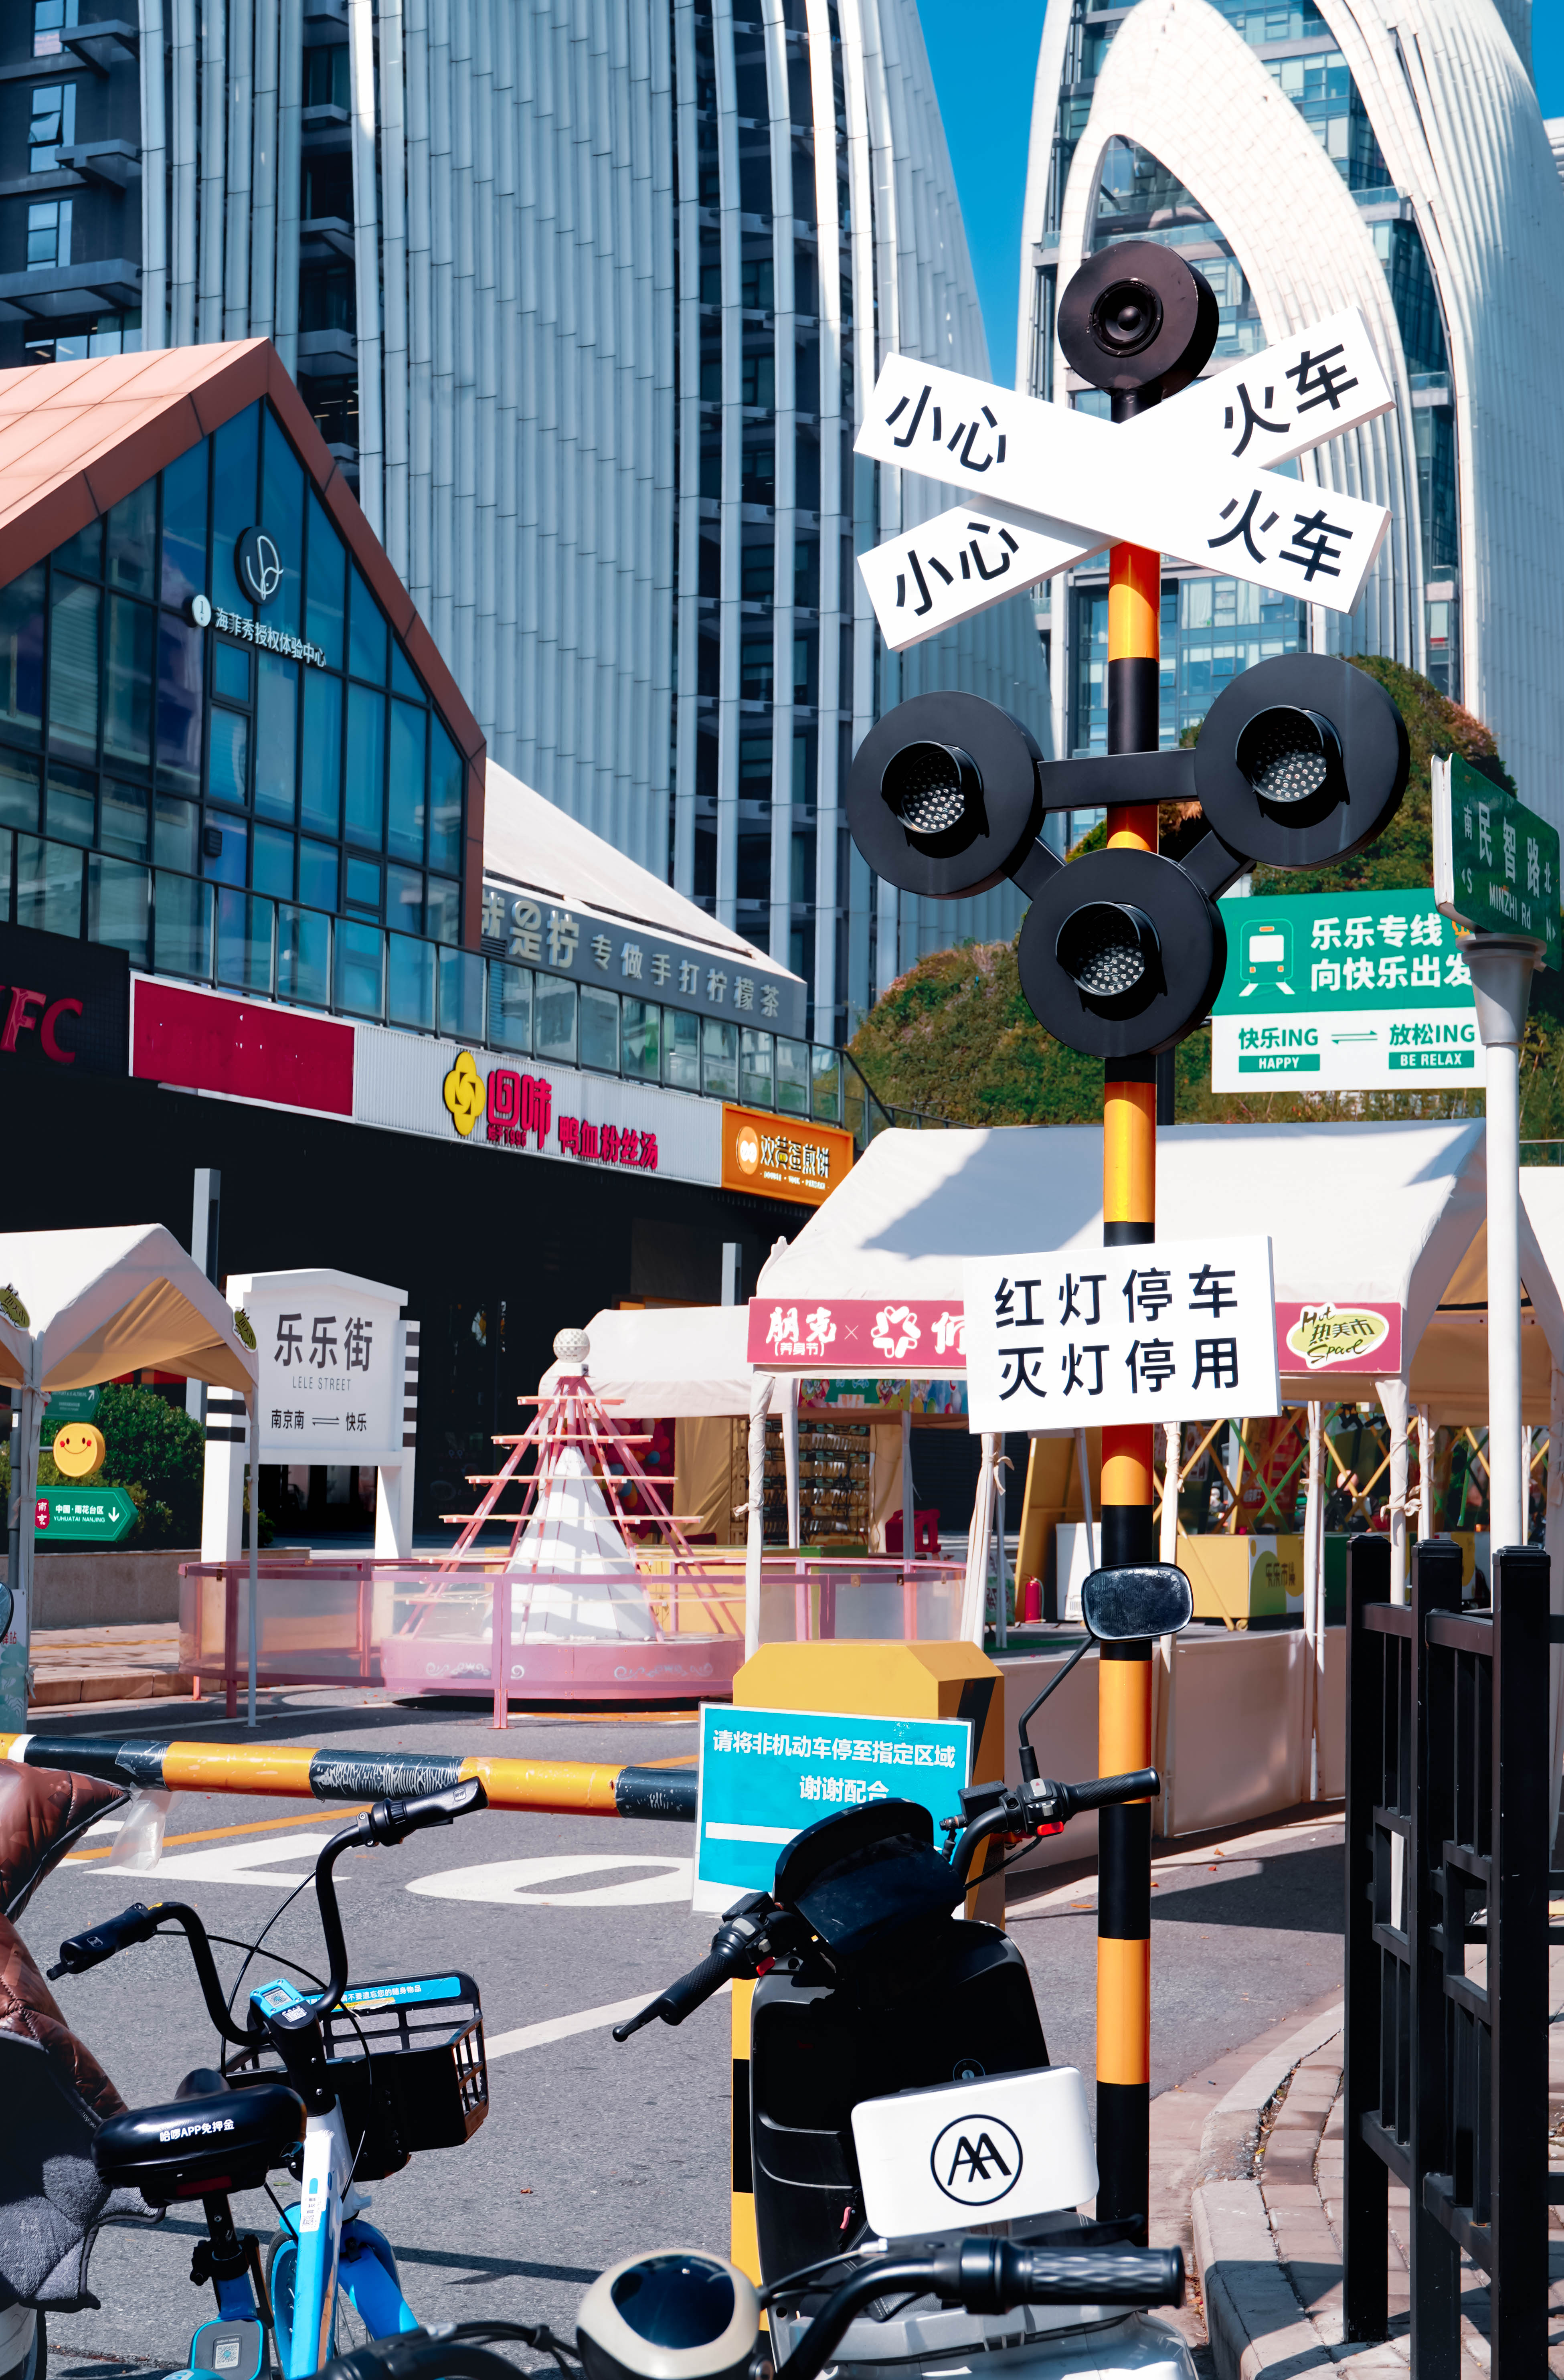
\includegraphics[width=\paperwidth,height=\paperheight]{src/Figures/Arriere_plan/Arriere_plan_Chap_6.jpg}
}

% Rectangle
\AddToShipoutPictureBG*{
  \begin{tikzpicture}[remember picture,overlay]
    \node[fill=white, opacity=0.75, text width=\paperwidth, minimum height=11cm, anchor=north] 
    at ([yshift=-2cm]current page.north) {};
  \end{tikzpicture}
}

% Source
\AddToShipoutPictureFG*{
  \AtPageLowerRight{
    \raisebox{1cm}{
      \hspace{16cm}
      
\begin{tikzpicture}
        \node[fill=white, rounded corners=5pt, inner sep=5pt, align=center] {
          \tiny{Photographie~: \textcolor{blue}{Dylan Moinse (2024)}}
        };
      \end{tikzpicture}
    }
  }
}

    % ___________________________________________
    % Mini-sommaire
    \cleardoublepage
    \setcounter{tocdepth}{2}
    % Redéfinir le titre de la table des matières locale
    \renewcommand{\localcontentsname}{Table des matières du chapitre~6}
\localtableofcontents

% Réinitialiser numérotation section
\setcounter{section}{0}

    % ___________________________________________
    % Graphical abstract
    \newpage
\section*{Points clés du chapitre~6
    \label{chap6:graphical-abstract}
    }
    \markright{Préambule du chapitre}{}

\begin{figure}[h!]\vspace*{4pt}
        \caption*{}
        \label{graphical-abstract-chap6}
        \centerline{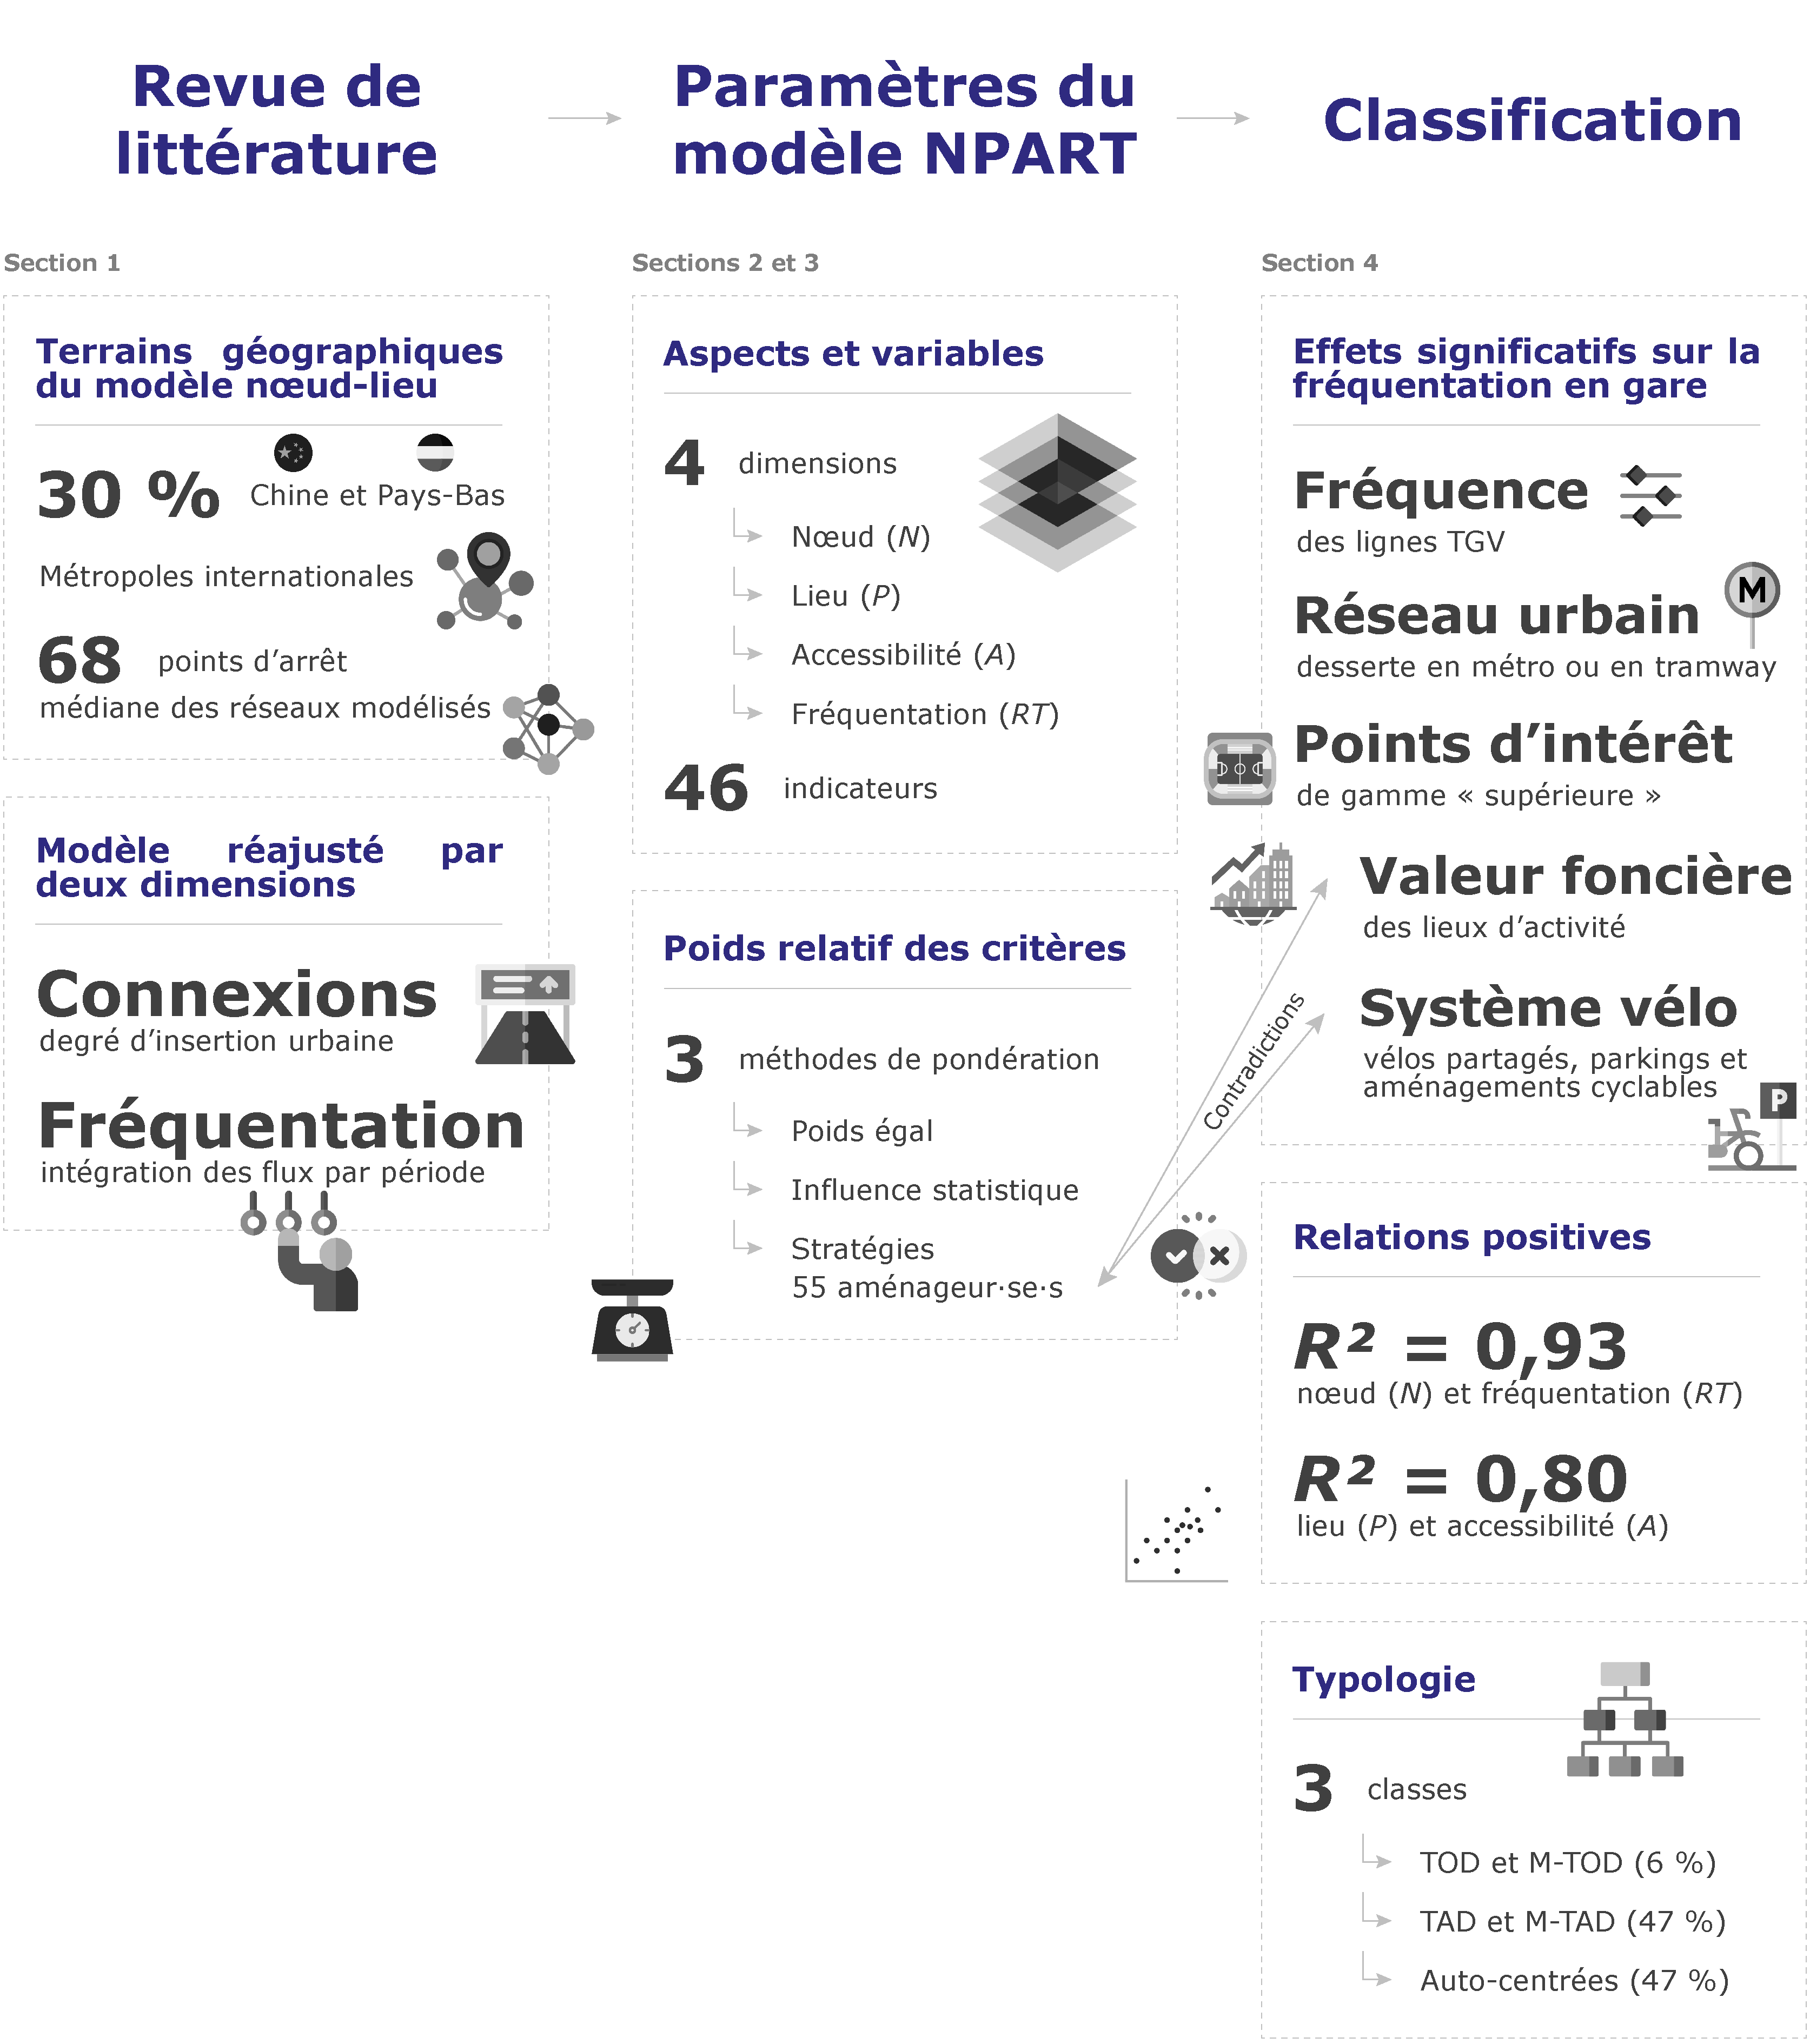
\includegraphics[width=1\columnwidth]{src/Figures/Graphical-abstract/FR_Graphical_abstract_chap6.pdf}}
        \vspace{5pt}
    \end{figure}

    % ___________________________________________
    % Préambule
    \newpage
    \begin{tcolorbox}[colback=white!5!white,
                      colframe=blue!75!blue,
                      title=
                      \bigskip
                      \center{\textbf{Préambule du chapitre~6}}
                      \\
                      \raggedright{\small{Chapitre composé de \pagedifference{chap6:titre}{part3:conclusion} pages, dont \pagedifference{chap6:bibliographie}{part3:conclusion} pages de bibliographie}}
                      \bigskip]
\Large{\textcolor{blue}{\textbf{Résumé~:}}}
    \\
    \small{
Ce chapitre présente une analyse approfondie du potentiel de développement des quartiers de gare dans la région Hauts-de-France, en s'appuyant sur l'application du modèle \Guillemets{nœud-lieu}. Cet outil analytique multicritère évalue le degré d'articulation entre les services de transport en commun et les caractéristiques socio-économiques et urbaines des territoires environnants. Ce modèle permet de cartographier les opportunités de développement en identifiant les relations d'\Guillemets{équilibre} ou de \Guillemets{déséquilibre} entre ces deux dimensions, offrant ainsi une base pour élaborer des stratégies intégrées \acrfull{TOD}.%%Rédigé%%
    \\
Dans un premier temps, nous passons en revue la littérature scientifique pour définir le cadre théorique et méthodologique de cette approche technique (voir la \hyperref[chap6:revue-litterature-m-tod-index]{revue de littérature sur le modèle urbain}, page~\pageref{chap6:revue-litterature-m-tod-index}). Les recherches antérieures se concentrent alors dans des contextes métropolitains, en particulier en Asie et en Europe du Nord. Toutefois, son application dans des territoires peu ou moyennement denses, à une échelle régionale comme celle des Hauts-de-France, reste encore largement sous-exploitée, soulignant la nécessité d'une adaptation méthodologique aux réalités locales. Le modèle revisité, que nous avons nommé \acrfull{NPART} (voir les \hyperref[chap6:selection-indicateurs]{paramètres du modèle} et le \hyperref[chap6:methodologie-m-tod-index]{traitement des données recueillies}, pages~\pageref{chap6:selection-indicateurs} et~\pageref{chap6:methodologie-m-tod-index}), innove de différentes manières~: (i) une application originale dans un terrain géographique peu étudié~; (ii) l'ajout de deux dimensions portant sur la qualité des espaces publics et la fréquentation dynamique des gares~; (iii) une démarche comparative entre les quartiers de gare accessibles à pied et en mobilité individuelle légère~; et (iv) l'intégration de techniques statistiques avancées, tels des outils issus du \textsl{Machine Learning}.%%Rédigé%%
    \\
Les résultats de l’étude apportent plusieurs contributions significatives dans la \hyperref[chap6:resultats-modele]{section exposant les résultats clés} (page~\pageref{chap6:resultats-modele})~: (i) ils démontrent la pertinence du modèle pour diagnostiquer les opportunités de redéveloppement urbain, (ii) ils recentrent les réflexions sur l'importance de redéfinir les échelles géographiques et méthodologiques, (iii) et ils soulignent l'intérêt de développer ce modèle en France, où son application reste très limitée malgré son potentiel pour promouvoir des projets de revitalisation urbaine. L'analyse géostatistique du \acrshort{NPART} a également permis de déterminer les critères urbains les plus influents pour définir et soutenir le concept de \acrshort{TOD} et la déclinaison que nous proposons sous le nom de \acrshort{M-TOD}, couvrant des aspects tels que la qualité du service ferroviaire, l'intensité du développement urbain et l'\gls{accessibilité} par la proximité. Une classification des territoires desservis par le train a été établie, distinguant trois catégories~: les territoires \textsl{orientés} vers le rail, les territoires dont les activités sont \textsl{adjacentes} à l'infrastructure de transport en commun et les territoires \textsl{auto-centrés}. Cette typologie régionale invite à concentrer les efforts sur la deuxième classe qui regroupe la moitié des gares du réseau et qui présente un potentiel \acrshort{TOD}, du point de vue des échelles piétonnière et cyclable.%%Rédigé%%
    }
    \tcblower
\Large{\textcolor{blue}{\textbf{Mots-clés~:}}}
    \\
    \small{
Accessibilité~;
Classification~;
Fréquentation temporelle~;
\Marque{GitHub}~;
Modèle nœud-lieu~;
NPART~;
Point de vue des aménageur·se·s~;
Potentiel \textsl{Transit-Oriented Development}~;
Prédiction~;
\textsl{Python}~;
Radar~;
\textsl{Transit-Adjacent Development}
    }
    \end{tcolorbox}

    % ___________________________________________
    % 6.*.
    \newpage
    \needspace{1\baselineskip} % Réserve de l'espace
    \addcontentsline{toc}{section}{Introduction du chapitre~6}
    \sectionheader{Introduction du chapitre}
\section*{Introduction du chapitre~6
    \label{chap6:introduction}
    }
    %\markright{Introduction du chapitre~6}{}

    % Citation
    \begin{displayquote}
\Guillemets{\textsl{Une partie spécifique de la littérature académique sur le} [\textsl{Transit-Oriented Development}] \textsl{TOD se concentre sur l'identification du potentiel de développement des quartiers de gare, résultant de l'interaction entre les dimensions relatives au transport et à l'usage des sols. Le \Guillemets{modèle nœud-lieu} est le cadre analytique principalement utilisé pour cartographier les opportunités de développement. L'hypothèse sous-jacente à la plupart des études sur le} [modèle nœud-lieu] \textsl{NPM est qu'un inventaire systématique des deux caractéristiques pour un ensemble particulier de stations (le long d'un corridor ou dans une région) fournit des connaissances utiles qui peuvent ensuite éclairer les processus de décision et les politiques de planification urbaine.} [\dots] \textsl{Le modèle permet d'établir des points de référence, de comparer les stations de transport en commun et d'élaborer des stratégies \acrshort{TOD} plus ciblées pour des groupes de nœud}. [\dots] \textsl{Enfin, la classification à 3~000 mètres est la moins similaire aux trois autres} [tailles de quartier de gare]. \textsl{Non seulement il y a une différence significative avec la classification à 800 mètres, mais il existe également une différence marquée avec la classification à 1~200 mètres. Ces résultats suggèrent que les analyses axées sur le TOD prenant appui sur le vélo pourraient révéler des typologies radicalement éloignées de celles traditionnellement induites par la marche, où des périmètres d'étude plus restreints sont généralement exploités.}}\footnote{
    \Guillemets{\textsl{A specific part of the academic literature on TOD focuses on identifying the development potential of transit station areas as an outcome of the interplay between transport and land use dimensions. The ‘node-place model’ is the analytical framework that is predominantly used to map the differentiated development opportunities of station(s) areas(s). The assumption underlying most NPM studies is that a systematic inventory of both characteristics for a particular set of stations (along a corridor or within a region), provides useful knowledge that can subsequently inform evidence-based policy discussions, decision making processes and planning practices.} [\dots] \textsl{The model furthermore allows to benchmark and compare stations and draft more targeted TOD strategies for groups of stations}. [\dots] \textsl{Finally, the 3000 m classification is the least similar to the other three. Not only is there a significant difference with the 800 m classification, there is also a pronounced difference with the 1200 m classification. These results suggest that analyses focused on bicycle-TOD may reveal radically different typology outcomes than the typically walking-induced types of TOD in which typically smaller CAs are used.}} \textcolor{blue}{\autocite[50, 83]{caset_planning_2019}}\index{Caset, Freke|pagebf}.
} [traduction libre]

\textcolor{blue}{Freke} \textcolor{blue}{\textcite[50, 83]{caset_planning_2019}}\index{Caset, Freke|pagebf}. \textsl{Planning for Nodes, Places, and People~: a Strategic Railway Station Development Tool for Flanders}. Thèse de doctorat en Géographie. Université de Gand, Université libre de Bruxelles, 198~p. \url{http://hdl.handle.net/1854/LU-8637955}
    \end{displayquote}

    % Introduction
\lettrine[lines=3, findent=8pt, nindent=0pt]{\lettrinefont L}{e} \acrfull{NPM}, également désigné modèle nœud-lieu, constitue un cadre analytique et opérationnel inscrit dans le courant des recherches sur le \acrfull{TOD}. Il part du présupposé selon lequel les infrastructures de \gls{transport en commun}, lorsqu’elles sont intégrées à leur environnement urbain, peuvent favoriser des formes de développement compactes, accessibles et économiquement dynamiques. Cette perspective invite à considérer les gares comme des catalyseurs de développement local, en fonction de leur connectivité et de l’intensité des activités qui s’organisent autour d’elles. Cette grille d'analyse repose sur deux axes fondamentaux~: l’indice de \textsl{nœud} et l’indice de \textsl{lieu}, dont l’\Guillemets{équilibre} garantit un développement intégré des quartiers de gare \textcolor{blue}{\autocite[202]{bertolini_spatial_1999}}\index{Bertolini, Luca|pagebf}. Cette approche systémique permet d’appréhender la complexité des interactions entre réseaux et territoires, autrement dit l'insertion urbaine des gares à partir d'indicateurs fonctionnels et structurels \textcolor{blue}{\autocite[25]{albertelli_variations_2024}}\index{Albertelli, Marion|pagebf}, sur la base d'un système d'évaluation quantitative \textcolor{blue}{\autocite[47]{chorus_application_2011}}\index{Chorus, Paul|pagebf}\index{Bertolini, Luca|pagebf}.%%Rédigé%%

    % Littérature gaps
Le choix d’un tel outil d’analyse s’explique par sa capacité récente, mais reconnue, à évaluer la relation entre l’intensité de l’offre en transport en commun et celle du système urbain. En cela, nous suivons les recommandations formulées par \textcolor{blue}{\textcite[111]{nigro_land_2019}}\index{Nigro, Antonio|pagebf}\index{Bertolini, Luca|pagebf}\index{Moccia, Francesco Domenico|pagebf} qui soulignent les limites des conceptualisations antérieures du \acrshort{NPM}, notamment l’exclusion du rôle des modes de \gls{rabattement} et, par conséquent, du niveau de connexion des zones d’attraction des gares. Alors que les modèles existants se sont principalement concentrés sur les connexions favorables à la marche combinée, le rôle du \gls{vélo} et de la \gls{micro-mobilité} demeure largement sous-exploré dans le cadre du \acrshort{NPM} \textcolor{blue}{\autocite[2]{zhang_make_2023}}\index{Zhang, Mengyuan|pagebf}\index{Lee, Jinwoo Brian|pagebf}. Par conséquent, la majorité des approches se limite à l’analyse de zones tampons de 800 mètres, rendant ces modèles partiellement obsolètes selon \textcolor{blue}{\textcite[12]{olaru_place_2019}}\index{Olaru, Doina|pagebf}\index{Moncrieff, Simon|pagebf}\index{McCarney, Gary|pagebf}\index{Sun, Yuchao|pagebf}\index{Reed, Tristan|pagebf}\index{Pattison, Cate|pagebf}\index{Smith, Brett|pagebf}\index{Biermann, Sharon|pagebf}. Comme l’illustre le \hyperref[fig-chap6:revue-tailles-aires]{diagramme~\ref{fig-chap6:revue-tailles-aires}} (page~\pageref{fig-chap6:revue-tailles-aires}), les quartiers de gare définis dans les divers modèles \acrshort{NPM} présentent généralement des périmètres spatiaux n’excédant pas un rayon moyen d’un kilomètre. Cette approche se traduit par une prise en compte très limitée, voire quasi inexistante, des modes de déplacement tels que le vélo et la micro-mobilité. La figure met en évidence une prédominance de périmètres micro-géographiques très restreints, perceptible à travers les épaisseurs des plus petits cercles représentés.%%Rédigé%%

    % Figure Littérature tailles quartiers de gare
    \begin{figure}[h!]\vspace*{4pt}
        \caption{Revue des tailles de quartier de gare définies dans le cadre des modèles nœud-lieu.}
        \label{fig-chap6:revue-tailles-aires}
        \centerline{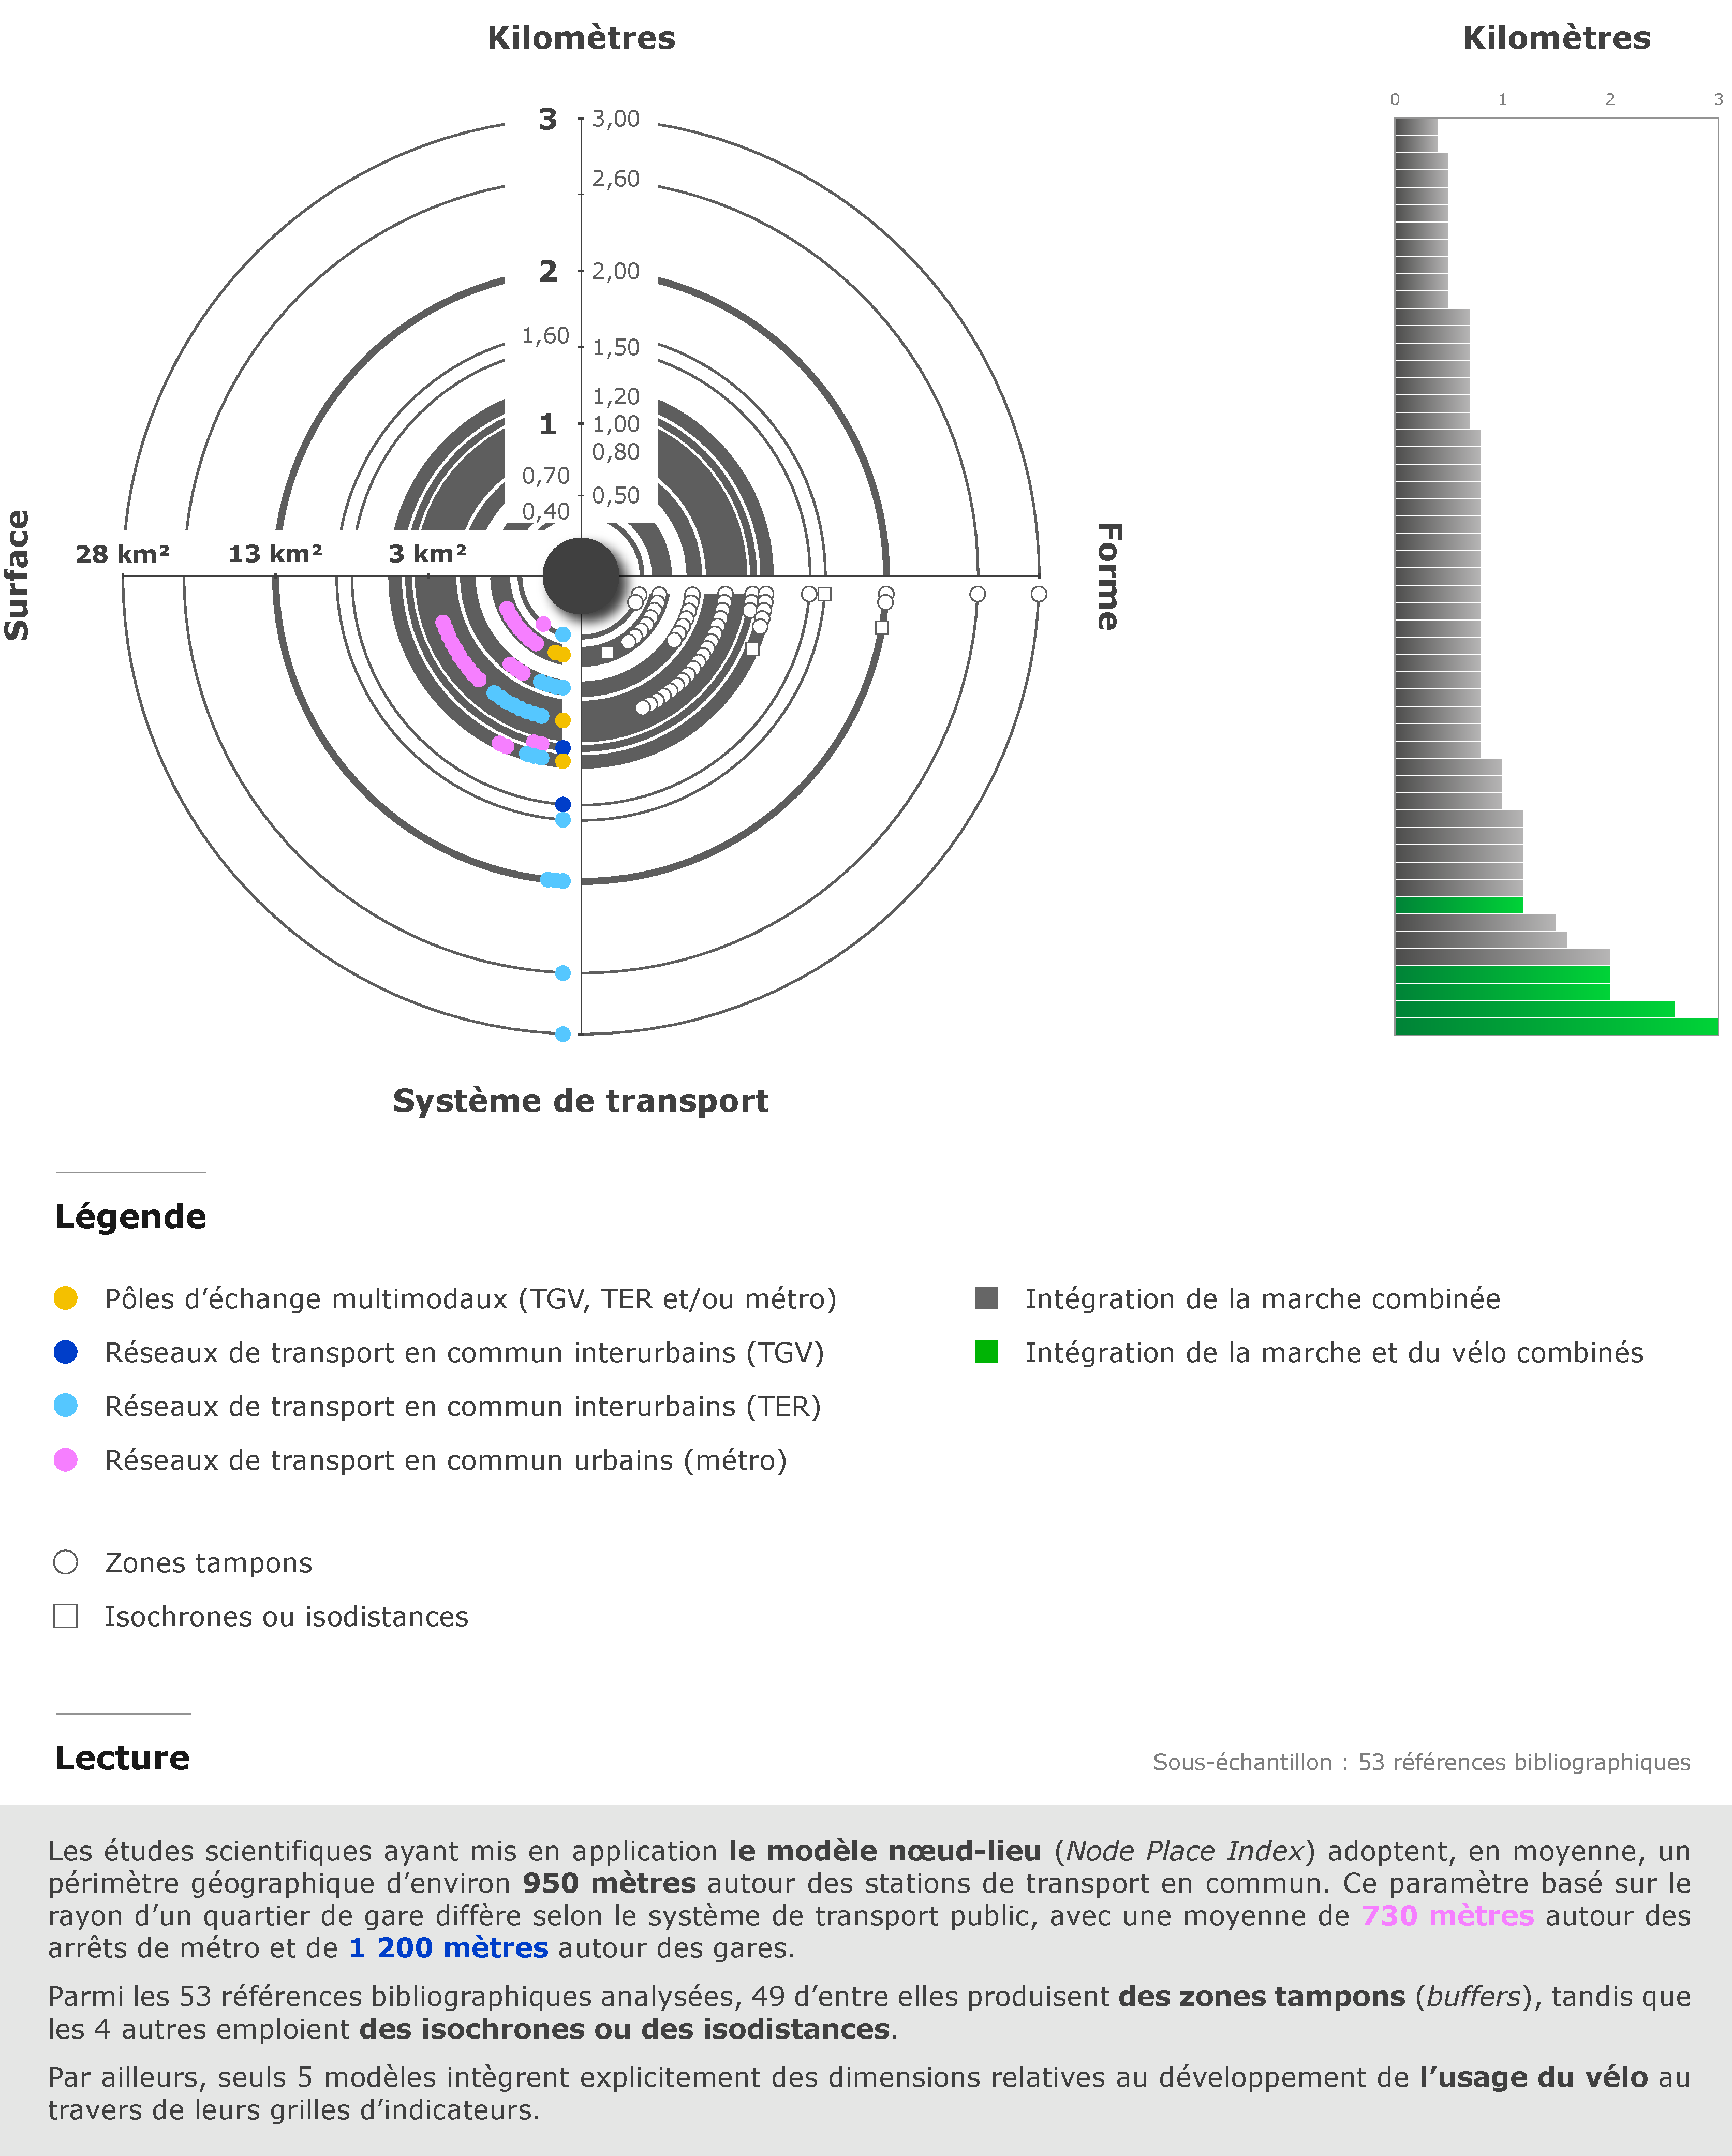
\includegraphics[width=1\columnwidth]{src/Figures/Chap-6/FR_NPART_Distances_quartiers_gare.pdf}}
        \vspace{5pt}
        \begin{flushright}\scriptsize{
        Réalisation~: \textcolor{blue}{Dylan Moinse (2024)}
        \\
        Auteur·rice·s~: projet de recherche \acrshort{NPART}
        }\end{flushright}
    \end{figure}

    % Questionnement général
Ce chapitre se place dans le prolongement des travaux initiés en appliquant le \acrshort{NPM} aux quartiers de gare de la région Hauts-de-France. L’objectif principal est de proposer une lecture avancée du potentiel de développement urbain dans ce terrain d'étude, tout en intégrant nos questionnements de recherche sur l’intégration de la mobilité individuelle légère. Nous nous intéressons ainsi au potentiel de développement des quartiers de gare étudiés. Les principaux sous-objectifs qui guident cette analyse sont les suivantes~:
\begin{customitemize}
    \item \textsl{Contextualisation spatio-temporelle}. Intégrer une perspective intermodale en évaluant la contribution de la mobilité individuelle légère tout en tenant compte des rythmes urbains et en la comparant à l’accessibilité piétonnière~;
    \item \textsl{Calibration du modèle}. Enrichir le modèle existant en y incorporant de nouvelles dimensions pertinentes pour élargir le concept d’aménagement urbain~;
    \item \textsl{Échelle géographique}. Appliquer le modèle révisé à la région Hauts-de-France, marquée par une diversité de formes urbaines~;
    \item \textsl{Statistiques descriptives}. Analyser l’influence des différentes variables sur l’attractivité des gares~;
    \item \textsl{Classification des gares et de leurs environs}. Délimiter et décrire les interactions des nœuds et de leurs abords immédiats pour établir une typologie des stations~;
    \item \textsl{Reproductibilité et automatisation}. Développer un fil conducteur méthodologique à la fois reproductible et automatisé pour la collecte et l’analyse des données géographiques, afin de garantir une appropriation de la modélisation.
\end{customitemize}%%Rédigé%%

    % Annonce du plan 1
Nous ouvrons ce chapitre par une présentation de la revue de littérature sur le \acrshort{NPM}, de manière à faire ressortir les différentes approches adoptées pour évaluer le potentiel de développement des quartiers de gare (\hyperref[chap6:revue-litterature-m-tod-index]{section~1}, page~\pageref{chap6:revue-litterature-m-tod-index}). Cette analyse critique permet principalement d'identifier les contributions et les limites des travaux existants. Dans un premier temps, nous avons situé le modèle dans un cadre conceptuel plus large (\hyperref[chap6:litterature-concept]{sous-section~1.1}, page~\pageref{chap6:litterature-concept}), avant de dresser un panorama des études identifiées afin de retracer l'évolution du modèle au cours des recherches (\hyperref[chap6:litterature-etat-art]{sous-section~1.2}, page~\pageref{chap6:litterature-etat-art}).

    % Annonce du plan 2
À partir des faiblesses identifiées dans la revue de littérature, les paramètres sélectionnés pour notre modélisation sont introduits (\hyperref[chap6:selection-indicateurs]{section~2}, page~\pageref{chap6:selection-indicateurs}). Elle détaille les différentes dimensions et les indicateurs retenus pour la mise en œuvre de notre modèle \acrfull{NPART}. L’analyse s’articule autour des quatre composantes principales du modèle, regroupant un total de 46 indicateurs. Ces dimensions comprennent le nœud (\hyperref[chap6:methodologie-indicateurs-node]{sous-section~2.1}, page~\pageref{chap6:methodologie-indicateurs-node}), le lieu (\hyperref[chap6:methodologie-indicateurs-place]{sous-section~2.2}, page~\pageref{chap6:methodologie-indicateurs-place}), l’accessibilité locale (\hyperref[chap6:methodologie-indicateurs-accessibility]{sous-section~2.3}, page~\pageref{chap6:methodologie-indicateurs-accessibility}) et la fréquentation (\hyperref[chap6:methodologie-indicateurs-frequentation]{sous-section~2.4}, page~\pageref{chap6:methodologie-indicateurs-frequentation}).%%Rédigé%%

    % Annonce du plan 3
La troisième section est dédiée à la collecte et au traitement des données géostatistiques nécessaires à la mise en œuvre du modèle urbain (\hyperref[chap6:methodologie-m-tod-index]{section~3}, page~\pageref{chap6:methodologie-m-tod-index}). Elle expose les différentes techniques utilisées pour l’extraction et la validation des données recueillies (\hyperref[chap6:methodologie-statistiques]{sous-section~3.1}, page~\pageref{chap6:methodologie-statistiques}), puis aborde les méthodes de segmentation et de classification (\hyperref[chap6:methodologie-statistiques-clusterisation-classification]{sous-section~3.2}, page~\pageref{chap6:methodologie-statistiques-clusterisation-classification}), ainsi que les approches de pondération des indicateurs (\hyperref[chap6:methodologie-ponderation-indicateurs]{sous-section~3.3}, page~\pageref{chap6:methodologie-ponderation-indicateurs}).%%Rédigé%%

    % Annonce du plan 4
Avant de conclure ce chapitre, nous engageons une discussion autour des résultats statistiques obtenus à partir d'une situation donnée (\hyperref[chap6:resultats-modele]{section~4}, page~\pageref{chap6:resultats-modele}). En analysant l’influence relative de chaque paramètre du modèle, nous avons pu affiner la définition des modèles \acrshort{TOD} et \acrshort{M-TOD} dans leur essence (\hyperref[chap6:results-influence-indicateurs]{sous-section~4.1}, page~\pageref{chap6:results-influence-indicateurs}). À l’échelle régionale, la modélisation nous a permis de dresser un panorama des gares et de leurs abords, en les classant entre territoires considérés comme \Guillemets{accessibles} ou \Guillemets{dépendants} (\hyperref[chap6:results-caracterisation-gares]{sous-section~4.2}, page~\pageref{chap6:results-caracterisation-gares}). Enfin, ces résultats ont été synthétisés sous forme d’une classification, enrichie par la description des labels attribués à chaque catégorie (\hyperref[chap6:results-classification-gares]{sous-section~4.3}, page~\pageref{chap6:results-classification-gares}).%%Rédigé%%

    % Annonce du plan 5
En clôture, nous assemblons les points clés de ce chapitre construit autour de la conceptualisation et de l’application du modèle \acrshort{NPART}. Ces analyses apportent un éclairage sur le diagnostic du développement actuel et potentiel des gares et de leurs environs, à la fois à l’échelle piétonne et cyclable (\hyperref[chap6:conclusion]{conclusion du chapitre~6}, page~\pageref{chap6:conclusion}).%%Rédigé%%

     % ___________________________________________
    % 6.1.
    \newpage
    \needspace{1\baselineskip} % Réserve de l'espace
    \sectionheader{Revue de littérature du \Guillemets{modèle nœud-lieu}}
\section{Évaluation et classification du potentiel de développement territorial autour des gares par l'intermédiaire du \Guillemets{modèle nœud-lieu}
    \label{chap6:revue-litterature-m-tod-index}
    }

    % Objectifs du NP
Le \acrfull{NPM}, dont le cadre théorique a été exposé par \textcolor{blue}{Luca} \textcolor{blue}{\textcite[343]{bertolini_nodes_1996}}\index{Bertolini, Luca|pagebf} au sein de la Faculté de Géographie de l'Université d'Utrecht, est un outil conçu pour mesurer l'intensité de l'offre en transport en commun associée à un nœud au sein d'un réseau, en lien avec les activités d'un territoire donné. Le \acrshort{NPM} se présente comme un modèle d'analyse multicritère, évaluant les opportunités de redéveloppement tout en intégrant la notion d'\Guillemets{équilibre}, envisagée non seulement à l'échelle d'un quartier de gare, mais aussi dans la perspective globale du réseau de transport en commun, telle qu'illustrée par \textcolor{blue}{Luca} \textcolor{blue}{\textcite[206]{bertolini_spatial_1999}}\index{Bertolini, Luca|pagebf} lors de son application aux agglomérations d'Amsterdam et d'Utrecht. Ce modèle repose sur le principe qu'un indicateur unique est insuffisant pour capturer la complexité territoriale. Cette approche méthodologique requiert donc la considération de multiples dimensions \textcolor{blue}{\autocite[5]{arliani_measuring_2023}}\index{Arliani, Vani|pagebf}\index{Sjafruddin, Ade|pagebf}\index{Santoso, Idwan|pagebf}\index{Winarso, Haryo|pagebf}. Selon \textcolor{blue}{Luca} \textcolor{blue}{\textcite[200]{bertolini_spatial_1999}}\index{Bertolini, Luca|pagebf}, l'ambition du \acrshort{NPM} est de promouvoir une \Guillemets{décentralisation centralisée} (\textsl{centralised decentralisation}), permettant d'étudier les caractéristiques de l'environnement urbain autour des stations de transport en commun afin de favoriser une conception territoriale de type \acrfull{TOD} \textcolor{blue}{\autocite[55]{kamruzzaman_advance_2014}}\index{Kamruzzaman, Md.|pagebf}\index{Baker, Douglas|pagebf}\index{Washington, Simon|pagebf}\index{Turrell, Gavin|pagebf}, et plus particulièrement l'applicabilité de cette stratégie urbaine \textcolor{blue}{\autocites[516-517]{filion_smart_2007}[97]{curtis_delivering_2012}}.%%Rédigé%%

    % Annonce du plan
Dans cette section, nous cherchons à repositionner ce modèle au sein d'une analyse conceptuelle, méthodologique, chronologique et géographique, en questionnant l'intérêt d'une démarche géostatistique de ce type et en synthétisant ses divers apports en relation avec le \acrshort{TOD} ainsi que ses évolutions récentes. Nous allons d'abord nous intéresser au cadre conceptuel et méthodologique qui sous-tend l'objectif du modèle d'examiner les nœuds et leurs environnements (voir la \hyperref[chap6:litterature-concept]{section sur la revue de littérature portant sur cette approche}, page~\pageref{chap6:litterature-concept}). Suivis des différentes contributions existantes, en prenant en compte les contextes géographiques et les interprétations attribuées à ce modèle hautement flexible. L'objectif est ainsi d'identifier, en lien avec notre projet, les lacunes de la littérature actuelle concernant ce modèle ainsi que sa pertinence pour répondre à nos questions de recherche.%%Rédigé%%

    % 6.1.1.
    \needspace{1\baselineskip} % Réserve de l'espace
\subsection{Un cadre méthodologique pour caractériser la coordination entre les services de transport en commun et les dynamiques territoriales
    \label{chap6:litterature-concept}
    }

   % Indices nœuds et lieux
La méthodologie adoptée pour analyser le binôme gare et quartier de gare repose sur la caractérisation du nœud (\textsl{node}) et de son territoire environnant (\textsl{place}), à l'aide de deux indicateurs synthétiques \textcolor{blue}{\autocites[343]{bertolini_nodes_1996}[199]{bertolini_spatial_1999}}\index{Bertolini, Luca|pagebf}. L'articulation de ces deux indicateurs permet d'aborder l'interaction multiscalaire encore peu explorée entre les nœuds des réseaux de transport en commun (\textsl{nodes of networks}) et les lieux urbains (\textsl{places in the city}), d'après \textcolor{blue}{Luca} \textcolor{blue}{\textcite[344]{bertolini_nodes_1996}}\index{Bertolini, Luca|pagebf}. Ce modèle s'avère principalement un \Guillemets{\textsl{outil analytique destiné à identifier le potentiel de développement urbain régional orienté vers les transports en commun}}\footnote{
    \Guillemets{[\dots] \textsl{an analytical tool to help identify the potential for public transport-oriented urban-regional development.}} \textcolor{blue}{\autocite[199-201]{bertolini_spatial_1999}}\index{Bertolini, Luca|pagebf}.
} avec un indice de nœud conçu pour examiner le \Guillemets{potentiel d'interactions humaines physiques} (\textsl{potential for physical human interaction}) et un indice de lieu conçu comme le \Guillemets{degré de réalisation effective de ce potentiel} (\textsl{degree of actual realization of the potential for physical human interaction}), pour reprendre les mots de \textcolor{blue}{Luca} \textcolor{blue}{\textcite[199-201]{bertolini_spatial_1999}}\index{Bertolini, Luca|pagebf}. Fondé sur un modèle de rétroaction, ce cadre d'analyse examine comment l'occupation des sols reflète et bénéficie des avantages du transport public, et \textsl{vice versa} \textcolor{blue}{\autocite[47]{chorus_application_2011}}\index{Chorus, Paul|pagebf}\index{Bertolini, Luca|pagebf}. Le \Guillemets{couple} nœud et lieu repose sur l'idée que l'amélioration de l'offre de transport en commun crée des conditions propices à un développement urbain, qui à son tour intensifie la demande de mobilité, favorisant ainsi le développement du système de mobilité \textcolor{blue}{\autocite[47]{chorus_application_2011}}\index{Chorus, Paul|pagebf}\index{Bertolini, Luca|pagebf}. L'exploration des interrelations entre les divers facteurs peut alors servir d'appui aux politiques publiques en promouvant le \acrshort{TOD} et en proposant une classification qui permettrait d'orienter plus efficacement les investissements dans chaque type de quartier de gare.%%Rédigé%%

    % 6.1.1.1.
    \needspace{1\baselineskip} % Réserve de l'espace
\subsubsection*{Un outil d'analyse de l'accessibilité \textsl{par} et \textsl{autour} des stations de transport en commun
    \label{chap6:litterature-concept-accessibilite}
    }

    % Accessibilité NP
Le modèle \acrshort{NPM} est fondamentalement conçu pour appréhender la notion d'accessibilité, dans le cadre duquel il cherche à examiner les effets conjoints des réseaux de transport (\textsl{network science}) et des caractéristiques de l'environnement urbain (\textsl{spatial science}), une démarche qui fait écho aux perspectives tracées par \textcolor{blue}{\textcite[300]{ducruet_spatial_2014}}\index{Ducruet, César|pagebf}\index{Beauguitte, Laurent|pagebf}. En effet, le modèle mobilise la notion d'accessibilité en partant du postulat qu'un nœud accessible requiert également un lieu accessible, et réciproquement \textcolor{blue}{\autocite[203]{bertolini_spatial_1999}}\index{Bertolini, Luca|pagebf}. Cette approche positionne stratégiquement la station de transport en commun au cœur du réseau auquel elle appartient, en mettant l'accent sur les possibilités de mobilité et les opportunités accessibles qu'elle offre \textcolor{blue}{\autocite[3]{amini_pishro_node_2022}}\index{Amini Pishro, Ahad|pagebf}\index{Yang, Qihong|pagebf}\index{Zhang, Shiquan|pagebf}\index{Amini Pishro, Mojdeh|pagebf}\index{Zhang, Zhengrui|pagebf}\index{Zhao, Yana|pagebf}\index{Postel, Victor|pagebf}\index{Huang, Dengshi|pagebf}\index{Li, WeiYu|pagebf}. Cette vision s'aligne ainsi sur le changement de paradigme auquel participe le \acrshort{TOD} \textcolor{blue}{\autocite[75]{banister_sustainable_2008}}\index{Banister, David|pagebf} et qui valorise un passage d'un aménagement centré sur la mobilité (\textsl{planning for mobility}) à un aménagement centré sur l'accessibilité (\textsl{planning for accessibility}) et dans lequel s'inscrit le modèle \textcolor{blue}{\autocite[496]{caset_measuring_2018}}\index{Caset, Freke|pagebf}\index{Vale, David~S.|pagebf}\index{Viana, Cláudia~M.|pagebf}. Précisons que le modèle se concentre spécifiquement sur la notion d'\Guillemets{accessibilité relative}, telle que définie par \textcolor{blue}{\textcite[27]{dalvi_measurement_1976}}\index{Dalvi,~M.~Q.|pagebf}\index{Martin,~K.~M.|pagebf}, qui se focalise \Guillemets{[\dots] \textsl{non sur l'évolution de l'accessibilité absolue d'un territoire, mais plutôt sur l'évolution de sa position relative par rapport à d'autres territoires, sur une échelle d'accessibilité}}\footnote{
    \Guillemets{\textsl{What is, however, more interesting to note is not the change in the absolute accessibility of different areas when the value of \(\beta\) changes, but the change in their relative position, vis-à-vis each other on the accessibility scale} [\dots]} \textcolor{blue}{\autocite[27]{dalvi_measurement_1976}}\index{Dalvi,~M.~Q.|pagebf}\index{Martin,~K.~M.|pagebf}.
}. Cette perspective comparative de l'accessibilité est également soutenue par \textcolor{blue}{\textcite[521]{caset_measuring_2018}}\index{Caset, Freke|pagebf}\index{Vale, David~S.|pagebf}\index{Viana, Cláudia~M.|pagebf}, qui argumentent que le modèle \acrshort{NPM} met en exergue les possibilités de développement des stations en matière d'urbanisme et de mobilité, en articulant efficacement les réseaux de transport et les dynamiques territoriales. Ce faisant, le \acrshort{NPM} se révèle être un outil analytique puissant pour orienter les politiques publiques et les stratégies d'aménagement urbain, en mettant l'accessibilité au centre de la planification des infrastructures de transport et du développement urbain.%%Rédigé%%

    % Différence TOD Index
L'accessibilité revêt un caractère central dans la conception du \acrshort{NPM}, puisqu'elle vise à éclairer les liens entre la connectivité d'un espace en tant que \textsl{nœud} et ses caractéristiques en tant que \textsl{lieu}. Le choix d'un tel outil appelle à une distinction par rapport à une autre mesure du \acrshort{TOD}, à savoir l'indice \acrshort{TOD} (\textsl{TOD Index})\footnote{
    L'indice \acrshort{TOD} (\textsl{TOD Index}) a été proposé par \textcolor{blue}{\textcite[9]{evans_transit-oriented_2007}}\index{Evans, James|pagebf}\index{Pratt, Richard|pagebf}\index{Stryker, Andrew|pagebf}\index{Kuzmyak,~J.|pagebf} pour mesurer le potentiel \acrshort{TOD} (\textsl{TOD-ness}). Cet indicateur est proposé comme un outil permettant de caractériser le degré auquel un territoire ou un projet répond aux principes du concept d'aménagement. Il a été conçu pour capturer les éléments clés d'un développement dit \Guillemets{réussi} \textcolor{blue}{\autocite[97]{evans_transit-oriented_2007}}\index{Evans, James|pagebf}\index{Pratt, Richard|pagebf}\index{Stryker, Andrew|pagebf}\index{Kuzmyak,~J.|pagebf} pour mesurer le potentiel \acrshort{TOD} (\textsl{TOD-ness}).
}, un indicateur destiné à évaluer la qualité d’un quartier en termes d'accès aux services de transport en commun et de développement urbain. Contrairement au \acrshort{NPM} qui se veut plus analytique, le \textsl{TOD Index} cherche à quantifier dans quelle mesure un territoire adhère aux principes du \acrshort{TOD} \textcolor{blue}{\autocite[3]{pezeshknejad_evaluating_2020}}\index{Pezeshknejad, Parsa|pagebf}\index{Monajem, Saeed|pagebf}\index{Mozafari, Hamid|pagebf}. Selon \textcolor{blue}{\textcite[96]{singh_measuring_2017}}\index{Singh, Yamini Jain|pagebf}\index{Lukman, Azhari|pagebf}\index{Flacke, Johannes|pagebf}\index{Zuidgeest, Mark|pagebf}\index{Maarseveen, Martin van|pagebf}, cet indicateur tend à \textsl{mesurer} le potentiel \acrshort{TOD} \textsl{avant} l'introduction du réseau dans une zone, tandis que le \acrshort{NPM} se concentre sur l'\textsl{évaluation} des quartiers de gare, \textsl{après} le déploiement des systèmes de transport public. En cela, l'indice \acrshort{TOD} s'attache davantage à mesurer le potentiel (\textsl{TOD-ness}) d'une zone à se conformer aux principes du concept d'aménagement, indépendamment de la présence effective d’une station de transport, afin d’établir un indice, plutôt qu’une typologie, finalité du \acrshort{NPM} \textcolor{blue}{\autocite[97, 107]{evans_transit-oriented_2007}}\index{Evans, James|pagebf}\index{Pratt, Richard|pagebf}\index{Stryker, Andrew|pagebf}\index{Kuzmyak,~J.|pagebf}.%%Rédigé%%

    % 6.1.1.2.
    \needspace{1\baselineskip} % Réserve de l'espace
\subsubsection*{Construction d'une typologie des gares et des espaces avoisinants
    \label{chap6:litterature-concept-typologie}
    }

    % Typologie NP
Le cadre analytique du \acrshort{NPM} s'appuie essentiellement sur l'établissement d'une typologie des nœuds, articulée autour du développement d'un indice spatial destiné à évaluer les niveaux de développement urbain et les systèmes de mobilité d'une région. L'élaboration d'une typologie, fondée sur les caractéristiques fonctionnelles des territoires \textcolor{blue}{\autocite[2]{amini_pishro_node_2022}}\index{Amini Pishro, Ahad|pagebf}\index{Yang, Qihong|pagebf}\index{Zhang, Shiquan|pagebf}\index{Amini Pishro, Mojdeh|pagebf}\index{Zhang, Zhengrui|pagebf}\index{Zhao, Yana|pagebf}\index{Postel, Victor|pagebf}\index{Huang, Dengshi|pagebf}\index{Li, WeiYu|pagebf}, suit les principaux objectifs d'une planification orientée vers les transports en commun \textcolor{blue}{\autocite[1]{motieyan_development_2018}}\index{Motieyan, Hamid|pagebf}\index{Mesgari, Mohammad Saadi|pagebf}, soulignant une préoccupation déjà évoquée par \textcolor{blue}{Peter} \textcolor{blue}{\textcite[57]{calthorpe_next_1993}}\index{Calthorpe, Peter|pagebf}. Ce dernier, dans son ouvrage fondateur, distingue les quartiers de gare \Guillemets{urbains} (\textsl{Urban TOD}) des quartiers de gare \Guillemets{de voisinage} (\textsl{Neighborhood TOD}). L'exercice de classification proposé par le modèle se révèle être un outil efficace pour identifier et traiter les obstacles à la mise en application du \acrshort{TOD} \textcolor{blue}{\autocite[55]{kamruzzaman_advance_2014}}\index{Kamruzzaman, Md.|pagebf}\index{Baker, Douglas|pagebf}\index{Washington, Simon|pagebf}\index{Turrell, Gavin|pagebf}. Par ailleurs, la typologie des stations par classe simplifie la compréhension des configurations territoriales, facilitant les comparaisons et la formulation de stratégies transversales qui bénéficient à la fois aux aménageur·se·s, aux gestionnaires de transport et aux acteur·rice·s, tant public·que·s que privé·e·s, impliqué·e·s dans la production urbaine \textcolor{blue}{\autocite[55]{kamruzzaman_advance_2014}}\index{Kamruzzaman, Md.|pagebf}\index{Baker, Douglas|pagebf}\index{Washington, Simon|pagebf}\index{Turrell, Gavin|pagebf}. L'intérêt croissant pour le développement de \Guillemets{typologies normatives du \acrshort{TOD}} (\textsl{normative TOD typologies}) des nœuds traduit une volonté de doter les politiques publiques d'un instrument capable d'éclairer ou d'orienter la planification régionale \textcolor{blue}{\autocite[307]{higgins_forty_2016}}\index{Higgins, Christopher~D.|pagebf}\index{Kanaroglou, Pavlos~S.|pagebf}. Cette typologie vise à évaluer un ensemble de quartiers de gare à l'échelle régionale, en permettant la comparaison entre des stations qui ne présentent pas le même potentiel de développement territorial ni les mêmes besoins en termes de stratégies d'intervention \textcolor{blue}{\autocite[2]{iau_articulation_2017}}\index{IAU@\textsl{IAU}|pagebf}.%%Rédigé%%

    % Comparaison avec d'autres modèles : 4 étapes
Les quartiers \acrshort{TOD}, se manifestant sous diverses formes, nécessitent un outil pratique capable de capturer les caractéristiques spécifiques à chaque cas et permettant des comparaisons entre les différentes entités, afin de formuler des recommandations personnalisées pour atteindre la forme désirée, comme le permet le modèle \acrshort{NPM} \textcolor{blue}{\autocite[270]{li_transit_2019}}\index{Li, Zekun|pagebf}\index{Han, Zixuan|pagebf}\index{Xin, Jing|pagebf}\index{Luo, Xin|pagebf}\index{Su, Shiliang|pagebf}\index{Weng, Min|pagebf}. Celui-ci s'avère être l'approche la plus couramment employée dans les études sur le \acrshort{TOD} pour classer les quartiers de gare au travers de méthodes quantitatives \textcolor{blue}{\autocites[3]{arliani_measuring_2023}[2]{caset_planning_2019}[1]{caset_integrating_2020}[2]{dou_integrating_2021}[113]{ibraeva_transit-oriented_2020}[270]{li_transit_2019}}\index{Arliani, Vani|pagebf}\index{Sjafruddin, Ade|pagebf}\index{Santoso, Idwan|pagebf}\index{Winarso, Haryo|pagebf}\index{Caset, Freke|pagebf}\index{Blainey, Simon|pagebf}\index{Derudder, Ben|pagebf}\index{Boussauw, Kobe|pagebf}\index{Witlox, Frank|pagebf}\index{Dou, Mingxuan|pagebf}\index{Wang, Yandong|pagebf}\index{Dong, Shihai|pagebf}\index{Ibraeva, Anna|pagebf}\index{Almeida Correia, Gonçalo Homem de|pagebf}\index{Silva, Cecília|pagebf}\index{Antunes, António Pais|pagebf}\index{Li, Zekun|pagebf}\index{Han, Zixuan|pagebf}\index{Xin, Jing|pagebf}\index{Luo, Xin|pagebf}\index{Su, Shiliang|pagebf}\index{Weng, Min|pagebf}, les auteur·rice·s \textcolor{blue}{\textcite[578]{banerjee_mobility_2022}}\index{Banerjee, Iman|pagebf}\index{Saha, Apala|pagebf} allant jusqu'à valider ce modèle comme l'un des supports les plus adaptés pour étudier des lieux susceptibles de profiter de stratégies revitalisation urbaine autour de pôles d'échange. Par contraste avec les approches reposant sur des modèles de transport~–~comme le \Guillemets{modèle à quatre étapes}\footnote{
    Le modèle à quatre étapes est une méthode classique dans la modélisation des transports, utilisé pour prévoir la demande de \gls{déplacement} dans une région donnée. Ce modèle structure le processus de planification du transport en quatre étapes séquentielles : (i) évaluation des flux de déplacement générés ou génération, (ii) détermination de leur répartition entre les différentes zones ou distribution, (iii) choix modal et (iv) assignation des déplacements à travers les différents réseaux de transport représentés. Il s'agit d'un modèle urbanisme-transport statique généralement considéré comme technique, complexe et coûteux.
}, focalisé sur la fonction de transport et peu connecté aux usages du sol, tout en consommant des ressources significatives pour sa mise en œuvre~–, l'outil qui nous intéresse se concentre sur les interventions spécifiques au nœud et au lieu qui peuvent influencer la fréquentation du rail \textcolor{blue}{\autocite[2]{caset_integrating_2020}}\index{Caset, Freke|pagebf}\index{Blainey, Simon|pagebf}\index{Derudder, Ben|pagebf}\index{Boussauw, Kobe|pagebf}\index{Witlox, Frank|pagebf}. Le modèle \acrshort{NPM} est apprécié par les chercheur·se·s et par les aménageur·se·s, car il \Guillemets{\textsl{fournit des expressions testables et soutient une analyse et une comparaison plus systématiques}}\footnote{
    \Guillemets{[\dots] \textsl{they provide testable expressions and support more systematic analyses and comparisons.}} \textcolor{blue}{\autocite[41]{lyu_developing_2016}}\index{Lyu, Guowei|pagebf}\index{Bertolini, Luca|pagebf}\index{Pfeffer, Karin|pagebf}.
} \textcolor{blue}{\autocite[41]{lyu_developing_2016}}\index{Lyu, Guowei|pagebf}\index{Bertolini, Luca|pagebf}\index{Pfeffer, Karin|pagebf}, en plus d'orienter les investissements autour des territoires dotés d'un certain potentiel \acrshort{TOD} (\textsl{TOD-ness}), comme expliqué par \textcolor{blue}{\textcite[242]{ibrahim_measuring_2023}}\index{Ibrahim, Sara|pagebf}\index{Ayad, Hany|pagebf}\index{Turki, Eslam|pagebf}\index{Saadallah, Dina|pagebf}. En définitive, la typologie proposée par le modèle permet de dépasser les études de cas isolées, en adoptant une approche à une échelle métropolitaine ou régionale, tout en tenant compte du contexte territorial dans lequel s'intègre le système de transport en commun \textcolor{blue}{\autocite[113]{ibraeva_transit-oriented_2020}}\index{Ibraeva, Anna|pagebf}\index{Almeida Correia, Gonçalo Homem de|pagebf}\index{Silva, Cecília|pagebf}\index{Antunes, António Pais|pagebf}.%%Rédigé%%

    % Figure schéma théorique Node-Place Index
    \begin{figure}[h!]\vspace*{4pt}
        \caption{Diagramme en deux dimensions du modèle nœud-lieu.}
        \label{fig-chap6:schema-theorique-NP}
        \centerline{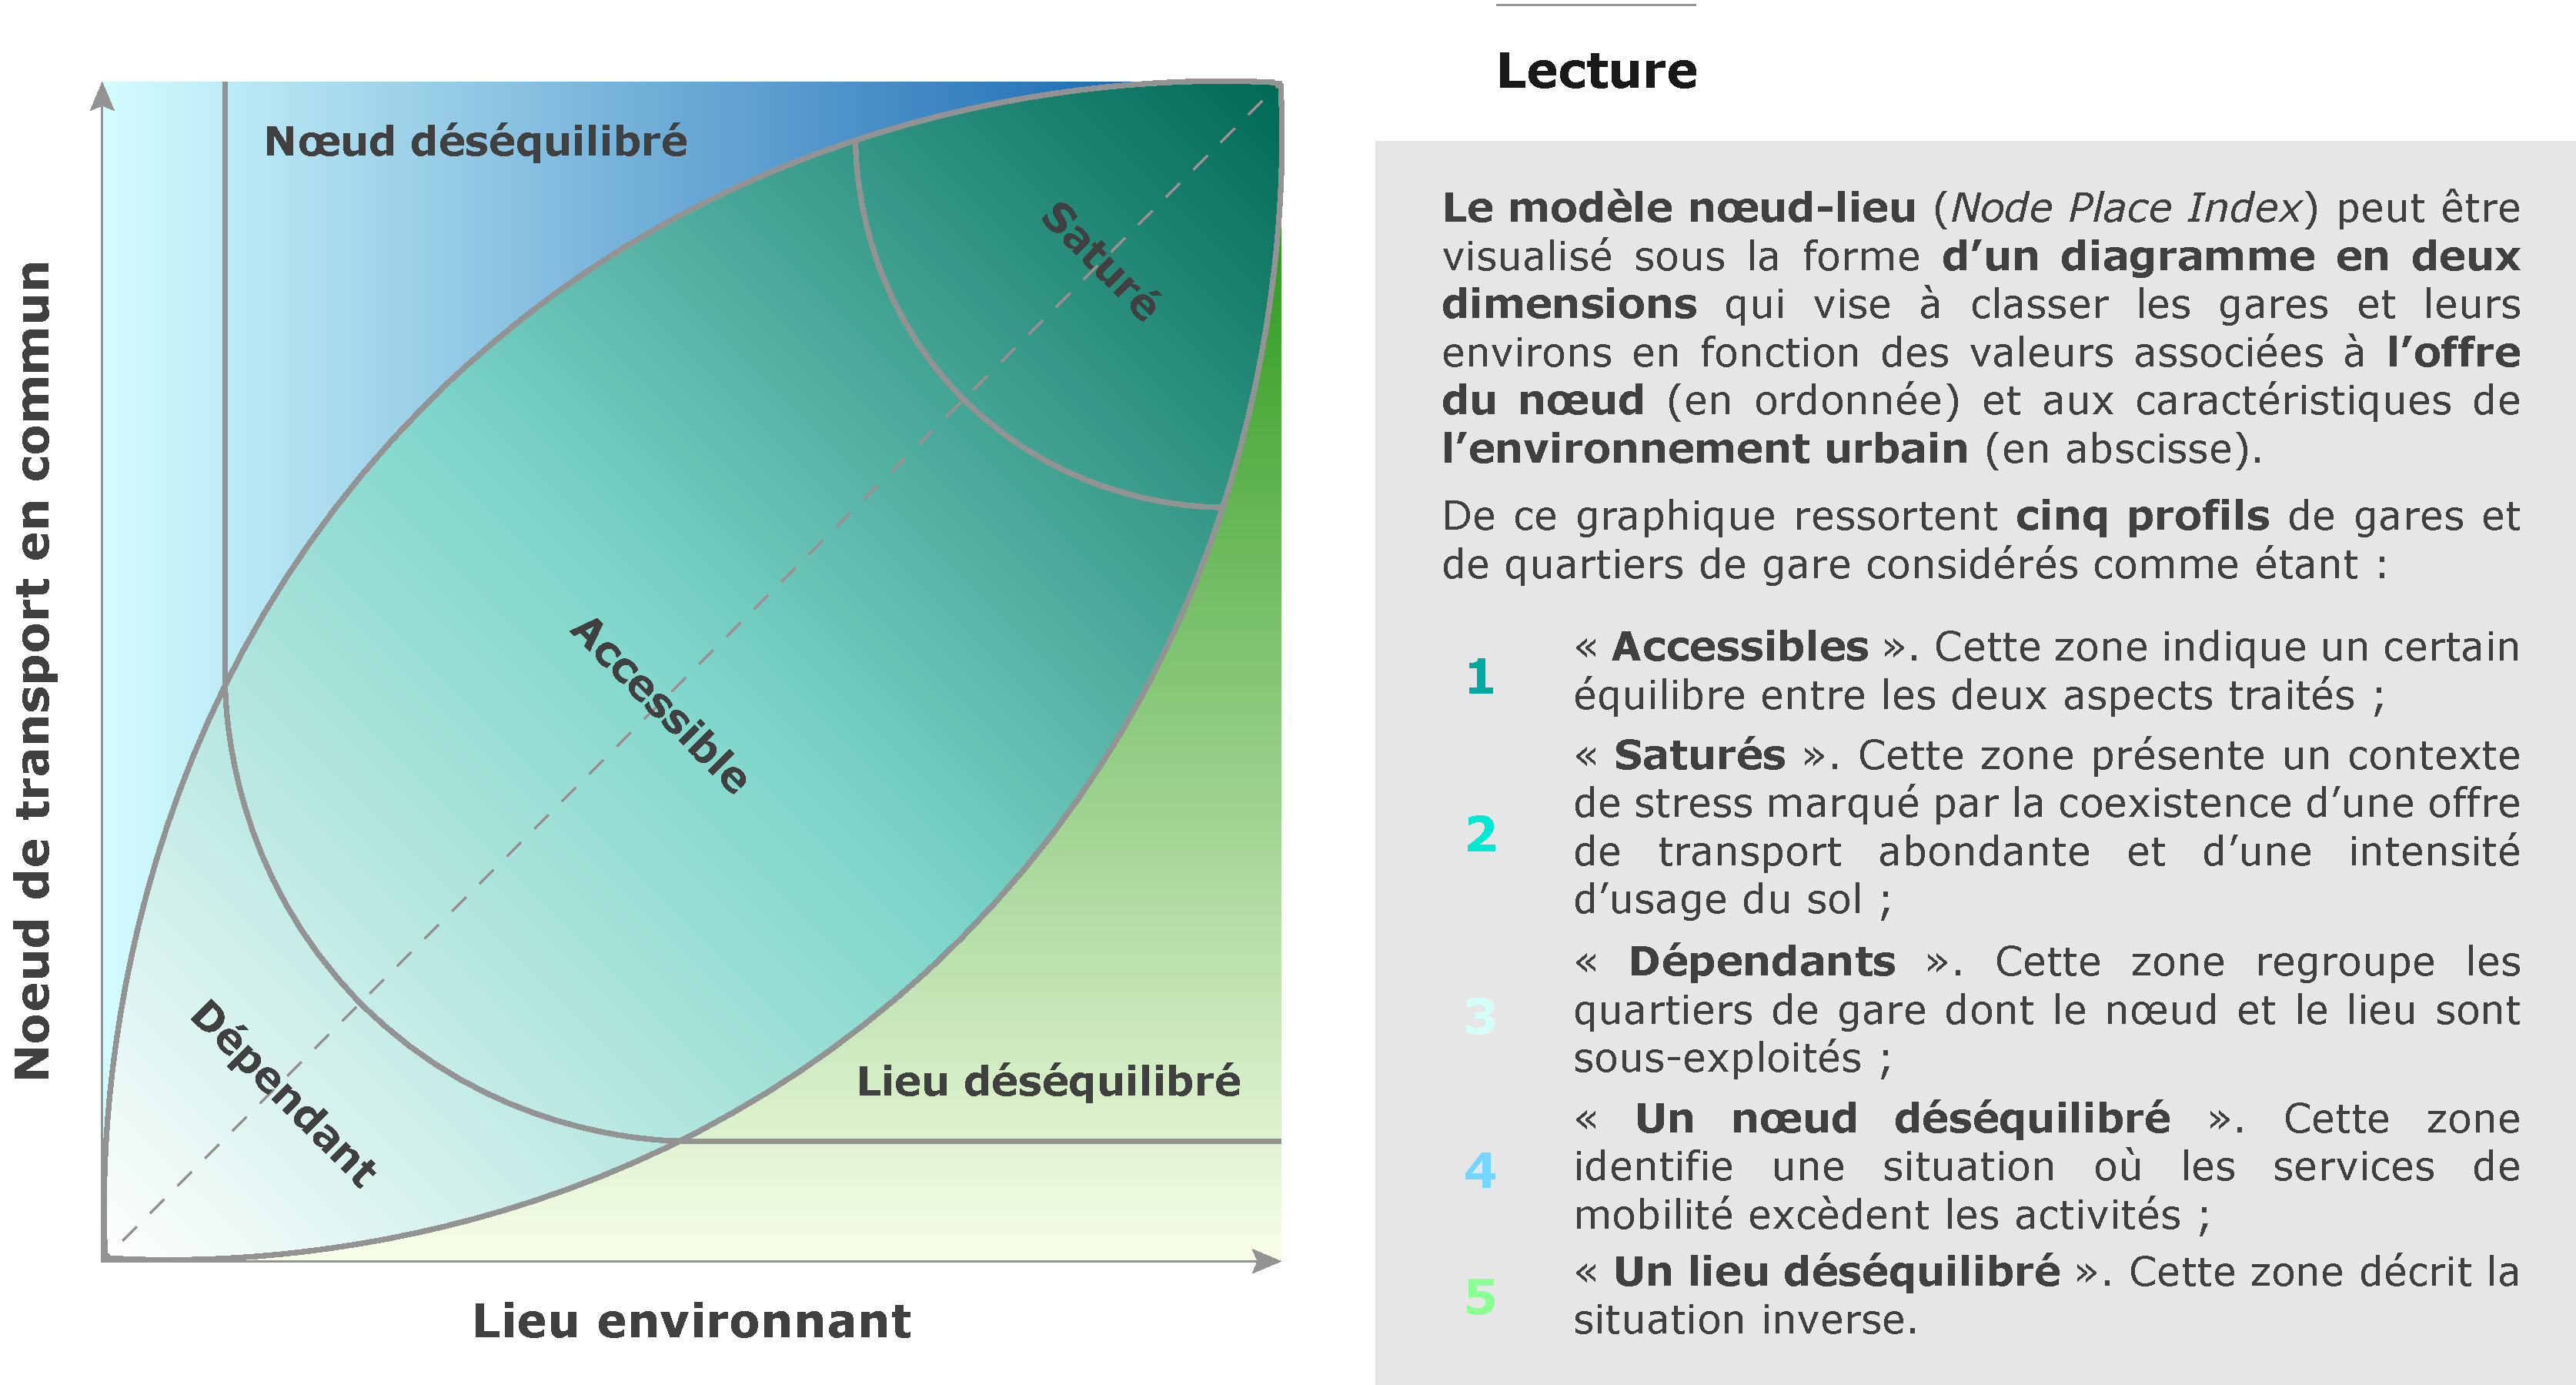
\includegraphics[width=1\columnwidth]{src/Figures/Chap-6/FR_NPART_Diagramme_Bertolini.pdf}}
        \vspace{5pt}
        \begin{flushright}\scriptsize{
        Source~: diagramme réalisé par \textcolor{blue}{Luca} \textcolor{blue}{\textcite[202]{bertolini_spatial_1999}}\index{Bertolini, Luca|pagebf} et réinterprété par \textcolor{blue}{\textcite[243]{yang_tod_2021}}\index{Yang, Liu|pagebf}\index{Song, Xiaoyu|pagebf}
        \\
        Adaptation graphique~: \textcolor{blue}{Dylan Moinse (2024)}
        }\end{flushright}
    \end{figure}

    % Diagramme
Le modèle \acrshort{NPM} propose une lecture diagrammatique et bidimensionnelle pour classifier les nœuds de transport en commun en fonction des caractéristiques observées tant au niveau des arrêts physiques qu'à celui des lieux environnants. Dans ce diagramme initialement développé par \textcolor{blue}{Luca} \textcolor{blue}{\textcite[344]{bertolini_nodes_1996}}\index{Bertolini, Luca|pagebf}, l'intensité de l'usage du sol aux alentours de la station est représentée sur l'axe des abscisses, tandis que l'axe des ordonnées mesure l'accessibilité du nœud. Ce schéma permet de distinguer cinq configurations typologiques distinctes (voir le \hyperref[fig-chap6:schema-theorique-NP]{schéma~\ref{fig-chap6:schema-theorique-NP}}, page~\pageref{fig-chap6:schema-theorique-NP})~:
\begin{customitemize}
    \item La \Guillemets{zone d'équilibre} est identifiée le long de la diagonale centrale du diagramme, signalant une relative équivalence entre les valeurs associées au nœud et celles liées au lieu. La désignation de cette zone est par ailleurs discutée dans la littérature scientifique\footnote{
        En procédant à une classification des gares à Brisbane (Australie), \textcolor{blue}{\textcite[55]{kamruzzaman_advance_2014}}\index{Kamruzzaman, Md.|pagebf}\index{Baker, Douglas|pagebf}\index{Washington, Simon|pagebf}\index{Turrell, Gavin|pagebf} ont confirmé que ces nœuds devraient être classés indépendamment de la notion d'équilibre. Les auteurs illustrent leur propos en présentant deux gares identifiées avec un \Guillemets{potentiel TOD}, dont l'une est équilibrée tandis que l'autre ne l'est pas. De surcroît, selon \textcolor{blue}{\textcite[194]{reusser_classifying_2008}}\index{Reusser, Dominik~E.|pagebf}\index{Loukopoulos, Peter|pagebf}\index{Stauffacher, Michael|pagebf}\index{Scholz, Roland~W.|pagebf}, si un équilibre, tel que défini par \textcolor{blue}{\textcite[202]{bertolini_spatial_1999}}\index{Bertolini, Luca|pagebf}, doit être pris en compte, celui-ci devrait être basé sur la taille des gares, permettant ainsi de mieux contextualiser chacune d'entre elles.
    }, \textcolor{blue}{\textcite[243]{yang_tod_2021}}\index{Yang, Liu|pagebf}\index{Song, Xiaoyu|pagebf} parlant plutôt de \Guillemets{zone accessible}, renvoyant à la définition de l'accessibilité couplant mobilité et environnement urbain~;
    \item La \Guillemets{zone de stress} illustre un contexte au cours duquel l'offre de transport et la diversité des activités humaines sont intenses, générant des interactions maximales~;
    \item La \Guillemets{zone de dépendance} caractérise les quartiers de gare où les valeurs du nœud et du lieu sont cohérentes, mais insuffisamment exploitées~;
    \item La \Guillemets{zone présentant un nœud déséquilibré} est identifiée lorsque les infrastructures et les services de transport excèdent l'usage du sol~;
    \item La \Guillemets{zone présentant un lieu déséquilibré} décrit la situation inverse, où les activités prédominent par rapport à l'offre de transport en commun disponible.
\end{customitemize}%%Rédigé%%

    % Transition
Un modèle tel que le \acrshort{NPM} ne saurait s'accommoder d'une approche universelle, typifiée par l'expression \Guillemets{un modèle générique [pour tous les territoires]} (\textsl{one-size fits all}), surtout lorsqu'il s'agit de mettre en œuvre les principes du \acrshort{TOD}. La nécessité d'adapter les recommandations pour orienter efficacement les politiques publiques exige une analyse approfondie du contexte territorial entourant les stations de transport en commun. Cette approche est appuyée par les travaux de \textcolor{blue}{\textcite[678-679]{zemp_classifying_2011}}\index{Zemp, Stefan|pagebf}\index{Stauffacher, Michael|pagebf}\index{Lang, Daniel~J.|pagebf}\index{Scholz, Roland~W.|pagebf}, dans leur article intitulé \foreignlanguage{english}{\textsl{Classifying railway stations for strategic transport and land use planning: Context matters!}}, où l'importance du contexte géographique est explicitement soulignée dans le processus de classification des gares. À l'inverse, une simplification excessive, qui néglige le contexte spécifique dans lequel chaque station opère, peut conduire à des évaluations erronées, comme le questionnent \textcolor{blue}{\textcite[2]{cao_coordination_2020}}\index{Cao, Zhejing|pagebf}\index{Asakura, Yasuo|pagebf}\index{Tan, Zongbo|pagebf}. La modélisation \acrshort{NPM} met en avant les spécificités locales de chaque site pour un type spécifique de \acrshort{TOD}, plutôt que la question binaire de son adéquation générale, d'après \textcolor{blue}{\textcite[55]{kamruzzaman_advance_2014}}\index{Kamruzzaman, Md.|pagebf}\index{Baker, Douglas|pagebf}\index{Washington, Simon|pagebf}\index{Turrell, Gavin|pagebf}. La capacité de ce modèle à s'ajuster pour refléter plus fidèlement la complexité des environnements urbains dans lesquels les stations de transport sont insérées est dès lors validée par la littérature scientifique, démontrant son applicabilité dans une diversité de contextes urbains.%%Rédigé%%

    % 6.1.2.
    \needspace{1\baselineskip} % Réserve de l'espace
\subsection{État de l'art d'un modèle avancé et graduellement enrichi
    \label{chap6:litterature-etat-art}
    }

    % Intérêt croissant pour le modèle
Depuis 2007, le nombre d'études consacrées à cette approche continue de croître significativement. Cette tendance est mise en évidence dans la revue systématique de la littérature publiée par \textcolor{blue}{\textcite[383]{ibrahim_planning_2022}}\index{Ibrahim, Sara|pagebf}\index{Ayad, Hany|pagebf}\index{Saadallah, Dina|pagebf}. Au cours des vingt dernières années, le modèle a été mis en œuvre dans une variété de contextes géographiques, principalement en Asie de l'Est et du Sud ainsi qu'en Europe du Nord \textcolor{blue}{\autocite[1]{caset_integrating_2020}}\index{Caset, Freke|pagebf}\index{Blainey, Simon|pagebf}\index{Derudder, Ben|pagebf}\index{Boussauw, Kobe|pagebf}\index{Witlox, Frank|pagebf}, et a été adapté à différentes échelles d'application, allant du corridor ferroviaire à la région, et même à l'échelle nationale. Le \acrshort{NPM} a été réalisé aussi bien par des communautés scientifiques que par divers organismes de planification, démontrant ainsi sa flexibilité transcontinentale \textcolor{blue}{\autocite[1]{caset_integrating_2020}}\index{Caset, Freke|pagebf}\index{Blainey, Simon|pagebf}\index{Derudder, Ben|pagebf}\index{Boussauw, Kobe|pagebf}\index{Witlox, Frank|pagebf}.%%Rédigé%%

    % Figure Chronologie NPM
    \begin{figure}[h!]\vspace*{4pt}
        \caption{Évolution chronologique des études sur le modèle nœud-lieu.}
        \label{fig-chap6:litterature-chronologie}
        \centerline{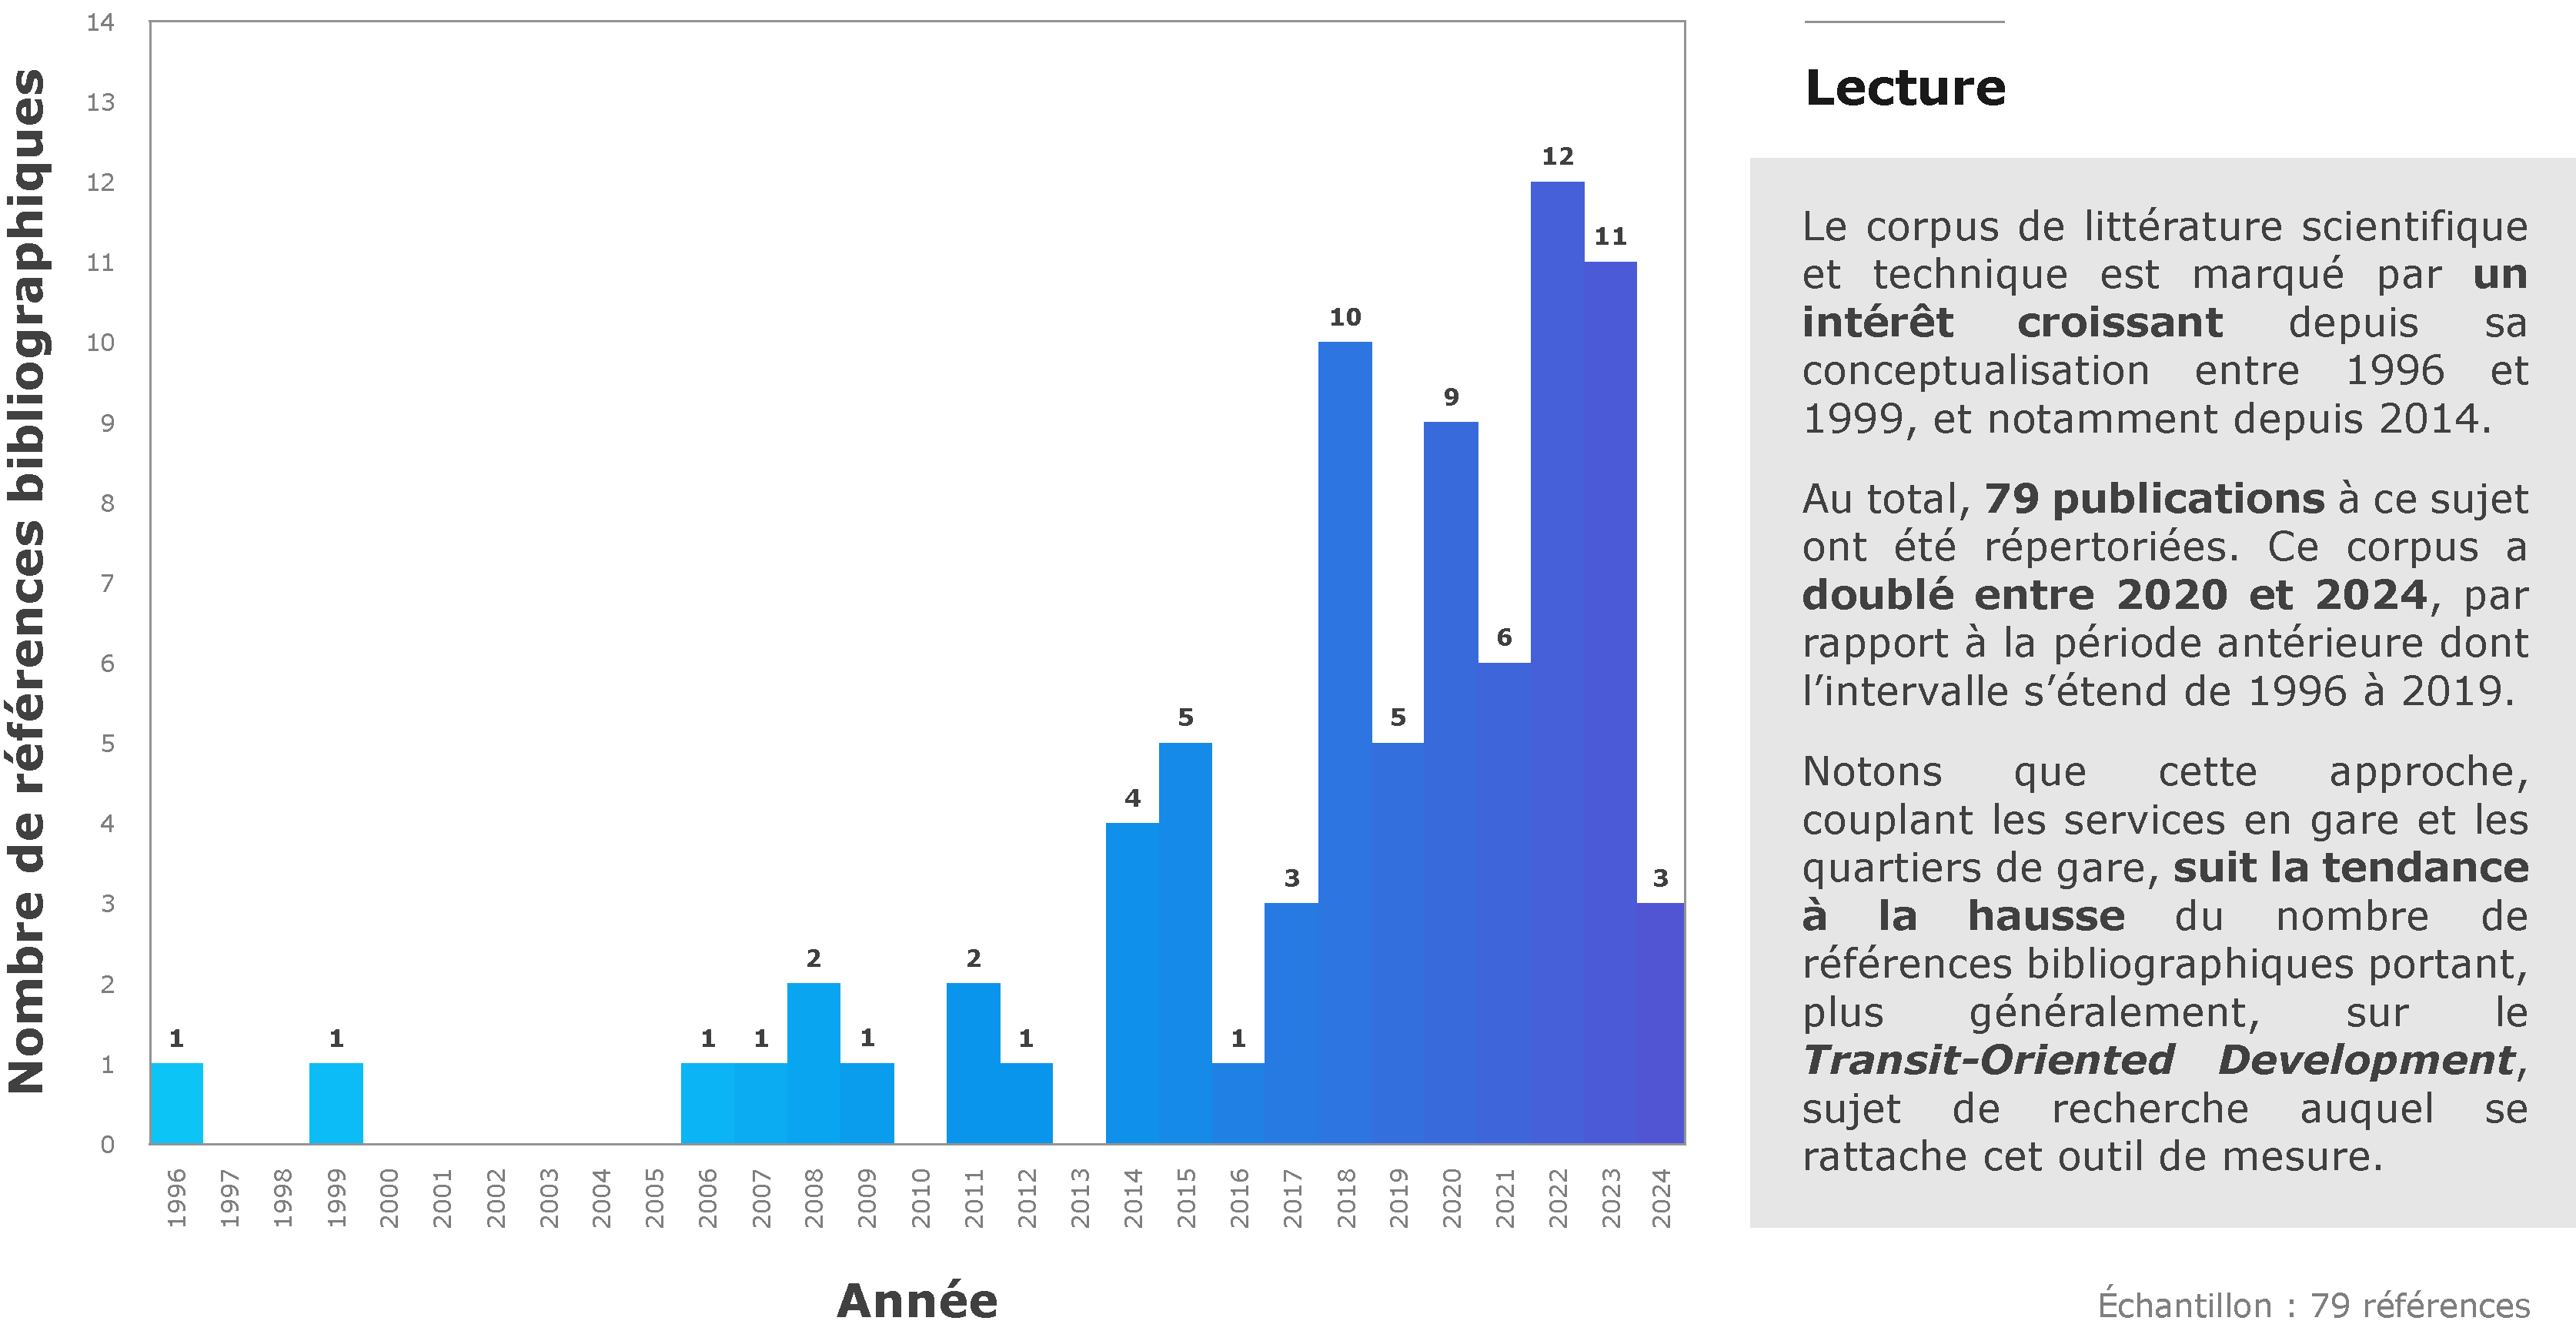
\includegraphics[width=1\columnwidth]{src/Figures/Chap-6/FR_NPART_Chronologie.pdf}}
        \vspace{5pt}
        \begin{flushright}\scriptsize{
        Réalisation~: \textcolor{blue}{Dylan Moinse (2024)}
        \\
        Auteur·rice·s~: projet de recherche \acrshort{NPART}
        }\end{flushright}
    \end{figure}

    % Résultats chronologiques
Dans le cadre de la revue de littérature menée sur le \acrshort{NPM}, nous avons recensé un total de 79 références bibliographiques faisant explicitement usage de cette approche. Ces contributions ont été produites entre 1996, année marquant la conceptualisation du modèle, et le début de l'année 2024, moment où cette recherche bibliographique a été réalisée. Ce corpus comprend ainsi 69 articles, chapitres d’ouvrage collectif et actes de conférences, ainsi que 5 rapports techniques, 3 mémoires de Master et 2 thèses de doctorat. Cette première analyse chronologique confirme l'intérêt croissant pour le \acrshort{NPM} à partir de 2014, avec une dynamique particulièrement marquée entre 2020 et 2024, période durant laquelle le nombre de publications a doublé par rapport à l’intervalle s'étalant de 1996 à 2019 (voir l'\hyperref[fig-chap6:litterature-chronologie]{illustration~\ref{fig-chap6:litterature-chronologie}}, page~\pageref{fig-chap6:litterature-chronologie}). Par ailleurs, cette progression s’inscrit dans la tendance générale de l'augmentation des études portant sur le \acrshort{TOD}.%%Rédigé%%

    % 6.1.2.1.
    \needspace{1\baselineskip} % Réserve de l'espace
\subsubsection*{Une méthode inexploitée dans le contexte français
    \label{chap6:litterature-geographie}
    }

    % Répartition géographique
Les études montrent d’importantes disparités dans l'application du modèle \acrshort{NPM} en fonction des contextes géographiques. Parmi les 63 terrains d’étude identifiés, les contributions sont concentrées en Chine (11 références) et aux Pays-Bas (8 références), de la même manière que la \acrfull{RSL} consacrée à un \acrfull{B-TOD}. À l’inverse, les États-Unis, avec seulement 2 études, sont quasiment absents de ce panorama. Ainsi, l’Asie émerge comme le continent précurseur dans le développement de cet outil quantitatif, comme en témoigne la \hyperref[fig-chap6:repartition-geographique]{carte~\ref{fig-chap6:repartition-geographique}} (page~\pageref{fig-chap6:repartition-geographique}). Par ailleurs, aucune publication scientifique employant ce modèle n'a été répertoriée en France, mis à part une étude conduite par l'Institut d'Aménagement et d'Urbanisme francilien \textcolor{blue}{\autocite[2]{iau_articulation_2017}}\index{IAU@\textsl{IAU}|pagebf}.%%Rédigé%%

    % Carte NP index
    \begin{carte}[h!]\vspace*{4pt}
        \caption{Répartition géographique des études employant le modèle nœud-lieu.}
        \label{fig-chap6:repartition-geographique}
        \centerline{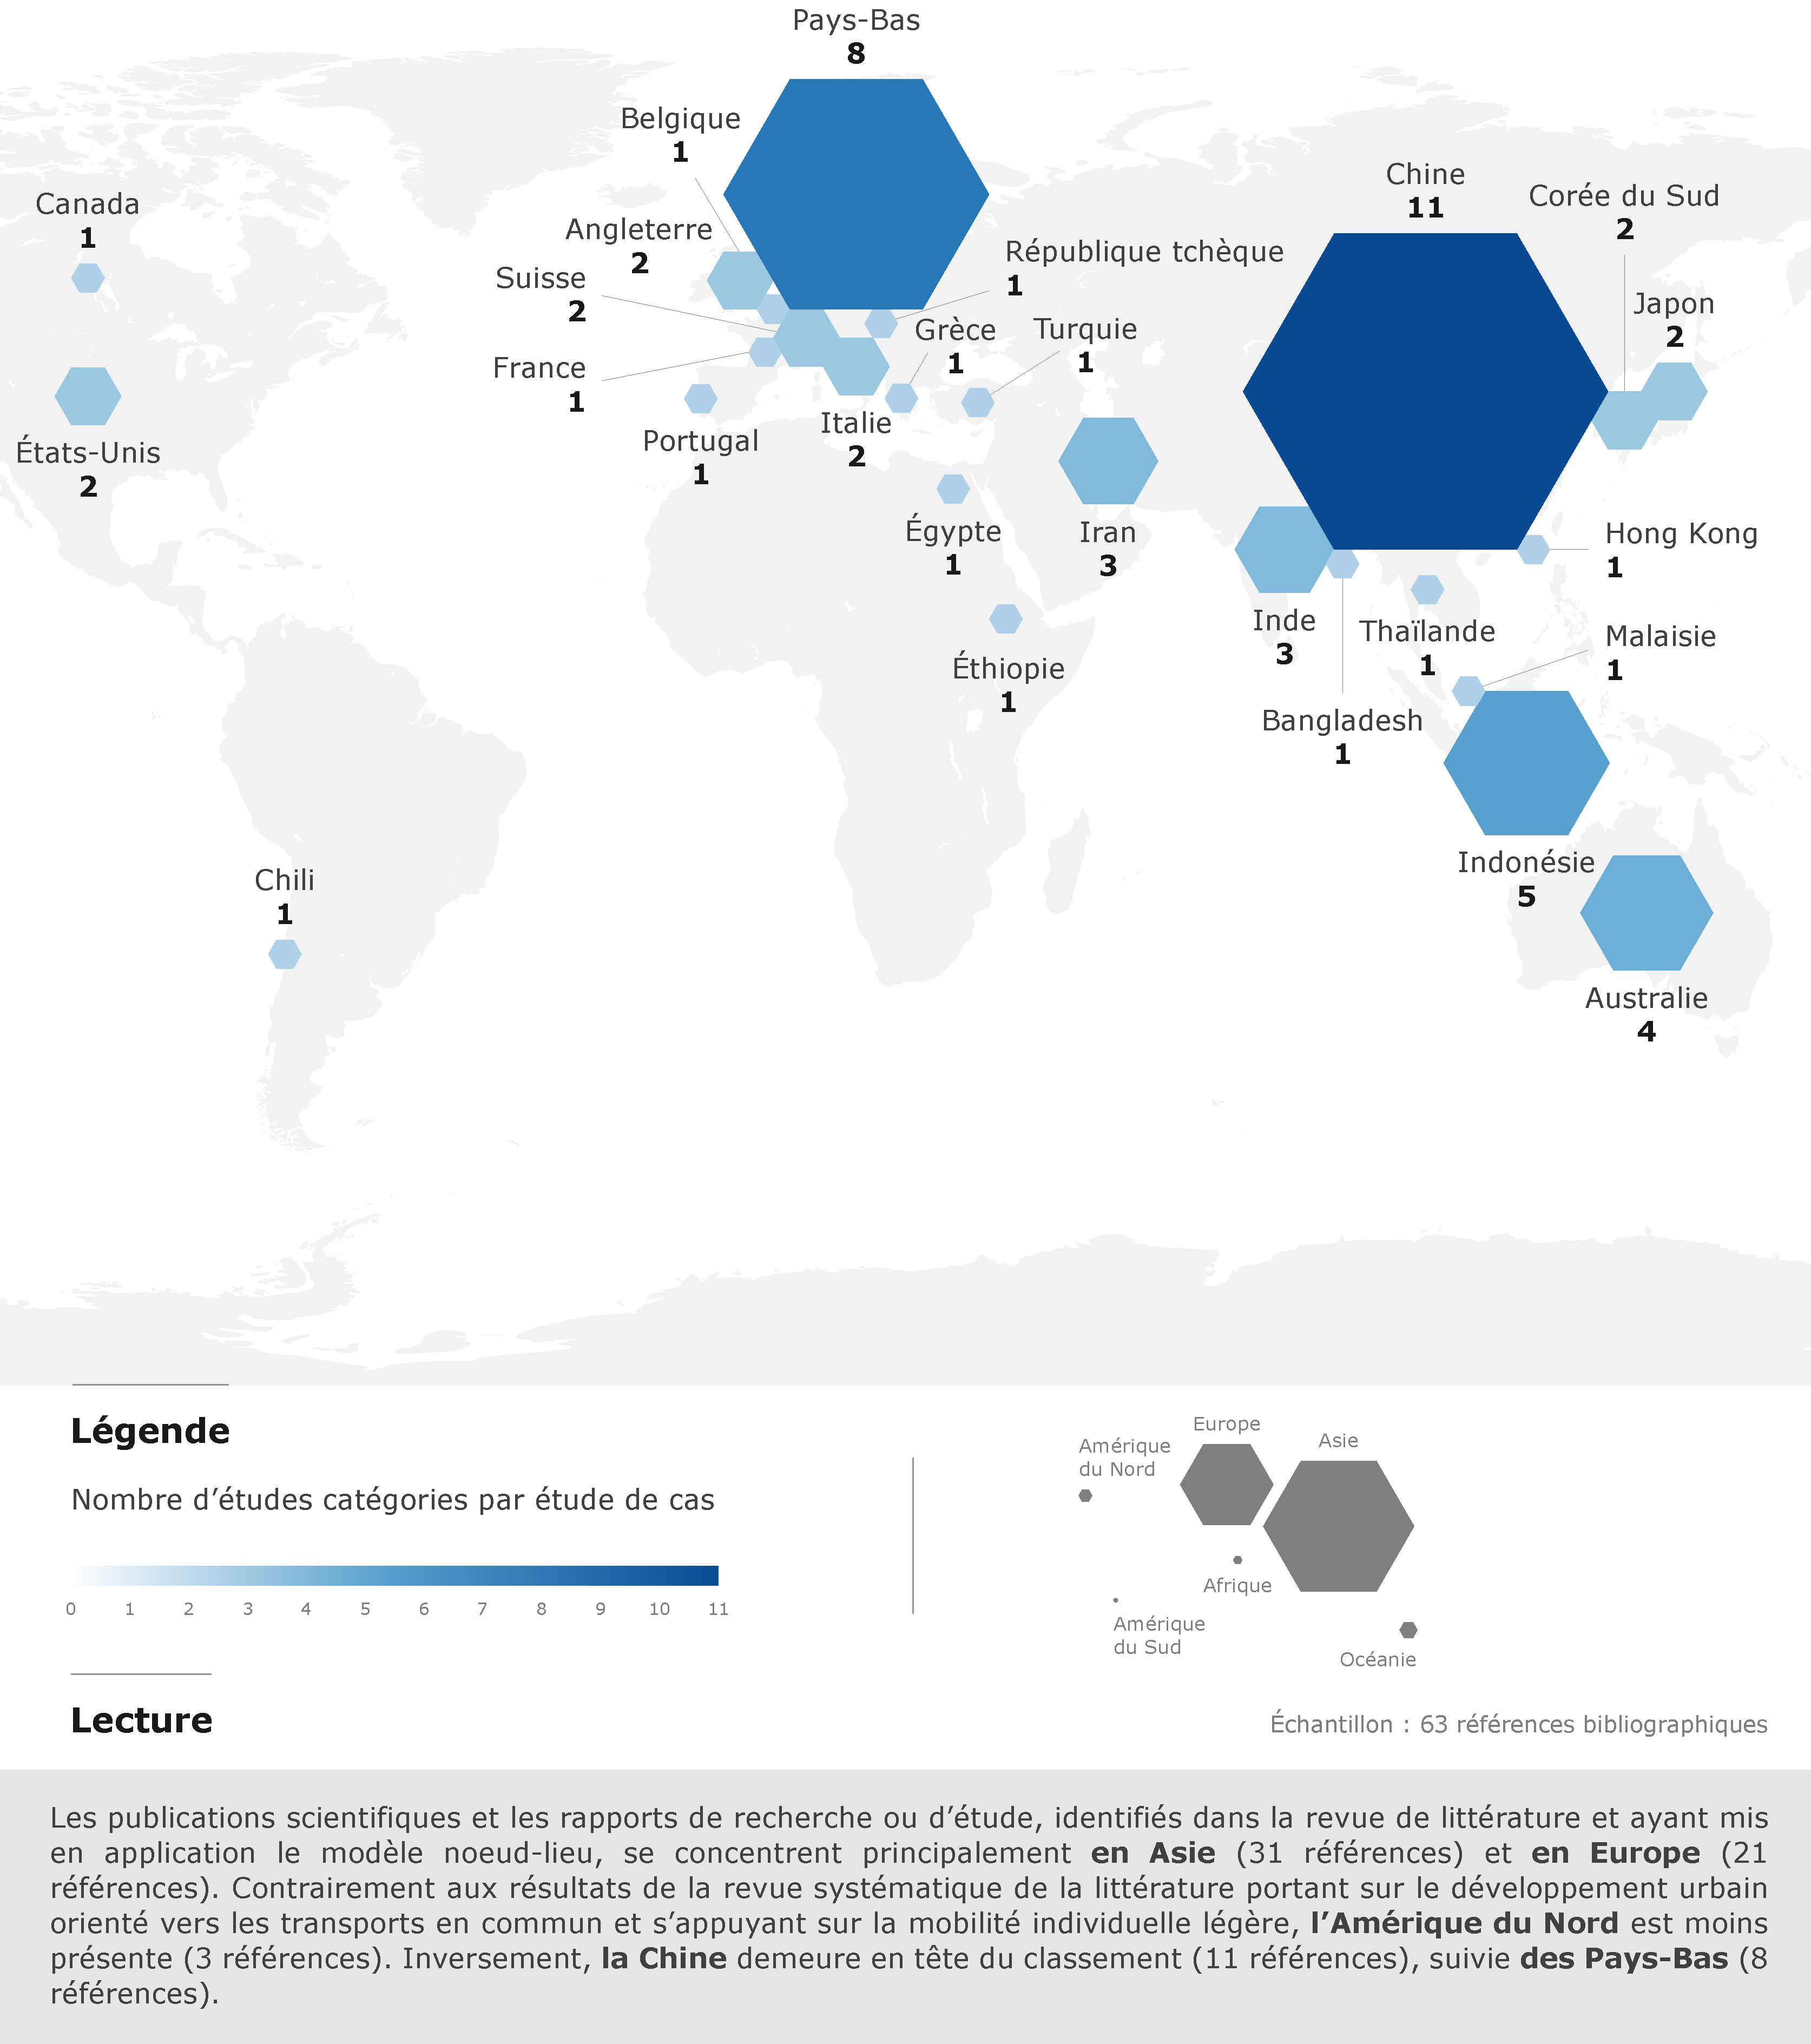
\includegraphics[width=1\columnwidth]{src/Figures/Chap-6/FR_NPART_Repartition_geographique.pdf}}
        \vspace{5pt}
        \begin{flushright}\scriptsize{
        Réalisation~: \textcolor{blue}{Dylan Moinse (2024)}
        \\
        Auteur·rice·s~: projet de recherche \acrshort{NPART}
        }\end{flushright}
    \end{carte}

    % Etudes par pays : Asie
En Asie, nous avons ainsi identifié 31 contributions académiques et rapports d'étude exploitant le modèle \acrshort{NPM}. La Chine se distingue avec 11 études, mettant en avant des métropoles internationales telles que Beijing \textcolor{blue}{\autocites[5]{liao_evaluating_2022}[43]{lyu_developing_2016}}\index{Liao, Cong|pagebf}\index{Scheuer, Bronte|pagebf}\index{Lyu, Guowei|pagebf}\index{Bertolini, Luca|pagebf}\index{Pfeffer, Karin|pagebf}, Chengdu \textcolor{blue}{\autocites[3]{amini_pishro_node_2022}[3]{amini_pishro_integrated_2023}[2]{ma_node-place_2022}}\index{Ma, Jiexi|pagebf}\index{Shen, Zhongwei|pagebf}\index{Xie, Yi|pagebf}\index{Liang, Pengpeng|pagebf}\index{Yu, Bingjie|pagebf}\index{Chen, Li|pagebf}\index{Amini Pishro, Ahad|pagebf}\index{Yang, Qihong|pagebf}\index{Zhang, Shiquan|pagebf}\index{Amini Pishro, Mojdeh|pagebf}\index{Zhang, Zhengrui|pagebf}\index{Zhao, Yana|pagebf}\index{Postel, Victor|pagebf}\index{Huang, Dengshi|pagebf}\index{Li, WeiYu|pagebf}\index{Amini Pishro, Ahad|pagebf}\index{L'Hostis, Alain|pagebf}\index{Chen, Dong|pagebf}\index{Chen, Mojdeh|pagebf}\index{Amini Pishro, Mojdeh|pagebf}\index{Zhang, Zhengrui|pagebf}\index{Li, Jun|pagebf}\index{Zhao, Yuandi|pagebf}\index{Zhang, Lili|pagebf}\index{Shen, Zhongwei|pagebf}\index{Xie, Yi|pagebf}\index{Liang, Pengpeng|pagebf}\index{Yu, Bingjie|pagebf}\index{Chen, Li|pagebf}, Ningbo \textcolor{blue}{\autocite[246]{yang_tod_2021}}\index{Yang, Liu|pagebf}\index{Song, Xiaoyu|pagebf} et Shanghai \textcolor{blue}{\autocites[446]{chen_node-place_2015}[4]{dou_integrating_2021}[273]{li_transit_2019}[8]{su_deciphering_2022}}\index{Su, Shiliang|pagebf}\index{Wang, Zhuolun|pagebf}\index{Li, Bozhao|pagebf}\index{Kang, Mengjun|pagebf}\index{Li, Zekun|pagebf}\index{Han, Zixuan|pagebf}\index{Xin, Jing|pagebf}\index{Luo, Xin|pagebf}\index{Su, Shiliang|pagebf}\index{Weng, Min|pagebf}\index{Chen, Xueming|pagebf}\index{Lin, Lin|pagebf}\index{Wang, Yandong|pagebf}\index{Dong, Shihai|pagebf}\index{Dou, Mingxuan|pagebf}. Deux approches comparatives ont également été conduites, la première le long du delta du Yangtsé, incluant notamment Shanghai, Nanjing, Wuhan et Chongqing \textcolor{blue}{\autocite[629]{wei_classifying_2023}}\index{Wei, Sheng|pagebf}\index{Wang, Lei|pagebf} et la seconde entre Beijing, Hangzhou, Shanghai, Shenzhen et Wuhan \textcolor{blue}{\autocite[11]{su_transit-oriented_2021}}\index{Su, Shiliang|pagebf}\index{Zhang, Hui|pagebf}\index{Wang, Miao|pagebf}\index{Weng, Min|pagebf}\index{Kang, Mengjun|pagebf}. En Indonésie, le modèle a été appliqué dans 5 études, couvrant les métropoles de Jakarta \textcolor{blue}{\autocites[7]{arliani_measuring_2023}[47]{enjeri_characteristics_2020}[27]{taki_re-assessing_2017}}\index{Arliani, Vani|pagebf}\index{Sjafruddin, Ade|pagebf}\index{Santoso, Idwan|pagebf}\index{Winarso, Haryo|pagebf}\index{Taki, Herika|pagebf}\index{Maatouk, Mohamed|pagebf}\index{Qurnfulah, Emad|pagebf}\index{Enjeri, Tomi|pagebf}\index{Widyawati, Sumadio|pagebf}\index{Ash Shidiq, Iqbal|pagebf}, de Depok \textcolor{blue}{\autocite[5]{sulistyaningrum_transit_2018}}\index{Sulistyaningrum, Subekti|pagebf}\index{Sumabrata, Jachrizal|pagebf} et de Wates \textcolor{blue}{\autocite[15]{alfyan_node-place_2022}}\index{Alfyan, Muhammad Yusuf|pagebf}\index{Widyastuti, Dyah Titisari|pagebf}. En Inde, Delhi \textcolor{blue}{\autocite[6]{phani_kumar_identification_2020}}\index{Phani Kumar, Patnala|pagebf}\index{Ravi Sekhar, Chalumuri|pagebf}\index{Parida, Manoranjan|pagebf}, Ahmedabad \textcolor{blue}{\autocite[1~018]{maheshwari_evaluating_2022}}\index{Maheshwari, Richa|pagebf}\index{Grigolon, Anna|pagebf}\index{Brussel, Mark|pagebf} et Noida \textcolor{blue}{\autocite[2]{kapoor_develop_2022}}\index{Kapoor, Sahil Singh|pagebf}\index{Brar, Tejwant Singh|pagebf} ont été les sujets de 3 études, tandis qu'en Iran, Téhéran a été représentée à travers 3 productions scientifiques \textcolor{blue}{\autocites[16]{monajem_evaluation_2015}[5]{motieyan_development_2018}[3]{pezeshknejad_evaluating_2020}}\index{Monajem, Saeed|pagebf}\index{Ekram Nosratian, Farzan|pagebf}\index{Motieyan, Hamid|pagebf}\index{Mesgari, Mohammad Saadi|pagebf}\index{Pezeshknejad, Parsa|pagebf}\index{Monajem, Saeed|pagebf}\index{Mozafari, Hamid|pagebf}. Les autres régions asiatiques se composent de Séoul, en Corée du Sud \textcolor{blue}{\autocites[129]{kim_geographic_2018}[2]{rodriguez_typology_2020}}\index{Rodríguez, Daniel~A.|pagebf}\index{Kang, Chang-Deok|pagebf}\index{Kim, Hyojin|pagebf}\index{Sultana, Selima|pagebf}\index{Weber, Joe|pagebf}, de Tokyo, au Japon \textcolor{blue}{\autocites[3]{cao_coordination_2020}[48]{chorus_application_2011}}\index{Chorus, Paul|pagebf}\index{Bertolini, Luca|pagebf}\index{Cao, Zhejing|pagebf}\index{Asakura, Yasuo|pagebf}\index{Tan, Zongbo|pagebf}, de Bangkok, en Thaïlande \textcolor{blue}{\autocite[120]{supaprasert_transit-oriented_2021}}\index{Supaprasert, Srisamrit|pagebf}\index{Lohatepanont, Manoj|pagebf}\index{Visamitanan, Krisana|pagebf}, de Dacca, au Bangladesh \textcolor{blue}{\autocites[11]{uddin_framework_2023}[6]{uddin_revolutionizing_2023}}\index{Uddin, Md Anwar|pagebf}\index{Hoque, Md Shamsul|pagebf}\index{Tamanna, Tahsin|pagebf}\index{Adiba, Saima|pagebf}\index{Muniruzzaman, Shah Md|pagebf}\index{Parvez, Mohammad Shahriyar|pagebf}\index{Bin Kabir, Sadib|pagebf}, de Kuala Lumpur, en Malaisie \textcolor{blue}{\autocite[249]{khalid_evaluating_2023}}\index{Khalid, Nurul Shakila|pagebf}\index{Samsudin, Noor Aimran|pagebf} et d'Hong~Kong \textcolor{blue}{\autocite[2]{zhou_introducing_2023}}\index{Zhou, Mingzhi|pagebf}\index{Zhou, Jiali|pagebf}\index{Zhou, Jiangping|pagebf}\index{Lei, Shuyu|pagebf}\index{Zhao, Zhan|pagebf}.%%Rédigé%%

    % Etudes par pays : Europe
En Europe, 21 références bibliographiques ont été analysées, révélant une prépondérance des Pays-Bas, avec 8 recherches, incluant thèses de doctorat et mémoires de Master, parmi lesquelles une étude d'envergure nationale \textcolor{blue}{\autocite[273]{debrezion_modelling_2009}}\index{Debrezion, Ghebreegziabiher|pagebf}\index{Pels, Eric|pagebf}\index{Rietveld, Piet|pagebf}. Ces travaux s'attachent principalement à étudier la région métropolitaine d'Arnhem Nimègue \textcolor{blue}{\autocites[309]{huang_measuring_2018}[11]{lukman_development_2014}[132]{singh_measuring_2014}[24]{singh_measuring_2015}[101]{singh_measuring_2017}[268]{singh_planning_2018}}\index{Huang, Runjie|pagebf}\index{Grigolon, Anna|pagebf}\index{Madureira, Ana Mafalda|pagebf}\index{Brussel, Mark|pagebf}\index{Singh, Yamini Jain|pagebf}\index{Fard, Pedram|pagebf}\index{Zuidgeest, Mark|pagebf}\index{Brussel, Mark|pagebf}\index{Maarseveen, Martin van|pagebf}\index{Flacke, Johannes|pagebf}\index{Lukman, Azhari|pagebf}\index{Lukman, Azhari|pagebf}\index{Singh, Yamini Jain|pagebf} et la région métropolitaine de la Randstad \textcolor{blue}{\autocites[203]{bertolini_spatial_1999}[771]{duffhues_breaking_2014}[8]{groenendijk_incorporating_2018}}\index{Bertolini, Luca|pagebf}\index{Groenendijk, Laura|pagebf}\index{Rezaei, Jafar|pagebf}\index{Almeida Correia, Gonçalo Homem de|pagebf}\index{Duffhues, Jan|pagebf}\index{Mayer, Igor~S.|pagebf}\index{Nefs, Merten|pagebf}\index{Vliet, Mirte van der|pagebf}. Outre les Pays-Bas, d'autres pays européens ont également déployé ce modèle interrogeant l'articulation réseau et urbanisme. En Turquie, les études se sont concentrées sur Ankara \textcolor{blue}{\autocite[5]{ozgur-cevher_evaluating_2020}}\index{Ozgür-Cevher, Ozge|pagebf}\index{Altintasi, Oruc|pagebf}\index{Tuydes-Yaman, Hediye|pagebf}, tandis qu'en Belgique, les études ont englobé les régions de Bruxelles et des Flandres \textcolor{blue}{\autocites[34]{caset_planning_2019}[2]{caset_integrating_2020}[500]{caset_measuring_2018}}\index{Caset, Freke|pagebf}\index{Blainey, Simon|pagebf}\index{Derudder, Ben|pagebf}\index{Boussauw, Kobe|pagebf}\index{Witlox, Frank|pagebf}\index{Vale, David~S.|pagebf}\index{Viana, Cláudia~M.|pagebf}. La région francilienne, en France \textcolor{blue}{\autocite[2]{iau_articulation_2017}}\index{IAU@\textsl{IAU}|pagebf}, Lisbonne, au Portugal \textcolor{blue}{\autocites[73]{vale_transit-oriented_2015}[286]{vale_extended_2018}}\index{Vale, David~S.|pagebf}\index{Viana, Cláudia~M.|pagebf}\index{Pereira, Mauro|pagebf}, Londres \textcolor{blue}{\autocite[4]{zhang_network_2019}}\index{Zhang, Yuerong|pagebf}\index{Marshall, Stephen|pagebf}\index{Manley, Ed.~J.|pagebf} et Manchester \textcolor{blue}{\autocite[4]{zheng_classifying_2023}}\index{Zheng, Lingwei|pagebf}\index{Austwick, Martin Zaltz|pagebf}, en Angleterre, Naples \textcolor{blue}{\autocite[291]{papa_tod_2018}}\index{Papa, Enrica|pagebf}\index{Carpentieri, Gerardo|pagebf}\index{Angiello, Gennaro|pagebf} et la région de Campanie \textcolor{blue}{\autocite[114]{nigro_land_2019}}\index{Nigro, Antonio|pagebf}\index{Bertolini, Luca|pagebf}\index{Moccia, Francesco Domenico|pagebf}, en Italie, Ostrava, en République tchèque \textcolor{blue}{\autocite[142]{ivan_evaluation_2012}}\index{Ivan, Igor|pagebf}\index{Boruta, Tomáš|pagebf}\index{Horak, Jiri|pagebf} et Thessalonique, en Grèce \textcolor{blue}{\autocite[8]{papagiannakis_transit-oriented_2021}}\index{Papagiannakis, Apostolos|pagebf}\index{Vitopoulou, Athina|pagebf}\index{Yiannakou, Athena|pagebf} ont aussi fait l'objet d'explorations empiriques. En Suisse, 2 études adoptant une échelle nationale ont été menées \textcolor{blue}{\autocites[194]{reusser_classifying_2008}[672]{zemp_classifying_2011}}\index{Reusser, Dominik~E.|pagebf}\index{Loukopoulos, Peter|pagebf}\index{Stauffacher, Michael|pagebf}\index{Scholz, Roland~W.|pagebf}\index{Zemp, Stefan|pagebf}\index{Stauffacher, Michael|pagebf}\index{Lang, Daniel~J.|pagebf}\index{Scholz, Roland~W.|pagebf}, tandis qu'une enquête de \textcolor{blue}{\textcite[74]{papa_accessibility_2015}}\index{Papa, Enrica|pagebf}\index{Bertolini, Luca|pagebf} met en parallèle les villes d'Amsterdam, Helsinki, Munich, Naples, Rome et de Zurich.%%Rédigé%%

    % Etudes par pays : autres continents
En dehors des continents asiatiques et européens, les recherches ayant recours au modèle \acrshort{NPM} sont plus rares. En Australie, les villes de Brisbane \textcolor{blue}{\autocites[57]{kamruzzaman_advance_2014}[4]{lee_passive_2024}}\index{Lee, Jinwoo Brian|pagebf}\index{Salih, Samal Hama|pagebf}\index{Kamruzzaman, Md.|pagebf}\index{Baker, Douglas|pagebf}\index{Washington, Simon|pagebf}\index{Turrell, Gavin|pagebf}, Perth \textcolor{blue}{\autocite[2]{olaru_place_2019}}\index{Olaru, Doina|pagebf}\index{Moncrieff, Simon|pagebf}\index{McCarney, Gary|pagebf}\index{Sun, Yuchao|pagebf}\index{Reed, Tristan|pagebf}\index{Pattison, Cate|pagebf}\index{Smith, Brett|pagebf}\index{Biermann, Sharon|pagebf} et de Sydney \textcolor{blue}{\autocites[3]{cummings_does_2022}[5]{zhang_make_2023}}\index{Cummings, Christopher|pagebf}\index{Mahmassani, Hani|pagebf}\index{Zhang, Mengyuan|pagebf}\index{Lee, Jinwoo Brian|pagebf} ont été explorées. Aux États-Unis, New York City \textcolor{blue}{\autocite[6]{baghestani_application_2023}}\index{Cummings, Christopher|pagebf}\index{Mahmassani, Hani|pagebf}\index{Baghestani, Amirhossein|pagebf}\index{Najafabadi, Shirin|pagebf}\index{Salem, Azarakhsh|pagebf}\index{Jiang, Ziqi|pagebf}\index{Tayarani, Mohammad|pagebf}\index{Gao, Oliver|pagebf} et au Canada, Montréal \textcolor{blue}{\autocite[80]{robillard_transit-oriented_2024}}\index{Robillard, Arianne|pagebf}\index{Boisjoly, Geneviève|pagebf}\index{Lierop, Dea van|pagebf} ont été étudiées. En Égypte, Alexandrie \textcolor{blue}{\autocite[242]{ibrahim_measuring_2023}}\index{Ibrahim, Sara|pagebf}\index{Ayad, Hany|pagebf}\index{Turki, Eslam|pagebf}\index{Saadallah, Dina|pagebf}, en Éthiopie, Addis-Abeba \textcolor{blue}{\autocite[608]{teklemariam_determining_2020}}\index{Teklemariam, Eden Atsbeha|pagebf}\index{Shen, Zhongwei|pagebf} et au Chili, Santiago \textcolor{blue}{\autocite[87]{vecchio_estaciones_2021}}\index{Vecchio, Giovanni|pagebf} ont été traitées par le modèle.%%Rédigé%%

    % Explications répartition géographique
Ces disparités dans la répartition géographique des études peuvent être interprêtées par la définition de stratégies \acrshort{TOD} déclinées en fonction des contextes spécifiques des systèmes de mobilité et des configurations urbaines existantes. Selon \textcolor{blue}{\textcite[]{bertolini_cities_2015}}\index{Bertolini, Luca|pagebf}\index{Spit, Tejo|pagebf} ainsi qu'\textcolor{blue}{\textcite[]{ivan_evaluation_2012}}\index{Ivan, Igor|pagebf}\index{Boruta, Tomáš|pagebf}\index{Horak, Jiri|pagebf}, en Europe, l'approche se concentre principalement sur le réaménagement des quartiers de gare existants, utilisant le modèle pour évaluer à plus large échelle les opportunités de revitalisation des gares et de leurs environnements immédiats. \textcolor{blue}{\textcite[42]{lyu_developing_2016}}\index{Lyu, Guowei|pagebf}\index{Bertolini, Luca|pagebf}\index{Pfeffer, Karin|pagebf} soulignent qu'en Amérique du Nord et en Australie, l'accent est majoritairement mis sur la recentralisation des zones périurbaines autour des arrêts de transport en commun, tandis qu'en Amérique du Sud, le \acrshort{TOD} est souvent perçu comme un moyen de reconnecter et de recentrer le développement urbain déjà dense autour des nœuds. Au contraire, en Asie, \textcolor{blue}{\textcite[42]{lyu_developing_2016}}\index{Lyu, Guowei|pagebf}\index{Bertolini, Luca|pagebf}\index{Pfeffer, Karin|pagebf} considèrent que l'objectif principal du concept d'aménagement est de canaliser la croissance des mégacités le long des corridors de \textsl{mass transit}, afin de maîtriser l'expansion urbaine.%%Rédigé%%

    % 6.1.2.2.
    \needspace{1\baselineskip} % Réserve de l'espace
\subsubsection*{Une évaluation à une échelle géographique limitée
    \label{chap6:litterature-taille-urbaine}
    }

    % Tailles urbaines
Comme le montrent les différentes énumérations d'études réparties par continents et par pays, très peu d'études s'intéressent à la mise en application du modèle \acrshort{NPM} dans des territoires qui ne font pas partie d'une métropole régionale ou internationale. Cette observation corrobore celle de \textcolor{blue}{\textcite[111]{nigro_land_2019}}\index{Nigro, Antonio|pagebf}\index{Bertolini, Luca|pagebf}\index{Moccia, Francesco Domenico|pagebf}, qui souligne la rareté des recherches portant sur la coordination entre le transport public et l'occupation des sols dans des territoires peu ou moyennement denses, en déclin économique ou intégrant des réseaux de \acrfull{TGV}, en raison d'une couverture très étendue qui pose des contraintes.%%Rédigé%%

    % Figure Tailles des réseaux de TC
    \begin{figure}[h!]\vspace*{4pt}
        \caption{Taille des réseaux de transport en commun, en nombre de stations, intégrée dans le modèle nœud-lieu.}
        \label{fig-chap6:taille-reseaux-TC}
        \centerline{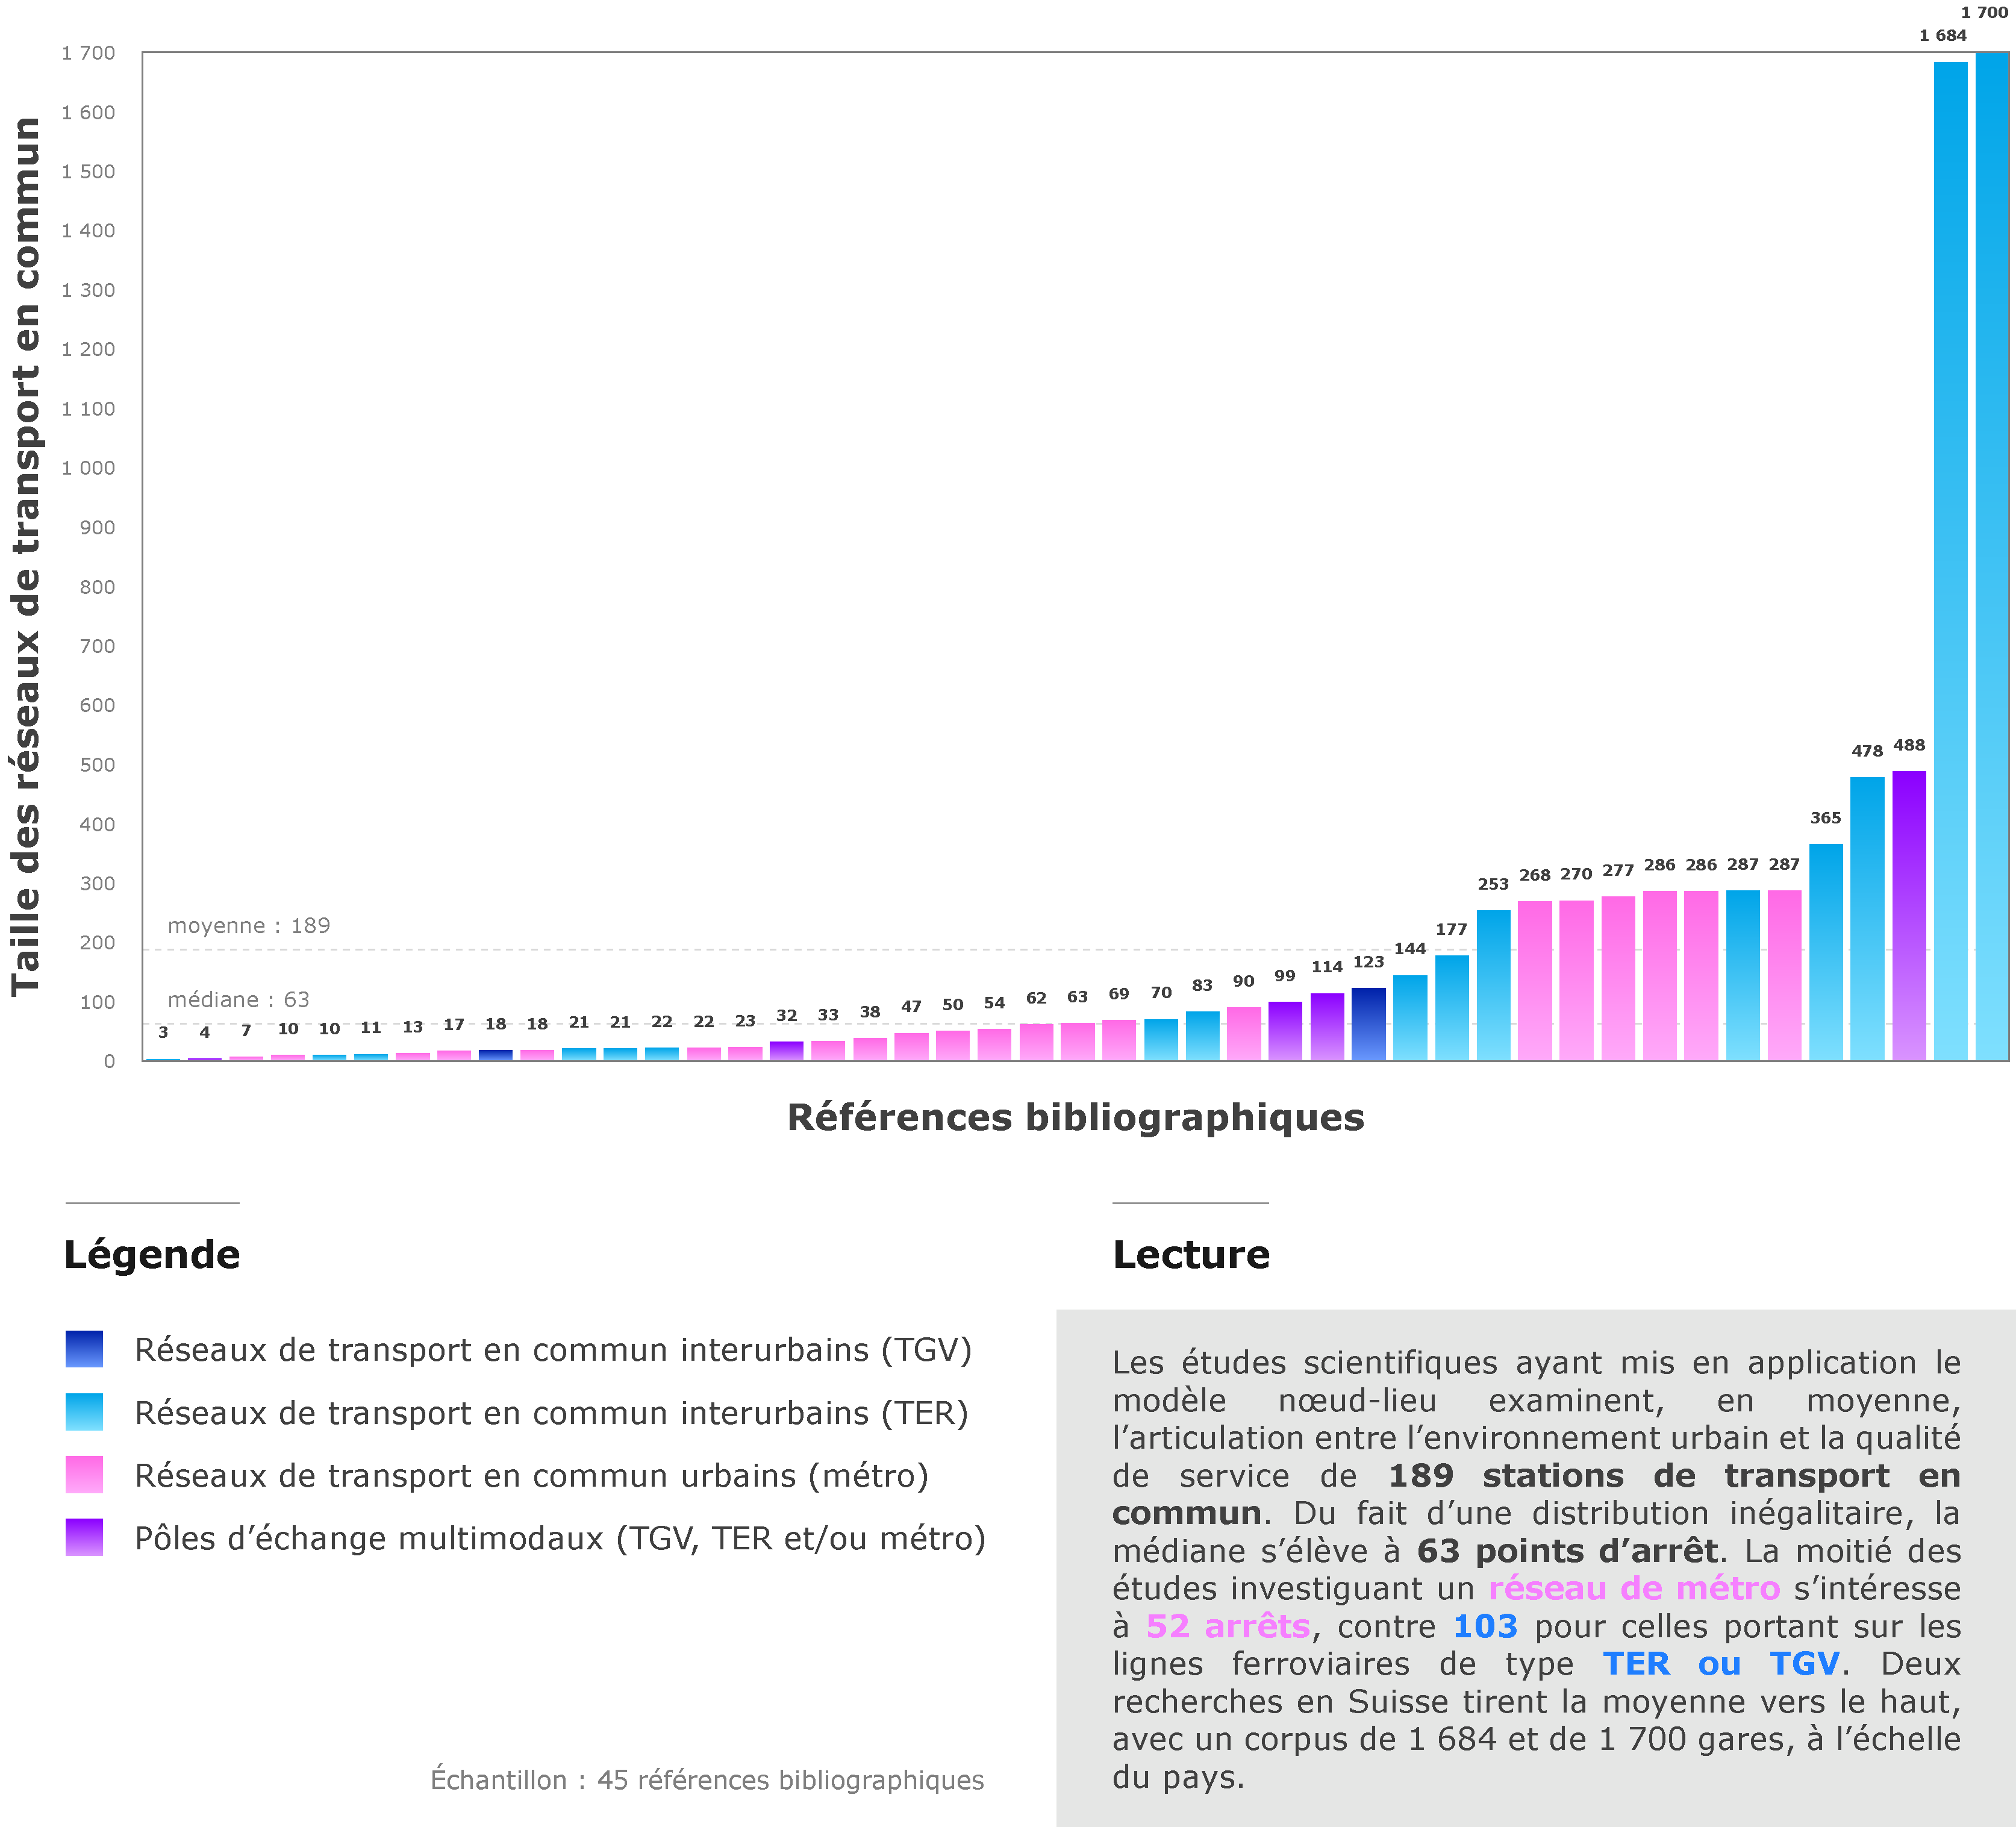
\includegraphics[width=1\columnwidth]{src/Figures/Chap-6/FR_NPART_Taille_reseaux_TC.pdf}}
        \vspace{5pt}
        \begin{flushright}\scriptsize{
        Réalisation~: \textcolor{blue}{Dylan Moinse (2024)}
        \\
        Auteur·rice·s~: projet de recherche \acrshort{NPART}
        }\end{flushright}
    \end{figure}

    % Tailles des réseaux de TC
Une autre démonstration de la flexibilité du modèle en question se manifeste par la diversité de la taille des réseaux de transport en commun examinés, dont les valeurs vont de 3 à 1~700 stations dans un périmètre d'action déterminé. Comme l'illustre le \hyperref[fig-chap6:taille-reseaux-TC]{diagramme~\ref{fig-chap6:taille-reseaux-TC}} (page~\pageref{fig-chap6:taille-reseaux-TC}), cette approche quantitative couvre généralement des systèmes de \acrfull{TER} ou de métro, avec une moyenne de 189 et une médiane de 63 nœuds. En effet, la moitié des études utilisant le \acrshort{NPM} pour l'examen des métros porte sur moins de 52 arrêts, tandis que celles consacrées aux réseaux \acrshort{TER} ou \acrshort{TGV} en couvrent 103. Notons que deux études suisses à l'échelle nationale ont su adapter le modèle à un réseau comprenant approximativement 1~700 gares \textcolor{blue}{\autocites[194]{reusser_classifying_2008}[672]{zemp_classifying_2011}}\index{Zemp, Stefan|pagebf}\index{Stauffacher, Michael|pagebf}\index{Lang, Daniel~J.|pagebf}\index{Scholz, Roland~W.|pagebf}\index{Reusser, Dominik~E.|pagebf}\index{Loukopoulos, Peter|pagebf}\index{Stauffacher, Michael|pagebf}\index{Scholz, Roland~W.|pagebf}.%%Rédigé%%

    % Transition
L'adaptabilité du modèle aux divers contextes géographiques et aux différentes formes des systèmes de transport en commun illustre sa souplesse et sa capacité à évoluer en fonction des réflexions théoriques et empiriques depuis son développement initial. Cet enrichissement continu se manifeste également par la diversité des indicateurs synthétiques utilisés pour le définir, exposés dans la section suivante.%%Rédigé%%

    % 6.1.2.3.
    \needspace{1\baselineskip} % Réserve de l'espace
\subsubsection*{Un modèle qui gagne en précision à mesure de ses ajustements
    \label{chap6:litterature-indicateurs}
    }

    % Introduction
Actuellement, il n'existe pas de consensus sur la sélection des indicateurs permettant d'évaluer la fonctionnalité des nœuds et des lieux des stations de transport en commun \textcolor{blue}{\autocites[446]{chen_node-place_2015}[194]{reusser_classifying_2008}}\index{Chen, Xueming|pagebf}\index{Lin, Lin|pagebf}\index{Wang, Yandong|pagebf}\index{Dong, Shihai|pagebf}\index{Reusser, Dominik~E.|pagebf}\index{Loukopoulos, Peter|pagebf}\index{Stauffacher, Michael|pagebf}\index{Scholz, Roland~W.|pagebf}. Diverses adaptations du modèle \acrshort{NPM} original ont été introduites \textcolor{blue}{\autocites[2]{lee_passive_2024}[20]{lukman_development_2014}}\index{Lukman, Azhari|pagebf}\index{Singh, Yamini Jain|pagebf}\index{Lee, Jinwoo Brian|pagebf}\index{Salih, Samal Hama|pagebf}. D'après ces auteur·rice·s, les indicateurs idéaux pour ce modèle répondent à cinq principes~:
\begin{customitemize}
    \item La pertinence et la significativité de la variable pour le \acrshort{TOD}, en reflétant les variations entre les stations de transport en commun~;
    \item La praticabilité de la variable qui doit être mesurable et applicable~;
    \item La clarté de l'interprétation de la variable~;
    \item L'efficacité de la variable en termes de disponibilité des données et de méthode de mesure~;
    \item La reproductibilité de la variable qui doit être générique et applicable à des contextes au-delà de la zone d'étude.
\end{customitemize}%%Rédigé%%

    % Indicateurs initiaux
Au début du développement du modèle analytique, \textcolor{blue}{Luca} \textcolor{blue}{\textcite[202-203]{bertolini_spatial_1999}}\index{Bertolini, Luca|pagebf} a proposé l'intégration d'un ensemble d'indicateurs synthétiques, classés selon les dimensions du \Guillemets{nœud} et du \Guillemets{lieu}. La première dimension comprend des critères tels que le nombre de directions accessibles depuis une station, la fréquence quotidienne des services, le nombre de gares accessibles en 45 minutes de trajet, ainsi que le nombre de directions et la fréquence quotidienne des réseaux de transport en commun urbains. S'y ajoutent la distance à l'accès autoroutier le plus proche\footnote{
    Un parallèle peut être établi avec les modèles de transport évoqués précédemment, dont le \acrshort{NPM} cherche à se différencier. Alors que le modèle classique s’appuie principalement sur le choix modal entre la voiture individuelle et le transport public, le \acrshort{NPM} capture une partie de cet enjeu en intégrant des mesures de l’accessibilité routière afin de la comparer à celle offerte par les transports en commun.
}, la capacité des lieux de stationnement automobile, la longueur des aménagements cyclables et la capacité des parkings pour vélo. La deuxième dimension intègre des paramètres tels que le nombre de résident·e·s dans le quartier de gare, le nombre d'employé·e·s réparti·e·s dans quatre secteurs d'activité, et le degré de mixité fonctionnelle. De son côté, le \textsl{Transportation Research Board} a mis l'accent sur la nécessité de s'appuyer sur les aspects les plus quantifiables du \acrshort{TOD} pour les agréger sous forme d'indices. L'organisme de recherche \textcolor{blue}{\textcite{transportation_research_board_of_the_national_academies_transit_2007}}\index{Transportation Research Board@\textsl{Transportation Research Board}|pagebf} a identifié les indicateurs les plus pertinents pour calibrer le modèle \acrshort{NPM}, à savoir la fréquentation des transports en commun, la densité, la qualité de la conception des espaces publics, la quantité de structures à usage mixte, l'activité piétonne, l'augmentation de la valeur des propriétés, la perception publique, les connexions intermodales ainsi que les configurations des lieux de stationnement.%%Rédigé%%

    % Nouvelles dimensions : Oriented
Cependant, le modèle a rapidement été enrichi de nouveaux indicateurs pour pallier certaines limitations identifiées dans la littérature scientifique. Premièrement, \textcolor{blue}{\textcite[4-5]{zhang_make_2023}}\index{Zhang, Mengyuan|pagebf}\index{Lee, Jinwoo Brian|pagebf} ont estimé que le modèle actuel ne parvient pas à identifier, de façon optimale, les connexions fonctionnelles entre l'environnement urbain et le nœud. Iels soulignent une confusion persistante dans la distinction entre un environnement \acrshort{TOD} et un environnement de type \acrfull{TAD}\footnote{
    En prenant pour étude de cas la baie de San Francisco, \textcolor{blue}{John Luciano} \textcolor{blue}{\textcite[3]{renne_transit-adjacent_2009}}\index{Renne, John Luciano|pagebf} conceptualise le \Guillemets{\textsl{Transit-Adjacent Development}}, décrivant des projets de développement immobilier ou urbain situés à proximité des stations de transport en commun, mais non conçus pour maximiser leur fréquentation. Ces projets, bien qu'adjacents aux stations, favorisent l'usage de l'automobile à travers une faible densité, une prédominance spatiale des parkings automobiles, un accès limité aux \gls{modes actifs} et une absence de diversité fonctionnelle. À la différence du \acrshort{TOD}, le \acrshort{TAD} n'est ni morphologiquement ni fonctionnellement intégré aux infrastructures de transport en commun.
}. Pour remédier à cette confusion, \textcolor{blue}{\textcite[271]{li_transit_2019}}\index{Li, Zekun|pagebf}\index{Han, Zixuan|pagebf}\index{Xin, Jing|pagebf}\index{Luo, Xin|pagebf}\index{Su, Shiliang|pagebf}\index{Weng, Min|pagebf} proposent d'intégrer une nouvelle dimension liée à la connectivité des lieux et d'étendre le modèle \acrshort{NPM} en y ajoutant une troisième dimension centrée sur la notion d'\Guillemets{orientation}, empruntée à la terminologie du \acrshort{TOD}.%%Rédigé%%

    % Nouvelles dimensions : Ridership
Parallèlement, la recherche a orienté le modèle vers l'intégration de la fréquentation des stations de transport en commun, un aspect paradoxalement négligé bien qu'il soit l'un des piliers d'un développement urbain orienté vers le transport public. \textcolor{blue}{\textcite[2]{cao_coordination_2020}}\index{Cao, Zhejing|pagebf}\index{Asakura, Yasuo|pagebf}\index{Tan, Zongbo|pagebf} ainsi qu'\textcolor{blue}{\textcite[3]{amini_pishro_node_2022}}\index{Amini Pishro, Ahad|pagebf}\index{L'Hostis, Alain|pagebf}\index{Chen, Dong|pagebf}\index{Chen, Mojdeh|pagebf}\index{Amini Pishro, Mojdeh|pagebf}\index{Zhang, Zhengrui|pagebf}\index{Li, Jun|pagebf}\index{Zhao, Yuandi|pagebf}\index{Zhang, Lili|pagebf} soulignent que les études antérieures ont rarement pris en compte la fréquentation comme dimension essentielle du \acrshort{NPM}. Celle-ci reflète pourtant la manière dont les voyageur·se·s utilisent l'infrastructure de transport en commun et comment la fréquentation est influencée par la qualité de l'environnement urbain. L'objectif d'une telle extension du modèle est dès lors d'intégrer systématiquement la demande de mobilité dans le modèle, comme le préconisent \textcolor{blue}{\textcite[2]{liao_evaluating_2022}}\index{Liao, Cong|pagebf}\index{Scheuer, Bronte|pagebf}.%%Rédigé%%

    % Figure Interconnexions littérature indicateurs
    \begin{figure}[h!]\vspace*{4pt}
        \caption{Analyse de réseau des indicateurs sélectionnés dans les modèles nœud-lieu développés.}
        \label{fig-chap6:litterature-indicateurs}
        \centerline{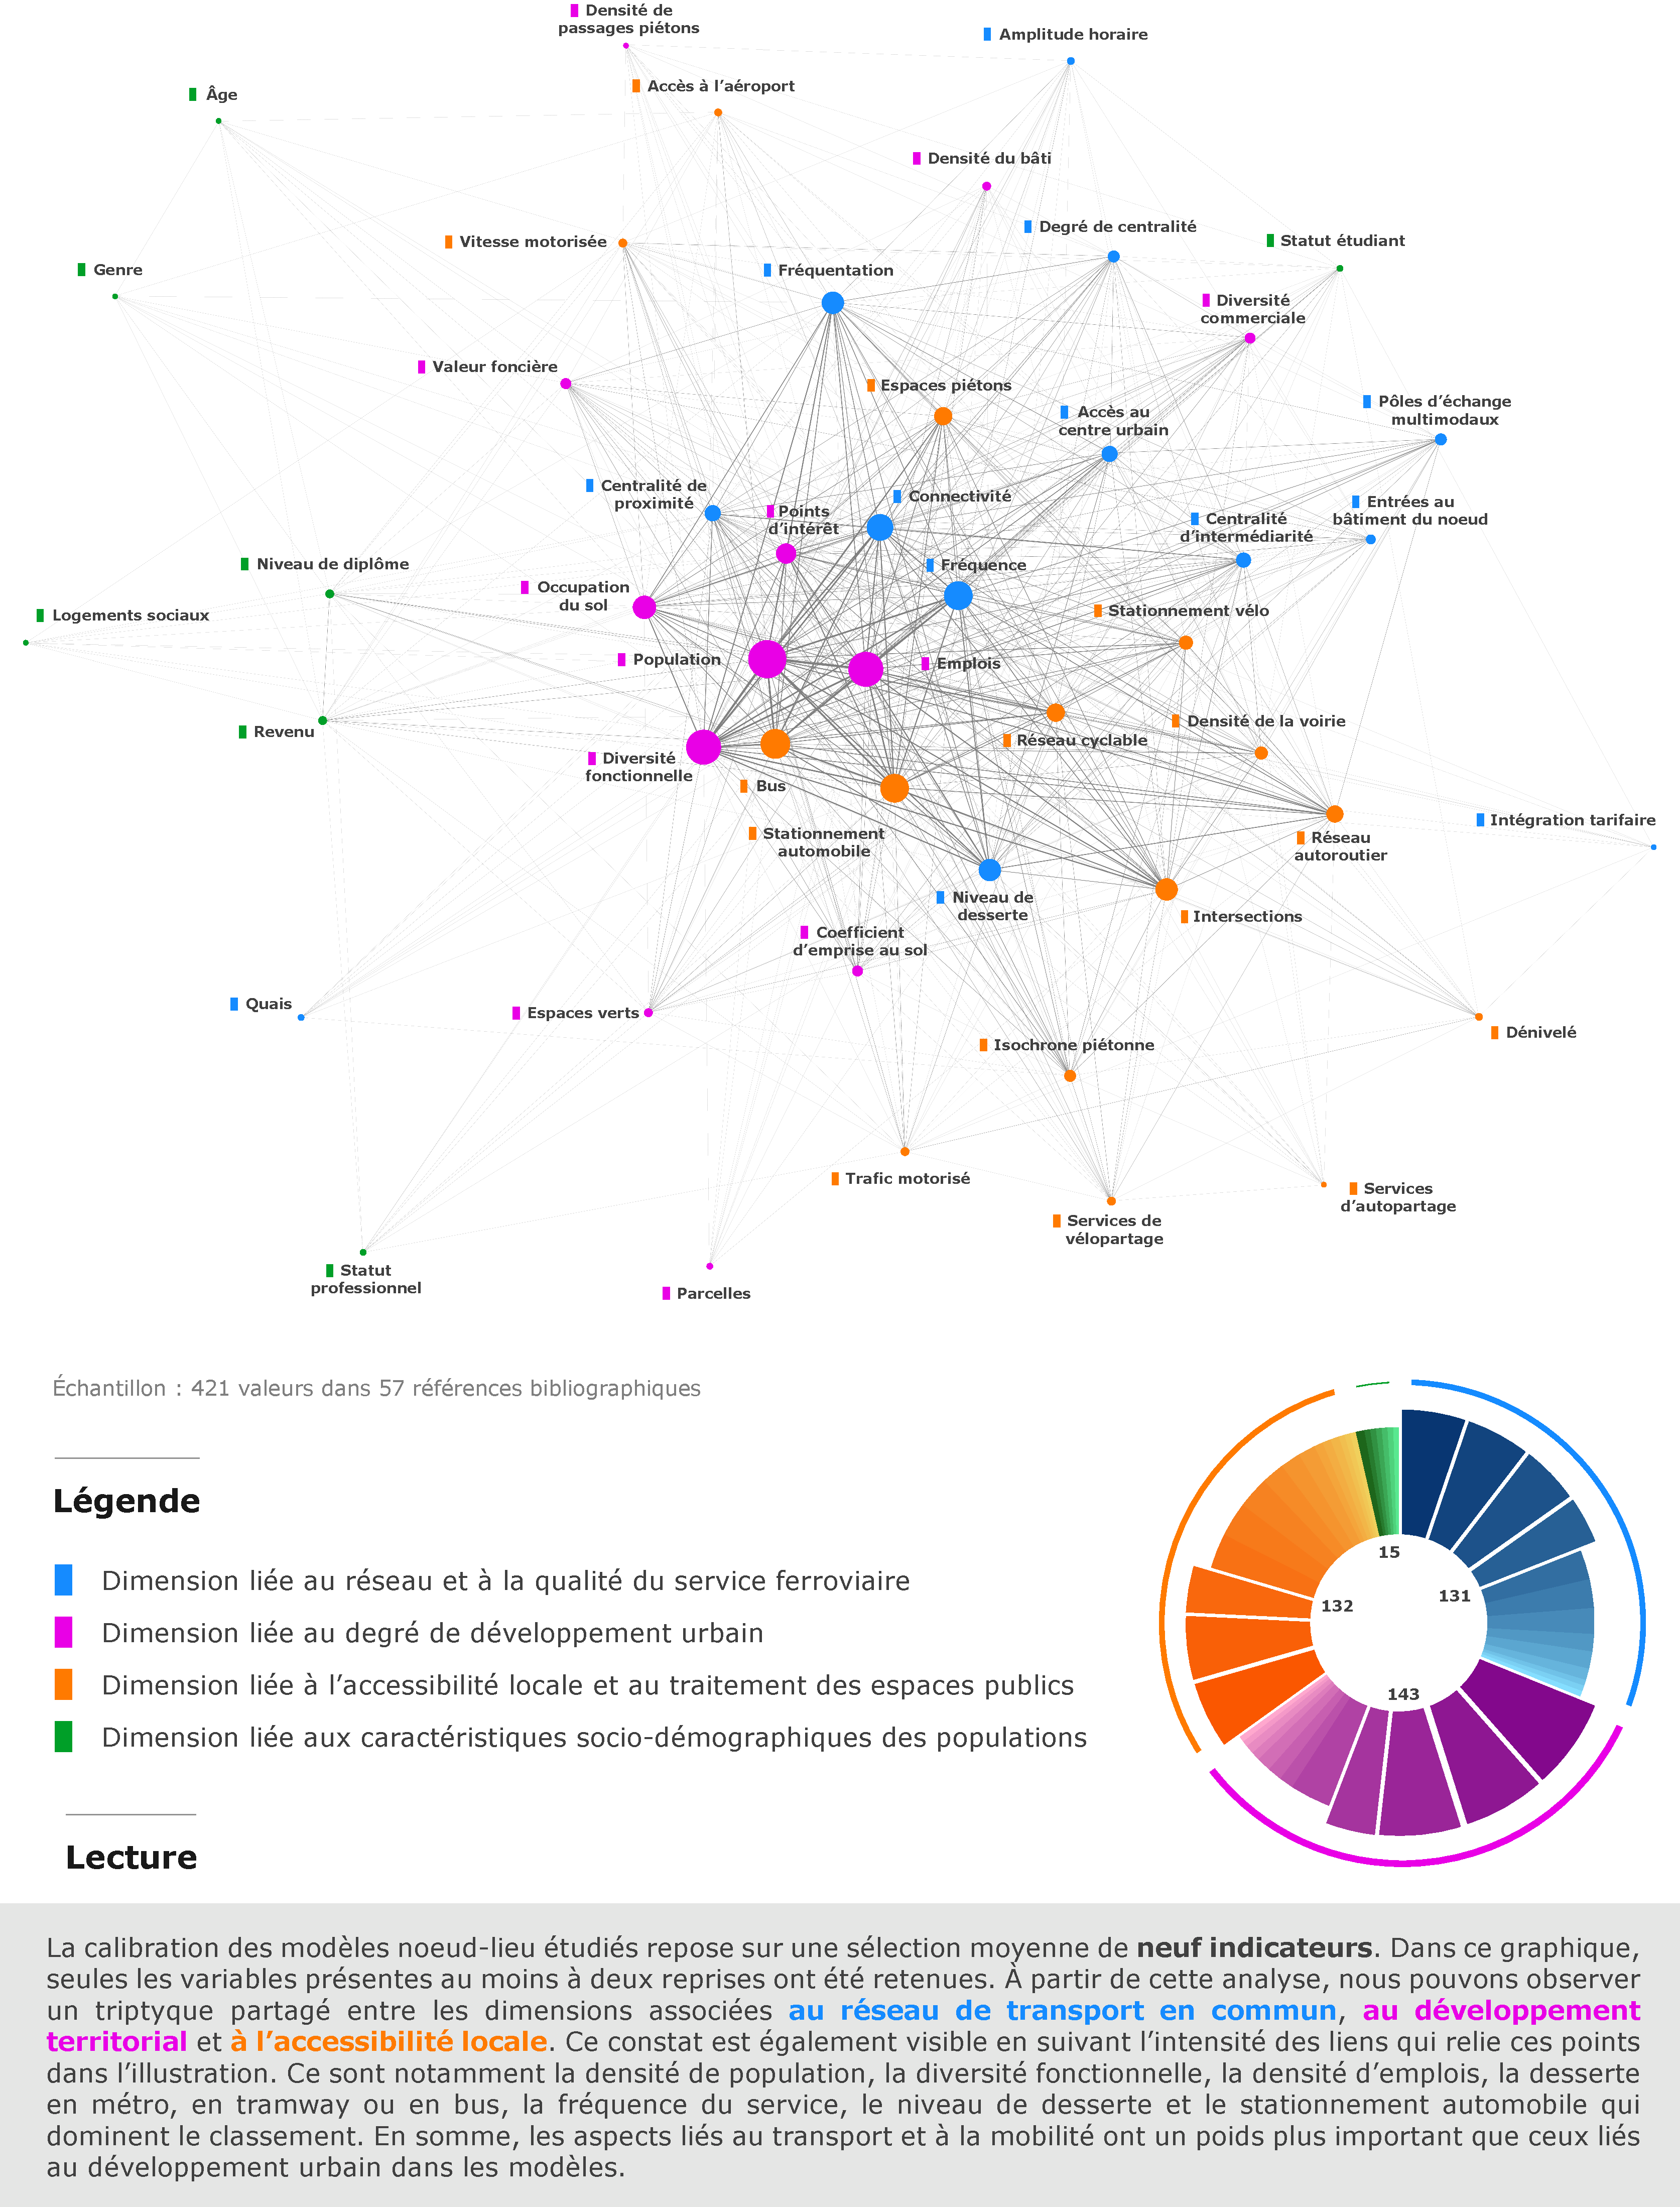
\includegraphics[width=1\columnwidth]{src/Figures/Chap-6/FR_NPART_Litterature_indicateurs.pdf}}
        \vspace{5pt}
        \begin{flushleft}\scriptsize{
        Note~: les indicateurs utilisés dans une même étude sont reliés par des liens. L'épaisseur des liens reflète donc la fréquence d'une utilisation conjointe des indicateurs.
        }\end{flushleft}
        \begin{flushright}\scriptsize{
        Réalisation~: \textcolor{blue}{Dylan Moinse (2024)}
        \\
        Auteur·rice·s~: projet de recherche \acrshort{NPART}
        }\end{flushright}
    \end{figure}

    % Indicateurs recensés
Parmi les 57 études détaillant les paramètres définis dans l'élaboration de leur \acrshort{NPM}, nous avons identifié 49 indicateurs mobilisés ayant au moins 2 occurrences, que nous avons classés en 4 dimensions~: \Guillemets{service de transport en commun}, \Guillemets{développement urbain}, \Guillemets{accessibilité locale} et \Guillemets{caractéristiques socio-démographiques des populations}. En tout, 421 occurrences d’indicateurs ont été recensées, ce qui correspond à une sélection moyenne de 9 indicateurs par modèle étudié. Plus précisément, comme le montre le \hyperref[fig-chap6:litterature-indicateurs]{schéma~\ref{fig-chap6:litterature-indicateurs}} (page~\pageref{fig-chap6:litterature-indicateurs}), 13 variables sont présentes dans la première dimension, représentant 131 occurrences~; 12 variables dans la seconde dimension, représentant 143 occurrences~; 15 variables dans la troisième dimension, représentant 132 occurrences~; et 7 variables dans la dernière dimension, représentant 15 occurrences. Cette analyse révèle une répartition tripartite des indicateurs entre les dimensions associées à l'offre de transport en commun, au degré de développement urbain, et à la qualité des espaces publics combinée à l'accessibilité locale. Ce constat rejoint l'analyse de \textcolor{blue}{\textcite[42]{lyu_developing_2016}}\index{Lyu, Guowei|pagebf}\index{Bertolini, Luca|pagebf}\index{Pfeffer, Karin|pagebf} qui ont identifié, sur la base d'une revue systématique de la littérature, la présence de 94 indicateurs, dont 24 se concentrant sur l'aspect lié au \Guillemets{transport}, 53 sur le \Guillemets{développement urbain} et 17 sur le \Guillemets{\textsl{\gls{design}}}.%%Rédigé%%

    % Critères principaux littérature
Les critères les plus fréquemment utilisés incluent la densité de population (31 occurrences) et d'emploi (28 occurrences), la diversité fonctionnelle (28 occurrences), la desserte en transport en commun urbain (23 occurrences), la fréquence du service de mobilité (22 occurrences), le niveau de desserte en termes de stations accessibles dans une distance-temps donnée (22 occurrences), l'offre en stationnement automobile (22 occurrences) et la connectivité du réseau exprimée en nombre de directions accessibles depuis une station (20 occurrences). En examinant l'intensité des liens entre ces indicateurs dans l'\hyperref[fig-chap6:litterature-indicateurs]{illustration~\ref{fig-chap6:litterature-indicateurs}} (page~\pageref{fig-chap6:litterature-indicateurs}), nous observons que les connexions les plus fréquentes se trouvent entre d'une part, la densité de population et d'autre part, la densité d'emploi (26 liens), la diversité fonctionnelle (23 liens), le stationnement automobile (21 liens) et la présence de systèmes de transport en commun urbain (21 liens), mais également entre la densité d'emploi et la diversité fonctionnelle (20 liens).%%Rédigé%%

    % Recommandations de recherche et transition
Malgré l'identification d'une multitude de modèles réadaptés aux objectifs de recherche et aux contextes géographiques spécifiques, \textcolor{blue}{\textcite[394]{ibrahim_planning_2022}}\index{Ibrahim, Sara|pagebf}\index{Ayad, Hany|pagebf}\index{Saadallah, Dina|pagebf} estiment que la littérature présente une lacune en matière de mesure quantitative du potentiel \acrshort{TOD}. Par ailleurs, \textcolor{blue}{\textcite[10-12]{olaru_place_2019}}\index{Olaru, Doina|pagebf}\index{Moncrieff, Simon|pagebf}\index{McCarney, Gary|pagebf}\index{Sun, Yuchao|pagebf}\index{Reed, Tristan|pagebf}\index{Pattison, Cate|pagebf}\index{Smith, Brett|pagebf}\index{Biermann, Sharon|pagebf} recommandent d'intégrer les solutions de mobilité liées aux \Guillemets{premiers et derniers kilomètres}, qui n'ont pas reçu suffisamment d'attention dans les modèles \acrshort{NPM} existants. Iels suggèrent également d'élargir le périmètre d'analyse à l'échelle d'un quartier de gare élargi ou d'une \Guillemets{aire secondaire}, comme le mentionnent \textcolor{blue}{\textcite[280]{li_transit_2019}}\index{Li, Zekun|pagebf}\index{Han, Zixuan|pagebf}\index{Xin, Jing|pagebf}\index{Luo, Xin|pagebf}\index{Su, Shiliang|pagebf}\index{Weng, Min|pagebf}. De leur côté, \textcolor{blue}{\textcite[80]{robillard_transit-oriented_2024}}\index{Robillard, Arianne|pagebf}\index{Boisjoly, Geneviève|pagebf}\index{Lierop, Dea van|pagebf} ainsi que \textcolor{blue}{\textcite[120]{nigro_land_2019}}\index{Nigro, Antonio|pagebf}\index{Bertolini, Luca|pagebf}\index{Moccia, Francesco Domenico|pagebf} soulignent l'importance de distinguer l'environnement piétonnier de l'environnement cyclable autour des gares, la littérature ayant tendance à négliger ce dernier aspect dans le contexte du modèle et du \acrshort{TOD} plus largement. En suivant ces recommandations, ainsi que celles de \textcolor{blue}{\textcite[9]{motieyan_development_2018}}\index{Motieyan, Hamid|pagebf}\index{Mesgari, Mohammad Saadi|pagebf} qui proposent de développer un modèle prenant en considération les dynamiques spatiales et temporelles, nous avons élaboré un modèle \acrshort{NPM} enrichi des suggestions issues des études antérieures, tout en recentrant notre recherche principale. Nous avons donc opté pour le calcul d'un modèle étendu, visant à couvrir le réseau ferroviaire complet, afin de maintenir une cohérence comme le recommandent \textcolor{blue}{\autocite[58]{chorus_application_2011}}\index{Chorus, Paul|pagebf}\index{Bertolini, Luca|pagebf}, et sur une large échelle régionale, conformément aux recommandations de \textcolor{blue}{\textcite[643]{wei_classifying_2023}}\index{Wei, Sheng|pagebf}\index{Wang, Lei|pagebf}. Ces préoccupations exprimées à travers la littérature constituent le sujet de la section suivante, dans laquelle nous exposons la grille d'indicateurs définie, avec l'objectif d'étendre et d'ajuster ce modèle avancé à notre problématique de recherche.%%Rédigé%%

     % ___________________________________________
    % 6.2.
    \newpage
    \needspace{1\baselineskip} % Réserve de l'espace
    \sectionheader{Grille d'indicateurs synthétiques intégrés dans la modélisation}
\section{Sélection des indicateurs synthétiques quantifiant et caractérisant les quatre dimensions de la modélisation
    \label{chap6:selection-indicateurs}
    }

    % Introduction
L'exploration de la littérature scientifique concernant le \acrshort{NPM} appuie comment cette approche quantitative s'affine à mesure que les recherches progressent. Ce cadre technique, dont l'objectif principal est de classifier les nœuds et leur environnement afin de déceler un potentiel \acrshort{TOD}, ne cesse de se perfectionner en intégrant progressivement de nouvelles dimensions liées au concept d'aménagement, enrichi par des connaissances toujours plus approfondies. Même si de nouveaux indicateurs sont proposés et intégrés aux modèles développés, notre première section a identifié certaines lacunes intrinsèquement associées à notre \acrshort{RSL} portant sur le \acrshort{B-TOD}. Ces limites concernent, d'une part, la délimitation de périmètres géographiques restreints autour des quartiers de gare, reposant sur une conception réduite de la marche combinée. Cette pratique de recherche soutient par la même occasion l'absence quasi totale de modèles prenant en compte l'apport du vélo et de la micro-mobilité. D'autre part, à une échelle plus large, les terrains géographiques délimités s'avèrent souvent limités à une commune ou à une agglomération. Par ailleurs, l'insuffisance d'études de cas situées en France, malgré la richesse des bases de données ouvertes, nous invite à conduire une telle investigation sur ce territoire, dans le souci de saisir des similitudes ou encore des spécificités nationales ou locales.%%Rédigé%%

    % Innovations
Forts de ce constat, nous avons opté pour une démarche novatrice en choisissant d'examiner un terrain encore inexploré, tout en intégrant les apports les plus récents liés au \acrshort{NPM}. Cela inclut une pluralité d'indicateurs introduits dans les derniers modèles publiés, ainsi que des paramètres originaux se concentrant sur l'intégration encore peu documentée de la mobilité individuelle légère. En d'autres termes, la modélisation que nous avons adoptée repose sur une version revisitée du \acrshort{NPM}, prenant en compte l'apport du vélo et de la micro-mobilité. Cette approche vise à déterminer si des nuances apparaissent en comparaison avec la marche combinée, dans le cadre élargi d'une région.%%Rédigé%%

    % Choix et originalité des dimensions
À cet égard, la définition de notre \acrshort{NPM} tire son originalité de l’intégration de l'ajout de deux dimensions innovantes. D'une part, nous avons veillé à intégrer les liens établis entre l’objet-gare et l’objet urbain prenant la forme d'espaces publics. D'autre part, il s'agit de faire dialoguer ces thématiques avec la demande de mobilité exprimée à travers la fréquentation dynamique des stations de transport en commun. Ainsi, quatre dimensions viennent structurer la modélisation que nous avons choisi de nommer \acrfull{NPART}. Pour chaque indicateur exploité, les \hyperref[annexes:npart-node]{annexes~\ref{annexes:npart-node}, \ref{annexes:npart-place-pi}, \ref{annexes:npart-place-ci}, \ref{annexes:npart-accessibility-pi} et~\ref{annexes:npart-accessibility-ci}} (pages~\pageref{annexes:npart-node}, \pageref{annexes:npart-place-pi}, \pageref{annexes:npart-place-ci}, \pageref{annexes:npart-accessibility-pi} et~\pageref{annexes:npart-accessibility-ci}) présentent des informations sur leur distribution statistique, dans le but d'alimenter la démarche typologique à venir, en faisant ressortir la variance qui permet de différencier les gares.%%Rédigé%%

    % Détails dimensions + annonce du plan
Premièrement, les deux composantes traditionnelles du \acrshort{NPM}, structurent notre modèle~: (i) la configuration et la qualité de service du réseau ferroviaire représentent l'axe \textsl{node} du concept d’aménagement (voir la \hyperref[chap6:methodologie-indicateurs-node]{section \textsl{Transit}}, page~\pageref{chap6:methodologie-indicateurs-node}), (ii) conjuguées avec les agencements territoriaux \textsl{autour} des lieux de connexion ferroviaire, qui correspondent à l'axe \textsl{place} (voir la \hyperref[chap6:methodologie-indicateurs-place]{section \textsl{Development}}, page~\pageref{chap6:methodologie-indicateurs-place}). Deuxièmement, l’élargissement de cette approche géostatistique se traduit par (iii) l'intégration de la qualité des espaces publics et de l’accessibilité locale, qui interrogent le niveau de développement urbain \textsl{connecté} à ces gares et qui composent ainsi l'axe \textsl{accessibility} (voir la \hyperref[chap6:methodologie-indicateurs-accessibility]{section \textsl{Oriented}}, page~\pageref{chap6:methodologie-indicateurs-accessibility}). De plus, (iv) les flux de passager·ère·s sont analysés sous une perspective temporelle et incarnent le dernier axe associé au \textsl{ridership per time} (voir la \hyperref[chap6:methodologie-indicateurs-frequentation]{section \textsl{Demand}}, page~\pageref{chap6:methodologie-indicateurs-frequentation}). Ces quatre dimensions, détaillées dans les sous-sections suivantes, forment ainsi la base de notre modèle \acrshort{NPART}. Ce modèle s’inscrit dans une démarche plus large visant à redéfinir le cadre du \acrshort{M-TOD}, qui constitue l’objet central de cette recherche doctorale.%%Rédigé%%

    % 6.2.1.
    \needspace{1\baselineskip} % Réserve de l'espace
\subsection{Qualité du service ferroviaire (nœud)
    \label{chap6:methodologie-indicateurs-node}
    }

    % Catégories node
La première dimension, relative à la \Guillemets{qualité du service ferroviaire}, se décline en quatre catégories~: le \Guillemets{niveau de service}, la \Guillemets{performance du système}, la \Guillemets{métrique du réseau} sous l'angle des graphes et l'\Guillemets{accessibilité aux centralités} urbaines de Lille et de Paris, comme le présente le \hyperref[table-chap6:indicateurs-node]{tableau~\ref{table-chap6:indicateurs-node}} (page~\pageref{table-chap6:indicateurs-node}). L'objectif de cette première dimension, en conformité avec le \acrshort{NPM} d'origine, est de représenter l'offre ferroviaire désignée par \(N\) dans la région, en interrogeant ses différents aspects structurés autour de seize indicateurs clés. Notons que contrairement aux trois autres dimensions, les valeurs de chacun des indicateurs synthétiques sont similaires pour les quatre types de périmètres géographiques étudiés (\(PI\), \(PB\), \(CI\) et \(CB\)).%%Rédigé%%

    % Justification indicateurs Node
Cette première catégorie, relevant du volet \Guillemets{\textsl{Transit}} du \textsl{Transit-Oriented Development}, vise à évaluer de manière exhaustive la qualité de service offerte par l'infrastructure ferroviaire. Il est établi que la fréquence des réseaux de transport en commun influence considérablement la fréquentation des gares \textcolor{blue}{\autocite[79]{sung_transit-oriented_2011}}\index{Sung, Hyungun|pagebf}\index{Oh, Ju-Taek|pagebf}. De manière similaire, \textcolor{blue}{\textcite[63]{kashfi_effects_2015}}\index{Kashfi, Syeed Anta|pagebf}\index{Bunker, Jonathan~M.|pagebf}\index{Yigitcanlar, Tan|pagebf} soulignent que l'intensité des services et leur amplitude horaire favorisent l'accroissement de leur fréquentation. Dans le cadre de notre modélisation, nous avons donc quantifié le niveau de service en définissant la fréquence des réseaux \acrshort{TGV} et \acrshort{TER} (\(N_{1}\), \(N_{2}\), \(N_{3}\) et \(N_{4}\)), ainsi que l'amplitude horaire (\(N_{5}\) et \(N_{6}\)). Nous avons également pris en compte la performance du système, incluant la vitesse commerciale (\(N_{7}\)), qui influe sur le volume de voyageur·se·s \textcolor{blue}{\autocite[149-201]{vuchic_urban_2007}}\index{Vuchic, Vukan~R.|pagebf} et le nombre de directions desservies (\(N_{8}\)), identifié comme un indicateur déterminant dans divers modèles \acrshort{NPM} pour la fréquentation des nœuds \textcolor{blue}{\autocite[9]{cao_coordination_2020}}\index{Cao, Zhejing|pagebf}\index{Asakura, Yasuo|pagebf}\index{Tan, Zongbo|pagebf}. Nous avons exploré la structure du réseau à travers l'analyse de graphes, en évaluant des aspects tels que le degré de centralité (\(N_{9}\)) et la centralité de proximité (\(N_{11}\)), qui, d'après \textcolor{blue}{\textcite[14]{shi_exploring_2018}}\index{Shi, Zhuangbin|pagebf}\index{Zhang, Ning|pagebf}\index{Liu, Yang,|pagebf}\index{Xu, Wei|pagebf}, jouent un rôle essentiel dans l'attractivité des gares, ainsi que la centralité d'intermédiarité (\(N_{10}\)), associée à une augmentation du nombre de passager·ère·s \textcolor{blue}{\autocite[339]{jang_influence_2022}}\index{Jang, Seongman|pagebf}\index{An, Youngsoo|pagebf}. Enfin, la dernière branche examine l'accessibilité aux centralités urbaines, en se concentrant sur les distances vers les pôles urbains (\(N_{13}\), \(N_{14}\), \(N_{15}\) et \(N_{16}\)), inversement corrélées à l'attractivité des gares \textcolor{blue}{\autocites[8]{liu_how_2016}[241]{kuby_factors_2004}}\index{Liu, Chao|pagebf}\index{Erdoğan, Sevgi|pagebf}\index{Ma, Ting|pagebf}\index{Ducca, Frederick~W.|pagebf}\index{Kuby, Michael|pagebf}\index{Barranda, Anthony|pagebf}\index{Upchurch, Christopher|pagebf}.%%Rédigé%%

    % Tableau grille d'indicateurs (node)
% Tableau grille d'indicateurs (node)
%%Rédigé%%
    \begin{table}[h!]
    \centering
    \renewcommand{\arraystretch}{1.5}
    \resizebox{\columnwidth}{!}{
    \begin{tabular}{p{0.43\columnwidth}p{0.08\columnwidth}p{0.49\columnwidth}}
        %\hline
    \rule{0pt}{15pt} \small{\textbf{\textcolor{blue}{Catégorie}}} & \small{\textbf{\textcolor{blue}{ID}}} & \small{\textbf{\textcolor{blue}{Indicateur}}}\\
        \hline
    \multirow{8.5}{*}{\textbf{Niveau de service}} & \small{\multirow{1.5}{*}{\(N_{1}\)}} & \small{Fréquence quotidienne des lignes \acrshort{TGV}, en semaine}\\
& \small{\multirow{1.5}{*}{\(N_{2}\)}} & \small{Fréquence quotidienne des lignes \acrshort{TGV}, un samedi et dimanche}\\
& \small{\multirow{1.5}{*}{\(N_{3}\)}} & \small{Fréquence quotidienne des lignes \acrshort{TER}, en semaine}\\
& \small{\multirow{1.5}{*}{\(N_{4}\)}} & \small{Fréquence quotidienne des lignes \acrshort{TER}, un samedi et dimanche}\\
& \small{\(N_{5}\)} & \small{Amplitude horaire, en semaine}\\
& \small{\(N_{6}\)} & \small{Amplitude horaire, un samedi et dimanche}\\
        \hdashline
    \multirow{2}{*}{\textbf{Performance du système}} & \small{\(N_{7}\)} & \small{Vitesse commerciale}\\
& \small{\(N_{8}\)} & \small{Nombre de directions desservies}\\
        \hdashline
    \multirow{3}{*}{\textbf{Métrique du réseau}} & \small{\(N_{9}\)} & \small{Degré de centralité}\\
& \small{\(N_{10}\)} & \small{Centralité d'intermédiarité}\\
& \small{\(N_{11}\)} & \small{Centralité de proximité}\\
        \hdashline
    \multirow{8}{*}{\textbf{Accessibilité aux centralités}} & \small{\multirow{1.5}{*}{\(N_{12}\)}} & \small{Nombre de stations accessibles en une heure}\\
& \small{\multirow{1.5}{*}{\(N_{13}\)}} & \small{Nombre de stations pour accéder au centre urbain de Lille (pôle Euralille)}\\
& \small{\multirow{1.5}{*}{\(N_{14}\)}} & \small{Temps de trajet pour accéder au centre urbain de Lille (pôle Euralille)}\\
& \small{\multirow{1.5}{*}{\(N_{15}\)}} & \small{Nombre de stations pour accéder au centre urbain de Paris (pôle Châtelet)}\\
& \small{\multirow{1.5}{*}{\(N_{16}\)}} & \small{Nombre de stations pour accéder au centre urbain de Paris (pôle Châtelet)}\\
        \hline
        \end{tabular}}
    \caption{Grille d'indicateurs regroupés dans la dimension associée à la \Guillemets{qualité du service ferroviaire} (nœud).}
    \label{table-chap6:indicateurs-node}
        \vspace{5pt}
        \begin{flushleft}\scriptsize{
        \textcolor{blue}{Lecture~:} seize indicateurs sont regroupés dans la dimension \(N\). 
        }\end{flushleft}
        \begin{flushright}\scriptsize{
        Réalisation~: \textcolor{blue}{Dylan Moinse (2024)}
        \\
        Auteur·rice·s~: projet de recherche \acrshort{NPART}
        }\end{flushright}
        \end{table}%%Rédigé%%

    % 6.2.1.1.
    \needspace{1\baselineskip} % Réserve de l'espace
\subsubsection*{Niveau de service du réseau \(N_{1} - N_{6}\)
    \label{chap6:indicateurs-node-niveau-service}
    }

    % Catégorie "niveau de service"
Concernant le \Guillemets{niveau de service} du réseau de transport en commun interurbain, nous avons jugé pertinent d'intégrer six facteurs abordant deux aspects distincts\footnote{
    Pour ce faire, nous avons utilisé les jeux de données statiques \acrfull{GTFS} fournis par la \textcolor{blue}{\textcite{sncf_reseau_2024}}. Le premier jeu de données couvre la période du 18 mars au 12 avril 2024 pour le \acrshort{TGV}, tandis que le second s'étend du 23 mars au 21 avril 2024. Nous avons ainsi déterminé, sur la base de représentations par graphe, une fréquence moyenne des lignes \acrshort{TGV} en semaine (sur 20 jours) et le week-end (sur 7 jours), ainsi que des lignes \acrshort{TER} en semaine (sur 25 jours) et le week-end (sur 10 jours), en calculant également une amplitude horaire moyenne respectivement sur 5 jours et sur 2 jours. L'unité de mesure utilisée est le nombre de trains par jour pour la fréquence et le nombre d'heures et de minutes pendant lesquelles les lignes sont en service quotidiennement, pour l'amplitude horaire.
}. Le premier aspect consiste à examiner la fréquence quotidienne des différentes lignes en différenciant les types de système~: d'une part, les lignes \acrshort{TGV} (\(N_{1}\) et \(N_{2}\)) et, d'autre part, les lignes régionales de type \acrshort{TER} et \acrfull{TERGV} (\(N_{3}\) et \(N_{4}\)). Cette analyse est menée en tenant compte des jours de la semaine, en distinguant les jours ouvrables des week-ends. Le second aspect concerne l'amplitude horaire des services de mobilité, en semaine (\(N_{5}\)) et le week-end (\(N_{6}\)).%%Rédigé%%

    % Statistiques descriptives
La fréquence moyenne des 318 gares du réseau \acrshort{TGV} est de 0,76 train par jour de semaine et de 0,65 train les samedis et dimanches. Cependant, cette moyenne atteint respectivement 14,29 et 12,23 trains quotidiens si nous considérons uniquement les 17 gares desservies par le réseau à grande vitesse. Pour le réseau ferroviaire régional, la fréquence moyenne des 318 gares est de 31,50 trains par jour de semaine et de 13,30 trains par jour de week-end. En ce qui concerne les horaires d'ouverture, les lignes ferroviaires sont généralement en service 14 heures et 47 minutes par jour de semaine et 12 heures et 36 minutes par jour de week-end\footnote{
    \textsl{Fréquence} (\(N_{1} - N_{4}\))~: en guise d'illustration, le pôle d'échange multimodal \textsl{Euraflandres} se distingue avec une fréquence de 91,95 \acrshort{TGV} par jour ouvrable et de 82,57 \acrshort{TGV} par jour de week-end, et respectivement de 512,92 et de 228,30 \acrshort{TER} et \acrshort{TERGV} quotidiens.
    \\
    \textsl{Amplitude horaire} (\(N_{5} - N_{6}\))~: la gare d'Amiens se classe en tête avec une durée de service respective de 19 heures et 31 minutes et de 18 heures et 49 minutes.
}.%%Rédigé%%

    % 6.2.1.2.
    \needspace{1\baselineskip} % Réserve de l'espace
\subsubsection*{Performance du système \(N_{7} - N_{8}\)
    \label{chap6:indicateurs-node-performance}
    }

    % Catégorie "performance"
La \Guillemets{performance du système} se structure autour de deux indicateurs principaux~: la vitesse commerciale du réseau ferroviaire (\(N_{7}\)) et le nombre de directions desservies dans les gares examinées (\(N_{8}\))\footnote{
    Pour ces deux variables, nous avons choisi le mardi 19 mars 2024 afin d'agréger l'ensemble des vitesses enregistrées et des directions proposées dans chaque gare, à l'aide de représentations par graphe. Pour le calcul des vitesses, nous avons déterminé la vitesse moyenne de chaque ligne ferroviaire desservant les gares, puis retenu la vitesse moyenne la plus élevée pour chaque gare.
}. Ainsi, la vitesse moyenne dans les 318 gares est de 69,68 kilomètres par heure, s'élevant à 137,97 kilomètres par heure pour les 17 gares desservies par le réseau \acrshort{TGV}, et à 65,83 kilomètres heure pour les gares exclusivement connectées au réseau \acrshort{TER}. En ce qui concerne le nombre de directions proposées par les gares, la moyenne est de 3,35 destinations différentes par gare\footnote{
    \textsl{Vitesse commerciale et nombre de directions} (\(N_{7} - N_{8}\))~: la gare bénéficiant de la ligne la plus rapide et du plus grand nombre de directions proposées est le \textsl{hub Euraflandres}, avec une vitesse moyenne de 236,75 kilomètres par heure et 48 destinations différentes.
}.%%Rédigé%%

    % 6.2.1.3.
    \needspace{1\baselineskip} % Réserve de l'espace
\subsubsection*{Métrique du réseau \(N_{9} - N_{11}\)
    \label{chap6:indicateurs-node-metrique}
    }

    % Catégorie "métrique"
La \Guillemets{métrique du réseau} s'articule quant à elle autour de trois indicateurs synthétiques~: le degré de centralité (\(N_{9}\)), la centralité d'intermédiarité (\(N_{10}\)) et la centralité de proximité (\(N_{11}\))\footnote{
    Le degré de centralité (\textsl{degree centrality}) mesure le nombre de connexions directes qu'un nœud a avec d'autres nœuds dans un réseau. Plus un nœud a de connexions, plus son degré de centralité est élevé. Par connexions directes, nous entendons ici le nombre de gares atteintes par des services ferroviaires, sans correspondance, depuis la gare de départ.
    \\
    La centralité d'intermédiarité (\textsl{betweenness centrality}) quantifie le nombre de fois qu'un nœud apparaît dans les plus courts chemins entre d'autres nœuds. Un nœud avec une centralité d'intermédiarité élevée joue un rôle crucial de médiateur dans un réseau.
    \\
    La centralité de proximité (\textsl{closeness centrality}) mesure à quel point un nœud est proche de tous les autres nœuds d'un réseau. Elle est définie comme l'inverse de la somme des distances les plus courtes entre un nœud et tous les autres nœuds.
}. Ces trois principales mesures issues de la théorie des graphes permettent d'évaluer la position stratégique des gares dans le réseau ferroviaire\footnote{
    Pour cette analyse, nous avons également retenu le mardi 19 mars 2024, en tant que jour ouvrable de base, afin d'étudier l'ensemble des flux ferroviaires prévus ce jour-là.
}. Les moyennes correspondant r
espectivement au degré de centralité, à la centralité d'intermédiarité et à la centralité de proximité des 318 gares de la région s'établissent respectivement à 0,001~; 0,092 et à 0,001\footnote{
    \textsl{Position dans le réseau} (\(N_{9} - N_{11}\))~: la gare présentant les valeurs métriques les plus élevées est, une fois de plus, le pôle \textsl{Euraflandres}, avec un degré de centralité de 0,008 ainsi que des centralités d'intermédiarité de 0,246 et de proximité de 0,102.
}.%%Rédigé%%

    % 6.2.1.4.
    \needspace{1\baselineskip} % Réserve de l'espace
\subsubsection*{Accessibilité aux centralités urbaines \(N_{12} - N_{16}\)
    \label{chap6:indicateurs-node-accessibilite-centralites}
    }

    % Catégorie "accessibilité aux centralités"
Le dernier aspect correspond à l'\Guillemets{accessibilité aux centralités} urbaines et regroupe cinq indicateurs~: le nombre de stations accessibles en une heure de trajet (\(N_{12}\)), le nombre de stations et la distance-temps nécessaires pour accéder respectivement au pôle Euralille, situé au centre de Lille (\(N_{13}\) et \(N_{14}\)), et au pôle Châtelet, situé au centre de Paris (\(N_{15}\) et \(N_{16}\)). Cette dernière catégorie étant consacrée à la distance aux pôles urbains attractifs, les valeurs obtenues, que ce soit pour \(N_{13}\), \(N_{14}\), \(N_{15}\) et \(N_{16}\), sont inversées dans la modélisation, de façon à classer les nœuds en fonction de leur proximité à Lille et à Paris\footnote{
    Le budget temps attribué a été déterminé en se basant sur l'enquête publique menée par le \textcolor{blue}{\textcite{ministere_de_la_transition_ecologique_et_de_la_cohesion_des_territoires_mobilite_2023}}, qui indique qu'un déplacement \Guillemets{local ou longue distance} réalisé en France dure en moyenne 41 minutes en 2019. Cette donnée a été croisée avec notre matériau empirique, tendant vers 1 heure de déplacement en \acrshort{TGV} et en \acrshort{TER} dans la région. De la même manière que précédemment, nous avons retenu le mardi 19 mars 2024, entre 5h00 et 23h00, pour étudier l'accessibilité aux autres gares du réseau national. Concernant l'accessibilité aux centralités urbaines d'Euralille et de Châtelet, nous avons analysé les flux du 18 mars au 24 mars 2024, soit une semaine complète, puis conservé les valeurs les plus faibles pour chaque gare.
}.%%Rédigé%%

    % Statistiques descriptives gares en 1 heure
Pour l'accessibilité aux autres gares dans un temps donné, le nombre moyen de gares accessibles en 1 heure est de l'ordre de 1,99, contre 4,58 gares pour les 17 gares reliées au réseau à grande vitesse. Pour l'accès au centre urbain de Lille, le nombre moyen de gares pour y accéder est de 4,63 gares, avec une distance-temps moyenne de 1 heure et 10 minutes. L'accessibilité au centre urbain de Paris montre une moyenne de 5,83 gares pour y accéder, avec une distance-temps moyenne de 1 heure et 50 minutes. Neuf gares de la région ont un accès direct en train, sans arrêt intermédiaire, bien que nécessitant une rupture de charge à la Gare du Nord pour atteindre le centre urbain de Paris. Parmi ces gares, seules deux sont desservies par le \acrshort{TGV}~: celles d'Arras et d'\textsl{Euraflandres}\footnote{
    \textsl{Accès aux autres stations} (\(N_{12}\))~: le \textsl{hub Euraflandres} reste en tête du classement avec une moyenne de 15,44 gares accessibles en une heure.
    \\
    \textsl{Accès à Lille} (\(N_{13} - N_{14}\))~: en excluant le pôle d'échange multimodal concerné pour les indicateurs relatifs aux distances à Euralille, 24 gares ont une liaison directe sans arrêt intermédiaire jusqu'au centre urbain de Lille. En dehors des gares de la \acrfull{MEL}, les gares d'importance régionale telles que celles d'Arras, Calais-Fréthun, Douai, Dunkerque, Orchies, Templeuve, TGV Haute Picardie et de Valenciennes figurent parmi ces connexions directes. De plus, 37 gares sont connectées à moins de 20 minutes d'Euralille, principalement au sein de la \acrshort{MEL}, à l'exception des gares de Douai, Landas, Libercourt, Nieppe, Nomain, Orchies, Ostricourt et de Phalempin.
    \\
    \textsl{Accès à Paris} (\(N_{15} - N_{16}\))~: en termes de distance-temps de trajet, la gare d'Orry-la-Ville-Coye enregistre le score le plus court avec 28 minutes, suivie de Chantilly-Gouvieux avec 33 minutes et de Creil avec 36 minutes, ces trois gares étant frontalières de l'Île-de-France et connectées à la ligne D du \acrfull{RER}.
}.%%Rédigé%%

    % 6.2.1.5.
    \needspace{1\baselineskip} % Réserve de l'espace
\subsubsection*{Originalité de la dimension en rapport avec le nœud
    \label{chap6:indicateurs-node-originalite}
    }

    % Introduction
En proposant ces seize indicateurs pour la dimension relative à l'offre ferroviaire, notre modèle s'inspire de modèles \acrshort{NPM} antérieurs tout en les affinant. Cette première dimension, portant sur l'infrastructure et le service de mobilité régionale, s'efforce d'apporter une réponse aux trois défis majeurs auxquels se heurte le développement des modèles d'accessibilité par les transports en commun~: la performance du système, la configuration du réseau de transport public ainsi que l'accès aux diverses destinations \textcolor{blue}{\autocite[744]{malekzadeh_review_2020}}\index{Malekzadeh, Ali|pagebf}\index{Chung, Edward|pagebf}.%%Rédigé%%

    % Performance du système 1
Du point de vue de la qualité du service ferroviaire, nous avons d'abord cherché à élargir le spectre temporel de l'analyse statistique en projetant des graphes plus complexes qui dépassent la simple considération d'un intervalle horaire unique ou d'une seule journée, à l'instar de la quasi-totalité des études recensées. En effet, la plupart d'entre elles calculent ces variables à partir d'une journée type, généralement un mardi, voire d'une seule tranche horaire, le plus souvent en heure de pointe. Bien que la fréquence soit parmi les indicateurs les plus mobilisés, l'originalité de notre modèle réside dans la distinction entre les différents systèmes de transport en commun, ainsi que la séparation entre les jours de semaine et les jours de fin de semaine. Ce souci de différenciation évoque les modèles développés par \textcolor{blue}{\textcite[149]{ivan_evaluation_2012}}\index{Ivan, Igor|pagebf}\index{Boruta, Tomáš|pagebf}\index{Horak, Jiri|pagebf} qui ont isolé la fréquence des trains de celle des trains de banlieue, des tramways et des bus, ainsi que par \textcolor{blue}{\textcite[117]{nigro_land_2019}}\index{Nigro, Antonio|pagebf}\index{Bertolini, Luca|pagebf}\index{Moccia, Francesco Domenico|pagebf}, dont la fréquence a été évaluée selon les périodes de travail et de vacances.%%Rédigé%%

    % Performance du système 2
De même, le nombre de stations accessibles en une distance-temps donnée a été largement incorporé dans les modèles \acrshort{NPM}. Cependant, nous avons choisi d'élargir l'intervalle temporel, régulièrement limité à vingt minutes et qui nous paraît peu adapté à un système ferroviaire à l'échelle régionale. Concernant l'amplitude horaire entre le premier et le dernier train en service, seul le modèle issu de la thèse de doctorat de \textcolor{blue}{Freke} \textcolor{blue}{\textcite[132]{caset_planning_2019}}\index{Caset, Freke|pagebf} considère cet aspect. La question de la vitesse commerciale des trains a été abordée en améliorant les travaux de \textcolor{blue}{\textcite[271]{debrezion_modelling_2009}}\index{Debrezion, Ghebreegziabiher|pagebf}\index{Pels, Eric|pagebf}\index{Rietveld, Piet|pagebf} et de \textcolor{blue}{\textcite[6]{zheng_classifying_2023}}\index{Zheng, Lingwei|pagebf}\index{Austwick, Martin Zaltz|pagebf}, qui se sont intéressé·e·s à la vitesse théorique des trains. À cette fin, nous avons choisi de calculer la vitesse moyenne utile en exploitation sur le réseau commercial, plutôt que d’utiliser la vitesse théorique.%%Rédigé%%

    % Forme du réseau
Si la qualité du service ferroviaire est généralement bien prise en compte dans les modèles antérieurs, il apparaît que les mesures relatives à la configuration du réseau sont rarement exploitées de manière adéquate \textcolor{blue}{\autocite[72-74]{papa_accessibility_2015}}\index{Papa, Enrica|pagebf}\index{Bertolini, Luca|pagebf}. Pourtant, comme le démontrent \textcolor{blue}{\textcite[8]{dou_integrating_2021}}\index{Dou, Mingxuan|pagebf}\index{Wang, Yandong|pagebf}\index{Dong, Shihai|pagebf}, qui introduisent cette notion dans une troisième dimension nommée \Guillemets{\textsl{Node-Place-Network}} (NPN), celle-ci se révèle efficace pour mieux appréhender la performance du réseau étudié. Dans cette optique, nous avons intégré trois indicateurs~: le degré de centralité, la centralité d'intermédiarité et la centralité de proximité, lesquels, selon nos observations, n'ont pas encore été analysés conjointement dans les études existantes.%%Rédigé%%

    % 6.2.2.
    \needspace{1\baselineskip} % Réserve de l'espace
\subsection{Degré de développement urbain (lieu)
    \label{chap6:methodologie-indicateurs-place}
    }

    % Catégories place
La deuxième dimension, relative au \Guillemets{degré de développement urbain}, se décline en cinq catégories~: la \Guillemets{densité}, la \Guillemets{diversité fonctionnelle}, les \Guillemets{lieux d'attraction}, la \Guillemets{valeur du terrain} et la \Guillemets{stratification sociale}, comme le présente le \hyperref[table-chap6:indicateurs-place]{tableau~\ref{table-chap6:indicateurs-place}} (page~\pageref{table-chap6:indicateurs-place}). L'objectif de cette catégorie, également en conformité avec le \acrshort{NPM} d'origine, est de mesurer les formes urbaines, les équipements et l'attractivité des territoires, ainsi que le portrait sociologique des populations résidentes, désignés par~\(P\), en examinant ses différents aspects structurés autour de treize indicateurs clés.%%Rédigé%%

    % Tableau grille d'indicateurs (place)
% Tableau grille d'indicateurs (place)
%%Rédigé%%
    \begin{table}[h!]
    \centering
    \renewcommand{\arraystretch}{1.5}
    \resizebox{\columnwidth}{!}{
    \begin{tabular}{p{0.43\columnwidth}p{0.08\columnwidth}p{0.49\columnwidth}}
        %\hline
    \rule{0pt}{15pt} \small{\textbf{\textcolor{blue}{Catégorie}}} & \small{\textbf{\textcolor{blue}{ID}}} & \small{\textbf{\textcolor{blue}{Indicateur}}}\\
        \hline
    \multirow{2}{*}{\textbf{Densité}} & \small{\(P_{1}\)} & \small{Densité de population}\\
& \small{\(P_{2}\)} & \small{Densité d'emploi}\\
        \hdashline
    \multirow{5.5}{*}{\textbf{Diversité fonctionnelle}} & \small{\multirow{1.5}{*}{\(P_{3}\)}} & \small{Usage du sol à dominante résidentielle}\\
& \small{\multirow{1.5}{*}{\(P_{4}\)}} & \small{Usage du sol à dominante commerciale et dédiée aux services publics}\\
& \small{\multirow{1.5}{*}{\(P_{5}\)}} & \small{Usage du sol à dominante de bureaux et industrielle}\\
& \small{\multirow{1}{*}{\(P_{6}\)}} & \small{Usage du sol à dominante d'espaces verts}\\
        \hdashline
    \multirow{3}{*}{\textbf{Lieux d'attraction}} & \small{\(P_{7}\)} & \small{Points d'intérêt (\acrshort{POIs}) de \Guillemets{proximité}}\\
& \small{\multirow{1}{*}{\(P_{8}\)}} & \small{Points d'intérêt (\acrshort{POIs}) \Guillemets{intermédiaires}}\\
& \small{\(P_{9}\)} & \small{Points d'intérêt (\acrshort{POIs}) \Guillemets{supérieurs}}\\
        \hdashline
    \multirow{2.5}{*}{\textbf{Valeur du terrain}} & \small{\(P_{10}\)} & \small{Valeur foncière des biens résidentiels}\\
& \small{\multirow{1.5}{*}{\(P_{11}\)}} & \small{Valeur foncière des biens industriels, commerciaux et de bureaux}\\
        \hdashline
    \multirow{2}{*}{\textbf{Stratification sociale}} & \small{\(P_{12}\)} & \small{Proportion de logements sociaux}\\
& \small{\(P_{13}\)} & \small{Revenu moyen des ménages}\\
        \hline
        \end{tabular}}
    \caption{Grille d'indicateurs regroupés dans la dimension associée au \Guillemets{degré de développement urbain} (lieu).}
    \label{table-chap6:indicateurs-place}
        \vspace{5pt}
        \begin{flushleft}\scriptsize{
        \textcolor{blue}{Lecture~:} treize indicateurs sont regroupés dans la dimension \(P\). 
        }\end{flushleft}
        \begin{flushright}\scriptsize{
        Réalisation~: \textcolor{blue}{Dylan Moinse (2024)}
        \\
        Auteur·rice·s~: projet de recherche \acrshort{NPART}
        }\end{flushright}
        \end{table}%%Rédigé%%

    % 6.2.2.1.
    \needspace{1\baselineskip} % Réserve de l'espace
\subsubsection*{Densité de population et d'emploi \(P_{1} - P_{2}\)
    \label{chap6:indicateurs-place-densite}
    }

    % Catégorie "densité"
Concernant la \Guillemets{densité}, celle-ci concerne à la fois la densité de population (\(P_{1}\)) et la densité d'emploi (\(P_{2}\))\footnote{
    Leur mesure s'est appuyée sur deux jeux de données~: pour le premier indicateur, les données carroyées de la population datant de 2019, prenant la forme de carreaux de 200 mètres de côté et, pour le second indicateur, le \acrfull{Sirene} datant du 2 avril 2024, tous deux provenant de l'\textcolor{blue}{\textcite{insee_grille_2021}}. Nous avons ainsi privilégié le calcul d’un stock de résident·e·s et d’emplois plutôt que leur densité, afin d’obtenir une mesure brute facilement comparable aux autres indicateurs. Cette approche permet d’éviter l’influence de la taille des quartiers de gare et ainsi de limiter les biais dans les résultats. En définitive, cette mesure sur des stocks peut être aisément convertie sous forme de densités.
}. Parmi les 318 quartiers de gare propres à chaque périmètre géographique, la densité moyenne de population, mesurée en habitant·e·s par kilomètre carré, s'établit à 2~999,78 à l'échelle des isochrones piétonnes (\(PI\)), à 1~576,72 pour les zones tampons piétonnes (\(PB\)), à 1~325,03 pour les isochrones cyclables (\(CI\)) et à 773,68 pour les zones tampons cyclables (\(CB\)). Les dix premières positions du classement sont occupées par des quartiers de gare de la \acrshort{MEL}. Concernant la densité d'emploi, les gares de la région enregistrent une moyenne de 418,95 (\(PI\)), 240,03 (\(PB\)), 190,93 (\(CI\)) et de 121,14 (\(CB\)) emplois par kilomètre carré\footnote{
    \textsl{Densité de population} (\(P_{1}\))~: au regard de \(PI\), le pôle \textsl{Euraflandres} présente la densité la plus élevée, à hauteur de 12~931,92 habitant·e·s par kilomètre carré, tandis que les environs des gares de Croix l'Allumette pour \(PB\) (10~486,60) et de Lezennes pour \(CI\) (9~031,43) et \(CB\) (9~018,71) arrivent en tête.
    \\
    \textsl{Densité d'emploi} (\(P_{2}\))~: les aires d'influence des gares bénéficiant des plus grandes densités d'emploi sont celles d'Amiens pour \(PI\) (3~498,30) et de Lille CHR pour \(PB\) (3~423,08), \(CI\) (3~289,78) et \(CB\) (2~804,25).
}.%%Rédigé%%

    % 6.2.2.2.
    \needspace{1\baselineskip} % Réserve de l'espace
\subsubsection*{Diversité fonctionnelle \(P_{3} - P_{6}\)
    \label{chap6:indicateurs-place-diversite}
    }
    
    % Catégorie "diversité fonctionnelle"
Quatre aspects définissent la \Guillemets{diversité fonctionnelle}, à savoir l'usage du sol à dominante résidentielle (\(P_{3}\)), commerciale et liée aux services publics (\(P_{4}\)), de bureaux et industrielle (\(P_{5}\)) ainsi que d'espaces verts (\(P_{6}\))\footnote{
    Ces indicateurs ont pu être déterminés à l'aide du référentiel de l'\acrfull{OCS2D} des cinq départements composant les Hauts-de-France. Ce fichier a été publié en 2021 par la plate-forme géographique collaborative \textcolor{blue}{\textcite{geo2france_occupation_2021}}\index{Géo2France@\textsl{Géo2France}|pagebf}, mise en place par la Région.
}. En général, les quartiers de gare, à l'échelle de \(PI\), présentent une proportion spatiale d'usage résidentiel de l'ordre de 41,95~\%, contre 22,83~\% (\(PB\)), 21,84~\% (\(CI\)) et 12,77~\% (\(CB\)). La proportion surfacique occupée par les commerces et les services publics atteint 6,61~\% (\(PI\)), 4,89~\% (\(PB\)), 5,01~\% (\(CI\)) et 3,31~\% (\(CB\)). S'agissant des activités de bureau et industrielles, la part s'élève à 4,66~\% (\(PI\)), 4,71~\% (\(PB\)), 4,17~\% (\(CI\)) et 3,13~\% (\(CB\)). Enfin, les espaces verts s'étendent sur 1,69~\% de \(PI\), 1,24~\% de \(PB\), 1,26~\% de \(CI\) et 0,86~\% de \(CB\)\footnote{
    \textsl{Usage résidentiel} (\(P_{3}\))~: avec un taux de 77,02~\%, les environs de Nieppe sont les plus résidentiels proportionnellement à l'échelle de l'isochrone piétonnière, suivis de Ronchin à 61,03~\%~; 58,73~\% et 58,20~\% pour les trois autres types de périmètre géographique.
    \\
    \textsl{Commerces et services publics} (\(P_{4}\))~: les quartiers de gare du Poirier Université, avec 32,14~\% pour \(PI\), de Chantilly~–~Gouvieux, avec 33,42~\% et 29,72~\% pour \(PB\) et \(CI\), ainsi que de Pont de Bois, avec 26,76~\% pour \(CI\), figurent en tête.
    \\
    \textsl{Activités de bureau et industrielles} (\(P_{5}\))~: les lieux situés à Mont de Terre, avec 51,13~\%~; 28,79~\% et 23,31~\% pour \(PI\), \(CI\) et \(CB\) et à Nesle, avec 27,53~\% pour \(PB\), dominent cette catégorie.
    \\
    \textsl{Espaces verts} (\(P_{6})\))~: les quartiers de gare les plus verts sont ceux du Quesnoy, avec 31,72~\% (\(PI\)) et de Lens, avec 13,67~\% (\(PB\)), 9,71~\% (\(CI\)) et 9,66~\% (\(CB\)).
}.%%Rédigé%%

    % 6.2.2.3.
    \needspace{1\baselineskip} % Réserve de l'espace
\subsubsection*{Lieux d'attraction \(P_{7} - P_{9}\)
    \label{chap6:indicateurs-place-pois}
    }

    % Catégorie "lieux d'attraction"
Les \Guillemets{lieux d'attraction} sont classés en trois catégories distinctes de \acrfull{POIs}, basées sur leurs fonctions~: les \acrshort{POIs} de \Guillemets{proximité} (\(P_{7}\)), \Guillemets{intermédiaires} (\(P_{8}\)) et \Guillemets{supérieurs} (\(P_{9}\))\footnote{
    Cette segmentation reprend les trois gammes définies par l'\textcolor{blue}{\textcite{insee_base_2021}} dans la \acrfull{BPE}, telle qu'elle est détaillée dans la \hyperref[chap5:potentiel-accessibilite-destinations]{section consacrée aux gains d'accessibilité régionale aux lieux d'intérêt~\ref{chap5:potentiel-accessibilite-destinations}} (page~\pageref{chap5:potentiel-accessibilite-destinations}), du \hyperref[chap5:titre]{chapitre~5~\ref{chap5:titre}} (page~\pageref{chap5:titre}).
}. Premièrement, le nombre moyen de \acrshort{POIs} de \Guillemets{proximité} est de 48,85 équipements pour \(PI\), de 59,67 pour \(PB\), de 115,77 pour \(CI\) et de 134,87 pour \(CB\). Deuxièmement, le nombre moyen de \acrshort{POIs} \Guillemets{intermédiaires} atteint 24,96 (\(PI\)), 29,53 (\(PB\)), 53,79 (\(CI\)) et 60,74 équipements (\(CB\)). Enfin, les \acrshort{POIs} \Guillemets{supérieurs} sont au nombre moyen de 8,51 (\(PI\)), 10,61 (\(PB\)), 20,79 (\(CI\)) et 23,08 (\(CB\))\footnote{
    \textsl{Points d'intérêt} (\(P_{7} - P_{9}\))~: le quartier de gare \textsl{Euraflandres} offre le plus grand nombre de lieux d'attraction, toutes catégories confondues, avec pour \(PI\), \(PB\), \(CI\) et \(CB\) respectivement 888~; 1~134~; 1~747 et 1~778 services locaux, 590~; 701~; 940 et 957 services intermédiaires et 172~; 232~; 391 et 397 services d'intérêt régional.
}.%%Rédigé%%

    % 6.2.2.4.
    \needspace{1\baselineskip} % Réserve de l'espace
\subsubsection*{Valeur du terrain \(P_{10} - P_{11}\)
    \label{chap6:indicateurs-place-foncier}
    }
    
    % Catégorie "valeur du terrain"
La \Guillemets{valeur du terrain} s'intéresse à la valeur foncière attribuée aux propriétés résidentielles (\(P_{10}\)) ainsi qu'aux espaces industriels, commerciaux ou de bureaux (\(P_{11}\))\footnote{
    À cet effet, nous avons consolidé les bases de données annuelles de la Demande Valeur Foncière (DVF), issues de la \textcolor{blue}{\textcite{direction_generale_des_finances_publiques_demandes_2024}}\index{Direction Générale des Finances Publiques@\textsl{Direction Générale des Finances Publiques}|pagebf}, pour la période s'étendant de 2018 à 2023. Cette jointure a permis d'établir une valeur moyenne, exprimée en~\euro~par mètre carré, pour les transactions immobilières réalisées dans chaque quartier de gare durant la période susmentionnée.
}. La valeur foncière des biens résidentiels atteint en moyenne 2~138,47~\euro~par mètre carré dans les quartiers de gares désignés \(PI\), 2~132,18~\euro~pour \(PB\), 2~091,53~\euro~pour \(CI\) et 2~121,75~\euro~pour \(CB\). À propos des propriétés industrielles, commerciales et de bureaux, le prix au mètre carré oscille entre 2~480,26~\euro~(\(PI\)), 2~231,09~\euro~(\(PB\)), 2~072,25~\euro~(\(CI\)) et 1~904,52~\euro~(\(CB\))\footnote{
    \textsl{Valeurs résidentielles} (\(P_{10}\))~: concernant les deux types de périmètres piétons, le territoire de Château-Thierry semble le plus prisé, avec une valeur résidentielle s'élevant à 12~421,96~\euro~(\(PI\)) et 9~905,87~\euro~(\(PB\)). Les quartiers de gare de Pont-Sainte-Maxence et d'\textsl{Euraflandres} se classent respectivement premières pour \(CI\) et \(CB\), avec des valeurs foncières de 6~162,00~\euro~et 6~019,66~\euro~par mètre carré.
    \\
    \textsl{Valeurs industrielles et commerciales} (\(P_{11}\))~: les lieux environnant Pont de Bois se distinguent à ce sujet, enregistrant une valeur foncière moyenne de 153~313,16~\euro~(\(PI\)), 151~861,34~\euro~(\(PB\)), 79~550,92~\euro~(\(CI\)) et de 67~034,70~\euro~par mètre carré (\(CB\)).
}.%%Rédigé%%

    % 6.2.2.5.
    \needspace{1\baselineskip} % Réserve de l'espace
\subsubsection*{Composition socio-économique des territoires \(P_{12} - P_{13}\)
    \label{chap6:indicateurs-place-sociodemographie}
    }
    
    % Catégorie "stratification sociale"
Le dernier volet composant la dimension territoriale traite de la \Guillemets{stratification sociale} des territoires étudiés, en mesurant deux indicateurs portant sur la composition socio-économique des lieux~: la proportion de logements sociaux (\(P_{12}\)) et le revenu annuel des ménages (\(P_{13}\))\footnote{
    Nous avons exploité les données du \acrfull{RPLS} de 2023, fournies par le \textcolor{blue}{\textcite{ministere_de_la_transition_ecologique_et_de_la_cohesion_des_territoires_repertoire_2024}}, pour recenser le parc de logements sociaux en France. Parallèlement, nous avons réutilisé les données carroyées de la population, datant de 2019, de l'\textcolor{blue}{\textcite{insee_grille_2021}} afin de déterminer le revenu moyen de chaque foyer.
}. Nos résultats indiquent que la proportion de logements sociaux varie selon les périmètres géographiques, s'établissant à 6,53~\% dans les \(PI\), 6,82~\% dans les \(PB\), 7,76~\% dans les \(CI\) et 7,56~\% dans les \(CB\). Quant au revenu moyen des ménages, il varie également en fonction des zones étudiées~: 4~105,73~\euro~pour \(PI\), 4~150,90~\euro~pour \(PB\), 4~217,75~\euro~pour \(CI\) et 4~277,94~\euro~pour \(CB\)\footnote{
    \textsl{Logements sociaux} (\(P_{12}\))~: les quartiers de gare de Pont de Bois se distinguent par la plus forte concentration de logements sociaux, avec 38,58~\% (\(PI\)) et 34,37~\% (\(PB\)). En ce qui concerne les quartiers de gare cyclables, Coron de Méricourt affiche les taux les plus élevés, avec 31,06~\% (\(CI\)) et 29,96~\% (\(CB\)).
    \\
    \textsl{Revenus annuels} (\(P_{13}\))~: Les quartiers de gare les plus favorisés sont ceux de Jaux, avec un revenu annuel de 6~321,52~\euro~pour \(PI\), d'Ascq, avec 6~199,81~\euro~pour \(PB\) et d'Ennevelin, avec 6~249,93~\euro~et 6~254,31~\euro~pour les zones cyclables.
}.%%Rédigé%%

    % 6.2.2.6.
    \needspace{1\baselineskip} % Réserve de l'espace
\subsubsection*{Originalité de la dimension en rapport avec le lieu
    \label{chap6:indicateurs-place-originalite}
    }
    
    % Justification littérature 1
Nous avons incorporé et développé des indicateurs, déjà présents dans la plupart des modèles \acrshort{NPM}, tels que la densité de population et des emplois, ainsi que la diversité fonctionnelle des territoires, en complément de nouvelles variables. L'exploitation des \acrshort{POIs} se réfère à des études relativement peu nombreuses qui ont pris en compte ces éléments urbains générateurs de flux \textcolor{blue}{\autocites[82]{robillard_transit-oriented_2024}[2]{zhou_introducing_2023}}\index{Robillard, Arianne|pagebf}\index{Boisjoly, Geneviève|pagebf}\index{Lierop, Dea van|pagebf}\index{Zhou, Mingzhi|pagebf}\index{Zhou, Jiali|pagebf}\index{Zhou, Jiangping|pagebf}\index{Lei, Shuyu|pagebf}\index{Zhao, Zhan|pagebf}. Par ailleurs, nous avons choisi de refléter la diversité des \acrshort{POIs}, suivant en cela les recommandations émises par \textcolor{blue}{\textcite[7]{zhang_make_2023}}\index{Zhang, Mengyuan|pagebf}\index{Lee, Jinwoo Brian|pagebf}.%%Rédigé%%

    % Justification littérature 2
Bien que le \textcolor{blue}{\textcite{transportation_research_board_of_the_national_academies_transit_2007}}\index{Transportation Research Board@\textsl{Transportation Research Board}|pagebf} reconnaisse la valeur foncière comme l'un des dix indicateurs primordiaux dans la construction d'un modèle \acrshort{NPM}, peu de recherches se sont jusqu'à présent penchées sur cette question. \textcolor{blue}{\textcite[135]{kim_geographic_2018}}\index{Kim, Hyojin|pagebf}\index{Sultana, Selima|pagebf}\index{Weber, Joe|pagebf} suggèrent d'examiner les valeurs des propriétés autour des gares pour évaluer les dynamiques urbaines, bien que l'acquisition de ces données présente certains défis. \textcolor{blue}{\textcite[242]{ibrahim_measuring_2023}}\index{Ibrahim, Sara|pagebf}\index{Ayad, Hany|pagebf}\index{Turki, Eslam|pagebf}\index{Saadallah, Dina|pagebf} ont alors réussi à intégrer la plus-value foncière résultant des investissements privés capturés à Alexandrie, en Égypte. %Toutefois, \textcolor{blue}{\textcite[263]{singh_measuring_2014}}\index{Singh, Yamini Jain|pagebf}\index{Fard, Pedram|pagebf}\index{Zuidgeest, Mark|pagebf}\index{Brussel, Mark|pagebf}\index{Maarseveen, Martin van|pagebf} émettent des doutes sur la nécessité d'améliorer la précision des données statistiques liées aux investissements pour enrichir un tel modèle.%%Rédigé%%

    % Justification littérature 3
À ces réflexions s'ajoute la question de l'offre en logements sociaux, en lien avec les tensions foncières \textcolor{blue}{\autocite[27]{singh_measuring_2015}}\index{Singh, Yamini Jain|pagebf}. Cette dimension socio-spatiale est largement sous-représentée dans la littérature, exception faite au modèle entrepris par \textcolor{blue}{\textcite[2]{zhou_introducing_2023}}\index{Zhou, Mingzhi|pagebf}\index{Zhou, Jiali|pagebf}\index{Zhou, Jiangping|pagebf}\index{Lei, Shuyu|pagebf}\index{Zhao, Zhan|pagebf}. Enfin, la considération des ressources économiques des ménages, notamment le revenu, reste un indicateur peu exploité dans ce modèle, alors qu'il s'agit d'un facteur important d'après les résultats tirés du processus de modélisation de \textcolor{blue}{\textcite[3]{cummings_does_2022}}\index{Cummings, Christopher|pagebf}\index{Mahmassani, Hani|pagebf}.%%Rédigé%%

    % 6.2.3.
    \needspace{1\baselineskip} % Réserve de l'espace
\subsection{Accessibilité locale et gestion des espaces publics (connexions)
    \label{chap6:methodologie-indicateurs-accessibility}
    }

    % Catégories accessibility
La troisième dimension de cette étude, désignée \Guillemets{accessibilité locale et gestion des espaces publics} et relevant du volet \Guillemets{\textsl{Oriented}} du \textsl{Transit-Oriented Development}, se consacre à l'examen des interactions entre le développement urbain et le système de mobilité. Elle investit plus spécifiquement l'échelle des liens (\textsl{link scale}), explorant la qualité des aménagements et leur contribution à la qualification de l'environnement urbain \textcolor{blue}{\autocite[294]{zhang_built_2023}}\index{Zhang, Yushan|pagebf}\index{Kasraian, Dena|pagebf}\index{Wesemael, Pieter van|pagebf}. Cette dimension englobe les notions de \Guillemets{marchabilité}, de \Guillemets{cyclabilité} et de \Guillemets{connectivité locale} en relation avec les réseaux de transport en commun urbains, ainsi que la \Guillemets{gestion de la demande}, en se focalisant sur la place allouée à l'automobile (voir le \hyperref[table-chap6:indicateurs-accessibility]{tableau~\ref{table-chap6:indicateurs-accessibility}}, page~\pageref{table-chap6:indicateurs-accessibility}). Précisons que la dernière catégorie est abordée sous l'angle de la compétitivité de la voiture par rapport à l'usage du transport public, au regard des principes du \acrshort{TOD}. Ainsi, les valeurs attribuées à la présence automobile dans l'espace urbain sont inversées dans la modélisation~: plus l'importance accordée à l'automobile est grande, moins le quartier de gare est bien classée relativement aux autres. Au travers de cette composante , appelée~\(A\), onze indicateurs ont été intégrés au total, pour évaluer les quatre périmètres géographiques définis (\(PI\), \(PB\), \(CI\) et \(CB\)).%%Rédigé%%

    % Tableau grille d'indicateurs (accessibility)
% Tableau grille d'indicateurs (accessibility)
%%Rédigé%%
    \begin{table}[h!]
    \centering
    \renewcommand{\arraystretch}{1.5}
    \resizebox{\columnwidth}{!}{
    \begin{tabular}{p{0.43\columnwidth}p{0.08\columnwidth}p{0.49\columnwidth}}
        %\hline
    \rule{0pt}{15pt} \small{\textbf{\textcolor{blue}{Catégorie}}} & \small{\textbf{\textcolor{blue}{ID}}} & \small{\textbf{\textcolor{blue}{Indicateur}}}\\
        \hline
    \multirow{3.5}{*}{\textbf{Marchabilité}} & \small{\(A_{1}\)} & \small{Longueur du réseau piéton}\\
& \small{\(A_{2}\)} & \small{Densité d'intersection}\\
& \small{\multirow{1.5}{*}{\(A_{3}\)}} & \small{Taux d'efficacité spatiale (isochrones piétonnes et cyclables)}\\
        \hdashline
    \multirow{4.5}{*}{\textbf{Cyclabilité}} & \small{\(A_{4}\)} & \small{Longueur du réseau cyclable}\\
& \small{\multirow{1.5}{*}{\(A_{5}\)}} & \small{Capacité des lieux de stationnement dédié au vélo}\\
& \small{\multirow{1.5}{*}{\(A_{6}\)}} & \small{Flottes de \acrfull{VLS}}\\
        \hdashline
    \multirow{2.5}{*}{\textbf{Connectivité locale}} & \small{\(A_{7}\)} & \small{Arrêts de métro et de tramway}\\
& \small{\multirow{1.5}{*}{\(A_{8}\)}} & \small{Arrêts de \acrfull{BHNS} et de bus}\\
        \hdashline
    \multirow{3.5}{*}{\textbf{Gestion de la demande}} & \small{\(A_{9}\)} & \small{Limite de vitesse motorisée}\\
& \small{\multirow{1.5}{*}{\(A_{10}\)}} & \small{Superficie des lieux de stationnement automobile}\\
& \small{\(A_{11}\)} & \small{Taux de motorisation des ménages}\\
        \hline
        \end{tabular}}
    \caption{Grille d'indicateurs regroupés dans la dimension associée à l'\Guillemets{accessibilité locale et à la gestion des espaces publics} (connectivité).}
    \label{table-chap6:indicateurs-accessibility}
        \vspace{5pt}
        \begin{flushleft}\scriptsize{
        \textcolor{blue}{Lecture~:} onze indicateurs sont regroupés dans la dimension \(A\). 
        }\end{flushleft}
        \begin{flushright}\scriptsize{
        Réalisation~: \textcolor{blue}{Dylan Moinse (2024)}
        \\
        Auteur·rice·s~: projet de recherche \acrshort{NPART}
        }\end{flushright}
        \end{table}%%Rédigé%%

    % 6.2.3.1.
    \needspace{1\baselineskip} % Réserve de l'espace
\subsubsection*{Marchabilité \(A_{1} - A_{3}\)
    \label{chap6:indicateurs-accessibility-marchabilite}
    }

    % Catégorie "marchabilité"
La \Guillemets{marchabilité} est quantifiée au moyen de trois indicateurs~: la longueur totale d'espaces piétons (\(A_{1}\)), la densité d'intersection qui reflète la connectivité du réseau viaire (\(A_{2}\)) et le ratio entre la superficie des isochrones et celle des zones tampons, qui illustre l'accès physique effectif au territoire (\(A_{3}\))\footnote{
    Les données relatives à ces trois indicateurs ont été extraites d'\textsl{OpenStreetMap} le vendredi 5 avril 2024.
}.%%rédigé%%

    % Statistiques descriptives 1
Sur l'ensemble des quartiers de gare étudiés, nous observons que la longueur moyenne des réseaux piétonniers est de 15,70 kilomètres dans les isochrones accessibles à pied (\(PI\)) et de 24,33 kilomètres dans les zones tampons correspondantes (\(PB\)). Pour ce qui est des aires accessibles par le biais de la mobilité individuelle légère, ces longueurs s'étendent à 72,39 kilomètres pour les isochrones (\(CI\)) et à 103,47 kilomètres pour les zones tampons (\(CB\)). Concernant la densité d'intersection, l'analyse révèle une moyenne de 238,60 intersections par kilomètre carré pour \(PI\), contre 126,27 pour \(PB\), 122,05 pour \(CI\) et 71,59 pour \(CB\). Le taux d'efficacité spatiale, qui mesure la proportion de l'espace accessible (isochrone) par rapport à l'espace théoriquement accessible (zone tampon), indique une moyenne de 31,24~\% pour les périmètres piétons (\(\frac{PI}{PB}\)) et de 37,81~\% pour les périmètres cyclables (\(\frac{CI}{CB}\))\footnote{
    \textsl{Réseau piétonnier} (\(A_{1}\))~: la zone d'\textsl{Euraflandres} dispose du réseau piéton le plus développé, à hauteur de 101,64 kilomètres (\(PI\)) et 157,88 kilomètres (\(PB\)). Du côté des aires cyclables, les environs d'Arras se placent en tête avec des longueurs de 563,93 kilomètres (\(CI\)) et de 669,82 kilomètres (\(CB\)).
    \\
    \textsl{Densité d'intersection} (\(A_{2}\))~: le quartier de gare de Pont de Bois affiche la densité d'intersection la plus élevée dans l'ensemble des périmètres, avec 1~102,57 (\(PI\)), 947,95 (\(PB\)), 663,48 (\(CI\)) et 649,83 intersections par kilomètre carré (\(CB\)).
    \\
    \textsl{Effets de coupure urbaine} (\(A_{3}\))~: le quartier de gare le plus accessible est Chambly, affichant un taux d'efficacité spatiale de 83,65~\% pour les périmètres piétonniers. Par ailleurs, dans les gares les plus proches les une des autres, les taux d'efficacité spatiale avoisinent les 100~\% en raison de la superposition des zones tampons, avec des taux de 99,86~\% à Lezennes, de 99,80~\% à Lille Porte de Douai ou encore de 99,51~\% à Lens.
}.%%Rédigé%%

    % 6.2.3.2.
    \needspace{1\baselineskip} % Réserve de l'espace
\subsubsection*{Cyclabilité \(A_{4} - A_{6}\)
    \label{chap6:indicateurs-accessibility-cyclabilite}
    }

    % Catégorie "cyclabilité"
En tant que composante, la \Guillemets{cyclabilité} est évaluée par trois indicateurs~: la longueur totale des réseaux cyclables comprenant pistes et bandes cyclables ainsi que chemins de halage (\(A_{4}\)), la capacité des installations de stationnement pour vélo ouvertes au public (\(A_{5}\)) et la capacité des stations de \acrshort{VLS} (\(A_{6}\))\footnote{
    De la même façon, ces indicateurs ont été mesurés à l'aide d'\textsl{OpenStreetMap}, le vendredi 5 avril 2024.
}. La longueur moyenne des réseaux cyclables s'élève à 0,46 kilomètres pour \(PI\), à 0,76 kilomètres pour \(PB\), à 3,20 kilomètres pour \(CI\) et à 4,39 kilomètres pour \(CB\). Les infrastructures de stationnement vélo permettent d'accueillir en moyenne 56,78 vélos pour \(PI\), 70,21 vélos pour \(PB\), 123,75 vélos pour \(CI\) et 135,67 vélos pour \(CB\). Enfin, la flotte de \acrshort{VLS} dans les quartiers de gare atteint en moyenne 8,40 vélos pour \(PI\), 10,70 vélos pour \(PB\), 19,24 vélos pour \(CI\) et 20,10 vélos pour \(CB\)\footnote{
    \textsl{Réseau cyclable} (\(A_{4}\))~: du côté du périmètre piétonnier, le quartier de gare de Dunkerque se positionne en première place avec des aménagements cyclables longs de 10,52 kilomètres (\(PI\)) et de 12,12 kilomètres (\(PB\)). Du côté du périmètre cyclable, le quartier de gare de Chantilly~–~Gouvieux prédomine avec un réseau de 62,05 kilomètres (\(CI\)) et de 73,72 kilomètres (\(CB\)).
    \\
    \textsl{Offre de stationnement vélo et de vélopartage} (\(A_{5} - A_{6}\))~: le pôle d'échange multimodal \textsl{Euraflandres} arrive largement en tête de ces deux variables en offrant une capacité de stationnement vélo qui atteint respectivement 4~683~; 5~782~; 8~820 et 8~984 vélos, ainsi qu'un service de vélopartage qui atteint respectivement 732~; 964~; 1~648 et 1~668 vélos. Notons que seuls 25 isochrones piétonnes disposent d'au moins un vélo en libre-service, ce chiffre montant à 27 pour la zone tampon piétonne et pour l'isochrone cyclable, et à 28 pour la zone tampon cyclable.
}.%%Rédigé%%

    % 6.2.3.3.
    \needspace{1\baselineskip} % Réserve de l'espace
\subsubsection*{Connectivité locale \(A_{7} - A_{8}\)
    \label{chap6:indicateurs-accessibility-connectivite}
    }

    % Catégorie "connectivité locale"
L'aspect lié à la \Guillemets{connectivité locale} est abordé par l'intégration des réseaux de transport en commun urbains, en complément de la \gls{marchabilité} et de la cyclabilité des territoires étudiés. À cet effet, deux indicateurs sont retenus~: le nombre de stations de métro et de tramway (\(A_{7}\)), ainsi que le nombre d'arrêts de \acrshort{BHNS} et de bus (\(A_{8}\)) situés dans les quartiers de gare\footnote{
    La méthode de collecte dépend également des données d'\textsl{OpenStreetMap}, exportées le vendredi 5 avril 2024.
}. Les quartiers de gare présentent en moyenne 0,08 arrêt de métro ou de tramway par isochrone (\(PI\)) et par zone tampon piétonne (\(PB\)), contre 0,21 par isochrone (\(CI\)) et 0,22 par zone tampon cyclable (\(CB\)). Quant au nombre moyen d'arrêts de \acrshort{BHNS} et de bus, il s'établit à 4,80 pour \(PI\), 6,34 pour \(PB\), 16,40 pour \(CI\) et 19,96 pour \(CB\)\footnote{
    \textsl{Métro et tramway} (\(A_{7}\))~: l'aire d'influence de la gare de Valenciennes est la mieux desservie par les arrêts de transport en commun urbain sur rail, avec 8 et 9 arrêts uniques de tramway dans ses périmètres piétonniers et 14 arrêts dans chacun de ses périmètres cyclables. Il est à noter que seulement six quartiers de gare piétons et onze quartiers de gare cyclables offrent une liaison à ces systèmes de mobilité, incluant Denain, \textsl{Euraflandres}, Le Poirier Université, Roubaix, Tourcoing et Valenciennes, ainsi que Beuvrages, Croix~–~Wasquehal, Croix l'Allumette, La Madeleine et Trith-Saint-Léger.
    \\
    \textsl{Bus} (\(A_{8}\))~: la gare d'Arras comptabilise le nombre le plus élevé d'arrêts de bus, avec 39 arrêts (\(PI\)), 47 arrêts (\(PB\)), 232 arrêts (\(CI\)) et 248 arrêts (\(CB\)).
}.%%Rédigé%%

    % 6.2.3.4.
    \needspace{1\baselineskip} % Réserve de l'espace
\subsubsection*{Gestion de la demande \(A_{9} - A_{11}\)
    \label{chap6:indicateurs-accessibility-management-demande}
    }

    % Catégorie "gestion de la demande"
La dernière catégorie traite de la \Guillemets{gestion de la demande} de mobilité en examinant la place de l'automobile, à la fois dans l'usage, le stationnement et dans la possession. Trois indicateurs sont déployés et s'intéressent à la vitesse maximale autorisée dans chaque périmètre (\(A_{9}\)), à la superficie totale des lieux de stationnement automobile répertoriés (\(A_{10}\)) et au taux de motorisation des ménages (\(A_{11}\))\footnote{
    Les données géographiques concernant les deux premiers indicateurs ont également été recueillies à l'aide d'\textsl{OpenStreetMap} le vendredi 5 avril 2024, tandis que le taux d'équipement automobile des ménages provient des données IRIS de 2013 en provenance de l'\textcolor{blue}{\textcite{insee_documentation_2018}}, et analysées à l'aide de plusieurs opérations de jointure attributaire. Les Îlots Regroupés pour l'Information Statistique (IRIS), tels que documentés par l'\textcolor{blue}{\textcite{insee_documentation_2018}}, représentent une division administrative fine utilisée pour le recensement et l'analyse statistique à l'échelle locale. Ces unités géographiques sont structurées de manière à assurer une homogénéité démographique, chaque IRIS regroupant une population variant généralement entre 1~800 et 5~000 habitant·e·s, tout en respectant les contours des limites administratives et des infrastructures existantes. Un peu plus de 16~100 IRIS existent en France, parmi lesquels neuf sur dix sont catégorisés d'\Guillemets{IRIS d'habitat}.
}. La limite de vitesse automobile autorisée est en moyenne de 45,55 kilomètres par heure pour \(PI\), incluant 16 quartiers n'excédant pas 30 kilomètres par heure et 230 pour le seuil de 50 kilomètres par heure. Pour \(PB\), la vitesse moyenne est de 48,96 kilomètres par heure, avec 13 et 202 quartiers de gare n'excédant pas 30 et 50 kilomètres par heure. Pour \(CI\), elle est de 54,42 kilomètres par heure, avec 4 et 121 quartiers de gare n'excédant pas 30 et 50 kilomètres par heure. Pour \(CB\), la moyenne atteint 59,14 kilomètres par heure, dont 2 et 86 aires d'influence ne dépassant pas 30 et 50 kilomètres par heure. Concernant les superficies dédiées au stationnement automobile, elles s'élèvent en moyenne à 3~872,90 mètres carrés pour \(PI\), à 5~688,77 mètres carrés pour \(PB\), à 15~819,01 mètres carrés pour \(CI\) et à 21~572,29 mètres carrés pour \(CB\). Enfin, le taux de motorisation moyen par ménage est de 83,22~\% pour \(PI\), 83,41~\% pour \(PB\), 83,89~\% pour \(CI\) et 84,26~\% \(CB\), avec respectivement 84 quartiers de gares piétons ainsi que 82 et 80 quartiers de gare cyclables avec un taux supérieur ou égal à 90~\%\footnote{
    \textsl{Stationnement automobile} (\(A_{10}\))~: les quartiers de gare piétons de Pont de Bois présentent les plus grandes surfaces de parking, à hauteur de 43~263,38 (\(PI\)) et de 55~719,39 mètres carrés (\(PB\)). Du côté des environs accessibles à vélo ou en micro-mobilité, Arras présente les plus grandes surfaces de parking, avec 139~157,92 (\(CI\)) et 153~735,25 mètres carrés (\(PB\)).
}.%%Rédigé%%

    % 6.2.3.5.
    \needspace{1\baselineskip} % Réserve de l'espace
\subsubsection*{Originalité de la dimension en rapport avec le \textsl{design}
    \label{chap6:indicateurs-accessibility-originalite}
    }

    % Introduction
La documentation existante a mis au jour une association positive substantielle entre les indices associés au nœud, au lieu et au \textsl{design}, soulignant ainsi l'influence déterminante de la connectivité des lieux, qui se matérialise à travers les liaisons piétonnes et cyclables autour des espaces de mobilité et des activités humaines \textcolor{blue}{\autocite[4-5]{zhang_make_2023}}\index{Zhang, Mengyuan|pagebf}\index{Lee, Jinwoo Brian|pagebf}. L'interrelation morphologique et fonctionnelle entre le transport et l'usage du sol s'avère dès lors fondamentale dans ce modèle \textcolor{blue}{\autocite[271]{li_transit_2019}}\index{Li, Zekun|pagebf}\index{Han, Zixuan|pagebf}\index{Xin, Jing|pagebf}\index{Luo, Xin|pagebf}\index{Su, Shiliang|pagebf}\index{Weng, Min|pagebf}, dans la mesure où cette dynamique d'interaction au sein du quartier de gare doit être considérée comme une variable indépendante \textcolor{blue}{\autocite[20]{peek_gaining_2006}}\index{Peek, Gert-Joost|pagebf}\index{Bertolini, Luca|pagebf}\index{Jonge, Hans de|pagebf}.%%Rédigé%%

    % Justification littérature 1
Bien que la marchabilité soit fréquemment intégrée dans les modèles \acrshort{NPM}, les indicateurs relatifs à la cyclabilité sont bien plus rares. Quelques recherches publiées par \textcolor{blue}{\textcite[195]{reusser_classifying_2008}}\index{Reusser, Dominik~E.|pagebf}\index{Loukopoulos, Peter|pagebf}\index{Stauffacher, Michael|pagebf}\index{Scholz, Roland~W.|pagebf}, \textcolor{blue}{\textcite[26]{lukman_development_2014}}\index{Lukman, Azhari|pagebf}\index{Singh, Yamini Jain|pagebf}, \textcolor{blue}{\textcite[312]{huang_measuring_2018}}\index{Huang, Runjie|pagebf}\index{Grigolon, Anna|pagebf}\index{Madureira, Ana Mafalda|pagebf}\index{Brussel, Mark|pagebf}, \textcolor{blue}{\textcite[1~018]{maheshwari_evaluating_2022}}\index{Maheshwari, Richa|pagebf}\index{Grigolon, Anna|pagebf}\index{Brussel, Mark|pagebf}, \textcolor{blue}{\textcite[10]{arliani_measuring_2023}}\index{Arliani, Vani|pagebf}\index{Sjafruddin, Ade|pagebf}\index{Santoso, Idwan|pagebf}\index{Winarso, Haryo|pagebf}, \textcolor{blue}{\textcite[6]{zhang_make_2023}}\index{Zhang, Mengyuan|pagebf}\index{Lee, Jinwoo Brian|pagebf} et par \textcolor{blue}{\textcite[82]{robillard_transit-oriented_2024}}\index{Robillard, Arianne|pagebf}\index{Boisjoly, Geneviève|pagebf}\index{Lierop, Dea van|pagebf} ont exploré cet aspect en parcourant la longueur des réseaux cyclables et le nombre d'installations dédiées au stationnement vélo.%%Rédigé%%

    % Justification littérature 2
En outre, nous avons choisi de mettre l'accent sur le système automobile, notamment les limites de vitesse et le taux d'équipement automobile peu abordés dans les études antérieures, et en considérant l'ensemble des zones de stationnement automobile dans le territoire, sans limiter l'étude aux \acrfull{P+R}. En ce sens, nous optons pour une inversion des valeurs associées à la mesure de l'usage automobile, considérant que le développement du système automobile entre en contradiction avec les principes du \acrshort{TOD}. Cette approche est soutenue par \textcolor{blue}{\textcite[1~020]{maheshwari_evaluating_2022}}\index{Maheshwari, Richa|pagebf}\index{Grigolon, Anna|pagebf}\index{Brussel, Mark|pagebf} qui ont alors démontré que la densité de parking automobile est inversement proportionnelle à la fréquentation du métro à Ahmedabad, en Inde.%%Rédigé%%

    % 6.2.4.
    \needspace{1\baselineskip} % Réserve de l'espace
\subsection{Fréquentation temporelle des gares (demande)
    \label{chap6:methodologie-indicateurs-frequentation}
    }

    % Introduction
La quatrième dimension de notre étude, désignée~\(RT\), modèle la fréquentation des gares, un indicateur directement lié à la demande de mobilité. En partant du postulat que la classification des gares n'acquiert sa légitimité que si elle repose sur leur taille, c'est-à-dire leur niveau de fréquentation, afin de permettre une comparaison fondée sur une \Guillemets{accessibilité} relative, nous avons opté pour l'ajout novateur de cette composante en tant que variable indépendante 
\textcolor{blue}{\autocite[194]{reusser_classifying_2008}}\index{Reusser, Dominik~E.|pagebf}\index{Loukopoulos, Peter|pagebf}\index{Stauffacher, Michael|pagebf}\index{Scholz, Roland~W.|pagebf}. Pour évaluer la fréquentation de chaque gare, nous avons extrait les données de l'\textsl{Open Data} de la \textcolor{blue}{\textcite{sncf_frequentation_2024}}\index{SNCF@\textsl{SNCF}|pagebf}. Cette base de données renseigne sur le nombre de voyageur·se·s par an et par arrêt. Dans le souci de rendre le modèle décrit plus précis et dynamique, l'absence de données de trafic en temps réel nous a conduits à estimer le flux de passager·ère·s pour chaque gare à des intervalles journaliers et des tranches horaires. Nous avons choisi d'utiliser les données de fréquentation publiées par \textcolor{blue}{\textcite{google_maps_google_2024}}\index{Google Maps@\textsl{Google Maps}|pagebf}, connues sous le nom de \acrfull{GPT}\footnote{
    Étant donné la rareté des données publiques sur ce sujet, cette méthode innovante présente certaines limites, notamment le fait que les visites enregistrées ne reflètent pas nécessairement la réalité de l'affluence en gare, qui serait idéalement mesurée par des compteurs physiques ou des billets validés en gare. Toutefois, pour valider cette approche, nous avons comparé les résultats obtenus avec nos observations quantitatives, constatant une certaine cohérence entre les deux ensembles de données.
} pour la semaine du 18 et au 24 mars 2024. Ainsi, nous avons pu déterminer l'affluence estimée pour chaque gare à chaque heure sur une semaine type\footnote{
    En 2023, \textcolor{blue}{\textcite[5]{vongvanich_explaining_2023}}\index{Vongvanich, Teethat|pagebf}\index{Sun, Wenzhe|pagebf}\index{Schmöcker, Jan-Dirk|pagebf} réutilisent les données \acrshort{GPT} en tant que ressources innovantes, accessibles dans de nombreuses villes dans le monde. Ces dernier·ère·s ont utilisé ces données en temps réel pour analyser et prédire la fréquentation dans dix gares à Kyoto, au Japon, et ont également exploré le nombre de visites dans les services et commerces environnants. À notre connaissance, il s'agit de la seule publication scientifique ayant exploité les \acrshort{GPT} afin de déterminer la fréquentation des stations de transport en commun.
}, ni influencée par des périodes de vacances, ni par des jours fériés ou des perturbations locales ou nationales.%%Rédigé%%

    % 6.2.4.1.
    \needspace{1\baselineskip} % Réserve de l'espace
\subsubsection*{Analyse temporelle des flux de voyageur·se·s
    \label{chap6:methodologie-indicateurs-frequentation-extraction}
    }

    % Méthode
Nous avons procédé à l'extraction et à l'organisation automatisées des données issues de ce site en ligne, concernant les visites enregistrées par localisation et type de recherche. À cet effet, nous avons développé et mis en œuvre un script \textsl{Python} permettant de collecter le flux total par heure et par jour pour chaque gare. Sur la base des voyages estimés, nous avons segmenté le temps en six périodes distinctes, en appliquant une méthode de classification qui a permis de regrouper les affluences horaires selon les similarités observées (voir le \hyperref[table-chap6:indicateurs-ridership]{tableau~\ref{table-chap6:indicateurs-ridership}}, page~\pageref{table-chap6:indicateurs-ridership}).%%Rédigé%%

    % Tableau grille d'indicateurs (ridership)
% Tableau grille d'indicateurs (ridership)
%%Rédigé%%
    \begin{table}[h!]
    \centering
    \renewcommand{\arraystretch}{1.5}
    \resizebox{\columnwidth}{!}{
    \begin{tabular}{p{0.09\columnwidth}p{0.48\columnwidth}p{0.19\columnwidth}p{0.12\columnwidth}p{0.12\columnwidth}}
        %\hline
    \rule{0pt}{15pt} \small{\textbf{\textcolor{blue}{ID}}} & \small{\textbf{\textcolor{blue}{Indicateur}}} & \small{\textbf{\textcolor{blue}{\(\mu\)}}} & \small{\textbf{\textcolor{blue}{$\sigma$}}} & \small{\textbf{\textcolor{blue}{\(CV\)}}}\\
        \hline
\small{\(RT_{1}\)} & \small{Jour de semaine de minuit à 6h00} & \small{14,05} & \small{6,19} & \small{0,44}\\
\small{\(RT_{2}\)} & \small{Jour de semaine de 6h00 à 10h00} & \small{43,97} & \small{17,58} & \small{0,40}\\
\small{\(RT_{3}\)} & \small{Jour de semaine de 10h00 à 15h00} & \small{42,28} & \small{13,00} & \small{0,31}\\
\small{\(RT_{4}\)} & \small{Jour de semaine de 15h00 à 20h00} & \small{56,37} & \small{17,59} & \small{0,31}\\
\small{\(RT_{5}\)} & \small{Jour de semaine de 20h00 à minuit} & \small{26,73} & \small{10,79} & \small{0,40}\\
\small{\(RT_{6}\)} & \small{Samedi ou dimanche} & \small{25,61} & \small{7,92} & \small{0,31}\\
        \hline
        \end{tabular}}
    \caption{Grille d'indicateurs regroupés dans la dimension associée à la \Guillemets{fréquentation temporelle des gares} (demande).}
    \label{table-chap6:indicateurs-ridership}
        \vspace{5pt}
        \begin{flushleft}\scriptsize{
        \textcolor{blue}{Note~:} \(\mu\) représente la moyenne des flux pour chaque point d'arrêt, $\sigma$ l'erreur standard et \(CV\) le coefficient de variation (\(CV~=~\frac{\sigma}{\mu} \times 100\)).
        \\
        \textcolor{blue}{Lecture~:} six indicateurs sont regroupés dans la dimension \(RT\). En 2024, en moyenne, les gares des Hauts-de-France ont accueilli 14 voyageur·se·s un jour de semaine, entre minuit et 6h00 du matin.
        }\end{flushleft}
        \begin{flushright}\scriptsize{
        Réalisation~: \textcolor{blue}{Dylan Moinse (2024)}
        \\
        Auteur·rice·s~: projet de recherche \acrshort{NPART}
        }\end{flushright}
        \end{table}%%Rédigé%%

    % Catégories ridership
Les cinq premières périodes, de \(RT_{1}\) à \(RT_{5}\), sont dédiées aux jours de semaine, tandis que la période \(RT_{6}\) est réservée au samedi et au dimanche. Les périodes de fréquentation élevée des gares sont désignées \(RT_{2}\) et \(RT_{4}\), alors que les heures creuses sont identifiées par \(RT_{1}\), \(RT_{3}\), \(RT_{5}\) et \(RT_{6}\). Cette méthode statistique nous permet de caractériser précisément la fréquentation de chaque gare selon ces six intervalles temporels. Ainsi, cette dimension illustre la demande de mobilité, que nous traitons, dans ce cadre analytique, comme des variables dépendantes, influencées par les quarante autres indicateurs considérés comme indépendants. Précisons que les valeurs associées aux segments temporels alors obtenus ont été normalisées.%%Rédigé%%

    % Description statistique du ridership par heure et par jour
La détermination des patrons de fréquentation horaire des gares durant une semaine spécifique nous offre un aperçu précis des comportements de mobilité de la part des voyageur·se·s ferroviaires. Comme démontré dans l'\hyperref[fig-chap6:resultats-frequentation-periode]{illustration~\ref{fig-chap6:resultats-frequentation-periode}} (page~\pageref{fig-chap6:resultats-frequentation-periode}), l'activité des jours ouvrables est fortement marquée par les déplacements pendulaires, avec des pics d'affluence notables entre 6 heures et 9 heures ainsi qu'entre 15 heures et 19 heures. Cette tendance se manifeste par une fréquentation globalement supérieure pendant ces jours. En contraste, les profils de fréquentation des week-ends montrent des variations plus modérées, avec des pics d'affluence secondaires à midi et entre 16 heures et 19 heures le samedi, ainsi qu'entre 15 heures et 18 heures le dimanche.%%Rédigé%%

    % Figure ridership estimé
    \begin{figure}[h!]\vspace*{4pt}
        \caption{Estimation de la fréquentation totale de l'ensemble des gares examinées, par heure et par jour, entre le 18 et le 24 mars 2024.}
        \label{fig-chap6:resultats-frequentation-periode}
        \centerline{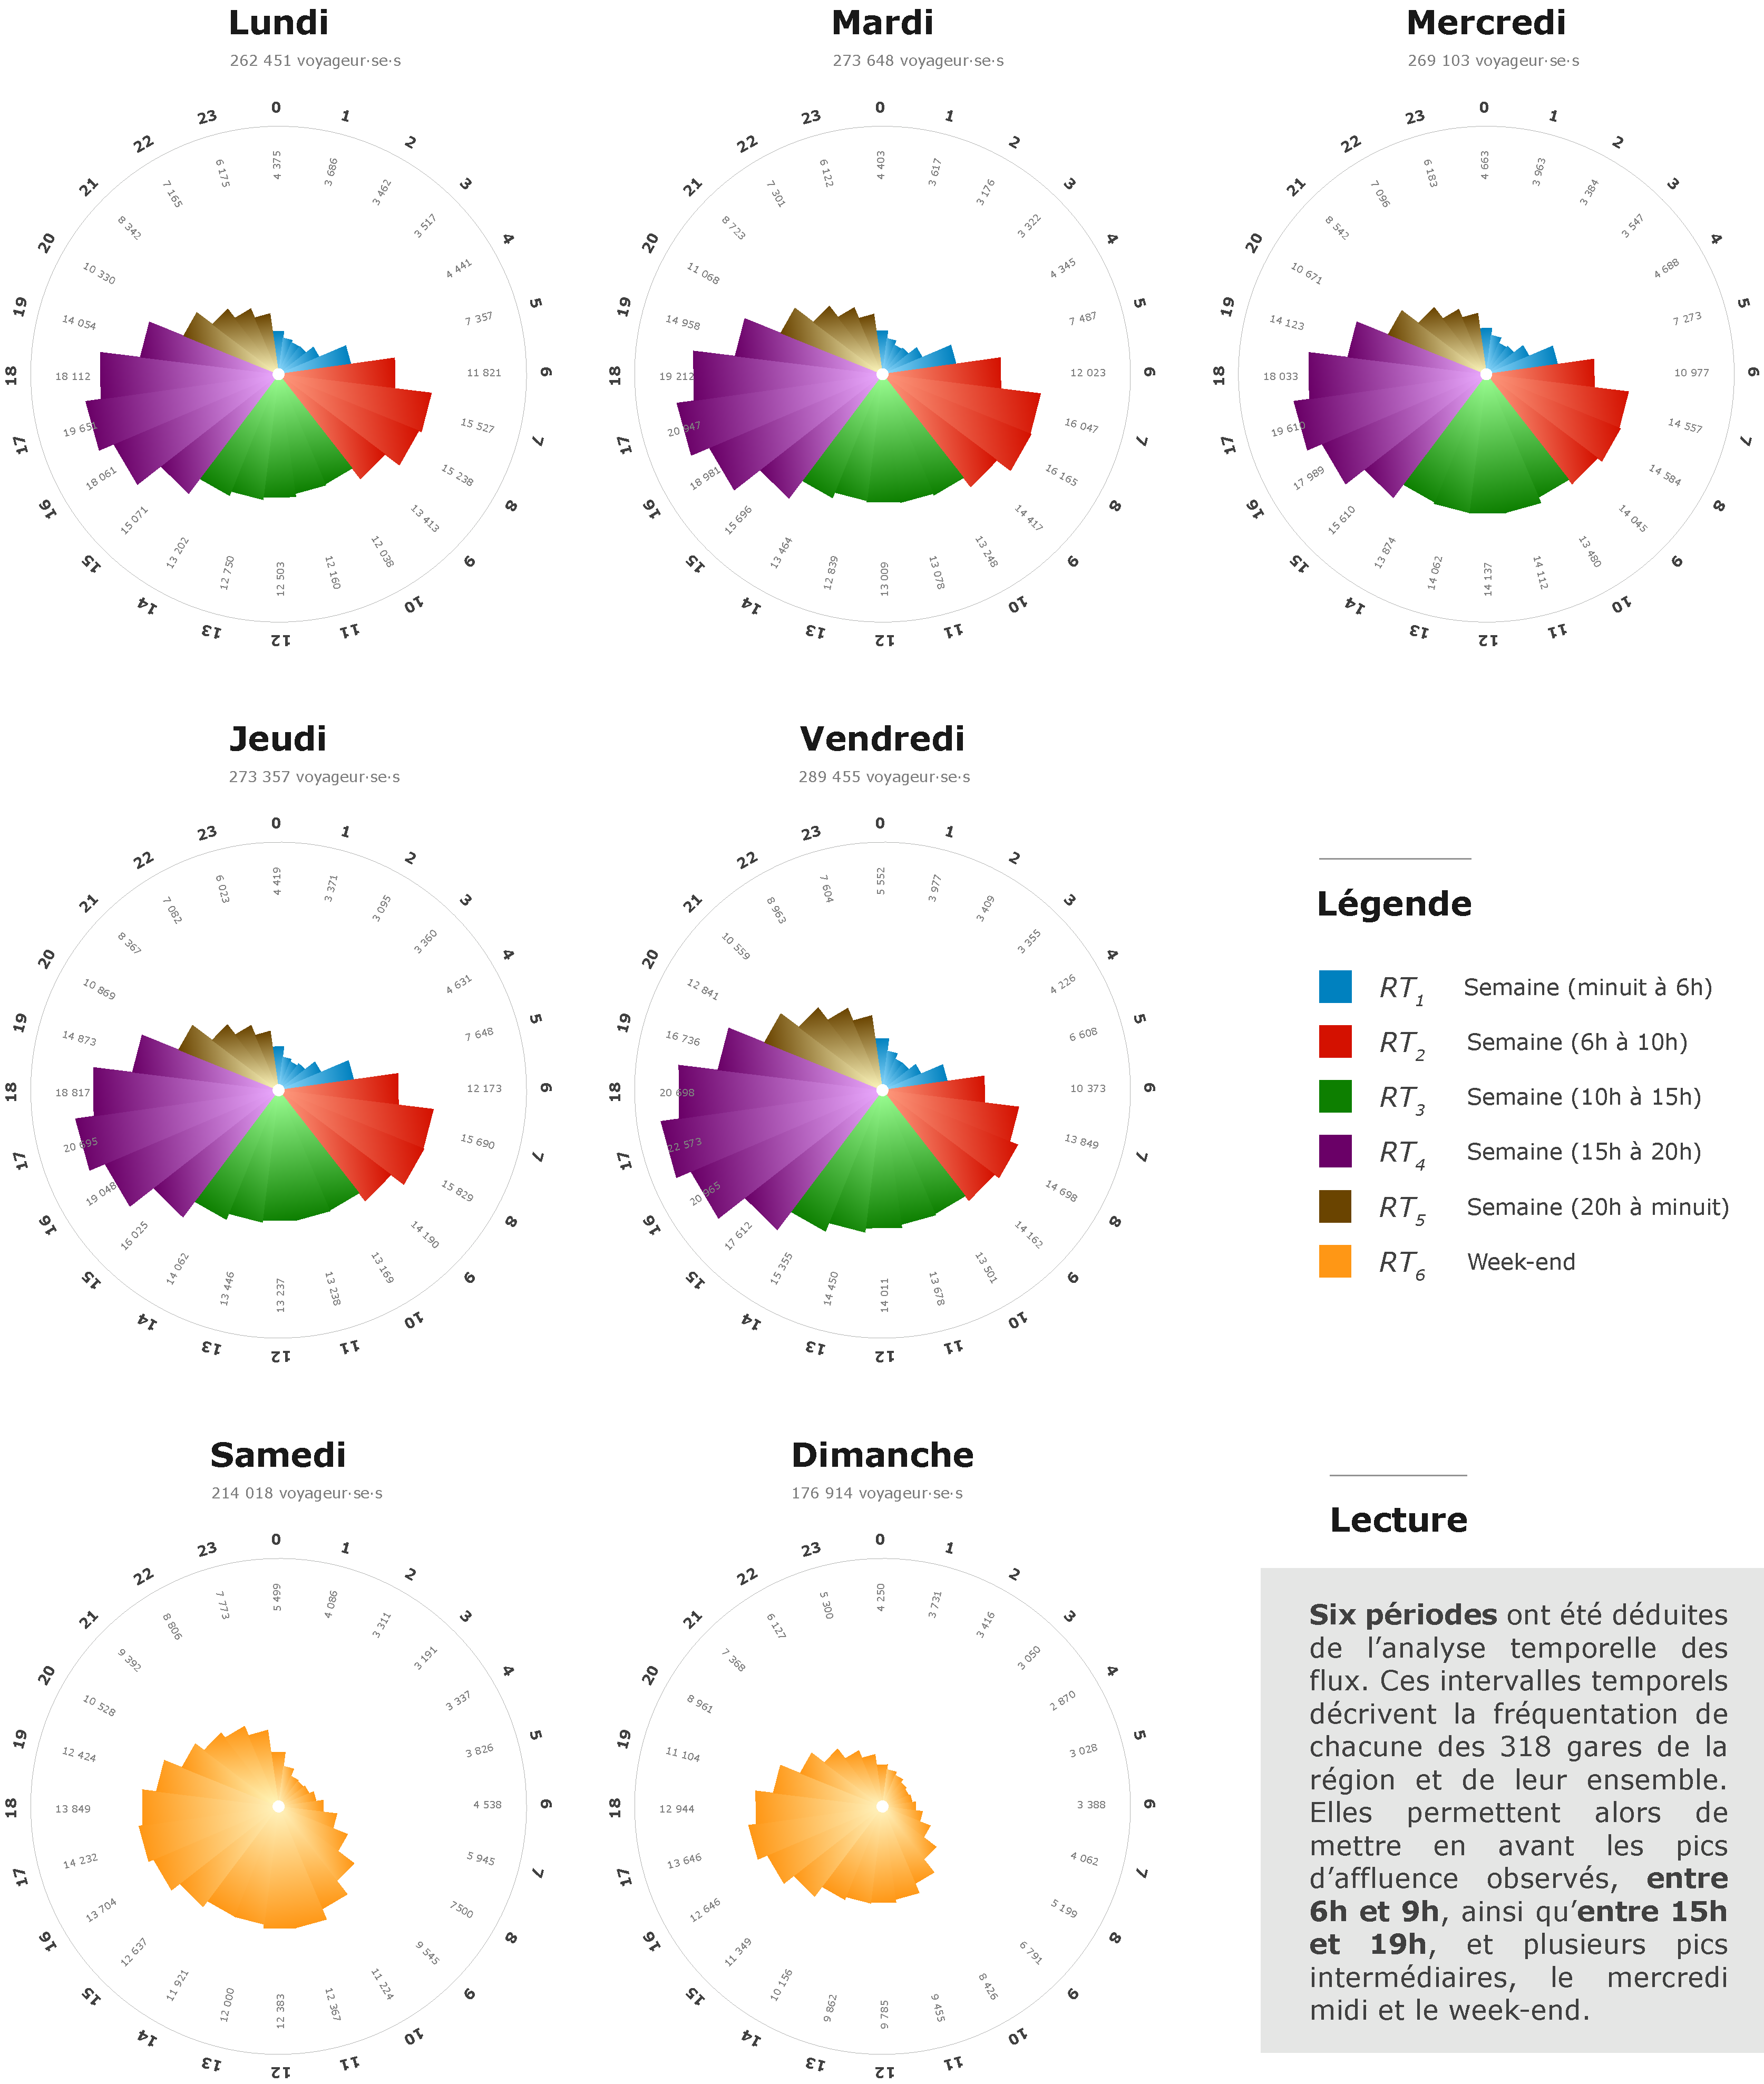
\includegraphics[width=1\columnwidth]{src/Figures/Chap-6/FR_NPART_Flux_frequentation.pdf}}
        \vspace{5pt}
        \begin{flushright}\scriptsize{
        Jeux de données~: \textcolor{blue}{\textcite{google_maps_google_2024}}\index{Google Maps@\textsl{Google Maps}|pagebf}
        \\
        Réalisation~: \textcolor{blue}{Dylan Moinse (2024)}
        \\
        Auteur·rice·s~: projet de recherche \acrshort{NPART}
        }\end{flushright}
    \end{figure}

    % Pics secondaires
Le mercredi se distingue également par un pic intermédiaire entre 10h et 12h, probablement dû à l'après-midi traditionnellement accordé aux enfants, alors que le vendredi enregistre un maximum de fréquentation plus prononcé durant la période de pointe du soir. L'identification d'un pic intermédiaire dans nos observations est étayée par les analyses de la distribution des déplacements effectuées par \textcolor{blue}{Emmanuel} \textcolor{blue}{\textcite[66]{munch_periodes_2017}}\index{Munch, Emmanuel|pagebf} sur le réseau SNCF Transilien pour 126 gares en 2015. Ce dernier désigne ces pics par l'expression \Guillemets{flancs de pointe}, situés à la transition entre les heures de pointe et les heures creuses.

    % Périodes
%Cette distribution des flux de passager·ère par période est dès lors inégale~: la période \(RT_{4}\) enregistre une proportion nettement supérieure de fréquentation comparée aux autres, tandis que \(RT_{1}\) est bien plus faible en comparaison (voir l'\hyperref[fig-chap6:resultats-frequentation-periode]{illustration~\ref{fig-chap6:resultats-frequentation-periode}}, page~\pageref{fig-chap6:resultats-frequentation-periode}).%%Rédigé%%

    % Transition
Bien que la fréquentation des gares soit connue pour une semaine spécifique, cette information demeure à la fois limitée et statique. Face à ce défi, la prédiction permet de dépasser cette observation ponctuelle en anticipant l’évolution des usages et des contextes externes. L’intérêt d’effectuer une prédiction des flux en gare réside, d’un point de vue statistique, dans l'amélioration continue du modèle et, d’un point de vue aménagiste, dans l’optimisation de la prise de décision. Dans cette optique, nous allons détailler l'approche prédictive du volume de passager·ère·s adoptée dans le cadre du modèle \acrshort{NPART}.%%Rédigé%%

    % 6.2.4.2.
    \needspace{1\baselineskip} % Réserve de l'espace
\subsubsection*{Ajustement et prédiction de la fréquentation des gares étudiées
    \label{chap6:methodologie-indicateurs-frequentation-prediction}
    }

    % Introduction
La prédiction du volume de passager·ère·s vise principalement à anticiper les flux afin de mettre en évidence les leviers d’action susceptibles de favoriser un report modal vers les transports en commun, tout en renforçant leur gestion. Le développement de modèles prédictifs répond au besoin d’améliorer continuellement ces modèles et de mieux prévoir les fluctuations dues à des événements, aux variations saisonnières ou à des tendances à long terme. À cette fin, au travers d’une collaboration scientifique entre le \acrfull{LVMT} de l'Université Gustave Eiffel, la \acrfull{SUSE} et la \acrfull{SCU}, nous avons appliqué plusieurs techniques statistiques issues du \textsl{Machine Learning}\footnote{
    L’apprentissage automatique (\textsl{Machine Learning}) est une sous-discipline de l’\acrfull{IA} qui permet aux systèmes informatiques d’apprendre de manière autonome à partir de données d'entrée. Un tel modèle est capable d’identifier des schémas, des relations et de réaliser des prédictions ou de prendre des décisions à partir de données d’entraînement supervisées. Le \textsl{Machine Learning} trouve des applications diverses, allant de la prédiction à la classification, en passant par la reconnaissance vocale et d’image, ainsi que l’analyse de texte. 
} en adoptant un modèle d'apprentissage d'ensemble (\textsl{ensemble learning})\footnote{
    L’apprentissage d'ensemble consiste à combiner plusieurs modèles, appelés \Guillemets{apprenants (faibles)}, afin d’améliorer la précision par rapport à un modèle unique. Cette approche de \textsl{Machine Learning} permet d’améliorer les performances globales en réduisant l’erreur de généralisation, c’est-à-dire la différence entre les performances sur les données d’entraînement et celles sur de nouvelles données (i), la variance des modèles en lissant les prédictions individuelles (ii) et les biais du modèle (iii).
}, après avoir normalisé les données recueillies~:
\begin{customitemize}
    \item La \acrfull{MLR}, ou régression multiple linéaire, modélise la relation linéaire entre les variables explicatives et la variable cible, à savoir le nombre de voyageur·se·s ferroviaires~;
    \item La \acrfull{KNN}, ou la méthode des~k plus proches voisins, prédit la fréquentation en identifiant les \(k\) moments les plus similaires dans le passé et en calculant une moyenne des fréquentations correspondantes~;
    \item Les \acrfull{ANN}, ou réseaux de neurones, capturent les relations complexes et non linéaires entre les variables, en s'inspirant de l'architecture du cerveau humain.
    %\item Les \acrfull{SVM}, ou \textsl{Support Vector Machines}, et la régression logistique utilisés pour modéliser les relations entre les variables lorsque les techniques précédentes ne sont pas adaptées.
\end{customitemize}%%Rédigé%%

    % Ensemble learning
Les techniques d'apprentissage d'ensemble que nous avons employées sont la moyenne ensembliste\footnote{
    Dans cette approche, tous les modèles sont pondérés de manière égale, et la prédiction finale est calculée comme la moyenne des prédictions individuelles.
}, la moyenne pondérée ensembliste\footnote{
    Dans ce cas, les modèles sont pondérés en fonction de leurs performances respectives sur l'ensemble d'entraînement ; les modèles les plus précis se voient attribuer un poids plus élevé.
} et l'apprentissage par empilement\footnote{
    L'apprentissage par empilement, ou \textsl{stack learning}, consiste à utiliser les prédictions des modèles de base comme entrées pour un méta-modèle (dans notre cas, une régression de crête), qui produit la prédiction finale.
}. L'évaluation de ces modèles a été réalisée à l'aide des métriques basées sur l'\acrfull{MSE}\footnote{
    Comme décrit dans la \hyperref[section-chap4:cyclabilite-genre]{section examinant les liens entre la cyclabilité et l'usage genré de la mobilité individuelle légère~\ref{section-chap4:cyclabilite-genre}} (page~\pageref{section-chap4:cyclabilite-genre}), du \hyperref[chap4:titre]{chapitre~4~\ref{chap4:titre}} (page~\pageref{chap4:titre}), l'\acrfull{MSE} est une métrique couramment employée pour mesurer l'écart entre les valeurs observées et les valeurs prédites par un modèle de \textsl{Machine Learning}, en particulier dans les modèles de régression. Un des inconvénients de cette mesure est qu'elle amplifie les grandes erreurs en raison de l'élévation au carré des différences, rendant ainsi le modèle plus sensible aux valeurs aberrantes (\textsl{outliers}).
} et l'\acrfull{APRE}, ou l'erreur relative point par point moyenne\footnote{
    L'\acrfull{APRE} quantifie l'erreur relative entre les valeurs observées et les valeurs prédites, en la normalisant par rapport aux valeurs réelles. Cette \gls{métrique} est particulièrement utile pour évaluer la précision des modèles de prédiction lorsque les données présentent des variations importantes en amplitude. Contrairement à la \acrshort{MSE}, l'\acrshort{APRE} est moins sensible aux outliers puisqu'elle tient compte de l'échelle des valeurs réelles. 
}. Dans ces deux métriques, une valeur faible indique un modèle performant, capable de prédire les valeurs réelles avec précision tout en limitant les erreurs relatives.%%Rédigé%%

    % Figure Prédiction ridership
    \begin{figure}[h!]\vspace*{4pt}
        \caption{Méthodes de prédiction de la fréquentation en gare lors des heures de pointe matinales (\(RT_{2}\)).}
        \label{fig-chap6:prediction-frequentation}
        \centerline{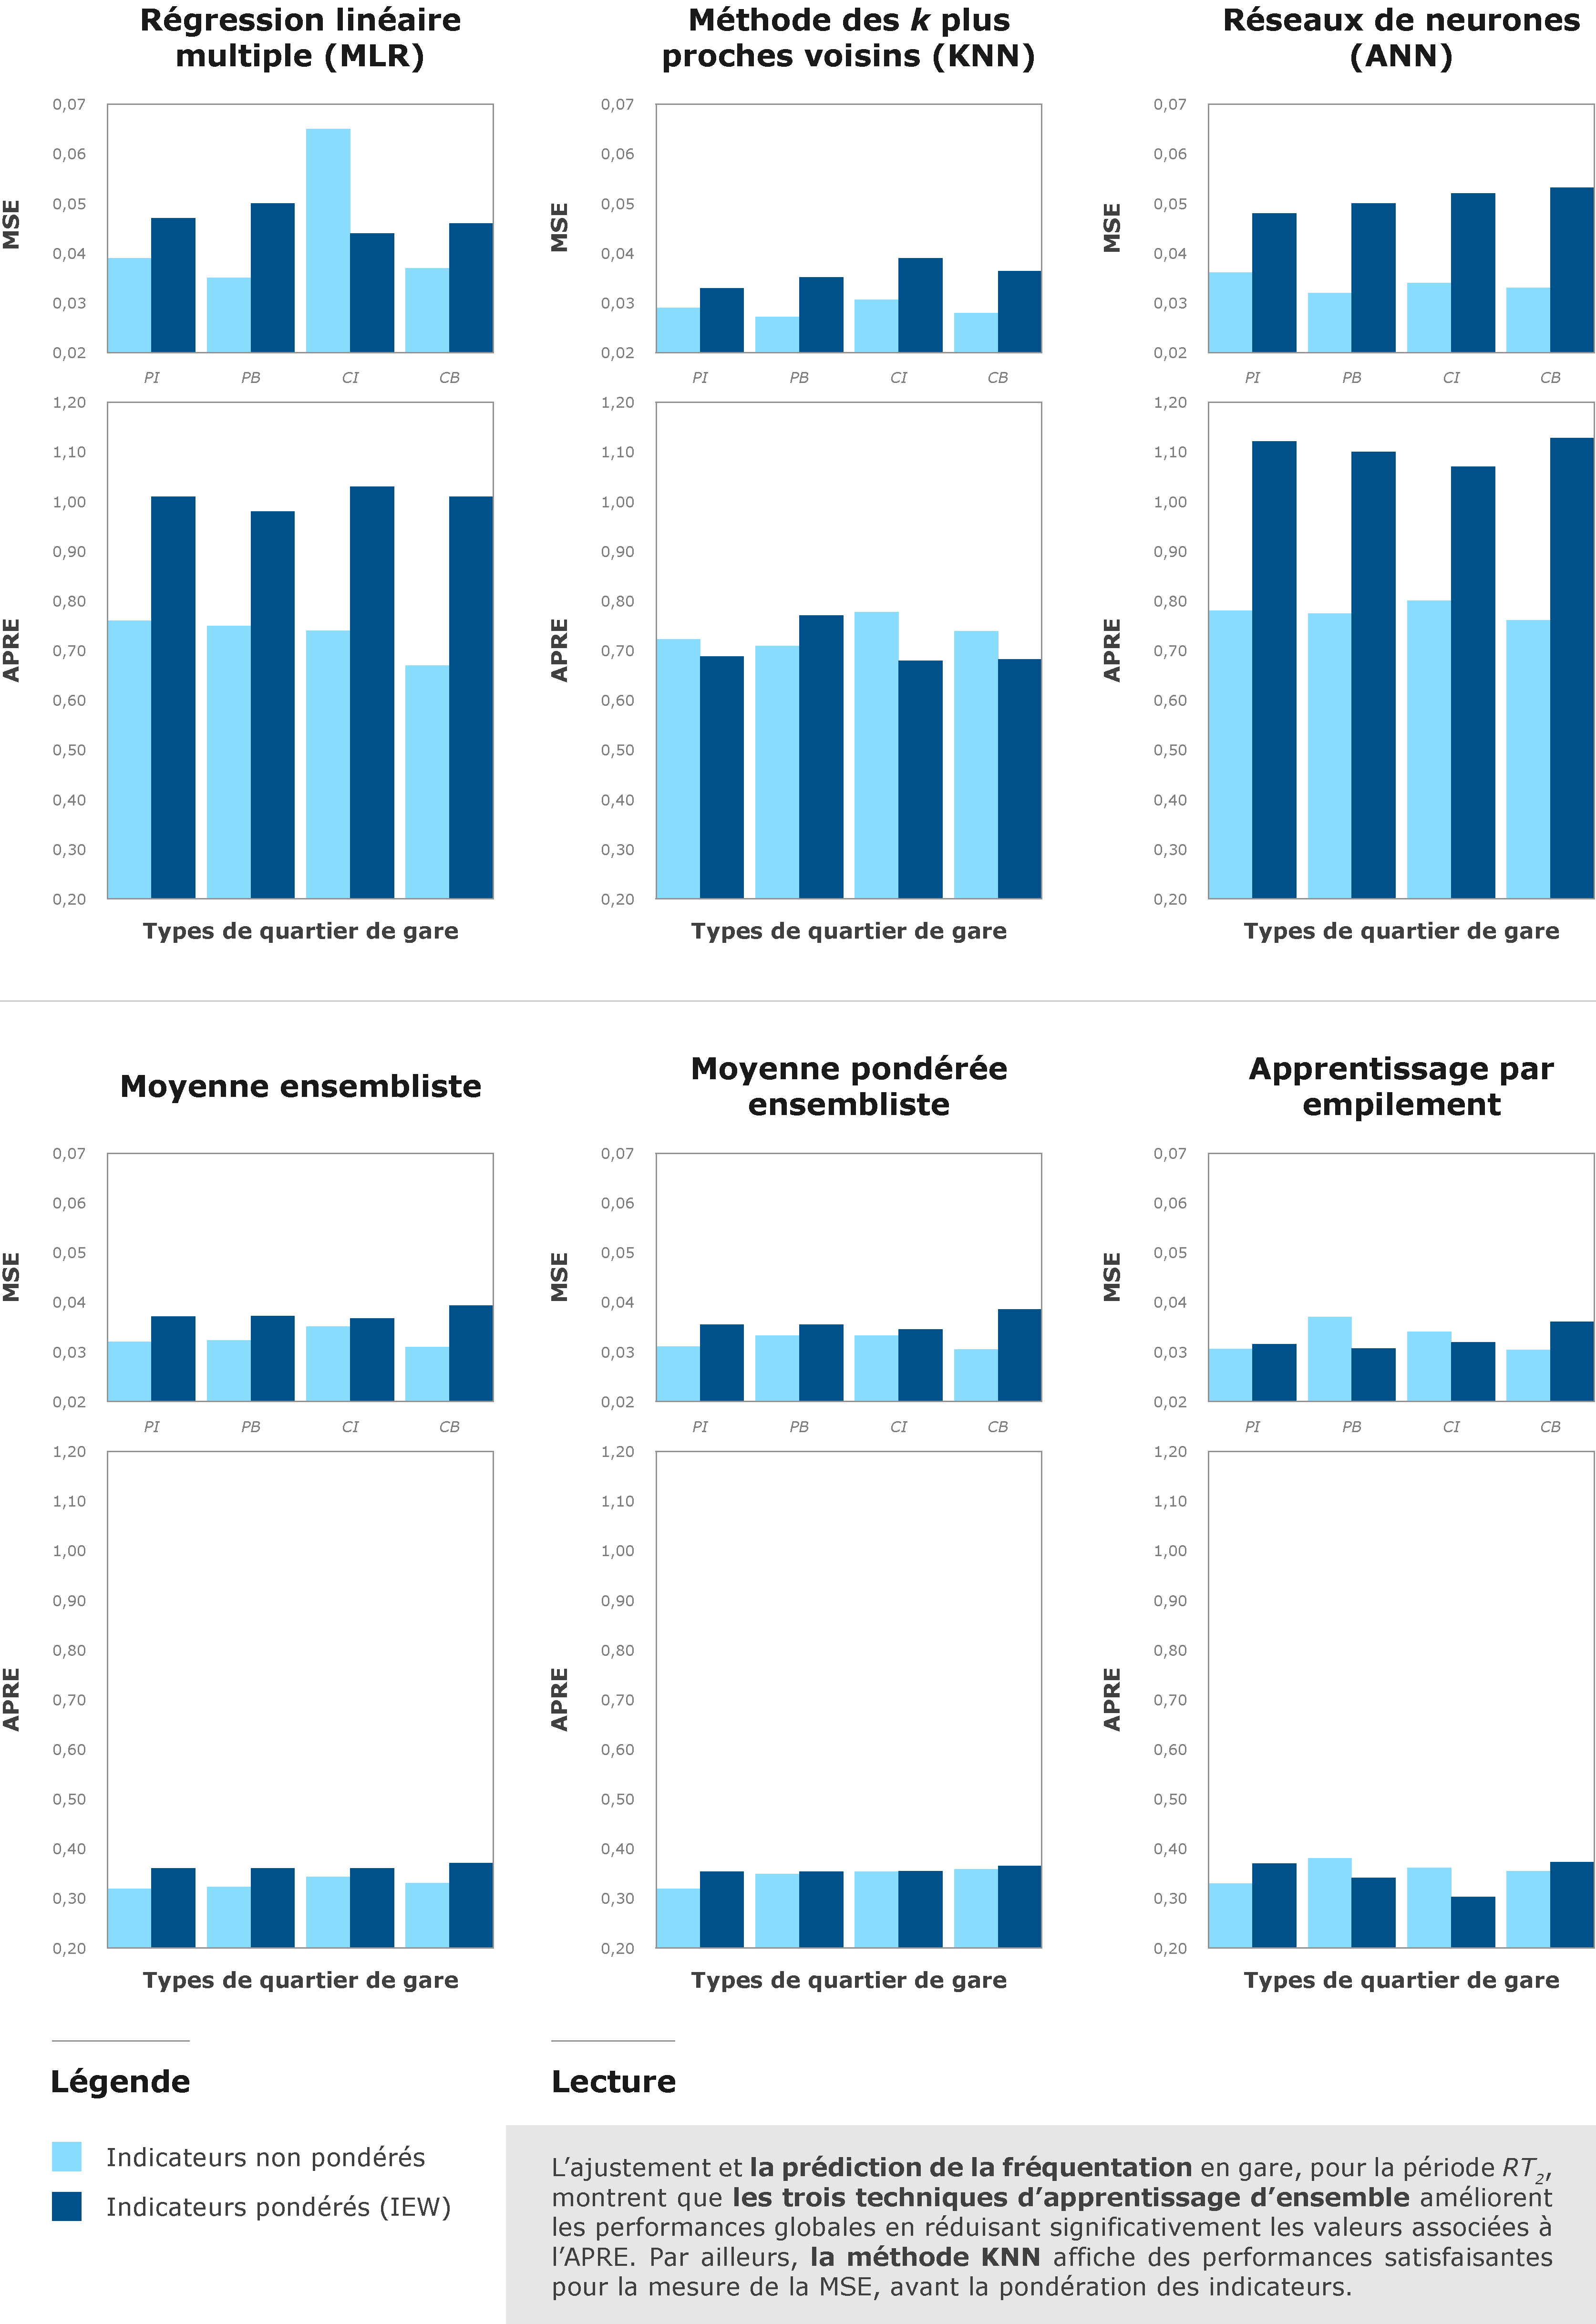
\includegraphics[width=1\columnwidth]{src/Figures/Chap-6/FR_NPART_Prediction_frequentation.pdf}}
        \vspace{5pt}
        \begin{flushright}\scriptsize{
        Réalisation~: \textcolor{blue}{Dylan Moinse (2024)}
        \\
        Auteur·rice·s~: projet de recherche \acrshort{NPART}
        }\end{flushright}
    \end{figure}

    % Résultats prédiction
Les résultats obtenus à partir de ces modèles prédictifs indiquent que les trois techniques d'apprentissage d'ensemble réduisent significativement l'\acrshort{APRE}, suggérant ainsi une amélioration des performances, en particulier pour les gares à faible affluence (voir l'\hyperref[fig-chap6:prediction-frequentation]{illustration~\ref{fig-chap6:prediction-frequentation}}, page~\pageref{fig-chap6:prediction-frequentation}). Bien que la méthode \acrshort{KNN} affiche des performances satisfaisantes avant la pondération des variables explicatives, les modèles \acrshort{MLR} et \acrshort{ANN} montrent des améliorations notables après l'application de cette pondération. Nous avons comparé l'évolution des valeurs de la \acrshort{MSE} et de l'\acrshort{APRE} en fonction des différents périmètres géographiques et des périodes. Cette analyse a permis de démontrer que le \acrshort{KNN} ainsi que les trois modèles prédictifs basés sur l'apprentissage d'ensemble offrent un ajustement plus précis dans la prédiction de la fréquentation des gares. Il en ressort que ces modèles prédictifs bénéficient particulièrement aux gares moins fréquentées, pour lesquelles la précision des prévisions s'avère améliorée.%%Rédigé%%

    % Transition questionnaire opinion et poids relatif des indicateurs
Une fois la grille d'indicateurs définie et l'extraction des données géographiques réalisée, se pose la question de leur pondération relative dans le cadre de la classification des gares et des quartiers de gare. Alors que la grande majorité des modèles \acrshort{NPM} précédents attribue un poids égal à chaque indicateur, une poignée de recherches souligne les limites de cette méthode de calibration, susceptibles d'altérer la validité du processus de classification. Dans ce contexte, la section suivante est consacrée à l'exposé des différentes stratégies de pondération que nous avons élaborées pour notre modélisation.%%Rédigé%%

    % Transition
Après avoir défini le \acrshort{NPART} en nous appuyant sur une grille d’indicateurs organisée autour de quatre dimensions clés~–~le nœud, le lieu, l'accessibilité et la fréquentation~–, nous nous attachons à décrire les étapes de calibration du modèle. L'objectif de la section suivante est alors d'ajuster et de valider les paramètres de l'outil mobilisé. À cette fin, nous allons explorer les méthodes de collecte et d'analyse des données géographiques, et la manière dont ces techniques permettent d'assurer une meilleure précision dans les résultats tirés de ce modèle couplant réseau et urbanisme.%%Rédigé%%

     % ___________________________________________
    % 6.3.
    \newpage
    \needspace{1\baselineskip} % Réserve de l'espace
    \sectionheader{Méthodes de collecte et d'analyse des données géographiques}
\section{Protocole de collecte et d'analyse des données en vue de modéliser le degré de coordination entre le réseau et l'urbanisme, à l’échelle de la région Hauts-de-France
    \label{chap6:methodologie-m-tod-index}
    }

    % Introduction
La conception de notre modèle \acrshort{NPART} repose sur la sélection de quarante indicateurs explicatifs quantifiables et de six indicateurs relatifs à la fréquentation des gares. L’objectif étant de classifier et de qualifier les gares ainsi que leur environnement immédiat, dans le cadre du développement d’un \acrshort{M-TOD}, un protocole méthodologique a été mis en place. Celui-ci inclut la collecte des données ainsi que leur analyse géostatistique. La méthodologie détaillée dans cette section présente les techniques employées pour l’extraction, la normalisation et la validation des mesures. Ce projet de recherche s'inscrit dans le cadre d'une collaboration scientifique internationale impliquant des chercheur·se·s de l'Université Gustave Eiffel, de \acrfull{SUSE} et de \acrfull{SCU}, les chercheur·se·s de ces deux universités chinoises ayant développé l'approche méthodologique présentée ici, au travers d’une collaboration et d’un dialogue interdisciplinaire avec les chercheur·se·s du \acrfull{LVMT}. Ce processus méthodologique intègre également la classification des gares selon différents critères ainsi que l’attribution de poids aux indicateurs, afin de mieux refléter leur influence relative sur l'usage du rail. Ce protocole d'analyse a conduit à la génération de 288 typologies spécifiques, en fonction de plusieurs facteurs~: la zone géographique analysée (\(PI\), \(PB\), \(CI\) et \(CB\)), les périodes étudiées (de \(RT_{1}\) à \(RT_{6}\)), les stratégies de pondération des variables et les procédés de classification appliqués aux gares (voir le \hyperref[fig-chap6:schema-methodologie]{schéma~\ref{fig-chap6:schema-methodologie}}, page~\pageref{fig-chap6:schema-methodologie}).%%Rédigé%%

    % Figure schéma méthodologie NPART
    \begin{figure}[h!]\vspace*{4pt}
        \caption{Diagramme de flux représentant les principales étapes méthodologiques du modèle spatial.}
        \label{fig-chap6:schema-methodologie}
        \centerline{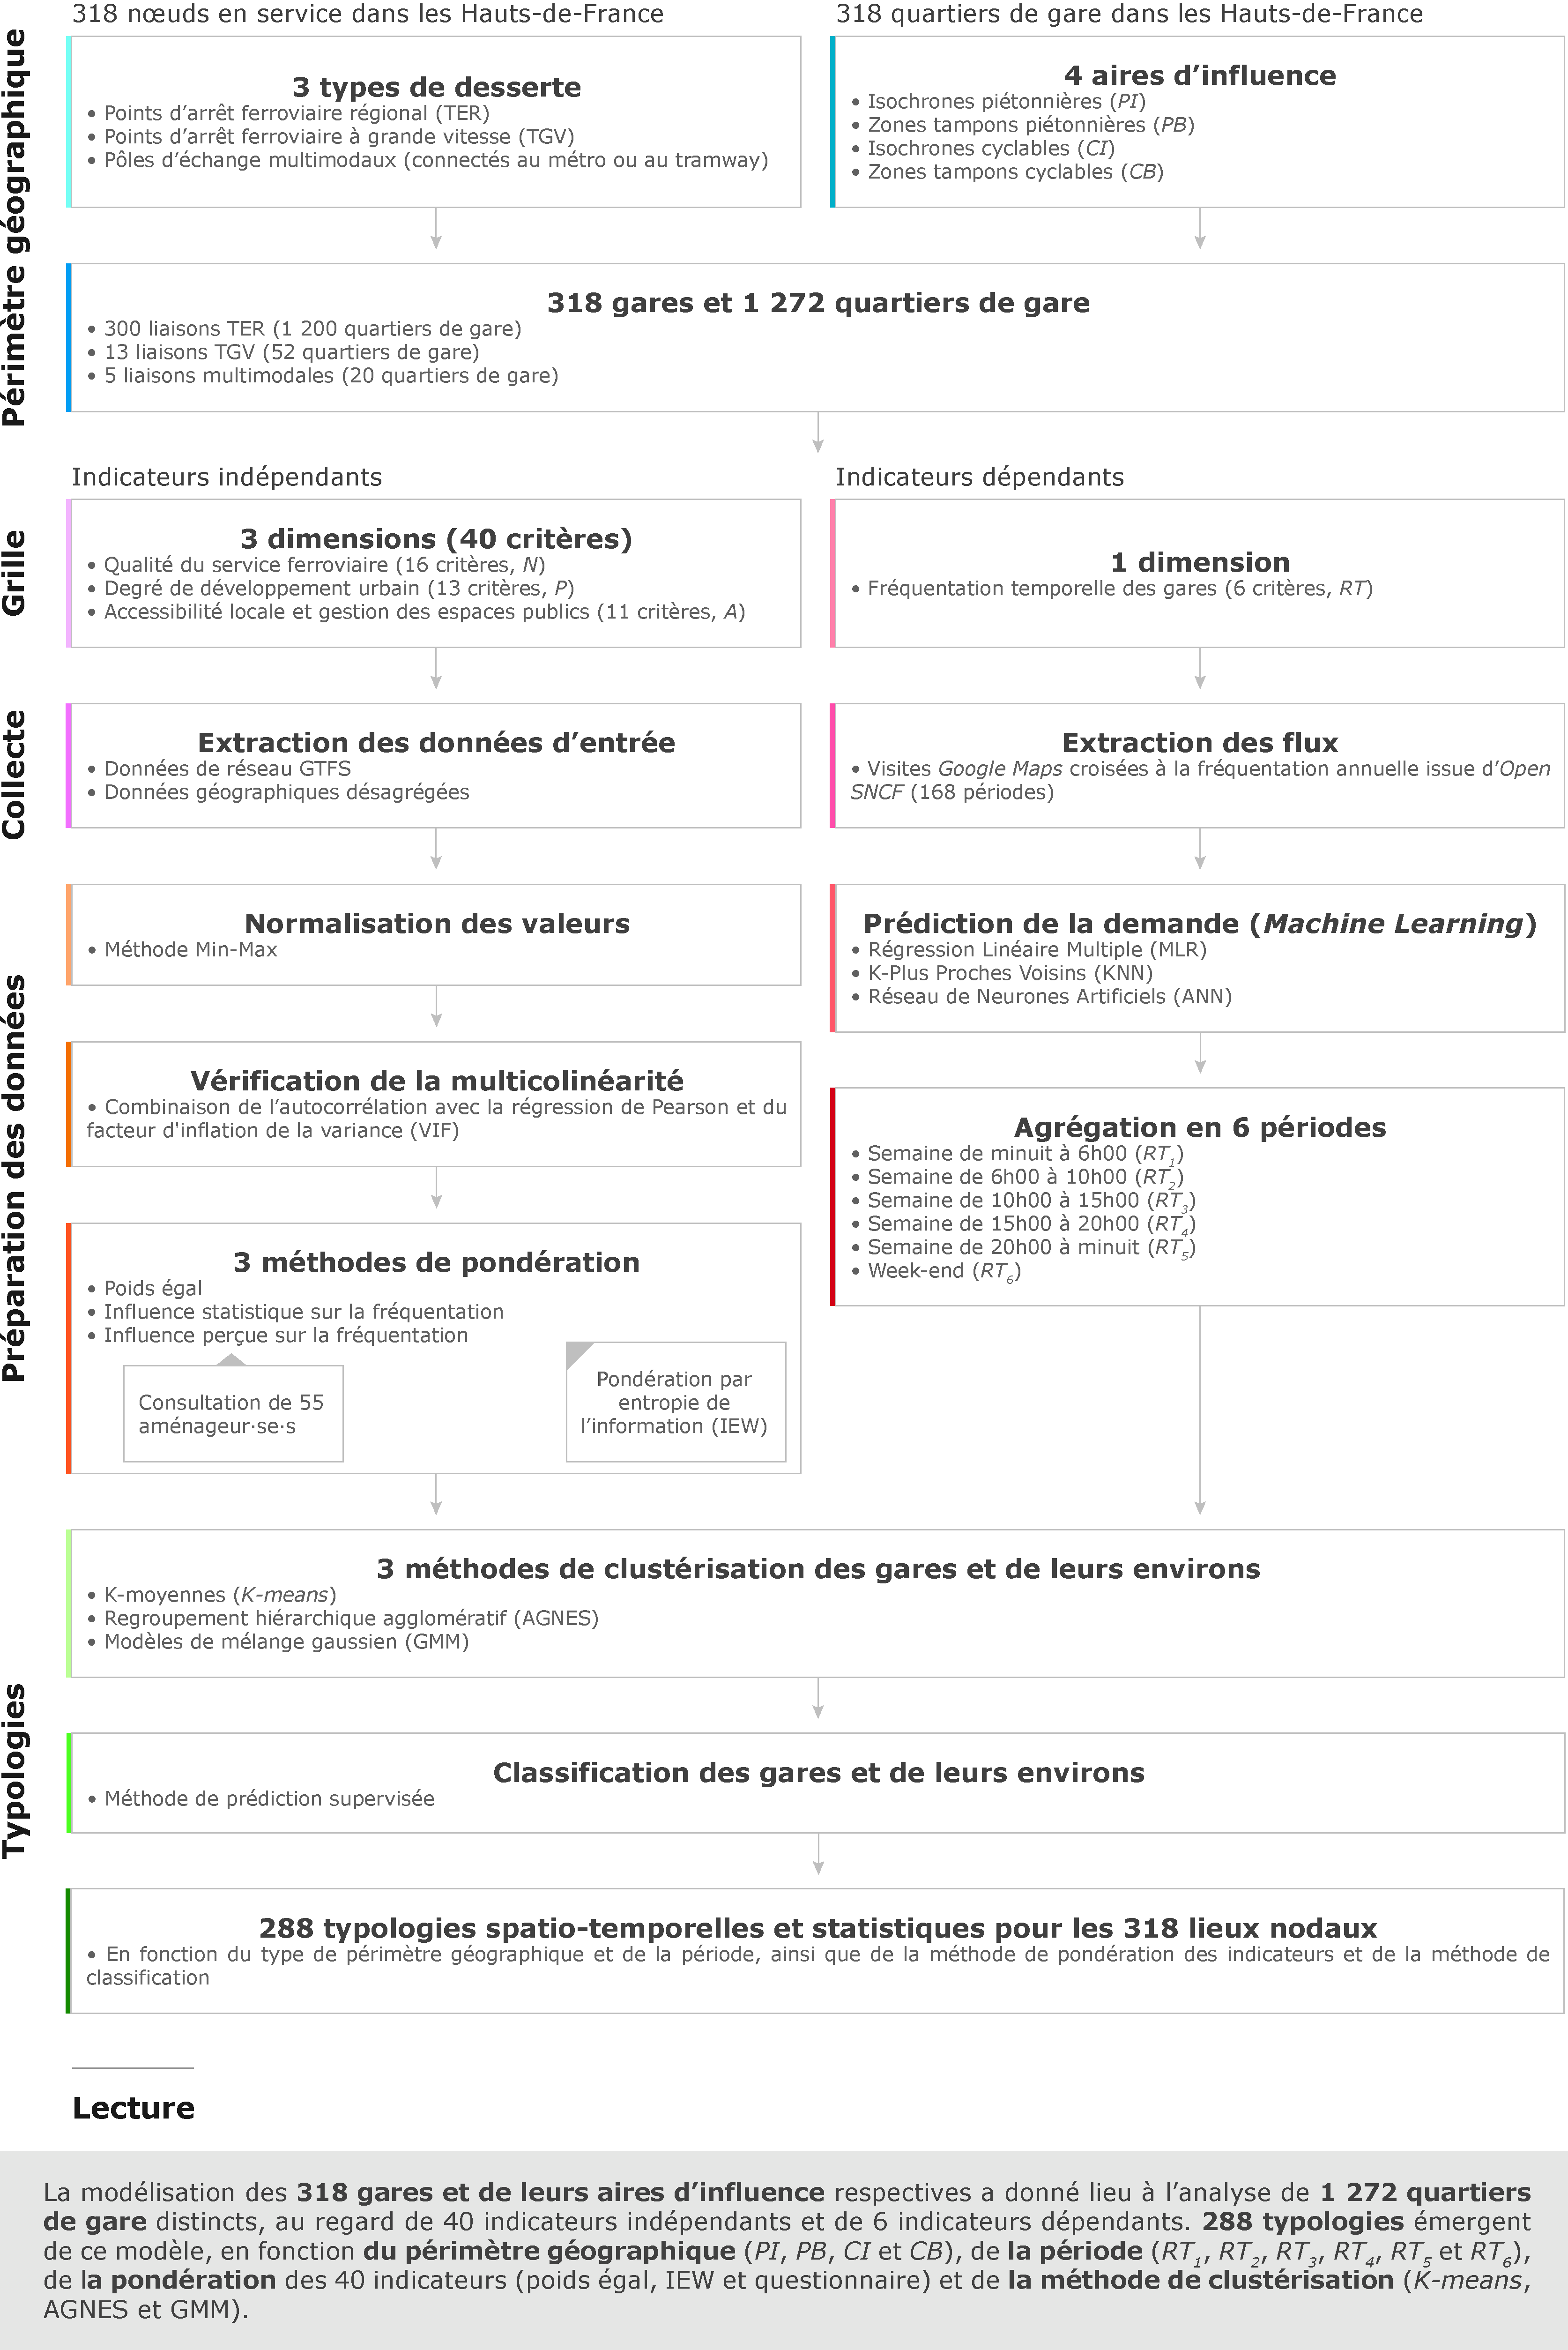
\includegraphics[width=1\columnwidth]{src/Figures/Chap-6/FR_NPART_Schema_Methodologie.pdf}}
        \vspace{5pt}
        \begin{flushright}\scriptsize{
        Réalisation~: \textcolor{blue}{Dylan Moinse (2024)}
        \\
        Auteur·rice·s~: projet de recherche \acrshort{NPART}
        }\end{flushright}
    \end{figure}

    % Annonce du plan
Quant à l'énoncé du plan, nous allons tout d’abord présenter les techniques de modélisation employées pour traiter les données recueillies, à savoir l’extraction et la normalisation des données statistiques et géographiques, leur validation à travers l’analyse des interactions qu’elles entretiennent entre elles ainsi que la manière dont les stations sont classifiées (voir la \hyperref[chap6:methodologie-statistiques]{section sur les processus d'extraction, d'exploitation et de classification}, page~\pageref{chap6:methodologie-statistiques}). Après quoi, le sujet portera sur l’attribution des poids aux variables, en considérant trois approches~: un poids égal, une pondération statistique, fondée sur leur influence effective sur la fréquentation des gares et une pondération perçue, établie à partir des retours des aménageur·se·s interrogé·e·s (voir la \hyperref[chap6:methodologie-ponderation-indicateurs]{section sur le poids relatif de chaque volet}, page~\pageref{chap6:methodologie-ponderation-indicateurs}). Enfin, sera évoquée la validité, la mise à jour et la valorisation de ce modèle à travers sa reproductibilité et son automatisation (voir la \hyperref[chap6:conclusion-valorisation]{section sur les exigences d'un modèle transparent capable d'être répliqué et répété}, page~\pageref{chap6:conclusion-valorisation}).%%Rédigé%%

    % 6.3.1.
    \needspace{1\baselineskip} % Réserve de l'espace
\subsection{Techniques de modélisation des données recueillies
    \label{chap6:methodologie-statistiques}
    }

    % Introduction
Cette sous-section décrit les étapes de collecte et d'analyse des données statistiques liées aux gares ainsi qu'aux informations géographiques, en lien avec les zones tampons et les isochrones définies. La préparation des données qui précède le travail de modélisation s’appuie principalement sur la recherche de sources de données désagrégées, lesquelles sont ensuite transformées et mises à l’échelle pour garantir leur cohérence. Par ailleurs, la validation du modèle s'établit sur l’analyse des interdépendances entre les différents indicateurs. À la suite de cette exploitation statistique, nous pouvons adopter une approche par classification, basée sur divers paramètres exposés.%%Rédigé%%

    % 6.3.1.1.
    \needspace{1\baselineskip} % Réserve de l'espace
\subsubsection*{Extraction et normalisation des données géographiques
    \label{chap6:methodologie-statistiques-normalisation}
    }

    % Extraction géographique - quartiers de gare
Une fois la grille d'indicateurs définie de manière détaillée, nous avons procédé à l'extraction spatiale des données disponibles. Pour chaque point d'échange, nous avons retenu les quartiers de gare définis, en intégrant à la fois les isochrones et les zones tampons piétonnes (\(PB\) et \(PI\)) et cyclables (\(CB\) et \(CI\)), telles que formulées dans la \hyperref[chap3:quartiers-gare-analyse-geostatistique]{section consacrée à la représentation géographique des quartiers de gare de la région} (page~\pageref{chap3:quartiers-gare-analyse-geostatistique}), dans le \hyperref[chap3:titre]{chapitre~3} (page~\pageref{chap3:titre}). Nous nous sommes délibérément restreints à l'exploitation de données géographiques désagrégées afin de maximiser la précision de la localisation des variables déterminées, à l'exception des valeurs relatives au nœud, qui reposent exclusivement sur les données \acrshort{GTFS} fournies par les institutions et les gestionnaires de mobilité. Qui plus est, cet impératif du point de vue de la granularité spatiale s'est traduite par l'adoption de méthodes d'estimation des données lorsque celles-ci sont regroupées au sein de grilles spatiales, telles que les données carroyées ou les hexagones, comme détaillé dans la \hyperref[chap3:quartiers-gare-analyse-geostatistique]{section consacrée à la représentation géographique des quartiers de gare de la région} (page~\pageref{chap3:quartiers-gare-analyse-geostatistique}), dans le \hyperref[chap3:titre]{chapitre~3} (page~\pageref{chap3:titre}).%%Rédigé%%

    % Python VS SIG
À cet égard, nous avons opté pour l'utilisation exclusive du langage de programmation \textsl{Python}, en particulier ses différentes bibliothèques dédiées à la géospatialisation\footnote{
    \textsl{Python} dispose d'un vaste écosystème de bibliothèques pour la manipulation et la visualisation des données spatiales, dont les principales sont~: \textsl{GeoPandas}, \textsl{Shapely}, \textsl{Pyproj}, \textsl{Fiona}, \textsl{Rtree}, \textsl{GDAL}, \textsl{PySAL}, \textsl{Geopy}, \textsl{OSMNx}, \textsl{NetworkX}, \textsl{H3-Py}, \textsl{Folium}, \textsl{Basemap}, \textsl{Plotly}, \textsl{Geoplot}.
}, afin d'extraire et d'analyser les données. Ce choix s'explique par plusieurs avantages comparatifs par rapport à l'usage classique du \acrfull{SIG}. Tout d'abord, \textsl{Python} offre une flexibilité accrue dans le traitement des données, étant à la fois plus adaptable et facilement personnalisable. Ensuite, il permet la manipulation de jeux de données volumineux et l'automatisation des processus d'extraction et de transformation des données grâce aux différents scripts générés. Par ailleurs, \textsl{Python} facilite la réalisation de calculs complexes et permet ainsi l'obtention des données requises, notamment lorsque celles-ci nécessitent des combinaisons de jeux de données divers. Enfin, l'analyse des données \acrshort{GTFS} est grandement simplifiée, notamment en permettant la modélisation de réseaux complexes et l'analyse de graphes.%%Rédigé%%

    % Normalisation des données recueillies
La normalisation des données d'entrée est une étape critique avant toute modélisation, \textsl{a fortiori} dans le cadre du \acrshort{NPM}. Dans ce contexte, les données collectées pour chaque gare doivent être homogénéisées pour éviter que les différences d'échelle entre les variables n'influencent de manière disproportionnée les résultats du modèle. Pour cela, la méthode de normalisation Min-Max\footnote{
    Étant donné que les caractéristiques nodales comme celles de lieu, d'accessibilité ou de fréquentation peuvent être exprimées dans des unités distinctes, la normalisation permet d'uniformiser ces valeurs afin qu'elles puissent être intégrées de manière cohérente dans le \acrshort{NPART}, sans qu'un indicateur ou une dimension ne prenne le pas sur l'autre. Dans cette optique, la méthode Min-Max préserve la distribution relative des données tout en maintenant les relations entre les valeurs. Cette standardisation des variables assure l'usage de techniques d'analyse sensibles à l'échelle des données, telles que les régressions ou les algorithmes basés sur la distance (k-means), qui seront appliqués ultérieurement.
} a été appliquée avant la phase d'entraînement. Cette technique consiste à transformer les valeurs de chaque variable pour qu'elles soient comprises entre 0 et 1 (voir la \hyperref[equation:normalisation]{formule~\ref{equation:normalisation}}, page~\pageref{equation:normalisation}).%%Rédigé%%

    % Équation normalisation
\begin{equation}
\label{equation:normalisation}
\begin{aligned}
x_i' = \frac{x_i - \min(x_i)}{\max(x_i) - \min(x_i)}
\end{aligned}
\end{equation}
\begin{align*}
    &\text{où~:}\\
    &x \text{ est la valeur d'origine~;}\\
    &x' \text{ est la valeur normalisée~;}\\
    \min(x) \text{ et } \max(x) & \text{ sont les valeurs minimale et maximale.}\\
\end{align*}%%Rédigé%%

    % Transition
Après la collecte et la normalisation des données,il est important de s'assurer que les variables ainsi transformées sont prêtes à être intégrées dans le modèle. Une démarche préparatoire clé avant la modélisation consiste à vérifier la multicolinéarité\footnote{
    La multicolinéarité est une situation statistique dans laquelle plusieurs variables explicatives d'un modèle sont fortement corrélées entre elles. En d'autres termes, les variables indépendantes présentent une redondance, ce qui peut poser des problèmes pour l'interprétation des résultats dans les modèles de régression, comme la régression linéaire multiple. Lorsque la multicolinéarité est présente, les coefficients des indicateurs indépendants peuvent devenir instables, réduisant la précision des prédictions et la signification statistique. Le facteur d'inflation de la variance (\(VIF\)), supérieur à 100, tout comme les coefficients de corrélations, proches de 1 ou de -1, indiquent généralement une forte multicolinéarité entre les variables.
} des données, c'est-à-dire l'existence de corrélations excessives entre certaines variables. La présence de multicolinéarité peut compromettre l'interprétation des résultats du modèle et nuire à sa précision, notamment dans les analyses basées sur les relations entre variables. Ainsi, avant d'aborder la phase de modélisation à proprement parler, une analyse de la multicolinéarité s'avère indispensable pour valider la cohérence des données et garantir leur relative indépendance.%%Rédigé%%

    % 6.3.1.2.
    \needspace{1\baselineskip} % Réserve de l'espace
\subsubsection*{Validation des données géographiques collectées par l'analyse de leurs interactions
    \label{chap6:methodologie-statistiques-validation}
    }

    % Multicolinéarité
Nous avons évalué la multicolinéarité entre les variables indépendantes à l'aide de deux approches statistiques~: le coefficient de corrélation simple, en utilisant le coefficient de corrélation de Pearson \(R^{2}\), et le facteur d'inflation de la variance (\(VIF\)). En combinant ces deux méthodes, nous pouvons identifier et supprimer les variables indépendantes présentant des problèmes de collinéarité très élevés. Les \hyperref[fig-chap6:correlations-indicateurs-independants-PI]{matrices d'autocorrélation~\ref{fig-chap6:correlations-indicateurs-independants-PI}} et \hyperref[fig-chap6:correlations-indicateurs-independants-CI]{\ref{fig-chap6:correlations-indicateurs-independants-CI}} (pages \pageref{fig-chap6:correlations-indicateurs-independants-PI} et \pageref{fig-chap6:correlations-indicateurs-independants-CI}) illustrent les interrelations entre les critères explicatifs.%%Rédigé%%

    % Figure régressions indicateurs indépendants PI
    \begin{figure}[h!]\vspace*{4pt}
        \caption{Matrice de corrélation du modèle spatial, à l'échelle des isochrones piétonnes.}
        \label{fig-chap6:correlations-indicateurs-independants-PI}
        \centerline{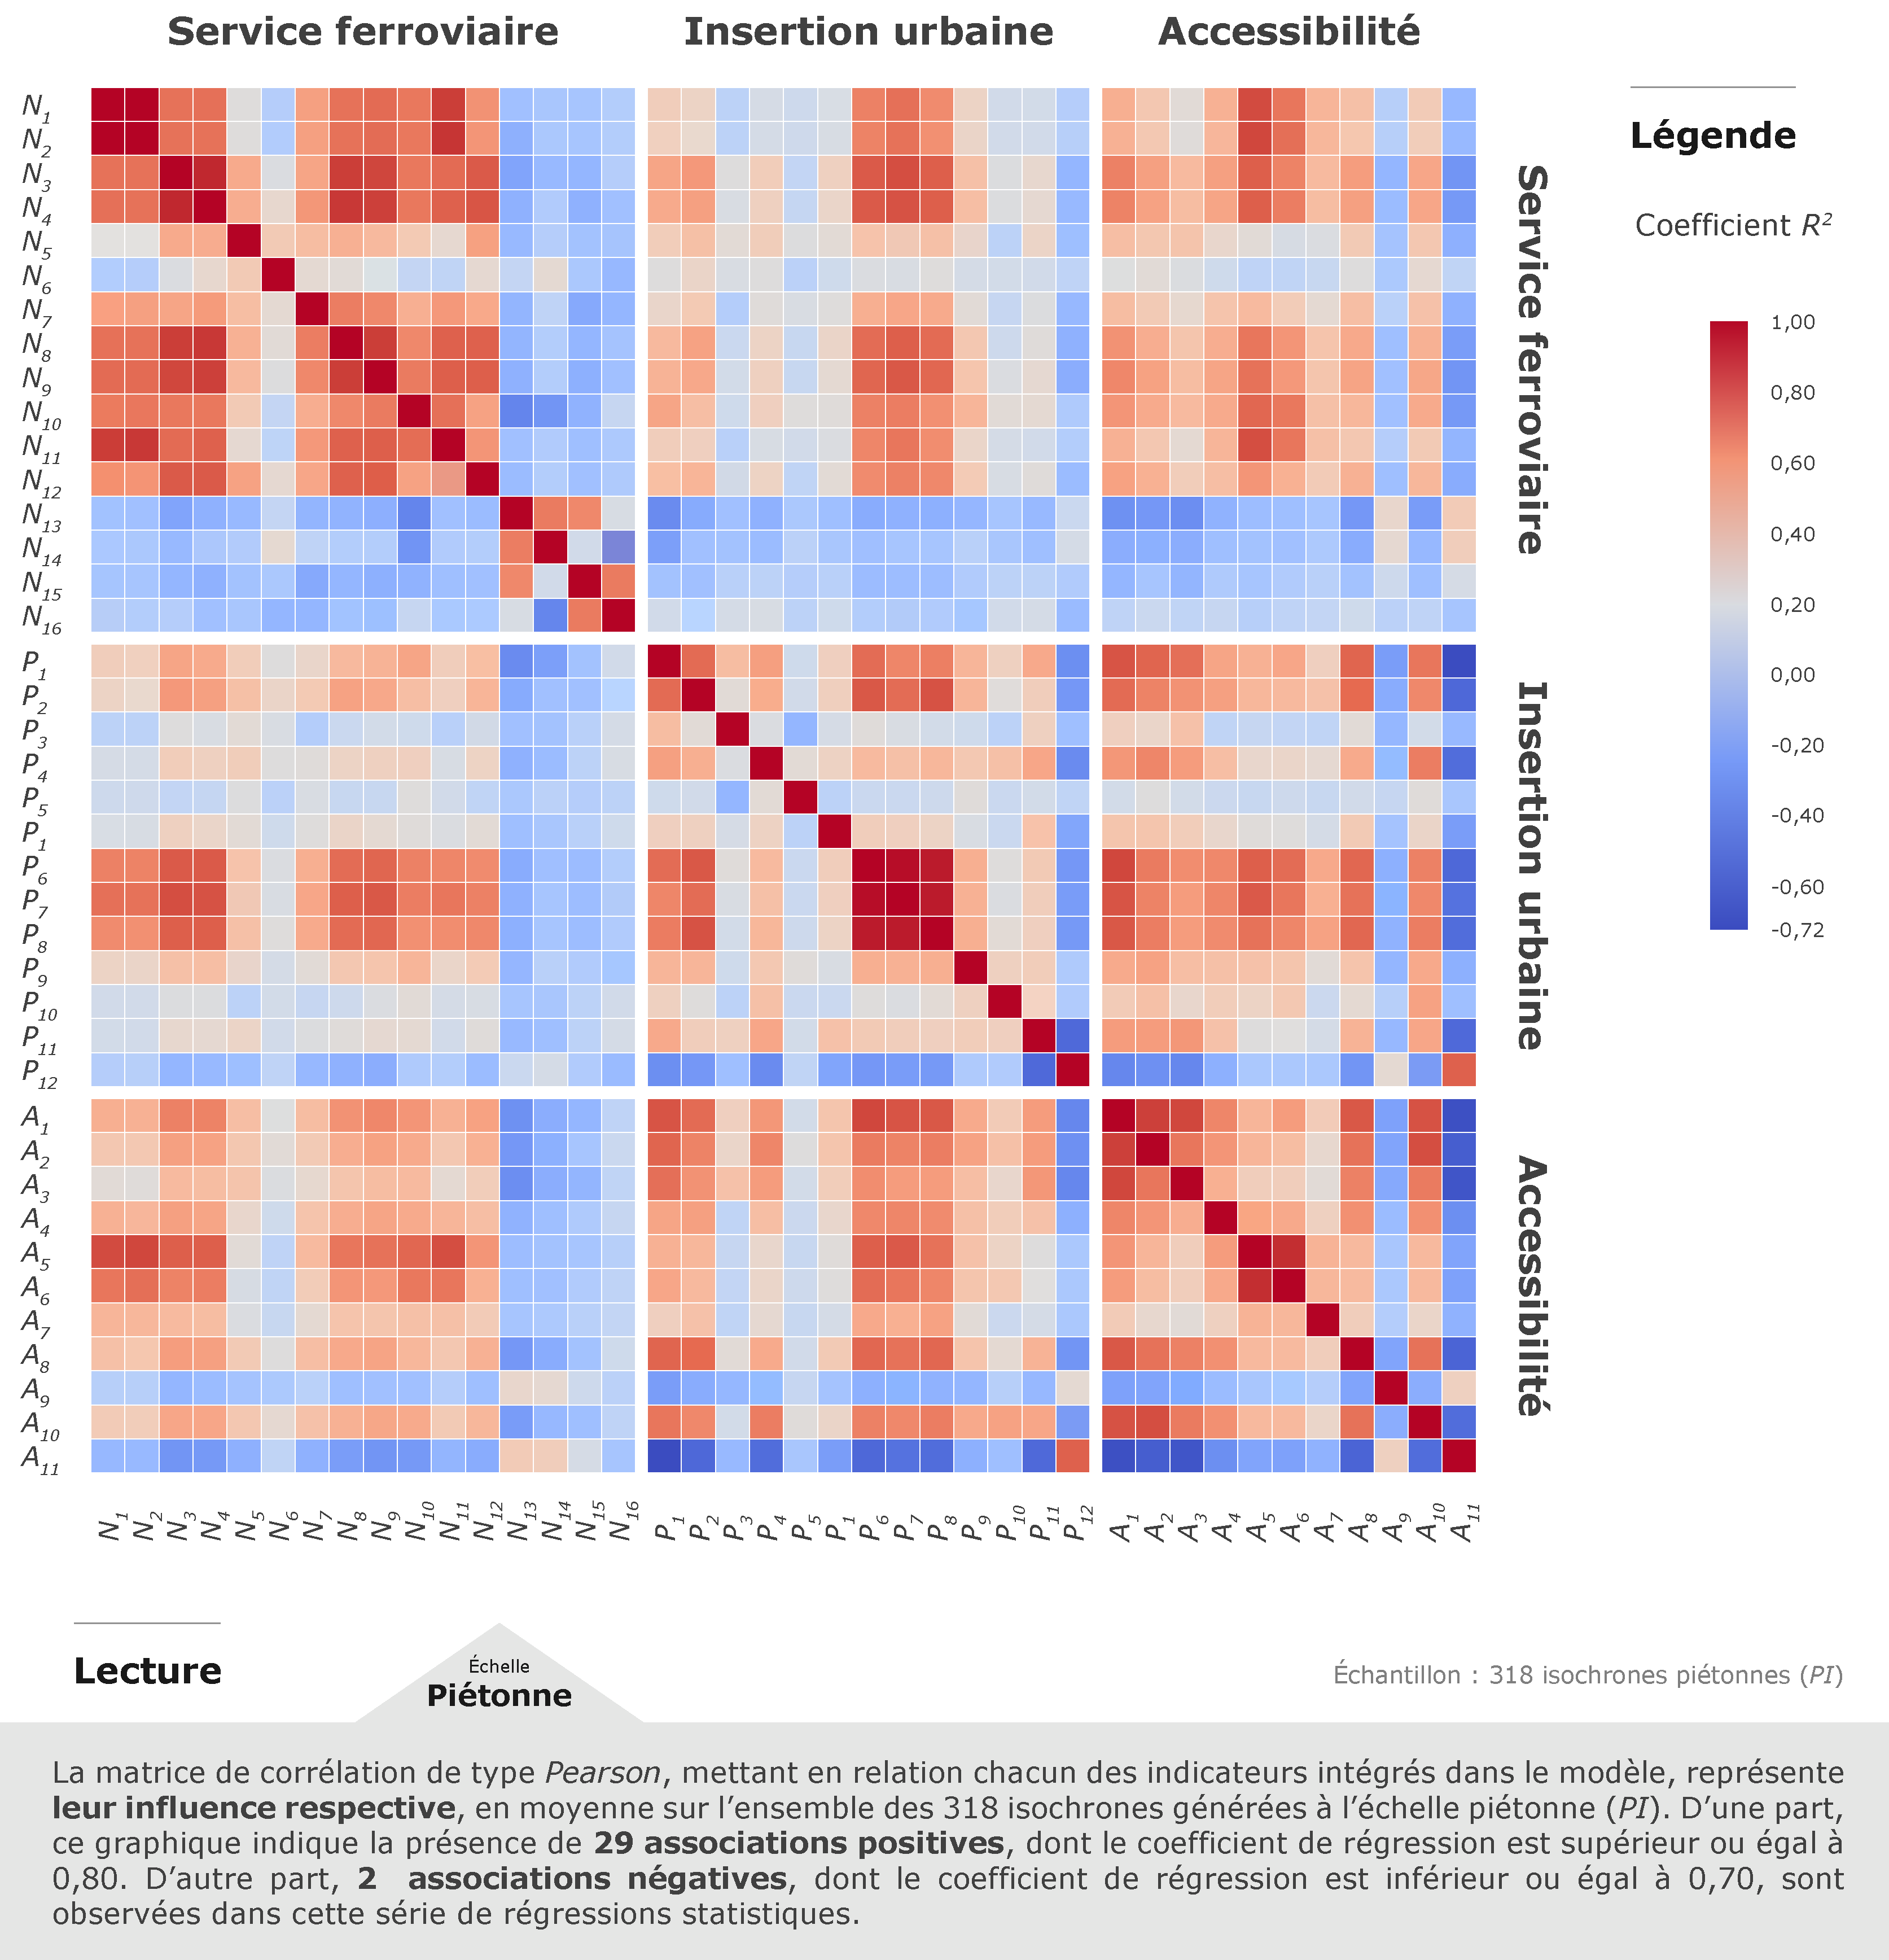
\includegraphics[width=1\columnwidth]{src/Figures/Chap-6/FR_NPART_Matrice_Correlation_PI.pdf}}
        \vspace{5pt}
        \begin{flushright}\scriptsize{
        Réalisation~: \textcolor{blue}{Dylan Moinse (2024)}
        \\
        Auteur·rice·s~: projet de recherche \acrshort{NPART}
        }\end{flushright}
    \end{figure}

    % Figure régressions indicateurs indépendants CI
    \begin{figure}[h!]\vspace*{4pt}
        \caption{Matrice de corrélation du modèle spatial, à l'échelle des isochrones cyclables.}
        \label{fig-chap6:correlations-indicateurs-independants-CI}
        \centerline{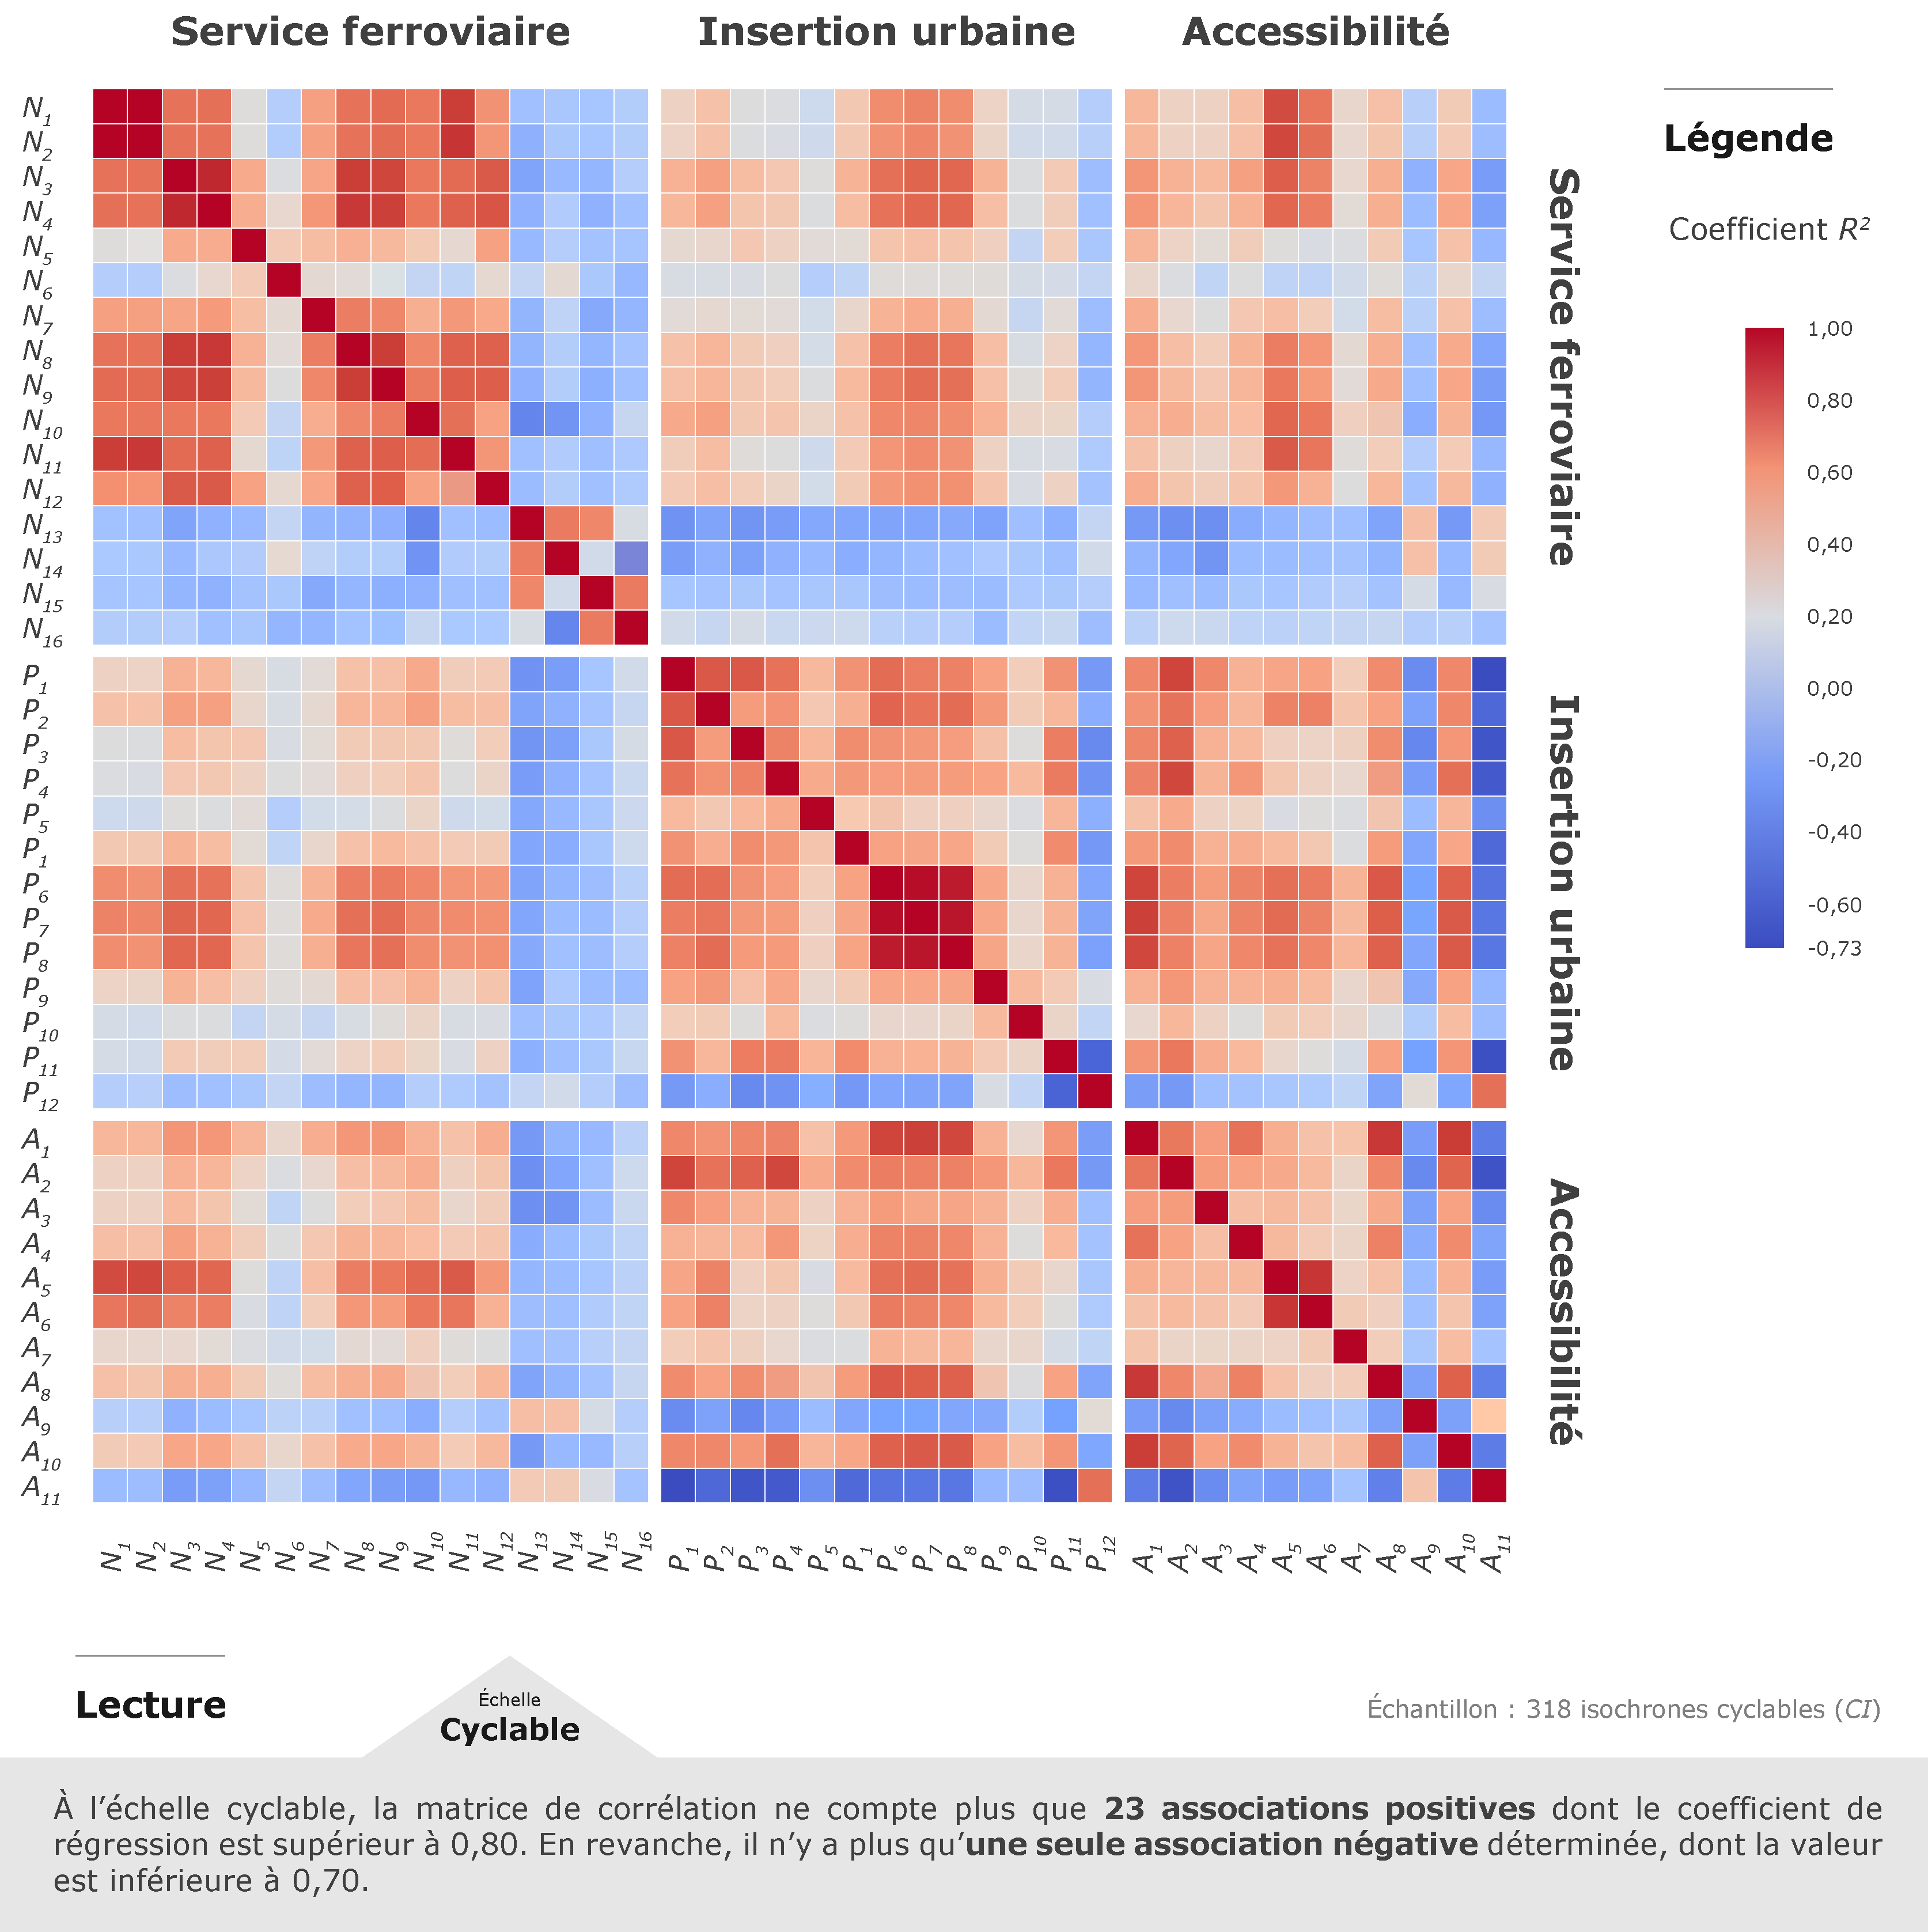
\includegraphics[width=1\columnwidth]{src/Figures/Chap-6/FR_NPART_Matrice_Correlation_CI.pdf}}
        \vspace{5pt}
        \begin{flushright}\scriptsize{
        Réalisation~: \textcolor{blue}{Dylan Moinse (2024)}
        \\
        Auteur·rice·s~: projet de recherche \acrshort{NPART}
        }\end{flushright}
    \end{figure}

    % Résultats corrélation : au sein de node
Au sein de la dimension liée au niveau de service en gare, la régression suggère que la fréquence du réseau \acrshort{TER} (\(N_{3}\) et \(N_{4}\)) présente une association positive significative, non seulement avec le nombre de directions desservies (\(N_{8}\), \(R^{2}\) à 0,89 et 0,90), mais aussi avec le degré de centralité (\(N_{9}\), \(R^{2}\) à 0,86 et 0,88) et avec le nombre de stations accessibles en une heure (\(N_{12}\), \(R^{2}\) à 0,80). Quant à la fréquence du réseau \acrshort{TGV} (\(N_{1}\) et \(N_{2}\)), celle-ci est corrélée à la centralité de proximité (\(N_{11}\), \(R^{2}\) à 0,89 et 0,90). De plus, les indicateurs susmentionnés \(N_{8}\) et \(N_{9}\) présentent une association positive (\(R^{2}\) à 0,89).%%Rédigé%%

    % Résultats corrélation piétons et cyclables : au sein de place
Concernant le degré de développement urbain, plusieurs associations positives entre les indicateurs sont observées, tant à l'échelle piétonne (\(PI\)) que cyclables (\(CI\)). La densité de population (\(P_{1}\)) est corrélée avec la densité d'emploi (\(P_{2}\), \(R^{2}_{PI}\) à 0,75 et \(R^{2}_{CI}\) à 0,81), aux \acrshort{POIs} de \Guillemets{proximité} (\(P_{7}\), \(R^{2}_{PI}\) et \(R^{2}_{CI}\) à 0,74). Les trois types de \acrshort{POIs} sont également corrélés avec la densité d'emploi (\(P_{7}\), \(P_{8}\) et \(P_{9}\), \(R^{2}_{PI}\) et \(R^{2}_{CI}\) entre 0,71 et 0,83), et entre eux (\(R^{2}_{PI}\) et \(R^{2}_{CI}\) entre 0,96 et 0,98). Comme attendu, le revenu moyen des ménages (\(P_{13}\)) est négativement corrélé avec la proportion de logements sociaux (\(P_{12}\), \(R^{2}_{PI}\) à -0,60 et \(R^{2}_{CI}\) à -0,62). En revanche, plusieurs associations positives sont exclusivement visibles au sein des quartiers de gare cyclables, notamment entre \(P_{1}\) et l'usage du sol à dominante résidentielle (\(P_{3}\), \(R^{2}_{CI}\) à 0,81) ainsi qu'à dominante commerciale (\(P_{4}\), \(R^{2}_{CI}\) à 0,72) et avec \(P_{7}\) (\(R^{2}_{CI}\) à 0,74).%%Rédigé%%

    % Résultats corrélation piétons et cyclables : au sein de accessibility
Enfin, la régression examinant les indicateurs associés à la dimension relative au traitement des espaces publics révèle diverses associations positives. La longueur du réseau piéton (\(A_{1}\)) est positivement associé à la densité d'intersection (\(A_{2}\), \(R^{2}_{PI}\) à 0,88 et \(R^{2}_{CI}\) à 0,71), à la desserte en bus (\(A_{8}\), \(R^{2}_{PI}\) à 0,81 et \(R^{2}_{CI}\) à 0,90), au stationnement automobile (\(A_{10}\), \(R^{2}_{PI}\) à 0,83 et \(R^{2}_{CI}\) à 0,89), et au taux d'efficacité spatiale à l'échelle piétonne (\(A_{3}\), \(R^{2}_{PI}\) à 0,86 et \(R^{2}_{CI}\) à 0,55). La densité d'intersection est corrélée au taux d'efficacité spatiale (\(R^{2}_{PI}\) à 0,71 et \(R^{2}_{CI}\) à 0,56), à la présence d'arrêts de bus (\(R^{2}_{PI}\) à 0,72 et \(R^{2}_{CI}\) à 0,64) et à la superficie du stationnement automobile (\(R^{2}_{PI}\) à 0,84 et \(R^{2}_{CI}\) à 0,77). Tandis que ce dernier indicateur est positivement associé au réseau de bus (\(R^{2}_{PI}\) à 0,72 et \(R^{2}_{CI}\) à 0,78). Le stationnement vélo est quant à lui corrélé à la flotte de \acrshort{VLS} (\(R^{2}_{PI}\) à 0,93 et \(R^{2}_{CI}\) à 0,91). Le taux de motorisation des ménages est quant à lui négativement associé à une multitude de variables, dont le réseau piétonnier (\(R^{2}_{PI}\) à -0,70 et \(R^{2}_{CI}\) à -0,53), la densité d'intersection (\(R^{2}_{PI}\) à -0,65 et \(R^{2}_{CI}\) à -0,69), le taux d'efficacité spatiale (\(R^{2}_{PI}\) à -0,68 et \(R^{2}_{CI}\) à -0,46) et les arrêts de bus (\(R^{2}_{PI}\) à -0,62 et \(R^{2}_{CI}\) à -0,51). Enfin, les quartiers de gare cyclables ont une association positive spécifique, entre le réseau piéton et le réseau cyclable (\(R^{2}_{CI}\) à 0,72).

    % Résultats corrélation piétons et cyclables : entre les dimensions
%Capacité de stationnement vélo avec la fréquence des lignes \acrshort{TGV} (\(R^{2}_{PI}\) à 0,86 et \(R^{2}_{CI}\) à 0,85) et la centralité de proximité (\(R^{2}_{PI}\) à 0,83 et \(R^{2}_{CI}\) à 0,80). Fréquence des lignes \acrshort{TER} avec les \acrshort{POIs} de tous types (\(R^{2}_{PI}\) et \(R^{2}_{CI}\) entre 0,72 et 0,84). Réseau piéton et densité de population (\(R^{2}_{PI}\) à 0,82 et \(R^{2}_{CI}\) à 0,64), les \acrshort{POIs} de tous types (\(R^{2}_{PI}\) et \(R^{2}_{CI}\) entre 0,81 et 0,88), et inversement avec le taux de motorisation (\(R^{2}_{PI}\) et \(R^{2}_{CI}\) à -0,72), tout comme avec la proportion de logements sociaux (\(R^{2}_{PI}\) à -0,60 et \(R^{2}_{CI}\) à -0,70), avec les \acrshort{POIs} de \Guillemets{proximité} (\(R^{2}_{PI}\) à -0,61 et \(R^{2}_{CI}\) à -0,56), avec la densité de population (\(R^{2}_{PI}\) et \(R^{2}_{CI}\) à -0,72) et avec la densité d'emploi (\(R^{2}_{PI}\) à -0,61 et \(R^{2}_{CI}\) à -0,61).

    % Suppression de critères
En règle générale, nous considérons qu’une variable indépendante pose un problème de collinéarité significatif lorsque \(R^{2}\) atteint 0,90 ou lorsque \(VIF\) dépasse 100,00. Ainsi, les variables que nous pourrions envisager d'exclure sont la fréquence des réseaux \acrshort{TGV} (\(N_{2}\)), la centralité d'intermédiarité (\(N_{10}\)), les \acrshort{POIs} de \Guillemets{proximité} (\(P_{7}\)) et le taux de motorisation des ménages (\(A_{11}\)) pour l'ensemble des configurations de quartier de gare (\(PB\), \(PI\), \(CB\) et \(CI\)). La méthode utilisée pour ajuster ce modèle est l'\acrfull{OLS}, ou la régression des moindres carrés ordinaires. Cette technique a pour objectif de déterminer la ligne de régression optimale en minimisant la somme des écarts quadratiques entre les valeurs observées et les valeurs prédites. L'\acrfull{MSE}, ou \textsl{Mean Squarred Error}, est employée pour évaluer la précision des prédictions du modèle, et ainsi mesurer sa performance globale.%%Rédigé%%

    % Choix conservation critères
Après avoir éliminé les indicateurs \(N_{2}\), \(N_{10}\), \(P_{7}\) et \(A_{11}\) pour chaque périmètre géographique et temporel traité, les paramètres des différents modèles de régression montrent que l'effet d'ajustement n'a que très peu varié. En raison de cela, nous avons pris la décision de conserver l'ensemble des indicateurs initialement définis puisque, d'un point de vue géographique, ces derniers reflètent plus fidèlement la complexité de la réalité urbaine. À cet égard, nous nous inspirons des conclusions de \textcolor{blue}{\textcite[16]{cao_coordination_2020}}\index{Cao, Zhejing|pagebf}\index{Asakura, Yasuo|pagebf}\index{Tan, Zongbo|pagebf}, qui démontrent que le modèle \acrshort{NPM} ayant éliminé les variables au \(VIF\) trop élevé s'avère finalement moins précis que le modèle complet conservant l'ensemble des indicateurs.%%Rédigé%%

    % Transition
Après avoir effectué l'analyse de la multicolinéarité des variables, il est désormais possible de procéder à la clustérisation puis à la classification des gares. Une bonne gestion de la multicolinéarité constitue une condition préalable essentielle pour garantir une typologie fiable et interprétable, aboutisant à des groupes homogènes et représentatifs.%%Rédigé%%

    % 6.3.2.
    \needspace{1\baselineskip} % Réserve de l'espace
\subsection{Double démarche exploratoire et prédictive par partitionnement et classification
    \label{chap6:methodologie-statistiques-clusterisation-classification}
    }

    % Intérêt classification
La classification\footnote{
    D'un point de vue statistique, la classification est une technique d'apprentissage supervisé dans laquelle le modèle est entraîné sur un ensemble de données étiquetées. À la différence de la clustérisation, ou regroupement, qui constitue une méthode d'apprentissage non supervisé visant à regrouper des observations similaires sans connaissance préalable des labels. L'objectif de la clustérisation est de découvrir des structures au sein des données en les organisant en clusters. Ainsi, la classification cherche à apprendre à prédire les labels de nouvelles données, tandis que la clustérisation se concentre sur l'identification de structures inhérentes aux données, en les regroupant selon des mesures de similarité ou de distance.
}, comme cadre analytique, vise à regrouper des gares en différents ensembles homogènes, en fonction de caractéristiques similaires, pour mieux orienter les décisions d'aménagement urbain \textcolor{blue}{\autocite[2]{cao_coordination_2020}}\index{Cao, Zhejing|pagebf}\index{Asakura, Yasuo|pagebf}\index{Tan, Zongbo|pagebf}. Cette démarche a pour objectif principal d'organiser un ensemble de données en clusters\footnote{
    Un cluster est défini comme un groupe de gares partageant des attributs communs, identifié par des algorithmes de clustérisation selon une mesure de distance ou de similarité dans un espace multidimensionnel \textcolor{blue}{\autocite[7]{everitt_cluster_2011}}\index{Everitt, Brian~S.|pagebf}\index{Landau, Sabine|pagebf}\index{Leese, Morven|pagebf}\index{Stahl, Daniel|pagebf}. Selon \textcolor{blue}{R.~M.} \textcolor{blue}{\textcite[321]{cormack_review_1971}}\index{Cormack,~R.~M.|pagebf} et \textcolor{blue}{A.~D.} \textcolor{blue}{\textcite[15]{gordon_classification_1999}}\index{Gordon,~A.~D.|pagebf}, un cluster se caractérise par sa cohésion interne, exprimée en termes d'\textsl{homogénéité}, et par son isolation externe, définie par la \textsl{séparation} entre les groupes. En effet, un algorithme de classification fera théoriquement en sorte de garantir une moindre variabilité intra-classe, c'est-à-dire une distance minimisée entre les individus d'un même groupe, et une grande variabilité inter-classe, soit une maximisation de la distance entre les individus de groupes différents.
}, afin d'en faciliter la compréhension et de résumer de manière concise les similitudes et les différences présentes dans les données. La valeur d'une classification réside souvent dans son utilité pratique plutôt que dans sa véracité absolue \textcolor{blue}{\autocite[4]{everitt_cluster_2011}}\index{Everitt, Brian~S.|pagebf}\index{Landau, Sabine|pagebf}\index{Leese, Morven|pagebf}\index{Stahl, Daniel|pagebf}. Pour \textcolor{blue}{A.~D.} \textcolor{blue}{\textcite[5]{gordon_classification_1999}}\index{Gordon,~A.~D.|pagebf}. Une telle démarche permet de synthétiser les bases de données complexes et aide à la détection de structures et d'interactions au sein de ces informations. Si des classes distinctes d’objets sont identifiées, elles peuvent alors être nommées, leurs propriétés définies et par conséquent faciliter l'attribution de nouveaux objets. En ce sens, la notion de \Guillemets{similitude} liée aux techniques de classification revêt un caractère à la fois central et subjectif, la définition des algorithmes de regroupement ainsi que l'interprétation des résultats relevant du jugement des modélisateur·rice·s.%%Rédigé%%

    % Deux étapes
Notre démarche se compose de deux étapes~: la clustérisation suivie de la classification. Dans un premier temps, la clustérisation permet de segmenter les gares, au départ non étiquetées, en groupes significatifs basés sur leurs caractéristiques. Ensuite, la classification consiste à attribuer à chaque gare un label correspondant à son cluster et à utiliser ces étiquettes pour entraîner un modèle supervisé capable de prédire le cluster d'une gare en fonction de ses caractéristiques. Le modèle supervisé ainsi obtenu permet non seulement de prédire le cluster lors de l'intégration de nouvelles gares, mais aussi d'identifier les variables les plus influentes pour la classification. L'intérêt de cette démarche combinée réside dans l'adoption d'une approche exploratoire, pour comprendre et segmenter les données, suivie d'une approche prédictive, pour généraliser les résultats et effectuer des prédictions sur de nouvelles données.%%Rédigé%%

    % 6.3.2.1.
    \needspace{1\baselineskip} % Réserve de l'espace
\subsubsection*{Exercice de regroupement des données
    \label{chap6:methodologie-statistiques-clusterisation}
    }

    % Clustérisation
La première étape a consisté en une clustérisation des gares à partir de trois procédés différents~:
\begin{customitemize}
    \item La première méthode est celle des k-moyennes, ou \textsl{k-means}\footnote{
        L’objectif de la méthode k-moyennes est de minimiser les erreurs représentées par le \acrfull{WCSS}, ou la somme des carrés des distances intra-clusters, définie comme la somme des distances euclidiennes quadratiques entre les échantillons de données et le centroïde correspondant dans l’algorithme original \textcolor{blue}{\autocite[4]{barve_reef-insight_2023}}\index{Barve, Saharsh|pagebf}\index{Webster, Jody~M.|pagebf}\index{Chandra, Rohitash|pagebf}. Chaque observation est assignée au cluster dont la moyenne, c'est-à-dire le centre du cluster, est la plus proche. L'algorithme se déroule en quatre étapes~: initialisation par la sélection aléatoire de \(k\) centres initiaux (i), (ré)affectation de chaque objet au cluster dont le centre minimise la distance (ii), mise à jour du barycentre en prenant la moyenne des observations affectées (iii) et convergence par itérations successives jusqu’à un nombre maximal (iv).
    } \textcolor{blue}{\autocite[281]{macqueen_methods_1967}}\index{MacQueen,~J.~B.|pagebf}, sans conteste l’une des méthodes les plus couramment employées, voire dominante, parmi les modèles \acrshort{NPM} \textcolor{blue}{\autocites[132]{caset_planning_2019}[12]{cao_coordination_2020}[248]{yang_tod_2021}[5]{liao_evaluating_2022}[3]{amini_pishro_integrated_2023}[628]{wei_classifying_2023}[2]{zhou_introducing_2023}}\index{Liao, Cong|pagebf}\index{Scheuer, Bronte|pagebf}\index{Amini Pishro, Ahad|pagebf}\index{L'Hostis, Alain|pagebf}\index{Chen, Dong|pagebf}\index{Chen, Mojdeh|pagebf}\index{Amini Pishro, Mojdeh|pagebf}\index{Zhang, Zhengrui|pagebf}\index{Li, Jun|pagebf}\index{Zhao, Yuandi|pagebf}\index{Zhang, Lili|pagebf}\index{Shen, Zhongwei|pagebf}\index{Xie, Yi|pagebf}\index{Liang, Pengpeng|pagebf}\index{Yu, Bingjie|pagebf}\index{Chen, Li|pagebf}\index{Cao, Zhejing|pagebf}\index{Asakura, Yasuo|pagebf}\index{Tan, Zongbo|pagebf}\index{Wei, Sheng|pagebf}\index{Wang, Lei|pagebf}\index{Caset, Freke|pagebf}\index{Yang, Liu|pagebf}\index{Song, Xiaoyu|pagebf}\index{Zhou, Mingzhi|pagebf}\index{Zhou, Jiali|pagebf}\index{Zhou, Jiangping|pagebf}\index{Lei, Shuyu|pagebf}\index{Zhao, Zhan|pagebf}. Elle est particulièrement efficace pour partitionner les données en un nombre prédéfini de clusters caractérisés par des similarités. Cette technique de clustérisation non supervisée présente l’avantage d’être relativement extensible dans le traitement de grands ensembles de données, mais nécessite de spécifier au préalable le nombre \(k\) de clusters~;
    \item La deuxième technique est l'\acrfull{AGNES}, ou la clustérisation hiérarchique agglomérative\footnote{
        L'\acrfull{AGNES} repose sur quatre principes de fonctionnement \textcolor{blue}{\autocite[5]{barve_reef-insight_2023}}\index{Barve, Saharsh|pagebf}\index{Webster, Jody~M.|pagebf}\index{Chandra, Rohitash|pagebf}~: chaque observation est considérée comme un cluster individuel (i), les deux clusters les plus similaires sont fusionnés à chaque étape (ii), et ce processus de fusion se poursuit jusqu'à la formation d'un cluster global (iii) représenté par un arbre hiérarchique (iv).
    } qui construit une hiérarchie dite \Guillemets{\textsl{bottom-up}} (horizontale) de clusters imbriqués, représentée sous forme de dendrogramme, contrairement à la méthode de partitionnement des k-moyennes \textcolor{blue}{\autocite[199]{kaufman_finding_1990}}\index{Kaufman, Leonard|pagebf}\index{Rousseeuw, Peter~J.|pagebf}. Cette approche permet d'identifier des groupements de gares à différents niveaux de granularité, révélant ainsi des sous-groupes au sein de clusters plus larges. Elle détermine un nombre approprié de clusters en fonction des ruptures observées dans la hiérarchie, en contenant implicitement toutes les valeurs de \(k\)\footnote{
        Il existe deux principales approches de clustérisation \textcolor{blue}{\autocite[2]{struyf_clustering_1997}}\index{Struyf, Anja|pagebf}\index{Huber, Mia|pagebf}\index{Rousseeuw, Peter~J.|pagebf}. D'une part, les méthodes de partitionnement, telles que les k-moyennes, divisent les données en \(k\) clusters distincts, nécessitant la spécification préalable du nombre de clusters. D'autre part, les méthodes hiérarchiques, illustrées par l'algorithme \acrshort{AGNES}, construisent une hiérarchie de clusters imbriqués, sans qu'il soit nécessaire de spécifier \(k\) à l'avance.
    }. Cette méthode est particulièrement efficace pour capturer les nuances et les similarités subtiles dans des données de petite ou de moyenne taille \textcolor{blue}{\autocite[5]{barve_reef-insight_2023}}\index{Barve, Saharsh|pagebf}\index{Webster, Jody~M.|pagebf}\index{Chandra, Rohitash|pagebf}. À notre connaissance, seul le modèle \textsl{NPM} développé par \textcolor{blue}{\textcite[3]{olaru_place_2019}}\index{Olaru, Doina|pagebf}\index{Moncrieff, Simon|pagebf}\index{McCarney, Gary|pagebf}\index{Sun, Yuchao|pagebf}\index{Reed, Tristan|pagebf}\index{Pattison, Cate|pagebf}\index{Smith, Brett|pagebf}\index{Biermann, Sharon|pagebf} a eu recours à cette méthode de clustérisation hiérarchique~;
    \item La dernière technique de clustérisation employée est la méthode de \acrfull{GMM}, appelée modèles de mélange gaussien\footnote{
        Le modèle \acrshort{GMM} repose sur trois paramètres~: la moyenne qui définit le centre de chaque distribution gaussienne (i), la covariance qui représente l'étendue de la distribution (ii) et la probabilité de mélange qui indique le poids relatif des distributions gaussiennes (iii) \textcolor{blue}{\autocite[5]{barve_reef-insight_2023}}\index{Barve, Saharsh|pagebf}\index{Webster, Jody~M.|pagebf}\index{Chandra, Rohitash|pagebf}.
    }, est un modèle probabiliste postulant que les données sont générées à partir d'une combinaison de plusieurs distributions normales aux paramètres inconnus. Cet algorithme attribue des appartenances dites \Guillemets{floues} aux clusters, c'est-à-dire que chaque point de données a une probabilité d'appartenance à chaque cluster\footnote{
        La méthode des k-moyennes procède par une assignation stricte, où chaque point est attribué exclusivement à un unique cluster. À l'inverse, la méthode \acrshort{GMM} opère une assignation floue, attribuant à chaque point une probabilité d'appartenance à chacun des clusters.
    }, ce qui est particulièrement utile lorsque les clusters se chevauchent. Contrairement aux k-moyennes, qui supposent des clusters sphériques et de taille homogène, cette méthode basée sur la probabilité permet des clusters de formes ellipsoïdales avec des variances et des orientations différentes. Cependant, cette approche peut être coûteuse en termes de calcul pour de grands ensembles de données. À ce jour, seule la publication de \textcolor{blue}{\textcite[5]{caset_integrating_2020}}\index{Caset, Freke|pagebf}\index{Blainey, Simon|pagebf}\index{Derudder, Ben|pagebf}\index{Boussauw, Kobe|pagebf}\index{Witlox, Frank|pagebf} a appliqué cette méthode pour le développement d'un modèle \acrshort{NPM}.
\end{customitemize}%%Rédigé%%

    % 6.3.2.2.
    \needspace{1\baselineskip} % Réserve de l'espace
\subsubsection*{Du nombre optimal de clusters
    \label{chap6:methodologie-statistiques-nombre-clusters}
    }

    % Nombre de k 1
Pour déterminer le nombre optimal de clusters \(k\), nous avons choisi d'utiliser les méthodes du coefficient de silhouette (\textsl{Silhouette Coefficient}, \(SC\)) et de l'indice de Calinski-Harabasz, également appelé critère de variance (\(CH\) \textsl{Index}). Ces deux mesures sont couramment utilisées pour évaluer la qualité des groupements de données dans les trois algorithmes non supervisés considérés (k-moyennes, \acrshort{AGNES}, et \acrshort{GMM}). Le coefficient de silhouette quantifie la similarité des objets au sein d'un même cluster tout en évaluant leur distinction par rapport aux objets appartenant à d'autres clusters. Il permet d'analyser la cohésion interne et la séparation des clusters, en offrant une évaluation fine au niveau de chaque point de données, avec des valeurs comprises entre -1 et 1. Quant au critère de variance, il mesure le rapport entre la variance inter-cluster et la variance intra-cluster, avec des valeurs non bornées. Ce dernier est particulièrement utile pour comparer différents nombres de clusters et divers modèles de clustérisation, en prenant appui sur la dispersion globale des points. Pour tous ces indices, une valeur élevée indique une meilleure performance.%%Rédigé%%

    % Nombre de k 2
L'objectif de ces indices est d'identifier le point à partir duquel l'ajout de nouveaux clusters n'améliore plus de manière significative leurs valeurs \textcolor{blue}{\autocite[23]{jahaniana_selecting_2022}}\index{Jahaniana, Mojtaba|pagebf}\index{Karimi, Abbas|pagebf}\index{Zarafshan, Faraneh|pagebf}. Ce point indique que le modèle de clustérisation est équilibré et que le nombre de clusters est raisonnablement choisi. En identifiant le seuil optimal de \(k\), il est ainsi possible d'éviter un excès de clusters, tout en garantissant une segmentation cohérente des gares et de leurs environs. D'après nos mesures, le nombre optimal de \(k\) est fixé à trois pour les trois méthodes de clustérisation. À titre d’illustration, lorsque \(k~=~3\) et que les paramètres sont définis à \(RT_{2}\), il apparaît que l'algorithme k-moyennes présente les meilleurs scores en termes de séparation des clusters, tant pour \(PI\) que pour \(CI\) (voir le \hyperref[table-chap6:valeurs-indices-sc-ch-ari-jc]{tableau~\ref{table-chap6:valeurs-indices-sc-ch-ari-jc}}, page~\pageref{table-chap6:valeurs-indices-sc-ch-ari-jc}).%%Rédigé%%

    % 6.3.2.3.
    \needspace{1\baselineskip} % Réserve de l'espace
\subsubsection*{Classification des segmentations
    \label{chap6:methodologie-statistiques-classification}
    }

    % Classification
Par la suite, la classification des gares, qui fait suite à une étape de clustérisation, consiste à attribuer de nouvelles observations à des clusters préexistants. Cette phase repose sur l'utilisation d'une méthode de prédiction supervisée, où l'objectif est de prédire l'appartenance de chaque nouvelle gare à l'un des clusters définis lors de la phase initiale de clustérisation \textcolor{blue}{\autocite[134-135]{james_introduction_2013}}\index{James, Gareth|pagebf}\index{Witten, Daniela|pagebf}\index{Hastie, Trevor|pagebf}\index{Tibshirani, Robert|pagebf}. Cette approche permet également d'intégrer de nouvelles données, de manière continue, et de maintenir à jour la classification sans nécessiter la reprise complète de la modélisation. Elle vise ainsi à automatiser le processus de catégorisation des gares, en s'appuyant sur les clusters identifiés lors de l'analyse exploratoire.

    % Tableau indices SC / CH / ARI / JC
% Tableau indices SC / CH / ARI / JC
%%Rédigé%%
    \begin{table}[h!]
    \centering
    \renewcommand{\arraystretch}{1.5}
    \resizebox{\columnwidth}{!}{
    \begin{tabular}{p{0.47\columnwidth}p{0.23\columnwidth}p{0.18\columnwidth}p{0.12\columnwidth}}
        %\hline
    \rule{0pt}{15pt} \small{\textbf{\textcolor{blue}{Indices}}} & \small{\textbf{\textcolor{blue}{k-moyennes}}} & \small{\textbf{\textcolor{blue}{\acrshort{AGNES}}}} & \small{\textbf{\textcolor{blue}{\acrshort{GMM}}}} \\
        \hline
    \multicolumn{4}{l}{\textcolor{blue}{\textbf{Isochrones piétonnes} (\(PI\))}}\\
\small{Coefficient de silhouette (\(SC\))} & \small{0,41} & \small{0,48} & \small{0,15}\\
\small{Indice de Calinski-Harabasz (\(CH\))} & \small{248,78} & \small{231,21} & \small{57,51}\\
\small{Indice de Rand ajusté (\(ARI\))} & \small{0,36} & \small{0,43} & \small{0,16}\\
\small{Coefficient de Jaccard (\(JC\))} & \small{0,44} & \small{0,67} & \small{0,49}\\
        \hdashline
    \multicolumn{4}{l}{\textcolor{blue}{\textbf{Isochrones cyclables} (\(CI\))}}\\
\small{Coefficient de silhouette (\(SC\))} & \small{0,47} & \small{0,42} & \small{0,16}\\
\small{Indice de Calinski-Harabasz (\(CH\))} & \small{257,31} & \small{204,44} & \small{64,62}\\
\small{Indice de Rand ajusté (\(ARI\))} & \small{0,65} & \small{0,74} & \small{0,28}\\
\small{Coefficient de Jaccard (\(JC\))} & \small{0,74} & \small{0,77} & \small{0,54}\\
        \hline
        \end{tabular}}
    \caption{Revue des performances globales des méthodes de clustérisation.}
    \label{table-chap6:valeurs-indices-sc-ch-ari-jc}
        \vspace{5pt}
        \begin{flushleft}\scriptsize{
        \textcolor{blue}{Note~:} les valeurs présentées dépendent de la situation où \(k = 3\) avec le segment temporel \(RT_{2}\).
        \\
        \textcolor{blue}{Lecture~:} les performances des méthodes de clustérisation varient selon les indices et les isochrones, avec les isochrones cyclables affichant généralement de meilleurs résultats, notamment pour l'indice de silhouette et l'indice de Rand ajusté dans la méthode k-moyennes.
        }\end{flushleft}
        \begin{flushright}\scriptsize{
        Réalisation~: \textcolor{blue}{Dylan Moinse (2024)}
        \\
        Auteur·rice·s~: projet de recherche \acrshort{NPART}
        }\end{flushright}
        \end{table}%%Rédigé%%

    % Méthode de classification
Pour ce faire, nous avons utilisé des réseaux de neurones (\textsl{Neural Networks}). L’entraînement des réseaux de neurones s’est basé sur des points étiquetés de manière cohérente. Comme le montrent les résultats précédents, différentes méthodes de clustérisation produisent des résultats variés. Toutefois, nous considérons que les points classés de manière cohérente par les trois algorithmes appartiennent légitimement à ces clusters. En revanche, pour les points étiquetés de manière incohérente, il n’est pas possible de les classifier directement et explicitement dans ces clusters. C’est pourquoi nous avons décidé de réaliser une seconde clustérisation sur ces données incohérentes. Pour cela, nous avons utilisé les données étiquetées de manière cohérente pour entraîner le réseau de neurones, espérant que ce dernier aurait une meilleure capacité à classifier les points non classés. Nous avons alloué 80~\% de ces données à l’entraînement du modèle, et les 20~\% restants ont servi de jeu de validation pour tester la performance du modèle. Une fois les prédictions effectuées par le réseau de neurones, chaque gare a été assignée à un cluster. Ce cluster est considéré comme découlant de la combinaison des résultats des trois algorithmes de clustérisation, le modèle ayant été entraîné sur des données classées avec une relative précision. Nous considérons donc que ce résultat de classification est suffisamment précis pour être comparé aux résultats des algorithmes de clustérisation, permettant ainsi de réévaluer l’efficacité de ces derniers.%%Rédigé%%

    % Vérification
Afin de valider les processus de clustérisation et de classification, nous avons employé l'indice de Rand ajusté (\textsl{Adjusted Rand Index}, \(ARI\)) et le coefficient de Jaccard (\textsl{Jaccard Coefficient}, \(JC\)). Ces deux mesures sont utilisées pour évaluer la similitude entre deux partitions afin d'apprécier la qualité d’une clustérisation par rapport à une classification de référence. La démarche d'évaluation de la performance du modèle d'apprentissage automatique est communément appelée \Guillemets{vérité terrain} (\textsl{ground truth}). \(ARI\) est une version ajustée de l’indice de Rand (\textsl{Rand Index}) qui mesure la similitude entre deux partitions en tenant compte des paires d’éléments correctement groupées ensemble ou séparément dans les deux partitions. L’\(ARI\) ajuste cette mesure afin de corriger les correspondances dues au hasard. Il varie entre -1 et 1 et offre une mesure plus fiable que l’indice de Rand de base, car il intègre les correspondances aléatoires. \(JC\), quant à lui, est une mesure de similarité entre deux ensembles. Appliqué à la clustérisation, il compare deux clusters en mesurant le pourcentage d’éléments communs par rapport à la taille totale des ensembles. Il est particulièrement pertinent lorsque les clusters sont de différentes tailles. Cet indicateur, qui varie de 0 à 1, se concentre uniquement sur l’intersection et l’union des clusters, sans ajustement pour le hasard. À titre d’illustration, lorsque \(k~=~3\) et que les paramètres sont définis à \(RT_{2}\), il apparaît que les algorithmes k-moyennes et \acrshort{AGNES} ont les meilleures performances globales à la fois pour \(PI\) et \(CI\). \acrshort{AGNES} produit à ce stade les clusters les plus similaires à la \Guillemets{vérité terrain} (voir le \hyperref[table-chap6:valeurs-indices-sc-ch-ari-jc]{tableau~\ref{table-chap6:valeurs-indices-sc-ch-ari-jc}}, page~\pageref{table-chap6:valeurs-indices-sc-ch-ari-jc}).%%Rédigé%%

    % Transition
Après avoir extrait les données relatives aux systèmes de mobilité et aux territoires ainsi que garanti leur fiabilité, nous avons appliqué des techniques de clustérisation et de classification. Ces méthodes nous ont permis de segmenter les données en groupes et de développer des modèles prédictifs. Cependant, l'analyse ne saurait être complète sans considérer l'importance relative de chaque variable exploitée. En attribuant des poids spécifiques aux indicateurs définis, nous pouvons ajuster leur influence sur les résultats finaux, ce qui permet d'améliorer la précision des prédictions et de mieux refléter la réalité des phénomènes étudiés. Dans la section suivante, nous allons aborder les deux stratégies d'ajustement de poids de nos données, en parallèle de l'approche à poids égaux.%%Rédigé%%

    % 6.3.3.
    \needspace{1\baselineskip} % Réserve de l'espace
\subsection{Méthodes de pondération des indicateurs
    \label{chap6:methodologie-ponderation-indicateurs}
    }

    % Littérature besoin de pondérer
Consciente de la pratique courante d'attribuer un poids égal aux indicateurs dans le modèle \acrshort{NPM} dans divers contextes urbains, la recherche menée par \textcolor{blue}{\textcite[9]{liao_evaluating_2022}}\index{Liao, Cong|pagebf}\index{Scheuer, Bronte|pagebf} propose une révision de cette approche en prenant en compte le poids relatif de chaque indicateur. \textcolor{blue}{\textcite[15]{monajem_evaluation_2015}}\index{Monajem, Saeed|pagebf}\index{Ekram Nosratian, Farzan|pagebf} observent effectivement que l'importance relative des variables intégrées au modèle a souvent été négligée dans les études précédentes, alors que certains critères exercent une influence plus marquée que d'autres. Ce facteur joue pourtant un rôle décisif dans la mesure de l'indice \acrshort{TOD} puisqu'il influence considérablement la classification des gares \textcolor{blue}{\autocite[10]{lukman_development_2014}}\index{Lukman, Azhari|pagebf}\index{Singh, Yamini Jain|pagebf}.%%Rédigé%%

    % Annonce du plan
Ces dernières années, plusieurs modélisations ont cherché à développer des méthodes de pondération des indicateurs, dans le cadre du \acrshort{NPM}. Outre une approche qui se base sur la fréquence d'utilisation des indicateurs dans la littérature scientifique, exclusivement employée par \textcolor{blue}{\textcite[42]{lyu_developing_2016}}\index{Lyu, Guowei|pagebf}\index{Bertolini, Luca|pagebf}\index{Pfeffer, Karin|pagebf}, deux méthodes principales émergent~: (i) le recours à des régressions statistiques et (ii) la consultation des opinions d'aménageur·se·s locaux·les. Néanmoins, il convient de préciser que la majorité des modèles récemment publiés maintient encore un système de pondération uniforme, tendant à introduire un biais dans les résultats obtenus. Dans cette section, nous nous consacrons à l'élaboration des deux méthodes de pondération utilisées dans notre modélisation. En complément, nous prenons soin de maintenir une méthode de pondération par poids égal comme référence afin de faciliter la comparaison des différents résultats obtenus.%%Rédigé%%

    % 6.3.3.1.
    \needspace{1\baselineskip} % Réserve de l'espace
\subsubsection*{Pondération statistique
    \label{chap6:ponderation-objective}
    }

    % Littérature IEW statistiques
Lorsqu'il est question du poids relatif des indicateurs d'un point de vue statistique, il s'agit de se référer aux effets spécifiques de chaque critère exploité sur la fréquentation des gares. De fait, attirer les individus vers les systèmes de transport en commun constitue l'une des finalités du \acrshort{TOD}, justifiant en conséquence l'extension du \acrshort{NPM} à l'analyse des impacts des divers facteurs pris en compte. C'est dans cette optique que \textcolor{blue}{\textcite[2]{cummings_does_2022}}\index{Cummings, Christopher|pagebf}\index{Mahmassani, Hani|pagebf} ont appliqué une régression multivariée afin d’identifier les éléments influençant la fréquentation du réseau ferroviaire d'\textsl{Amtrak} aux États-Unis. De leur côté, \textcolor{blue}{\textcite[248]{yang_tod_2021}}\index{Yang, Liu|pagebf}\index{Song, Xiaoyu|pagebf} ont eu recours à une \acrfull{AMC} pour attribuer un poids aux variables étudiées sur l'utilisation des stations de métro à Ningbo, en Chine. \textcolor{blue}{\textcite[4]{amini_pishro_integrated_2023}}\index{Amini Pishro, Ahad|pagebf}\index{L'Hostis, Alain|pagebf}\index{Chen, Dong|pagebf}\index{Chen, Mojdeh|pagebf}\index{Amini Pishro, Mojdeh|pagebf}\index{Zhang, Zhengrui|pagebf}\index{Li, Jun|pagebf}\index{Zhao, Yuandi|pagebf}\index{Zhang, Lili|pagebf}\index{Shen, Zhongwei|pagebf}\index{Xie, Yi|pagebf}\index{Liang, Pengpeng|pagebf}\index{Yu, Bingjie|pagebf}\index{Chen, Li|pagebf} ont optimisé l'utilisation de l'\acrfull{IEW}\footnote{
    L'\acrfull{IEW}, ou méthode de pondération par l'entropie de l'information, est une méthode d'évaluation statistique visant à déterminer l'importance relative des indicateurs. Le concept d'\Guillemets{entropie}, au cœur de cette technique, permet de mesurer la variabilité des attributs au sein d'un système de données afin d'en effectuer une pondération. Concrètement, l'entropie de chaque critère est calculée pour évaluer sa diversité informationnelle~: plus la distribution des valeurs d'un critère est dispersée, plus son entropie est élevée et moins son poids est élevé. L'intérêt de l'\acrshort{IEW} réside alors dans sa capacité à attribuer des poids en minimisant les biais méthodologiques, sur la seule base des données observées.
} en mesurant l'importance relative des attributs \textcolor{blue}{\autocite[4]{shannon_mathematical_1948}}\index{Shannon, Claude Elwood|pagebf}, non seulement dans la prédiction de la fréquentation, mais également dans le processus final de classification des nœuds.%%Rédigé%%

    % Application IEW
Nourri·e·s par l'association entre la géographie, les statistiques et la science des données, nous avons fait le choix d'intégrer cette dernière avancée en adoptant la technique de pondération par entropie dans notre modélisation. Cette approche vise non seulement à identifier les critères influençant la fréquentation des gares, mais également à classer de manière plus réaliste les gares du réseau étudié. Dans cette perspective, nous exposons, au sein de cette recherche doctorale, les poids relatifs de chaque indicateur sur les flux de voyageur·se·s dans chaque gare, en fonction des trois dimensions indépendantes~: le nœud (\(N\)), le lieu (\(P\)) et les connexions (\(A\)). Ces résultats nous permettront, dans une phase ultérieure, de proposer une classification des gares et de leurs environnements en tenant compte de ces diverses influences, eu égard aux quartiers de gare piétons et cyclables.%%Rédigé%%

    % Description méthode : étape 1
Dans le cadre de notre modèle multicritère, où les valeurs de chaque variable ont été normalisées, la première étape a consisté en la construction d'une matrice de décision, au sein de laquelle nous avons calculé l'entropie pour chaque indicateur dans chacune des dimensions. La formule de calcul de l'entropie repose sur la somme pondérée des logarithmes des valeurs normalisées (voir la \hyperref[equation:calcul-entropie]{formule~\ref{equation:calcul-entropie}}, page~\pageref{equation:calcul-entropie}). En définitive, le calcul détaillé de l'entropie pour chaque critère permet de mesurer la quantité d'information qu'un indicateur apporte au modèle. Autrement dit, la pondération des variables indépendantes dépend de leur capacité à discriminer les alternatives notées \(i\), aboutissant à l'analyse de leur influence sur la fréquentation des gares.%%Rédigé%%

% Équation calcul de l'entropie (étape 1)
\begin{equation}
\label{equation:calcul-entropie}
\begin{aligned}
S_j &= -k \sum\limits_{i=1}^{n} p_{ij} \ln(p_{ij})
\end{aligned}
\end{equation}
\begin{align*}
    &\text{où~:} \\
    &S_j \text{~est l'entropie du critère } j\text{~;}\\
    &n \text{~représente le nombre total de gares~;}\\
    &p_{ij} \text{~représente la valeur normalisée du critère } j 
            \text{ pour la gare } i\text{~;}\\
    &k = \frac{1}{\ln(n)} \text{~est un facteur de normalisation.}
\end{align*}%%Rédigé%%

    % Description méthode : étape 2
L'étape suivante a consisté à calculer le degré de dispersion, désigné comme le degré de diversification, de chaque critère. Une variabilité, notée \(d_j\), élevée indique que le critère fournit une quantité d'information plus significative pour le modèle (voir la \hyperref[equation:degre-diversification]{formule~\ref{equation:degre-diversification}}, page~\pageref{equation:degre-diversification}). Les indicateurs présentant une plus grande dispersion sont identifiés comme ayant une influence plus marquée sur la variable dépendante, à savoir les flux de voyageur·se·s.%%Rédigé%%

    % Équation degré de diversification
\begin{equation}
\label{equation:degre-diversification}
\begin{aligned}
d_j = 1 - S_j
\end{aligned}
\end{equation}
\begin{align*}
    &\text{où~:} \\
    &j \text{ représente un indicateur indépendant~;}\\
    &d_j \text{ reflète la variabilité du critère}~j\text{~;}\\
    &S_j \text{ est l'entropie du critère}~j\text{.}
\end{align*}%%Rédigé%%

    % Description méthode : étape 3
La dernière étape a consisté à déterminer le poids relatif des indicateurs, noté \(w_j\), en veillant à ce que la somme de tous les poids soit limitée à 1 pour chaque dimension indépendante (voir la \hyperref[equation:poids-relatifs]{formule~\ref{equation:poids-relatifs}}, page~\pageref{equation:poids-relatifs}).%%Rédigé%%

    % Équation détermination des poids relatifs
\begin{equation}
\label{equation:poids-relatifs}
\begin{aligned}
w_j = \frac{d_j}{\sum\limits_{j=1}^{n} d_j}
\end{aligned}
\end{equation}
\begin{align*}
    &\text{où~:} \\
    &w_j \text{ est le poids normalisé du critère}~j\text{.}\\
\end{align*}%%Rédigé%%

    % Transition
À ce stade, notre modèle \acrshort{NPART} se caractérise par la recherche d'une certaine rigueur méthodologique, en ce que les indicateurs mobilisés occupent une place dont le poids reflète de manière plus réaliste leurs effets sur la mobilité des personnes. Comme explicité, nous avons fait appel à une technique de pondération par entropie (\acrshort{IEW}), dont l'intérêt réside dans l'adoption d'une approche statistique non biaisée. Toutefois, en nous référant à la littérature récente sur le \acrshort{NPM}, nous avons également fait ressortir l'émergence d'une autre forme de pondération, consistant à solliciter directement les acteur·rice·s de l'aménagement et de la mobilité quant à leur \gls{perception} de l'importance relative des indicateurs. De ce fait, le modèle que nous proposons innove en intégrant à la fois une évaluation mesurée et perçue.%%Rédigé%%

    % 6.3.3.2.
    \needspace{1\baselineskip} % Réserve de l'espace
\subsubsection*{Pondération prenant appui sur la perception des aménageur·se·s
    \label{chap6:ponderation-subjective}
    }

    % Littérature - contexte
Un corpus récent de travaux scientifiques reconnaît que ce modèle veillant à articuler urbanisme et mobilité présente certaines limitations, notamment du fait qu’il ne prend pas en considération les perspectives des parties prenantes pour attribuer un poids spécifique à chaque indicateur. Dans ce contexte, l’étude menée par \textcolor{blue}{\textcite[119]{nigro_land_2019}}\index{Nigro, Antonio|pagebf}\index{Bertolini, Luca|pagebf}\index{Moccia, Francesco Domenico|pagebf} dans la région de Campanie en Italie met en lumière une contrainte méthodologique majeure~: l’obligation de partir du postulat que chaque indicateur a une influence égale, faute d’avoir pu déterminer de manière qualitative un poids relatif pour chacun. De façon similaire, la recherche publiée par \textcolor{blue}{\textcite[9]{liao_evaluating_2022}}\index{Liao, Cong|pagebf}\index{Scheuer, Bronte|pagebf} sur Beijing en Chine souligne que la pratique liée à une pondération égale pour chaque variable examinée simplifie excessivement la réalité du terrain géographique, constituant ainsi un écueil méthodologique auquel il convient de remédier. Ces dernier·ère·s recommandent donc de nuancer cette approche en s’appuyant sur les connaissances et les compétences des professionnel·le·s de l’aménagement au moyen de questionnaires et d’entretiens. À ce titre, la revue systématique de la littérature réalisée par \textcolor{blue}{\textcite[394]{ibrahim_planning_2022}}\index{Ibrahim, Sara|pagebf}\index{Ayad, Hany|pagebf}\index{Saadallah, Dina|pagebf} suggère que les recherches à venir sur le modèle nœud-lieu gagneraient à intégrer, au préalable, une enquête auprès des praticien·ne·s en urbanisme. Ces auteur·rice·s ajoutent, dans un travail empirique, que cette enquête détient un impact significatif sur la hiérarchisation des critères définis et contribue à une plus grande précision dans l’évaluation territoriale \textcolor{blue}{\autocite[254]{ibrahim_measuring_2023}}\index{Ibrahim, Sara|pagebf}\index{Ayad, Hany|pagebf}\index{Turki, Eslam|pagebf}\index{Saadallah, Dina|pagebf}.%%Rédigé%%

    % Littérature - recommandations
Le modèle \acrshort{NPM} verrait sa précision accrue en pondérant les indicateurs sur la base des connaissances des expert·e·s locaux·les \textcolor{blue}{\autocites[274]{li_transit_2019}[9]{liao_evaluating_2022}}\index{Li, Zekun|pagebf}\index{Han, Zixuan|pagebf}\index{Xin, Jing|pagebf}\index{Luo, Xin|pagebf}\index{Su, Shiliang|pagebf}\index{Weng, Min|pagebf}\index{Liao, Cong|pagebf}\index{Scheuer, Bronte|pagebf}. Selon \textcolor{blue}{\textcite[3]{lukman_development_2014}}\index{Lukman, Azhari|pagebf}\index{Singh, Yamini Jain|pagebf}, la participation des praticien·ne·s en urbanisme dans l’attribution de poids aux indicateurs \acrshort{TOD} permettrait de rendre le modèle bien plus réaliste, en tenant compte du contexte local. Plus spécifiquement, \textcolor{blue}{\textcite[10]{lukman_development_2014}}\index{Lukman, Azhari|pagebf}\index{Singh, Yamini Jain|pagebf} mettent en avant l'importance des \Guillemets{préférences des aménageur·se·s}, lesquelles constituent alors une étape essentielle dans la conception d’un modèle \acrshort{NPM}.%%Rédigé%%

    % Littérature - questionnaire NPM
Pour atteindre l'objectif d'une meilleure intégration des indicateurs au sein du modèle nœud-lieu, tout en tenant compte du degré d'importance de chacune des variables, plusieurs recherches ont adopté l'utilisation de questionnaires en ligne pour recueillir l'opinion des expert·e·s locaux·les concernant l'importance relative des indicateurs associés au \acrshort{TOD}. Ainsi, l'enquête menée par \textcolor{blue}{\textcite[42]{lyu_developing_2016}}\index{Lyu, Guowei|pagebf}\index{Bertolini, Luca|pagebf}\index{Pfeffer, Karin|pagebf} à Beijing a permis d'évaluer la pertinence de 94 indicateurs à travers les réponses d'un panel de 15 urbanistes et chercheur·se·s. \textcolor{blue}{\textcite[196]{reusser_classifying_2008}}\index{Reusser, Dominik~E.|pagebf}\index{Loukopoulos, Peter|pagebf}\index{Stauffacher, Michael|pagebf}\index{Scholz, Roland~W.|pagebf} ont administré un questionnaire auprès de 13 professionnel·le·s en leur demandant d’enrichir et de classer les critères présentés.%%Rédigé%%

    % Littérature - entretiens NPM
En parallèle, d'autres méthodes d'enquête ont été développées pour pondérer les critères spécifiques au modèle \acrshort{NPM}. En dehors du questionnaire adressé aux aménageur·se·s, \textcolor{blue}{\textcite[8]{groenendijk_incorporating_2018}}\index{Groenendijk, Laura|pagebf}\index{Rezaei, Jafar|pagebf}\index{Almeida Correia, Gonçalo Homem de|pagebf} ont mené une enquête auprès de 140 usager·ère·s à Rotterdam. Pour d'autres modèles, la capture du poids relatif de chaque indicateur s'est concrétisée sous la forme d'entretiens semi-directifs individuels menés auprès de huit expert·e·s locaux·les à Ahmedabad, en Inde \textcolor{blue}{\autocite[1~018]{maheshwari_evaluating_2022}}\index{Maheshwari, Richa|pagebf}\index{Grigolon, Anna|pagebf}\index{Brussel, Mark|pagebf}. Ainsi que sous la forme de groupes de discussion (\textsl{focus groups})\footnote{
    Les \textsl{focus groups} consistent à réunir un groupe de personnes, généralement composé de six à douze participant·e·s, pour discuter d'un sujet spécifique, à l'image des critères à intégrer et à pondérer. L'intérêt d'une telle approche qualitative est d'étudier les attitudes, les croyances, les perceptions et les interactions entre les participant·e·s.
} dans les régions de Bruxelles et des Flandres \textcolor{blue}{\autocite[95]{caset_planning_2019}}\index{Caset, Freke|pagebf}.%%Rédigé%%

    % Description méthode - objectifs
En vue de calibrer notre modèle urbain, nous avons opté pour l'administration d'un questionnaire en ligne, dans le but de recueillir des données plus précises sur les indicateurs jugés les plus pertinents par les urbanistes. Cette méthode a été privilégiée, car elle permet de capter un large éventail d'acteur·rice·s issu·e·s des secteurs de l'urbanisme et de la mobilité, réparti·e·s sur un vaste périmètre géographique. Cette étape intermédiaire permet d'atteindre deux objectifs fondamentaux~: (i) atténuer les biais méthodologiques liés à la présélection des indicateurs par les concepteur·rice·s du modèle, en s'appuyant sur l'expertise des aménageur·se·s pour justifier l'inclusion ou l'exclusion de variables~; (ii) au-delà de l'intégration des indicateurs validée par l'avis des personnes interrogées, cette enquête vise également à assigner un poids spécifique à chaque variable, dans le but d'affiner l'évaluation des territoires étudiés. Cette démarche se décline en plusieurs sous-objectifs~:
\begin{customitemize}
    \item Identifier et légitimer l'intégration d'indicateurs jugés pertinents pour la modélisation, dans un contexte géographique donné~;
    \item Prendre en compte les suggestions de modification ou de correction éventuelles~;
    \item Attribuer un poids relatif à chaque indicateur étudié, en fonction de l'interprétation par les professionnel·le·s de l'aménagement~;
    \item Croiser les évaluations recueillies avec les caractéristiques professionnelles et personnelles des participant·e·s, telles que leur formation, leur fonction, leurs compétences, leur périmètre d'intervention ou encore leurs propres habitudes de mobilité~;
    \item Confronter les représentations et les attentes des répondant·e·s avec les poids relatifs déterminés de l'analyse géostatistique afin de faire ressortir des similitudes et des divergences.
\end{customitemize}%%Rédigé%%
 
    % Description méthode - administration
L'enquête a pris la forme d'un questionnaire administré aux expert·e·s locaux·les, dans le but de recueillir leurs opinions sur \Guillemets{les indicateurs à privilégier pour l'aménagement des gares et de leurs environs, notamment dans la perspective d'encourager un plus grand nombre d'individus à utiliser les transports en commun}. Ce questionnaire, diffusé par voie électronique au travers de la plate-forme \textsl{LimeSurvey}, a été conduit de manière similaire à celui adressé aux cyclo-voyageur·se·s, sur la période allant du 17 avril au 17 mai 2024. La collecte des données repose sur trois réseaux principaux~–~au sein desquels sont partagés leurs noms, leurs fonctions, leurs structures et leurs contacts~–, chacun présentant un intérêt particulier aux niveaux régional, national et international~:
\begin{customitemize}
    \item La première source est constituée de l'annuaire des diplômé·e·s de l'\acrfull{IAUGL}\footnote{
        Héritier de l'Institut d'Aménagement et d'Urbanisme de Lille (IAUL), l'\acrfull{IAUGL} est une composante de la Faculté des sciences économiques, sociales et des territoires (FaSEST), au sein de l'Université de Lille. L'établissement se situe sur le campus Cité scientifique, à Villeneuve d'Ascq.
    }, régulièrement mis à jour par l'Association des étudiant·e·s et professionnel·le·s \acrfull{ENVAR}. Cette base de contacts, qui recense les diplômé·e·s entre 1977 et 2017, comprend, après un processus de nettoyage des données, les adresses électroniques professionnelles de 663 urbanistes~;
    \item La deuxième source provient de l'annuaire des \textsl{alumni} de l'\acrfull{EUP}\footnote{
        L'\acrfull{EUP} est un établissement d'enseignement supérieur français de formation aux métiers de l'urbanisme et de l'aménagement du territoire, créé en 2015 à la suite d'une fusion entre l'Institut Français d'Urbanisme (IFU) et l'Institut d'Urbanisme de Paris (IUP). Ses locaux sont situés au campus Descartes, à Champs-sur-Marne.
    }, régulièrement actualisé pour la période allant de 1971 à 2021. Après un traitement similaire de nettoyage des données, cette base contient les coordonnées professionnelles de 310 urbanistes~;
    \item Enfin, la troisième source est représentée par le réseau de recherche européen \acrfull{ACUTE}, qui rassemble une communauté européenne de praticien·ne·s et de chercheur·se·s en urbanisme.
\end{customitemize}%%Rédigé%%

    % Carte des lieux de travail des aménageurs
    \begin{carte}[h!]\vspace*{4pt}
        \caption{Répartition géographique des périmètres d’intervention des aménageur·se·s interrogé·e·s dans le cadre du modèle spatial.}
        \label{fig-chap6:localisation-travail-amenageurs-interroges}
        \centerline{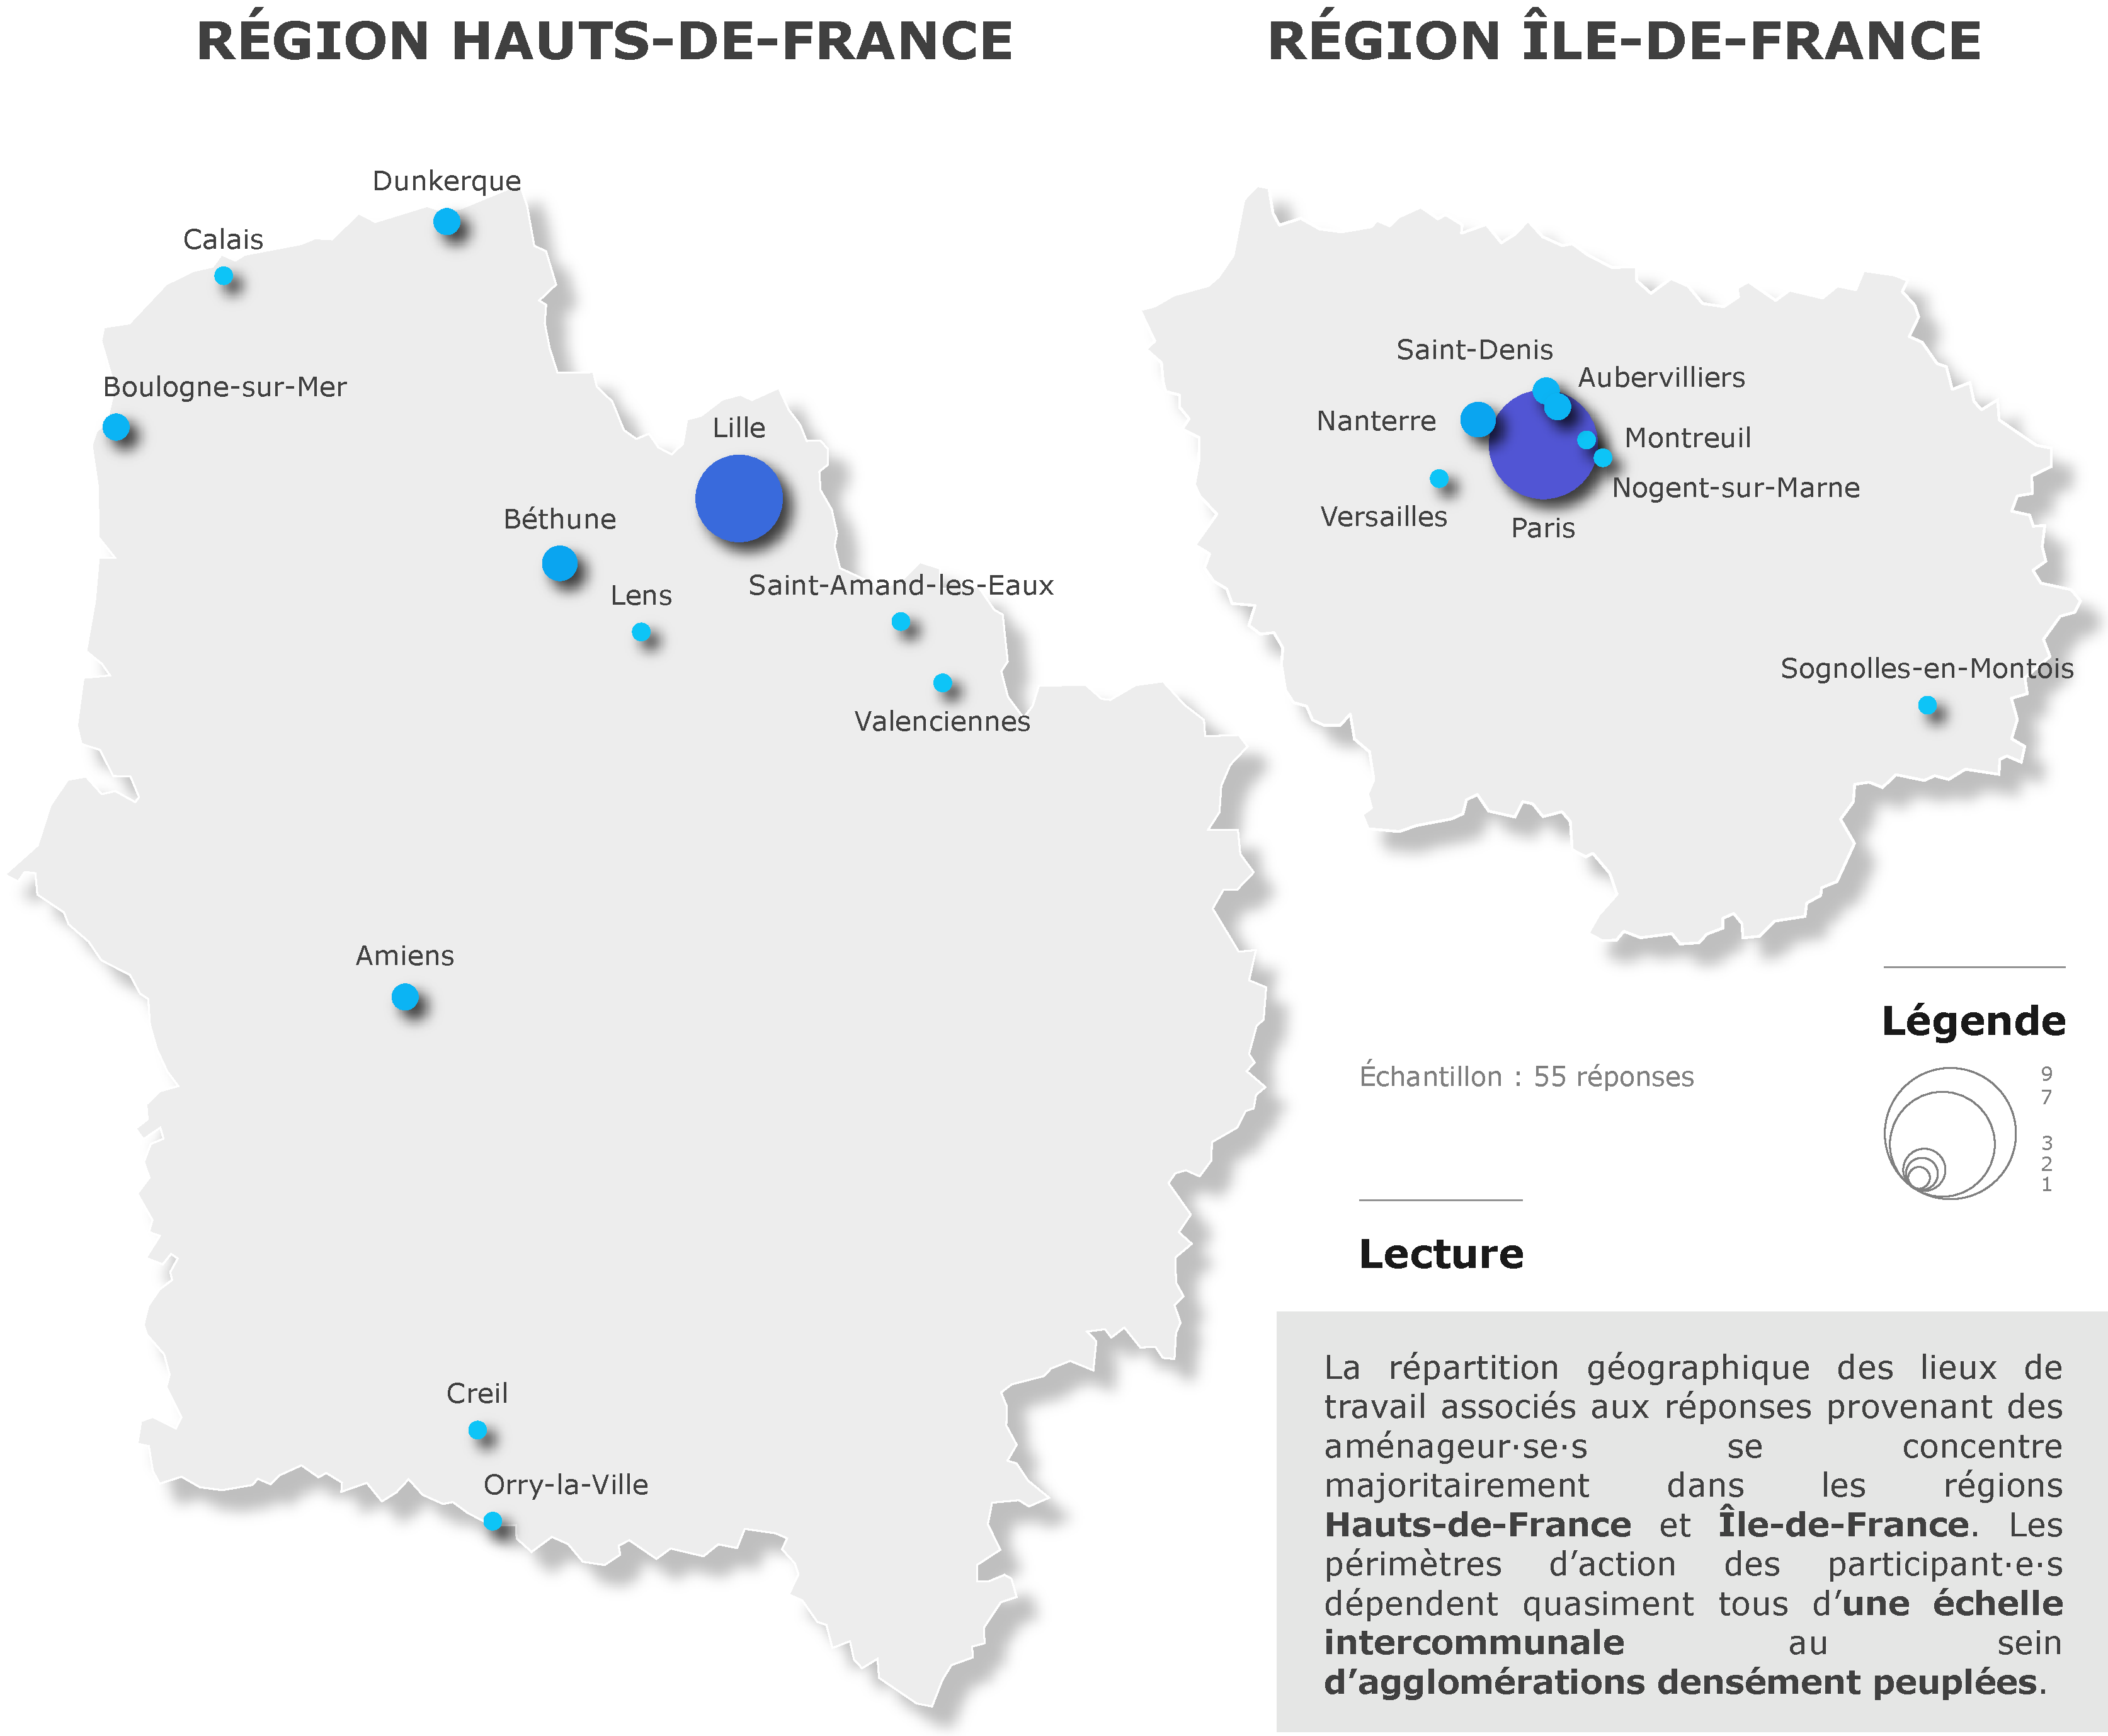
\includegraphics[width=1\columnwidth]{src/Figures/Chap-6/FR_NPART_Carte_lieu_travail_urbanistes.pdf}}
        \vspace{5pt}
        \begin{flushright}\scriptsize{
        Réalisation~: \textcolor{blue}{Dylan Moinse (2024)}
        \\
        Auteur·rice·s~: projet de recherche \acrshort{NPART}
        }\end{flushright}
    \end{carte}

    % Structure et méthode
Dans un premier temps, les participant·e·s ont été appelé·e·s à classer les paramètres prédéfinis dans notre modèle, avant de se voir offrir la possibilité d’en proposer de nouveaux ou de rejeter certains des indices présentés. Enfin, iels ont été enjoint·e·s de détailler leur profil professionnel et personnel. La technique d'aide à la décision multicritère employée repose sur la \acrfull{BWM}, ou la méthode du meilleur et du pire.\footnote{
    La \acrfull{BWM} est une méthode d'évaluation qui permet de recueillir des préférences en invitant les participant·e·s à classer une série d'éléments, qu'iels doivent juger du plus au moins important, en fonction de l'utilité relative perçue. Cette technique a notamment été appliquée par \textcolor{blue}{\textcite[8]{groenendijk_incorporating_2018}}\index{Groenendijk, Laura|pagebf}\index{Rezaei, Jafar|pagebf}\index{Almeida Correia, Gonçalo Homem de|pagebf} dans le cadre du \acrshort{NPM}.
}, et a été développée pour déterminer les poids relatifs des critères, en s'appuyant sur les préférences exprimées par les décideur·se·s. Le·la répondant·e identifie ainsi l'indicateur qu'iel juge le plus important (\Guillemets{le meilleur}) et celui qu'iel estime être le moins pertinent (\Guillemets{le pire}). Cette méthode prend forme à travers une hiérarchisation des facteurs selon les trois axes principaux~: le nœud, le lieu et les connexions. La plate-forme \textsl{LimeSurvey} présente ici l'avantage de proposer une interface interactive, permettant une saisie facilitée des listes de variables. En termes de type d'analyse, l'évaluation a été menée en suivant la méthode \acrshort{IEW}, dans le but de faciliter la comparaison avec la pondération statistique. Afin d’enrichir la nature participative de l'enquête, une série de questions ouvertes a également été intégrée pour encourager les aménageur·se·s à proposer des indicateurs potentiellement absents de la liste initiale et à formuler des recommandations pour mieux guider la réflexion stratégique sur les orientations de notre projet de recherche. Enfin, des questions portant sur la description de leurs formations et de leurs spécialisations, leurs professions, le type et le nom de leurs structures professionnelles, leurs périmètres d'intervention, la durée de leurs expériences professionnelles, ainsi que sur leurs lieux de résidence et de travail et leurs habitudes de mobilité ont été posées.%%Rédigé%%

    % Description de l'échantillon
Au total, 55 réponses ont été recueillies auprès de professionnel·le·s évoluant dans les secteurs de l'urbanisme et, ou bien, de la mobilité, après l'application des processus de nettoyage et de filtrage des données. Parmi elleux, 22 résident et, ou bien, exercent leur activité dans les Hauts-de-France, tandis que 4 résident et, ou bien, travaillent dans un pays limitrophe (voir la \hyperref[fig-chap6:localisation-travail-amenageurs-interroges]{carte~\ref{fig-chap6:localisation-travail-amenageurs-interroges}}, page~\pageref{fig-chap6:localisation-travail-amenageurs-interroges}). La majorité des répondant·e·s se déplace principalement à l'aide des transports en commun, certain·e·s alternant également avec l'usage de la mobilité individuelle légère ou de la marche, ce qui légitime leurs prises de position tant du point de vue de leurs connaissances et de leurs compétences que de celui d’usager·ère·s quotidien·ne·s. Il convient toutefois de préciser que les participant·e·s situé·e·s dans la région étudiée recourent généralement à l’automobile, notamment en dehors de l’agglomération lilloise. À notre connaissance, la constitution d'un échantillon final de 55 répondant·e·s dans le cadre de la pondération des critères pour un \acrshort{NPM} est parmi les plus importantes enquêtes menées à ce jour, surpassant les 30 aménageur·se·s interrogé·e·s par \textcolor{blue}{\textcite[247]{ibrahim_measuring_2023}}\index{Ibrahim, Sara|pagebf}\index{Ayad, Hany|pagebf}\index{Turki, Eslam|pagebf}\index{Saadallah, Dina|pagebf} à Alexandrie ou encore les 36 urbanistes par \textcolor{blue}{\textcite[274]{li_transit_2019}}\index{Li, Zekun|pagebf}\index{Han, Zixuan|pagebf}\index{Xin, Jing|pagebf}\index{Luo, Xin|pagebf}\index{Su, Shiliang|pagebf}\index{Weng, Min|pagebf} à Shanghai.%%Rédigé%%

    % Transition
Après avoir détaillé la méthodologie adoptée pour l'extraction, la validation, la clustérisation et la classification des données, nous nous intéressons désormais aux résultats issus de l'application du \acrshort{NPART}. Afin d'améliorer la lisibilité de l'analyse et de concentrer nos efforts, nous avons choisi de focaliser notre étude sur un cas spécifique, en nous appuyant sur deux typologies précises~: une comparaison des isochrones piétonnes et cyclables (\(PI\) et \(CI\)) en utilisant la méthode \acrshort{IEW} pour la pondération des variables, tout en excluant la pondération définie par les aménageur·se·s. Cette analyse est centrée sur les heures de pointe matinales, afin de capturer les périodes critiques d'utilisation du réseau et de congestion (\(RT_{2}\)), en s'appuyant sur l'algorithme des k-moyennes pour la clustérisation. En concentrant notre attention sur ces paramètres spécifiques, nous visons à offrir des résultats clairs et interprétables. La section suivante présente les résultats obtenus à travers l'application du \acrshort{NPART} dans ces conditions, en discutant des implications des influences relatives de chacun des indicateurs, de la situation des gares et des clusters identifiés.%%Rédigé%%

     % ___________________________________________
    % 6.4.
    \newpage
    \needspace{1\baselineskip} % Réserve de l'espace
    \sectionheader{Potentiel de \textsl{Micromobility-friendly Transit-Oriented Development}}
\section{Potentiel de développement urbain orienté vers le rail et soutenu par la mobilité individuelle légère
    \label{chap6:resultats-modele}
    }

    % Introduction
Une fois les paramètres de calibration du modèle établis et le protocole méthodologique énoncé, nous proposons d’exposer les résultats statistiques issus de son application. Dans un premier temps, nous nous attachons à identifier les critères les plus influents sur l'augmentation du trafic ferroviaire, finalité du \acrshort{TOD}. À partir de cette analyse, nous mettons à jour les composantes prioritaires sur lesquelles les politiques publiques devraient se concentrer pour atteindre l'idée d'un \acrshort{M-TOD} (voir la \hyperref[chap6:results-influence-indicateurs]{section sur la définition d'un urbanisme orienté vers le rail et soutenu par la mobilité individuelle légère}, page~\pageref{chap6:results-influence-indicateurs}). Ensuite, nous procédons à une évaluation de chaque gare et de son environnement urbain, en les positionnant au sein du diagramme prévu par le modèle, afin de déterminer si ces entités se trouvent en situation d’\Guillemets{équilibre} ou, au contraire, présentent un \Guillemets{certain déséquilibre} (voir la \hyperref[chap6:results-caracterisation-gares]{section sur l'évaluation du réseau ferroviaire régionale}, page~\pageref{chap6:results-caracterisation-gares}). Enfin, cette analyse est enrichie par un travail de classification qui permet d’identifier les arrêts stratégiques disposant d’un potentiel d’aménagement (voir la \hyperref[chap6:results-classification-gares]{section sur la classification des gares et des quartiers de gare en fonction des différents périmètres géographiques}, page~\pageref{chap6:results-classification-gares}).%%Rédigé%%

    % 6.4.1.
    \needspace{1\baselineskip} % Réserve de l'espace
\subsection{Influence des paramètres définissant un \textsl{Micromobility-friendly Transit-Oriented Development}
    \label{chap6:results-influence-indicateurs}
    }

    % Introduction
Le concept d’aménagement que nous nous efforçons de formaliser, un \acrfull{M-TOD}, se présente comme une réponse stratégique visant à favoriser l’intégration de la mobilité individuelle légère à l'infrastructure ferroviaire et au système urbain. L’analyse des indicateurs influençant la fréquentation des gares constitue un levier pour comprendre les mécanismes qui sous-tendent leur attractivité et, par extension, leur capacité à impulser des dynamiques positives sur les systèmes de transport et le développement urbain. Cette sous-section explore l’influence des paramètres nodaux, urbains et relatifs à l’accessibilité locale sur la demande de mobilité, tout en intégrant les perceptions des acteur·rice·s de la fabrique urbaine. En croisant les résultats statistiques avec les représentations des aménageur·se·s, l’objectif est de révéler les points de convergence et de divergence, afin de proposer une vision factuelle des priorités à adopter dans les stratégies d’aménagement \acrshort{TOD}.%%Rédigé%%

    % 6.4.1.1.
    \needspace{1\baselineskip} % Réserve de l'espace
\subsubsection*{Effets de la qualité du service ferroviaire sur la demande de mobilité
    \label{chap6:results-influence-indicateurs-node}
    }

    % Influence des indicateurs Node
Du point de vue du niveau de service en gare, l'affluence est principalement déterminée par la fréquence du réseau \acrshort{TGV}, aussi bien durant les jours ouvrables (\(N_{1}\)) que pendant les week-ends (\(N_{2}\)), selon la méthode de pondération par entropie (voir le \hyperref[table-chap6:influence-indicateurs-node]{tableau~\ref{table-chap6:influence-indicateurs-node}}, page~\pageref{table-chap6:influence-indicateurs-node} et l'\hyperref[fig-chap6:resultats-poids-iew-statistiques]{illustration~\ref{fig-chap6:resultats-poids-iew-statistiques}}, page~\pageref{fig-chap6:resultats-poids-iew-statistiques}). Les facteurs liés à la fréquence des liaisons ferroviaires (de \(N_{1}\) à \(N_{4}\)) figurent également de manière prépondérante dans les critères évalués par les urbanistes. Viennent ensuite la connectivité des gares au sein du réseau, apprécié à travers la centralité de proximité (\(N_{11}\)) et le degré de centralité (\(N_{9}\)), qui influencent positivement la fréquentation des gares. À l'inverse, l'étendue des horaires de service (\(N_{5}\) et \(N_{6}\)), ainsi que l'accès aux centralités urbaines (de \(N_{13}\) à \(N_{16}\)) et la centralité d'intermédiarité (\(N_{10}\)), exercent une influence moindre, bien que leur importance soit surévaluée par les aménageur·se·s. Par ailleurs, ces dernier·ère·s mettent peu en avant le nombre de dessertes par gare (\(N_{8}\)) ni le degré de centralité (\(N_{9}\)), bien que ce soient des indicateurs clés.%%Rédigé%%

    % Tableau Influence des indicateurs Node
% Tableau Influence des indicateurs Node
%%Rédigé%%
    \begin{table}[h!]
    \centering
    \renewcommand{\arraystretch}{1.5}
    \resizebox{\columnwidth}{!}{
    \begin{tabular}{p{0.08\columnwidth}p{0.5\columnwidth}p{0.21\columnwidth}p{0.21\columnwidth}}
        %\hline
    \rule{0pt}{15pt} \small{\textbf{\textcolor{blue}{ID}}} & \small{\textbf{\textcolor{blue}{Indicateur}}} & \small{\textbf{\textcolor{blue}{Statistiques}}} & \small{\textbf{\textcolor{blue}{Perception}}}\\
        \hline
\small{\(N_{1}\)} & \small{Fréquence du réseau \acrshort{TGV}, en semaine} & \underline{\small{\textbf{0,264}} (2\textsuperscript{e})} & \underline{\small{\textbf{0,375}} (1-4\textsuperscript{e})}\\
\small{\(N_{2}\)} & \small{Fréquence du réseau \acrshort{TGV}, le week-end} & \underline{\small{\textbf{0,266}} (1\textsuperscript{er})} & \underline{\small{\textbf{0,375}} (1-4\textsuperscript{e})}\\
\small{\(N_{3}\)} & \small{Fréquence du réseau \acrshort{TER}, en semaine} & \small{\textbf{0,034} (7\textsuperscript{e})} & \underline{\small{\textbf{0,375}} (1-4\textsuperscript{e})}\\
\small{\(N_{4}\)} & \small{Fréquence du réseau \acrshort{TER}, le week-end} & \small{\textbf{0,039} (6\textsuperscript{e})} & \underline{\small{\textbf{0,375}} (1-4\textsuperscript{e})}\\
\small{\(N_{5}\)} & \small{Amplitude horaire, en semaine} & \small{\textbf{0,001} (16\textsuperscript{e})} & \small{\textbf{0,082} (11-12\textsuperscript{e})}\\
\small{\(N_{6}\)} & \small{Amplitude horaire, le week-end} & \small{\textbf{0,009} (14\textsuperscript{e})} & \small{\textbf{0,082} (11-12\textsuperscript{e})}\\
\small{\(N_{7}\)} & \small{Vitesse commerciale} & \small{\textbf{0,015} (9\textsuperscript{e})} & \small{\textbf{0,067} (14\textsuperscript{e})}\\
\small{\(N_{8}\)} & \small{Nombre de directions} & \small{\textbf{0,068} (5\textsuperscript{e})} & \small{\textbf{0,035} (16\textsuperscript{e})}\\
\small{\(N_{9}\)} & \small{Degré de centralité} & \underline{\small{\textbf{0,077}} (4\textsuperscript{e})} & \small{\textbf{0,057} (15\textsuperscript{e})}\\
\small{\(N_{10}\)} & \small{Centralité d'intermédiarité} & \small{\textbf{0,011} (12\textsuperscript{e})} & \small{\textbf{0,134} (5\textsuperscript{e})}\\
\small{\(N_{11}\)} & \small{Centralité de proximité} & \underline{\small{\textbf{0,152}} (3\textsuperscript{e})} & \small{\textbf{0,093} (6\textsuperscript{e})}\\
\small{\(N_{12}\)} & \small{Nombre de stations accessibles en une heure} & \small{\textbf{0,019} (8\textsuperscript{e})} & \small{\textbf{0,067} (13\textsuperscript{e})}\\
\small{\(N_{13}\)} & \small{Nombre de stations pour accéder à Euralille} & \small{\textbf{0,010} (13\textsuperscript{e})} & \small{\textbf{0,090} (7-10\textsuperscript{e})}\\
\small{\(N_{14}\)} & \small{Temps de trajet pour accéder à Euralille} & \small{\textbf{0,014} (10\textsuperscript{e})} & \small{\textbf{0,090} (7-10\textsuperscript{e})}\\
\small{\(N_{15}\)} & \small{Nombre de stations pour accéder à Châtelet} & \small{\textbf{0,014} (11\textsuperscript{e})} & \small{\textbf{0,090} (7-10\textsuperscript{e})}\\
\small{\(N_{16}\)} & \small{Temps de trajet pour accéder à Châtelet} & \small{\textbf{0,007} (15\textsuperscript{e})} & \small{\textbf{0,090} (7-10\textsuperscript{e})}\\
        \hline
        \end{tabular}}
    \caption{Influence relative, par entropie, des indicateurs indépendants, liés au niveau de service (\(N\)), sur la fréquentation des gares.}
    \label{table-chap6:influence-indicateurs-node}
        \vspace{5pt}
        \begin{flushleft}\scriptsize{
        \textcolor{blue}{Lecture~:} la fréquence du réseau \acrshort{TGV}, le week-end, (\(N_{2}\)) explique statistiquement 20,6~\% de la fréquentation des gares, contre 37,5~\% selon les aménageur·se·s.
        }\end{flushleft}
        \begin{flushright}\scriptsize{
        Réalisation~: \textcolor{blue}{Dylan Moinse (2024)}
        \\
        Auteur·rice·s~: projet de recherche \acrshort{NPART}
        }\end{flushright}
        \end{table}%%Rédigé%%

    % Littérature
À la lumière des modèles \acrshort{NPM} antérieurs, \textcolor{blue}{\textcite[8]{cummings_does_2022}}\index{Cummings, Christopher|pagebf}\index{Mahmassani, Hani|pagebf} ont établi que le nombre de services \textsl{Amtrak} par semaine, aux États-Unis, constitue la variable la plus influente dans les divers scénarios analysés. De manière similaire, \textcolor{blue}{\textcite[5]{caset_integrating_2020}}\index{Caset, Freke|pagebf}\index{Blainey, Simon|pagebf}\index{Derudder, Ben|pagebf}\index{Boussauw, Kobe|pagebf}\index{Witlox, Frank|pagebf} ont observé qu'une augmentation de 1~\% de la fréquence des \acrshort{TER} en Flandre, en Belgique, se traduit par une hausse de 0,6~\% de la fréquentation du réseau ferroviaire. Cependant, ces dernier·ère·s ont également déterminé que le degré de centralité est un indicateur encore plus déterminant~: une hausse de 1~\% de sa valeur tend à accroître la fréquentation des gares de 2~\%. À cet effet, \textcolor{blue}{\textcite[11]{amini_pishro_node_2022}}\index{Amini Pishro, Ahad|pagebf}\index{L'Hostis, Alain|pagebf}\index{Chen, Dong|pagebf}\index{Chen, Mojdeh|pagebf}\index{Amini Pishro, Mojdeh|pagebf}\index{Zhang, Zhengrui|pagebf}\index{Li, Jun|pagebf}\index{Zhao, Yuandi|pagebf}\index{Zhang, Lili|pagebf} ont identifié le degré de centralité parmi les sept indicateurs les plus influents pour stimuler le volume de voyageur·se·s à Chengdu, en Chine. De manière analogue, \textcolor{blue}{\textcite[9]{cao_coordination_2020}}\index{Cao, Zhejing|pagebf}\index{Asakura, Yasuo|pagebf}\index{Tan, Zongbo|pagebf} ont mis en évidence le degré de centralité, ainsi que le nombre de lignes \textsl{express}, comme les deux variables les plus déterminants afin d'intensifier les flux à Tokyo, au Japon.%%Rédigé%%

    % Figure Pondération IEW statistiques
    \begin{figure}[h!]\vspace*{4pt}
        \caption{Influence statistique des indicateurs sur la fréquentation des gares, à l'échelle piétonne et cyclable.}
        \label{fig-chap6:resultats-poids-iew-statistiques}
        \centerline{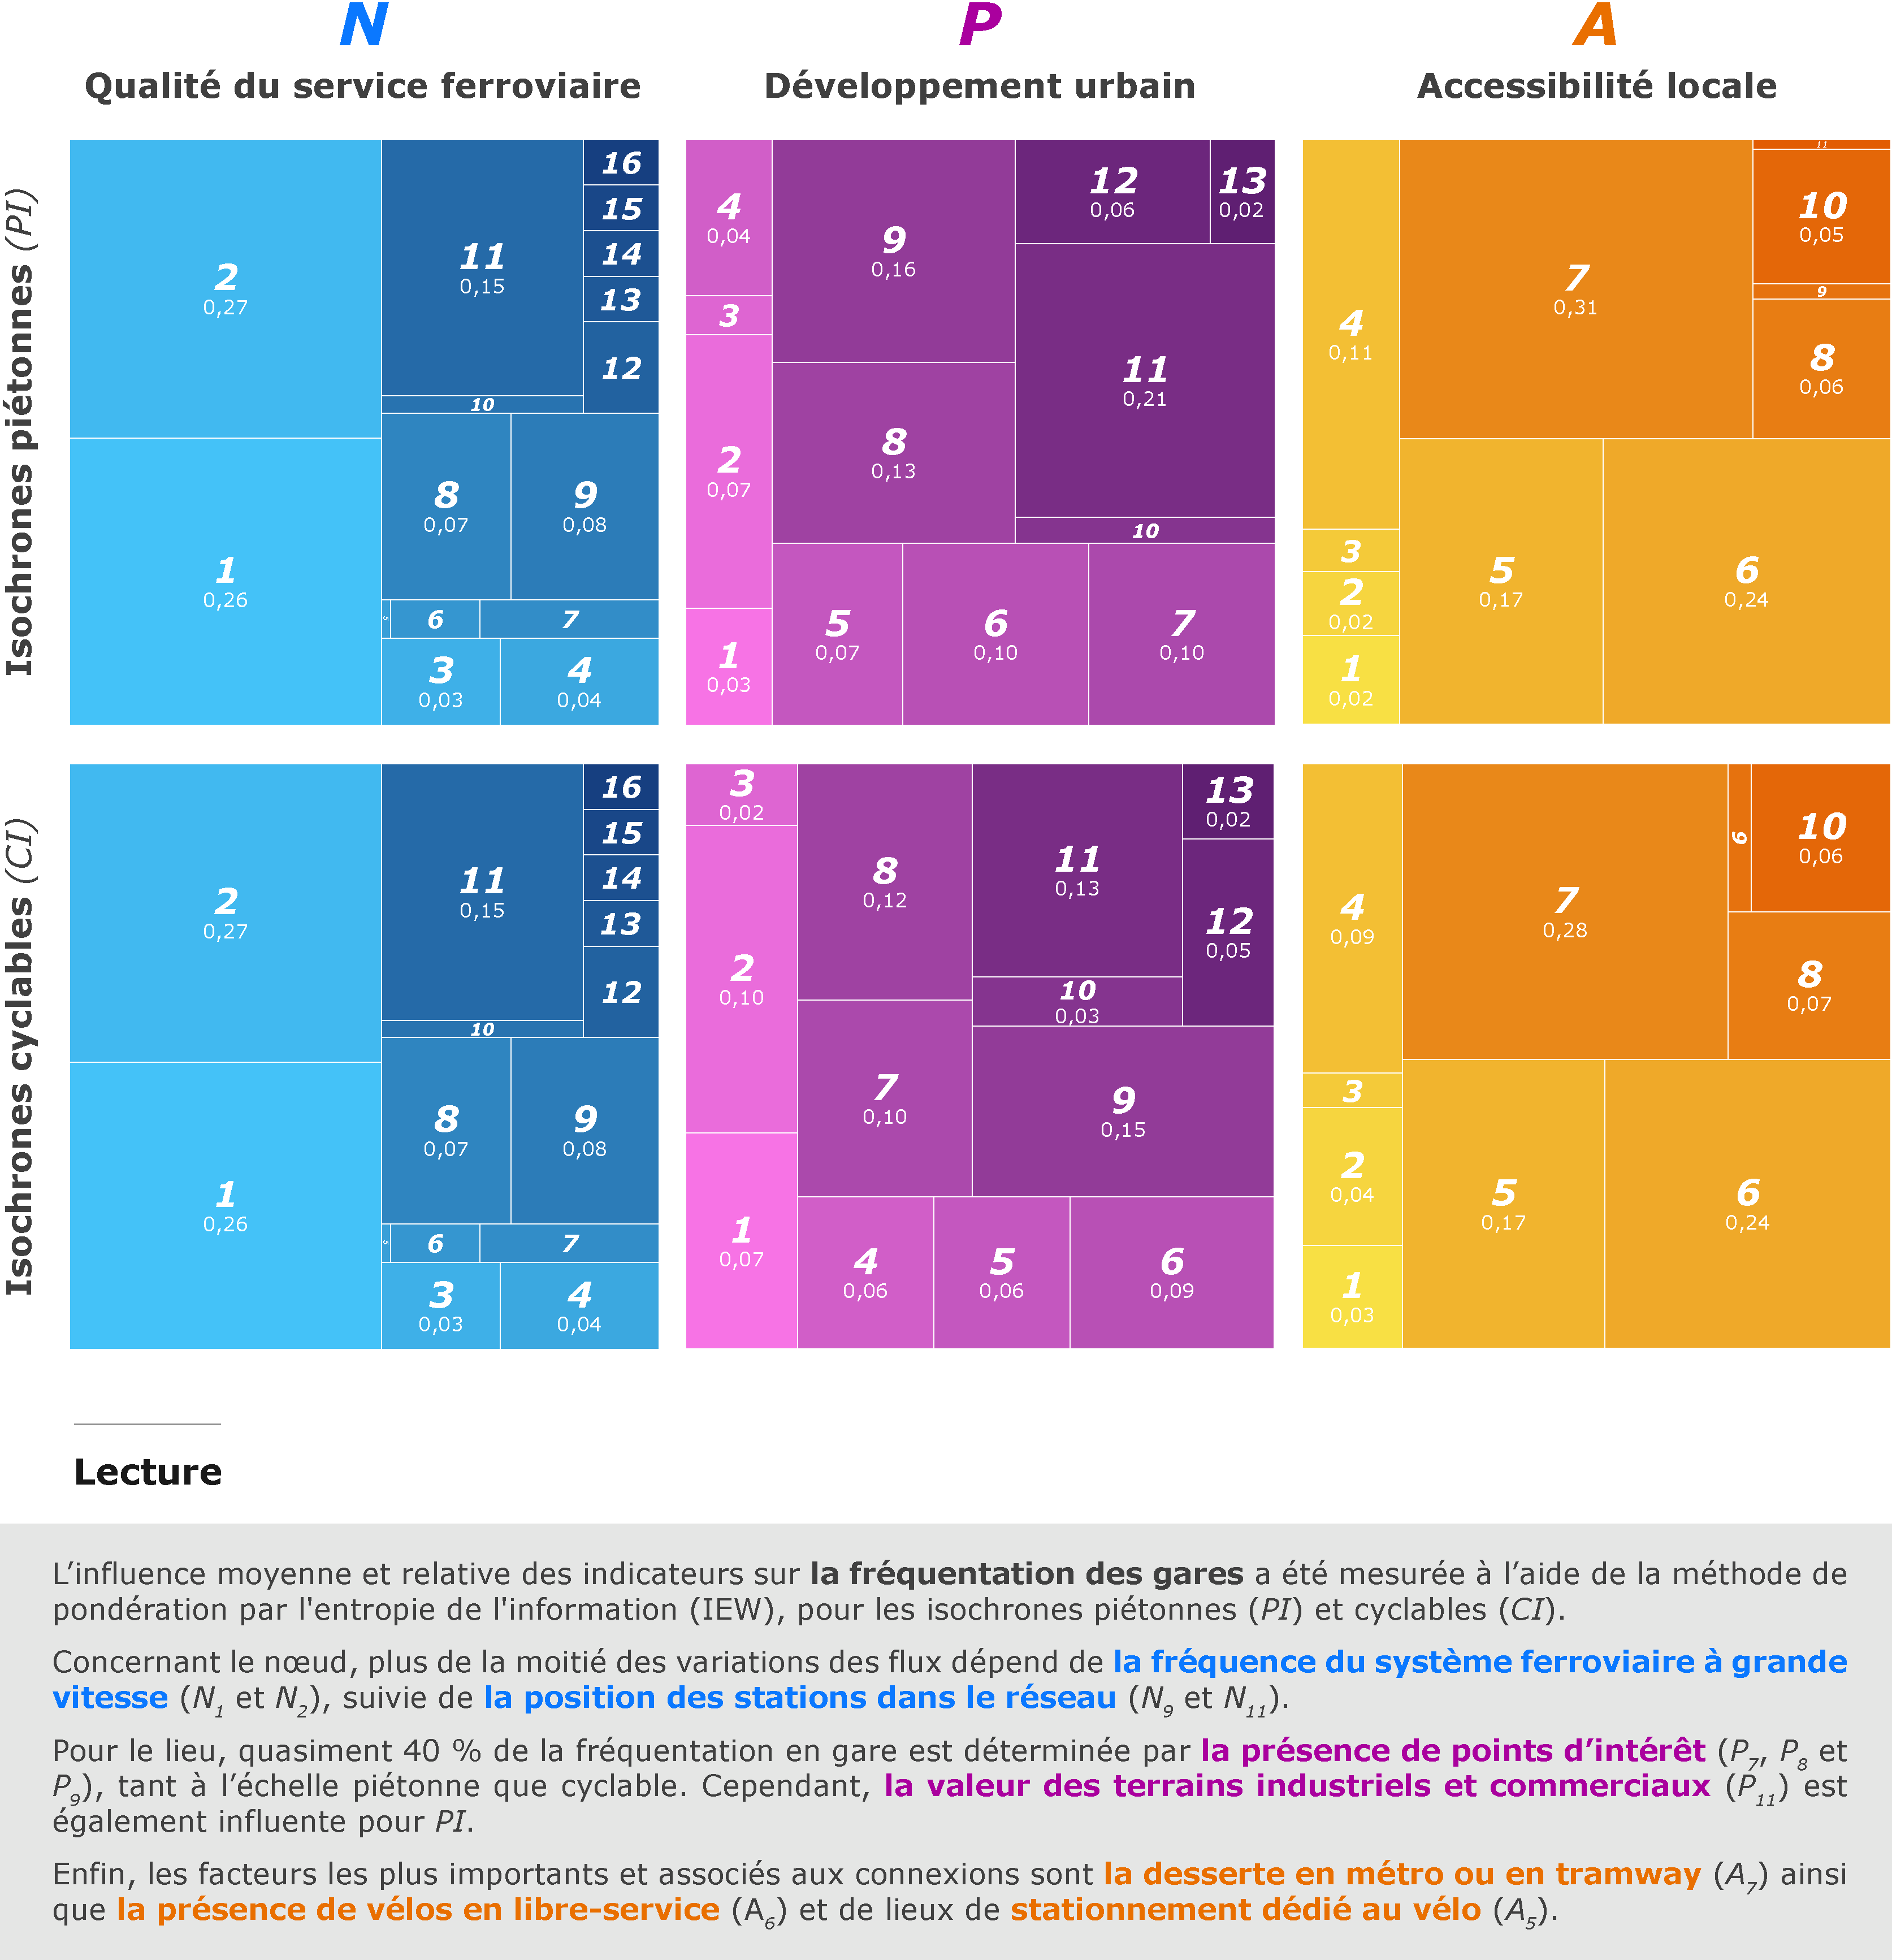
\includegraphics[width=1\columnwidth]{src/Figures/Chap-6/FR_NPART_Poids_Statistiques_IEW_Indicateurs.pdf}}
        \vspace{5pt}
        \begin{flushright}\scriptsize{
        Réalisation~: \textcolor{blue}{Dylan Moinse (2024)}
        \\
        Auteur·rice·s~: projet de recherche \acrshort{NPART}
        }\end{flushright}
    \end{figure}

    % Discussion influence des indicateurs Node
La fonction primordiale de la fréquence des liaisons ferroviaires, tant statistiquement qu'en termes d'objectifs de planification, illustre combien cet indicateur est en mesure de renforcer l'attractivité des gares. Parallèlement, la position stratégique du nœud au sein des réseaux, mise en évidence par le besoin d'une centralité de proximité et d'un degré de centralité relativement importants, souligne l'importance des connexions dans le réseau. En effet, la centralité de proximité indique que la gare est située à proximité immédiate de divers points nodaux, facilitant ainsi les déplacements intermodaux, tandis que le degré de centralité confirme le rôle de la gare comme nœud essentiel du réseau de transport. Notons que l'analyse statistique met en avant l'importance degré de centralité, tandis que les professionnel·le·s de l'aménagement et du transport lui accordent une place moindre. À l'inverse, la mesure de l'intermédiarité, jouant alors un rôle secondaire, est surévaluée par ces mêmes acteur·rice·s, qui la considèrent comme un facteur bien plus déterminant. Ces observations soulignent le rôle de la notion de \Guillemets{réseau} dans les dynamiques du \acrshort{TOD}~: cela invite à ne pas limiter la question du \acrshort{TOD} à la seule proximité autour de chaque gare, à savoir son environnement urbain immédiat, comme pourraient le laisser penser la lecture de certaines analyses réductrices \textcolor{blue}{\autocite[10]{cerema_articuler_2015}}\index{Cerema@\textsl{Cerema}|pagebf}. Au contraire, il convient d'adopter une approche multi-échelles, prenant simultanément en compte les différentes dimensions spatiales du réseau de transport et du système urbain \textcolor{blue}{\textcite[11]{cervero_transit_1998}}\index{Cervero, Robert|pagebf}. Le décalage entre l’évaluation des acteur·rice·s et l’impact réel du réseau ferroviaire sur la fréquentation des gares, ainsi que leur tendance à surestimer le rôle de l’intermédiarité du réseau ferré, font écho aux conclusions de la thèse de doctorat réalisée par \textcolor{blue}{Wendy} \textcolor{blue}{\autocite[79]{tan_pursuing_2013}}\index{Tan, Wendy|pagebf}\index{Bertolini, Luca|pagebf}\index{Janssen-Jansen, Leonie|pagebf} sur le \Guillemets{manque de connaissance des spécificités des transports publics par les urbanistes} (\textsl{culture of public transport is missing}. Nous pouvons en tirer la conclusion que les principaux facteurs expliquant l'affluence d'une gare impliquent le renforcement de leur \Guillemets{nodalité}\footnote{
    Le concept de \Guillemets{nodalité} désigne \Guillemets{\textsl{l'ensemble des caractères relevant de la morphologie, des fonctionnements et des dynamiques des nœuds de transports} [\dots]} \textcolor{blue}{\autocite[5]{bavoux_nodalite_2005}}\index{Bavoux, Jean-Jacques|pagebf}. L'auteur propose par ailleurs le terme de \Guillemets{nodosité} pour décrire les divers phénomènes d'agrégation qui peuvent accompagner une nodalité circulatoire \textcolor{blue}{\autocite[13]{bavoux_nodalite_2005}}\index{Bavoux, Jean-Jacques|pagebf}.
} relevant d'interactions entre la centralité, l'accessibilité et l'attractivité, à différentes échelles \textcolor{blue}{\autocite[13]{bavoux_nodalite_2005}}\index{Bavoux, Jean-Jacques|pagebf}. Il incombe ainsi aux gestionnaires d'infrastructure de mobilité de veiller à une intégration optimale des gares dans le réseau ferroviaire régional. Cette intégration pourrait impliquer la maximisation de la fréquence des liaisons et l'amélioration de la connectivité des gares.%%Rédigé%%

    % 6.4.1.2.
    \needspace{1\baselineskip} % Réserve de l'espace
\subsubsection*{Effets du degré de développement urbain sur la demande de mobilité
    \label{chap6:results-influence-indicateurs-place}
    }

    % Influence des indicateurs Place
Sur le plan statistique, les indicateurs de développement urbain exerçant la plus grande influence sur la fréquentation des gares comprennent la valeur des biens immobiliers destinés aux activités commerciales et industrielles (\(P_{11}\)), les \acrshort{POIs} de catégories \Guillemets{supérieurs} et \Guillemets{intermédiaires} (\(P_{9}\) et \(P_{8}\)), l'usage du sol pour les espaces verts (\(P_{6}\)) et la densité d'emploi (\(P_{2}\)), comme l'illustrent le \hyperref[table-chap6:influence-indicateurs-place]{tableau~\ref{table-chap6:influence-indicateurs-place}} (page~\pageref{table-chap6:influence-indicateurs-place}) et l'\hyperref[fig-chap6:resultats-poids-iew-statistiques]{illustration~\ref{fig-chap6:resultats-poids-iew-statistiques}} (page~\pageref{fig-chap6:resultats-poids-iew-statistiques}). En pratique, une distinction s'opère entre les périmètres piétons (\(PI\)) et cyclables (\(CI\)) des gares, avec un rôle plus important des densités d'emploi et de la population (\(P_{1}\)) pour l'\Guillemets{aire secondaire}. Du point de vue des aménageur·se·s, l'occupation des sols à dominante commerciale (\(P_{4}\)) ainsi que la présence d'équipements et de services (de \(P_{7}\) à \(P_{9}\)) sont considérés comme primordiaux. À l'inverse, la valeur foncière des terrains reçoit peu d'attention de la part des acteurs de la fabrique urbaine, ce qui révèle une valorisation marquée de la fonction commerciale et de services en termes d'intégration urbaine, mais également une tendance à sous-estimer l'importance de la valeur immobilière.%%Rédigé%%

    % Tableau Influence des indicateurs Place
% Tableau Influence des indicateurs Place
%%Rédigé%%
    \begin{table}[h!]
    \centering
    \renewcommand{\arraystretch}{1.5}
    \resizebox{\columnwidth}{!}{
    \begin{tabular}{p{0.08\columnwidth}p{0.38\columnwidth}p{0.18\columnwidth}p{0.18\columnwidth}p{0.18\columnwidth}}
        %\hline
    \rule{0pt}{15pt} \small{\textbf{\textcolor{blue}{ID}}} & \small{\textbf{\textcolor{blue}{Indicateur}}} & \small{\textbf{\textcolor{blue}{\(PI\)*}}} & \small{\textbf{\textcolor{blue}{\(CI\)*}}} & \small{\textbf{\textcolor{blue}{Perception}}}\\
        \hline
\small{\(P_{1}\)} & \small{Densité de population} & \small{\textbf{0,035} (10\textsuperscript{e})} & \small{\textbf{0,072} (7\textsuperscript{e})} & \small{\textbf{0,097} (7\textsuperscript{e})}\\
\small{\(P_{2}\)} & \small{Densité d'emploi} & \small{\textbf{0,068} (7\textsuperscript{e})} & \underline{\small{\textbf{0,104}} (4\textsuperscript{e})} & \small{\textbf{0,102} (6\textsuperscript{e})}\\
\small{\(P_{3}\)} & \small{Fonction résidentielle} & \small{\textbf{0,007} (13\textsuperscript{e})} & \small{\textbf{0,023} (12\textsuperscript{e})} & \small{\textbf{0,087} (11\textsuperscript{e})}\\
\small{\(P_{4}\)} & \small{Fonction commerciale} & \small{\textbf{0,039} (9\textsuperscript{e})} & \small{\textbf{0,062} (9\textsuperscript{e})} & \underline{\small{\textbf{0,119}} (1\textsuperscript{er})}\\
\small{\(P_{5}\)} & \small{Fonction industrielle et de bureaux} & \small{\textbf{0,070} (6\textsuperscript{e})} & \small{\textbf{0,062} (8\textsuperscript{e})} & \small{\textbf{0,089} (10\textsuperscript{e})}\\
\small{\(P_{6}\)} & \small{Présence d'espaces verts} & \underline{\small{\textbf{0,096}} (4\textsuperscript{e})} & \small{\textbf{0,094} (6\textsuperscript{e})} & \small{\textbf{0,105} (5\textsuperscript{e})}\\
\small{\(P_{7}\)} & \small{\acrshort{POIs} de \Guillemets{proximité}} & \small{\textbf{0,096} (5\textsuperscript{e})} & \small{\textbf{0,096} (5\textsuperscript{e})} & \underline{\small{\textbf{0,115}} (2-4\textsuperscript{e})}\\
\small{\(P_{8}\)} & \small{\acrshort{POIs} \Guillemets{intermédiaires}} & \underline{\small{\textbf{0,131}} (3\textsuperscript{e})} & \underline{\small{\textbf{0,118}} (3\textsuperscript{e})} & \underline{\small{\textbf{0,115}} (2-4\textsuperscript{e})}\\
\small{\(P_{9}\)} & \small{\acrshort{POIs} \Guillemets{supérieurs}} & \underline{\small{\textbf{0,160}} (2\textsuperscript{e})} & \underline{\small{\textbf{0,153}} (1\textsuperscript{er})} & \underline{\small{\textbf{0,115}} (2-4\textsuperscript{e})}\\
\small{\(P_{10}\)} & \small{Valeur des lieux résidentiels} & \small{\textbf{0,018} (11\textsuperscript{e})} & \small{\textbf{0,026} (11\textsuperscript{e})} & \small{\textbf{0,094} (8\textsuperscript{e})}\\
\small{\(P_{11}\)} & \small{Valeur des lieux d'activité} & \underline{\small{\textbf{0,206}} (1\textsuperscript{er})} & \underline{\small{\textbf{0,130}} (2\textsuperscript{e})} & \small{\textbf{0,012} (13\textsuperscript{e})}\\
\small{\(P_{12}\)} & \small{Part de logements sociaux} & \small{\textbf{0,055} (8\textsuperscript{e})} & \small{\textbf{0,046} (10\textsuperscript{e})} & \small{\textbf{0,092} (9\textsuperscript{e})}\\
\small{\(P_{13}\)} & \small{Revenu moyen des ménages} & \small{\textbf{0,018} (12\textsuperscript{e})} & \small{\textbf{0,016} (13\textsuperscript{e})} & \small{\textbf{0,087} (12\textsuperscript{e})}\\
        \hline
        \end{tabular}}
    \caption{Influence relative, par entropie, des indicateurs indépendants, liés à l'insertion urbaine (\(P\)), sur la fréquentation des gares.}
    \label{table-chap6:influence-indicateurs-place}
        \vspace{5pt}
        \begin{flushleft}\scriptsize{
        \textcolor{blue}{Note~:} les statistiques \(PI\) et \(CI\) correspondent aux valeurs propres aux isochrones piétonnes et cyclables.
        \\
        \textcolor{blue}{Lecture~:} la valeur foncière des lieux d'activité (\(P_{11}\)) explique statistiquement 20,6~\% et 13,0~\% de la fréquentation des gares, pour les périmètres piétons (\(PI\)) et cyclables (\(CI\)). Les effets attendus de cette variable s'élèvent seulement à 1,2~\% selon les aménageur·se·s.
        }\end{flushleft}
        \begin{flushright}\scriptsize{
        Réalisation~: \textcolor{blue}{Dylan Moinse (2024)}
        \\
        Auteur·rice·s~: projet de recherche \acrshort{NPART}
        }\end{flushright}
        \end{table}%%Rédigé%%

    % Littérature
Ces résultats sont en accord avec les observations d'\textcolor{blue}{\textcite[11]{amini_pishro_node_2022}}\index{Amini Pishro, Ahad|pagebf}\index{Yang, Qihong|pagebf}\index{Zhang, Shiquan|pagebf}\index{Amini Pishro, Mojdeh|pagebf}\index{Zhang, Zhengrui|pagebf}\index{Zhao, Yana|pagebf}\index{Postel, Victor|pagebf}\index{Huang, Dengshi|pagebf}\index{Li, WeiYu|pagebf} qui indiquent que le prix moyen des terrains commerciaux et de bureaux est positivement corrélé à la fréquentation des gares. En revanche, nos résultats divergent de ceux rapportés par \textcolor{blue}{\textcite[9]{cummings_does_2022}}\index{Cummings, Christopher|pagebf}\index{Mahmassani, Hani|pagebf}, qui notent une corrélation positive entre le prix des logements autour des gares et la fréquentation de celles-ci aux États-Unis. Quant aux \acrshort{POIs}, \textcolor{blue}{\textcite[5]{pezeshknejad_evaluating_2020}}\index{Pezeshknejad, Parsa|pagebf}\index{Monajem, Saeed|pagebf}\index{Mozafari, Hamid|pagebf} constatent que les zones autour des arrêts de \acrshort{BHNS} qui concentrent un grand nombre de \acrshort{POIs} attirent davantage de voyageur·se·s à Téhéran, en Iran. De manière plus générale, l'utilisation des sols à dominante commerciale et de bureaux, ainsi que la densité d'emploi, tendent à augmenter la fréquentation des services \textsl{Amtrack} \textcolor{blue}{\autocite[8]{cummings_does_2022}}\index{Cummings, Christopher|pagebf}\index{Mahmassani, Hani|pagebf}.%%Rédigé%%

    % Discussion influence des indicateurs Place
L'examen des indicateurs de développement urbain qui influencent la fréquentation des gares met en exergue le rôle joué par l'intégration urbaine et économique des gares et de leurs environs dans le cadre du \acrshort{M-TOD}. Les propriétés immobilières à usage commercial et industriel, conjointement à la présence renforcée de \acrshort{POIs} et à la densité d'emploi, se révèlent être des moteurs substantiels de l'attractivité des gares. Toutefois, le faible intérêt porté à la valeur foncière des terrains soulève des questions et indique un déséquilibre potentiel dans la considération des facteurs immobiliers. Les expert·e·s identifient la fonction commerciale, tandis que l'analyse statistique privilégie les valeurs foncières des lieux d'activité. Une telle sous-évaluation par les acteur·rice·s pourrait masquer des opportunités de mise en valeur et de financement des infrastructures de transport et du traitement des espaces publics, éléments clés de la troisième dimension du \acrshort{NPART}.%%Rédigé%%

    % 6.4.1.3.
    \needspace{1\baselineskip} % Réserve de l'espace
\subsubsection*{Effets de la gestion des espaces publics et de l'accessibilité locale sur la demande de mobilité
    \label{chap6:results-influence-indicateurs-accessibility}
    }

    % Influence des indicateurs Accessibility
En ce qui concerne la gestion des espaces publics et l'accessibilité locale, statistiquement, ce sont principalement la problématique des \Guillemets{premiers et derniers kilomètres} qui influencent majoritairement la fréquentation des gares, comme le montrent le \hyperref[table-chap6:influence-indicateurs-accessibility]{tableau~\ref{table-chap6:influence-indicateurs-accessibility}} (page~\pageref{table-chap6:influence-indicateurs-accessibility}) et l'\hyperref[fig-chap6:resultats-poids-iew-statistiques]{illustration~\ref{fig-chap6:resultats-poids-iew-statistiques}} (page~\pageref{fig-chap6:resultats-poids-iew-statistiques}). Nous retrouvons plus précisément la desserte des réseaux de transport en commun urbains sur rail (\(A_{7}\)) et trois aspects majeurs de ce qui compose le \Guillemets{système vélo} \textcolor{blue}{\autocites[169]{heran_retour_2015}[]{heran_systeme_2001}}\index{Héran, Frédéric|pagebf}, c'est-à-dire la présence de services \acrshort{VLS} (\(A_{6}\)) ainsi que l'aménagement de lieux de stationnement vélo (\(A_{5}\)) et d'un réseau cyclable (\(A_{4}\)). Ces résultats statistiques mettent alors au premier plan le rôle stratégique de l'\gls{intermodalité} dans l'attractivité du réseau ferroviaire, et des gares à l'échelle locale. Ces observations sont suivies par les réponses recueillies des experts locaux qui ont hiérarchisé l'importance du réseau piéton (\(A_{1}\)), du stationnement vélo (\(A_{5}\)), de la vitesse motorisée (\(A_{9}\)) et de la desserte en métro et en tramway (\(A_{7}\)).

    % Tableau Influence des indicateurs Accessibility
% Tableau Influence des indicateurs Accessibility
%%Rédigé%%
    \begin{table}[h!]
    \centering
    \renewcommand{\arraystretch}{1.5}
    \resizebox{\columnwidth}{!}{
    \begin{tabular}{p{0.08\columnwidth}p{0.38\columnwidth}p{0.18\columnwidth}p{0.18\columnwidth}p{0.18\columnwidth}}
        %\hline
    \rule{0pt}{15pt} \small{\textbf{\textcolor{blue}{ID}}} & \small{\textbf{\textcolor{blue}{Indicateur}}} & \small{\textbf{\textcolor{blue}{\(PI\)*}}} & \small{\textbf{\textcolor{blue}{\(CI\)*}}} & \small{\textbf{\textcolor{blue}{Perception}}}\\
        \hline
\small{\(A_{1}\)} & \small{Réseau piéton} & \small{\textbf{0,025} (7\textsuperscript{e})} & \small{\textbf{0,027} (8\textsuperscript{e})} & \underline{\small{\textbf{0,120}} (1\textsuperscript{er})}\\
\small{\(A_{2}\)} & \small{Densité d'intersection} & \small{\textbf{0,018} (8\textsuperscript{e})} & \small{\textbf{0,037} (7\textsuperscript{e})} & \small{\textbf{0,086} (7\textsuperscript{e})}\\
\small{\(A_{3}\)} & \small{Taux d'efficacité spatiale} & \small{\textbf{0,012} (9\textsuperscript{e})} & \small{\textbf{0,009} (10\textsuperscript{e})} & \small{\textbf{0,041} (11\textsuperscript{e})}\\
\small{\(A_{4}\)} & \small{Réseau cyclable} & \underline{\small{\textbf{0,110}} (4\textsuperscript{e})} & \underline{\small{\textbf{0,085}} (4\textsuperscript{e})} & \small{\textbf{0,086} (8\textsuperscript{e})}\\
\small{\(A_{5}\)} & \small{Stationnement vélo} & \underline{\small{\textbf{0,169}} (3\textsuperscript{e})} & \underline{\small{\textbf{0,171}} (3\textsuperscript{e})} & \underline{\small{\textbf{0,115}} (2\textsuperscript{e})}\\
\small{\(A_{6}\)} & \small{Services de \acrshort{VLS}} & \underline{\small{\textbf{0,239}} (2\textsuperscript{e})} & \underline{\small{\textbf{0,244}} (2\textsuperscript{e})} & \small{\textbf{0,084} (9\textsuperscript{e})}\\
\small{\(A_{7}\)} & \small{Services de métro et de tramway} & \underline{\small{\textbf{0,307}} (1\textsuperscript{er})} & \underline{\small{\textbf{0,284}} (1\textsuperscript{er})} & \underline{\small{\textbf{0,097}} (4\textsuperscript{e})}\\
\small{\(A_{8}\)} & \small{Services de \acrshort{BHNS} et de bus} & \small{\textbf{0,056} (5\textsuperscript{e})} & \small{\textbf{0,068} (5\textsuperscript{e})} & \small{\textbf{0,081} (10\textsuperscript{e})}\\
\small{\(A_{9}\)} & \small{Vitesse motorisée} & \small{\textbf{0,006} (10\textsuperscript{e})} & \small{\textbf{0,009} (9\textsuperscript{e})} & \underline{\small{\textbf{0,106}} (3\textsuperscript{e})}\\
\small{\(A_{10}\)} & \small{Stationnement automobile} & \small{\textbf{0,054} (6\textsuperscript{e})} & \small{\textbf{0,064} (6\textsuperscript{e})} & \small{\textbf{0,094} (5\textsuperscript{e})}\\
\small{\(A_{11}\)} & \small{Taux de motorisation} & \small{\textbf{0,004} (11\textsuperscript{e})} & \small{\textbf{0,003} (11\textsuperscript{e})} & \small{\textbf{0,088} (6\textsuperscript{e})}\\
        \hline
        \end{tabular}}
    \caption{Influence relative, par entropie, des indicateurs indépendants, liés à l'accessibilité locale (\(A\)), sur la fréquentation des gares.}
    \label{table-chap6:influence-indicateurs-accessibility}
        \vspace{5pt}
        \begin{flushleft}\scriptsize{
        \textcolor{blue}{Note~:} les statistiques \(PI\) et \(CI\) correspondent aux valeurs propres aux isochrones piétonnes et cyclables.
        \\
        \textcolor{blue}{Lecture~:} la desserte en métro et en tramway (\(A_{7}\)) explique statistiquement 30,7~\% et 28,4~\% de la fréquentation des gares, pour les périmètres piétons (\(PI\)) et cyclables (\(CI\)). Les effets attendus de cette variable s'élèvent seulement à 9,7~\% selon les aménageur·se·s.
        }\end{flushleft}
        \begin{flushright}\scriptsize{
        Réalisation~: \textcolor{blue}{Dylan Moinse (2024)}
        \\
        Auteur·rice·s~: projet de recherche \acrshort{NPART}
        }\end{flushright}
        \end{table}%%Rédigé%%

    % Littérature
Nos observations s'inscrivent dans le prolongement de recherches précédentes qui ont examiné les interactions entre les facteurs influençant l'accessibilité locale et la fréquentation des gares. \textcolor{blue}{\textcite[511]{caset_measuring_2018}}\index{Caset, Freke|pagebf}\index{Vale, David~S.|pagebf}\index{Viana, Cláudia~M.|pagebf} ont relevé, à travers une analyse de corrélation, une association peu marquée entre les modes actifs et les autres indicateurs de leur modèle, à l'exception notable de la présence de systèmes \acrshort{VLS} près des gares, qui se trouve significativement liée à la \gls{multimodalité}, incluant les services de bus, l'autopartage, ainsi qu'à un environnement favorable à la marche et à une densité de population élevée. À l'opposé, \textcolor{blue}{\textcite[8]{olaru_place_2019}}\index{Olaru, Doina|pagebf}\index{Moncrieff, Simon|pagebf}\index{McCarney, Gary|pagebf}\index{Sun, Yuchao|pagebf}\index{Reed, Tristan|pagebf}\index{Pattison, Cate|pagebf}\index{Smith, Brett|pagebf}\index{Biermann, Sharon|pagebf} identifient une relation négative entre la marchabilité et la demande de mobilité, suggérant que les aménagements favorables à la marche et au vélo tendent principalement à inciter les automobilistes à opter pour ces modes actifs, plutôt que de favoriser l'usage du train. Cet enseignement est soutenu par \textcolor{blue}{\textcite[7]{caset_integrating_2020}}\index{Caset, Freke|pagebf}\index{Blainey, Simon|pagebf}\index{Derudder, Ben|pagebf}\index{Boussauw, Kobe|pagebf}\index{Witlox, Frank|pagebf} qui notent que la longueur des infrastructures piétonnes et cyclables ne semble pas stimuler la fréquentation des gares, contrairement au taux d'efficacité spatiale, c'est-à-dire au périmètre de gare réellement accessible. Enfin, d'après \textcolor{blue}{\textcite[1~021]{maheshwari_evaluating_2022}}\index{Maheshwari, Richa|pagebf}\index{Grigolon, Anna|pagebf}\index{Brussel, Mark|pagebf}, les aménageur·se·s interrogé·e·s valorisent fortement le développement du réseau piétonnier comme le critère le plus crucial dans la mise en œuvre d'un projet \acrshort{TOD}, ce qui rejoint également nos constatations.%%Rédigé%%

    % Discussion
Contrairement aux tendances observées dans les deux dimensions précédentes, cette troisième catégorie met en évidence l'importance relative d'indicateurs rarement considérés, soulignant l'importance d'un \acrshort{M-TOD} à toutes les échelles géographiques, en soulignant l'enjeu des \Guillemets{premiers et derniers kilomètres} du transport public. Le \textsl{design} des espaces publics, bien que secondaire, contraste avec la pertinence des modes de déplacements complémentaires au train, lesquels encouragent le développement des flux ferroviaires. L'importance relative des infrastructures et services dédiés à la mobilité individuelle légère dans les quartiers de gare illustre la nécessité d'une meilleure intégration de cette perspective intermodale, souvent absente des études.  Par ailleurs, nous pouvons observer que le stationnement automobile aux abords des gares, bien que jouant un rôle modéré comparé au vélo et à la micro-mobilité, conserve une influence significative. Cela indique une coexistence de trois solutions de chaînage modal~: les systèmes de transport en commun urbain, la mobilité individuelle légère et l'usage de la voiture individuelle. Ce contexte révèle un paradoxe à l'heure où est essentiel de réduire à la fois l'usage et le stationnement de l'automobile pour favoriser un meilleur équilibre modal, tout en évitant de dissuader l'usage du train au profit exclusif de la voiture. De tels résultats suggèrent la priorité à accorder aux modes actifs, tout en maintenant un accès, certes limité, à l'automobile dans les quartiers de gare, sous peine de perdre des parts de marché. Enfin, un écart significatif subsiste entre l'impact mesuré des indicateurs et la perception qu'en ont les urbanistes, qui tendent à surestimer l'importance du réseau piéton et de la vitesse autorisée pour les véhicules motorisés, et à sous-estimer celle des services de vélopartage et de bus, ainsi que du réseau cyclable.%%Rédigé%%

    % 6.4.1.4.
    \needspace{1\baselineskip} % Réserve de l'espace
\subsubsection*{Différentiel d'influence entre les facteurs urbains effectifs et leur représentation par les acteur·rice·s de la fabrique urbaine
    \label{chap6:results-ecarts-influence-indicateurs}
    }

    % Ecarts de représentation influence indicateurs
Nous sommes à même de quantifier les écarts existants entre les analyses de régression statistique et les attentes des urbanistes, en vue de développer une stratégie urbaine de type \acrshort{TOD}. Comme le démontre l'\hyperref[fig-chap6:ecarts-representation-indicateurs]{illustration~\ref{fig-chap6:ecarts-representation-indicateurs}} (page~\pageref{fig-chap6:ecarts-representation-indicateurs}), les divergences en termes d'influence entre les quartiers de gare piétons (\(PI\)) et cyclables (\(CI\)) s'avèrent minimes. Au niveau des services en gare, l'impact reste similaire à l'échelle du nœud. Cependant, dans l'\Guillemets{aire secondaire}, l'importance de la valeur foncière des biens industriels, commerciaux et de bureaux (\(P_{11}\)) diminue, tandis que celle de la densité de population (\(P_{1}\)) et de la densité d'emploi (\(P_{2}\)) augmente. Du côté des expert·e·s, les opinions varient plus largement, révélant des disparités plus conséquentes. Peu d'indicateurs se distinguent clairement dans chaque dimension du modèle \acrshort{NPART}. Par conséquent, les professionnel·le·s de l'aménagement ont tendance à sous-évaluer certains indicateurs, notamment la desserte en métro et en tramway (\(A_{7}\)), la valeur foncière des propriétés dédiées à des activités (\(P_{11}\)) et les services de \acrshort{VLS} (\(A_{6}\)). À l'opposé, iels semblent surévaluer la fréquence du réseau \acrshort{TER} (\(N_{3}\) et \(N_{4}\)), ainsi que la centralité d'intermédiarité (\(N_{10}\)) et la longueur du réseau piéton (\(A_{1}\)). Cette analyse souligne ainsi la nécessité d'une réévaluation des critères utilisés dans la fabrique urbaine pour aligner plus étroitement les objectifs d'aménagement sur les données dérivées des analyses statistiques.%%Rédigé%%

    % Figure écarts représentations indicateurs
    \begin{figure}[h!]\vspace*{4pt}
        \caption{Influence différée des divers indicateurs entre les résultats statistiques et les représentations des aménageur·se·s.}
        \label{fig-chap6:ecarts-representation-indicateurs}
        \centerline{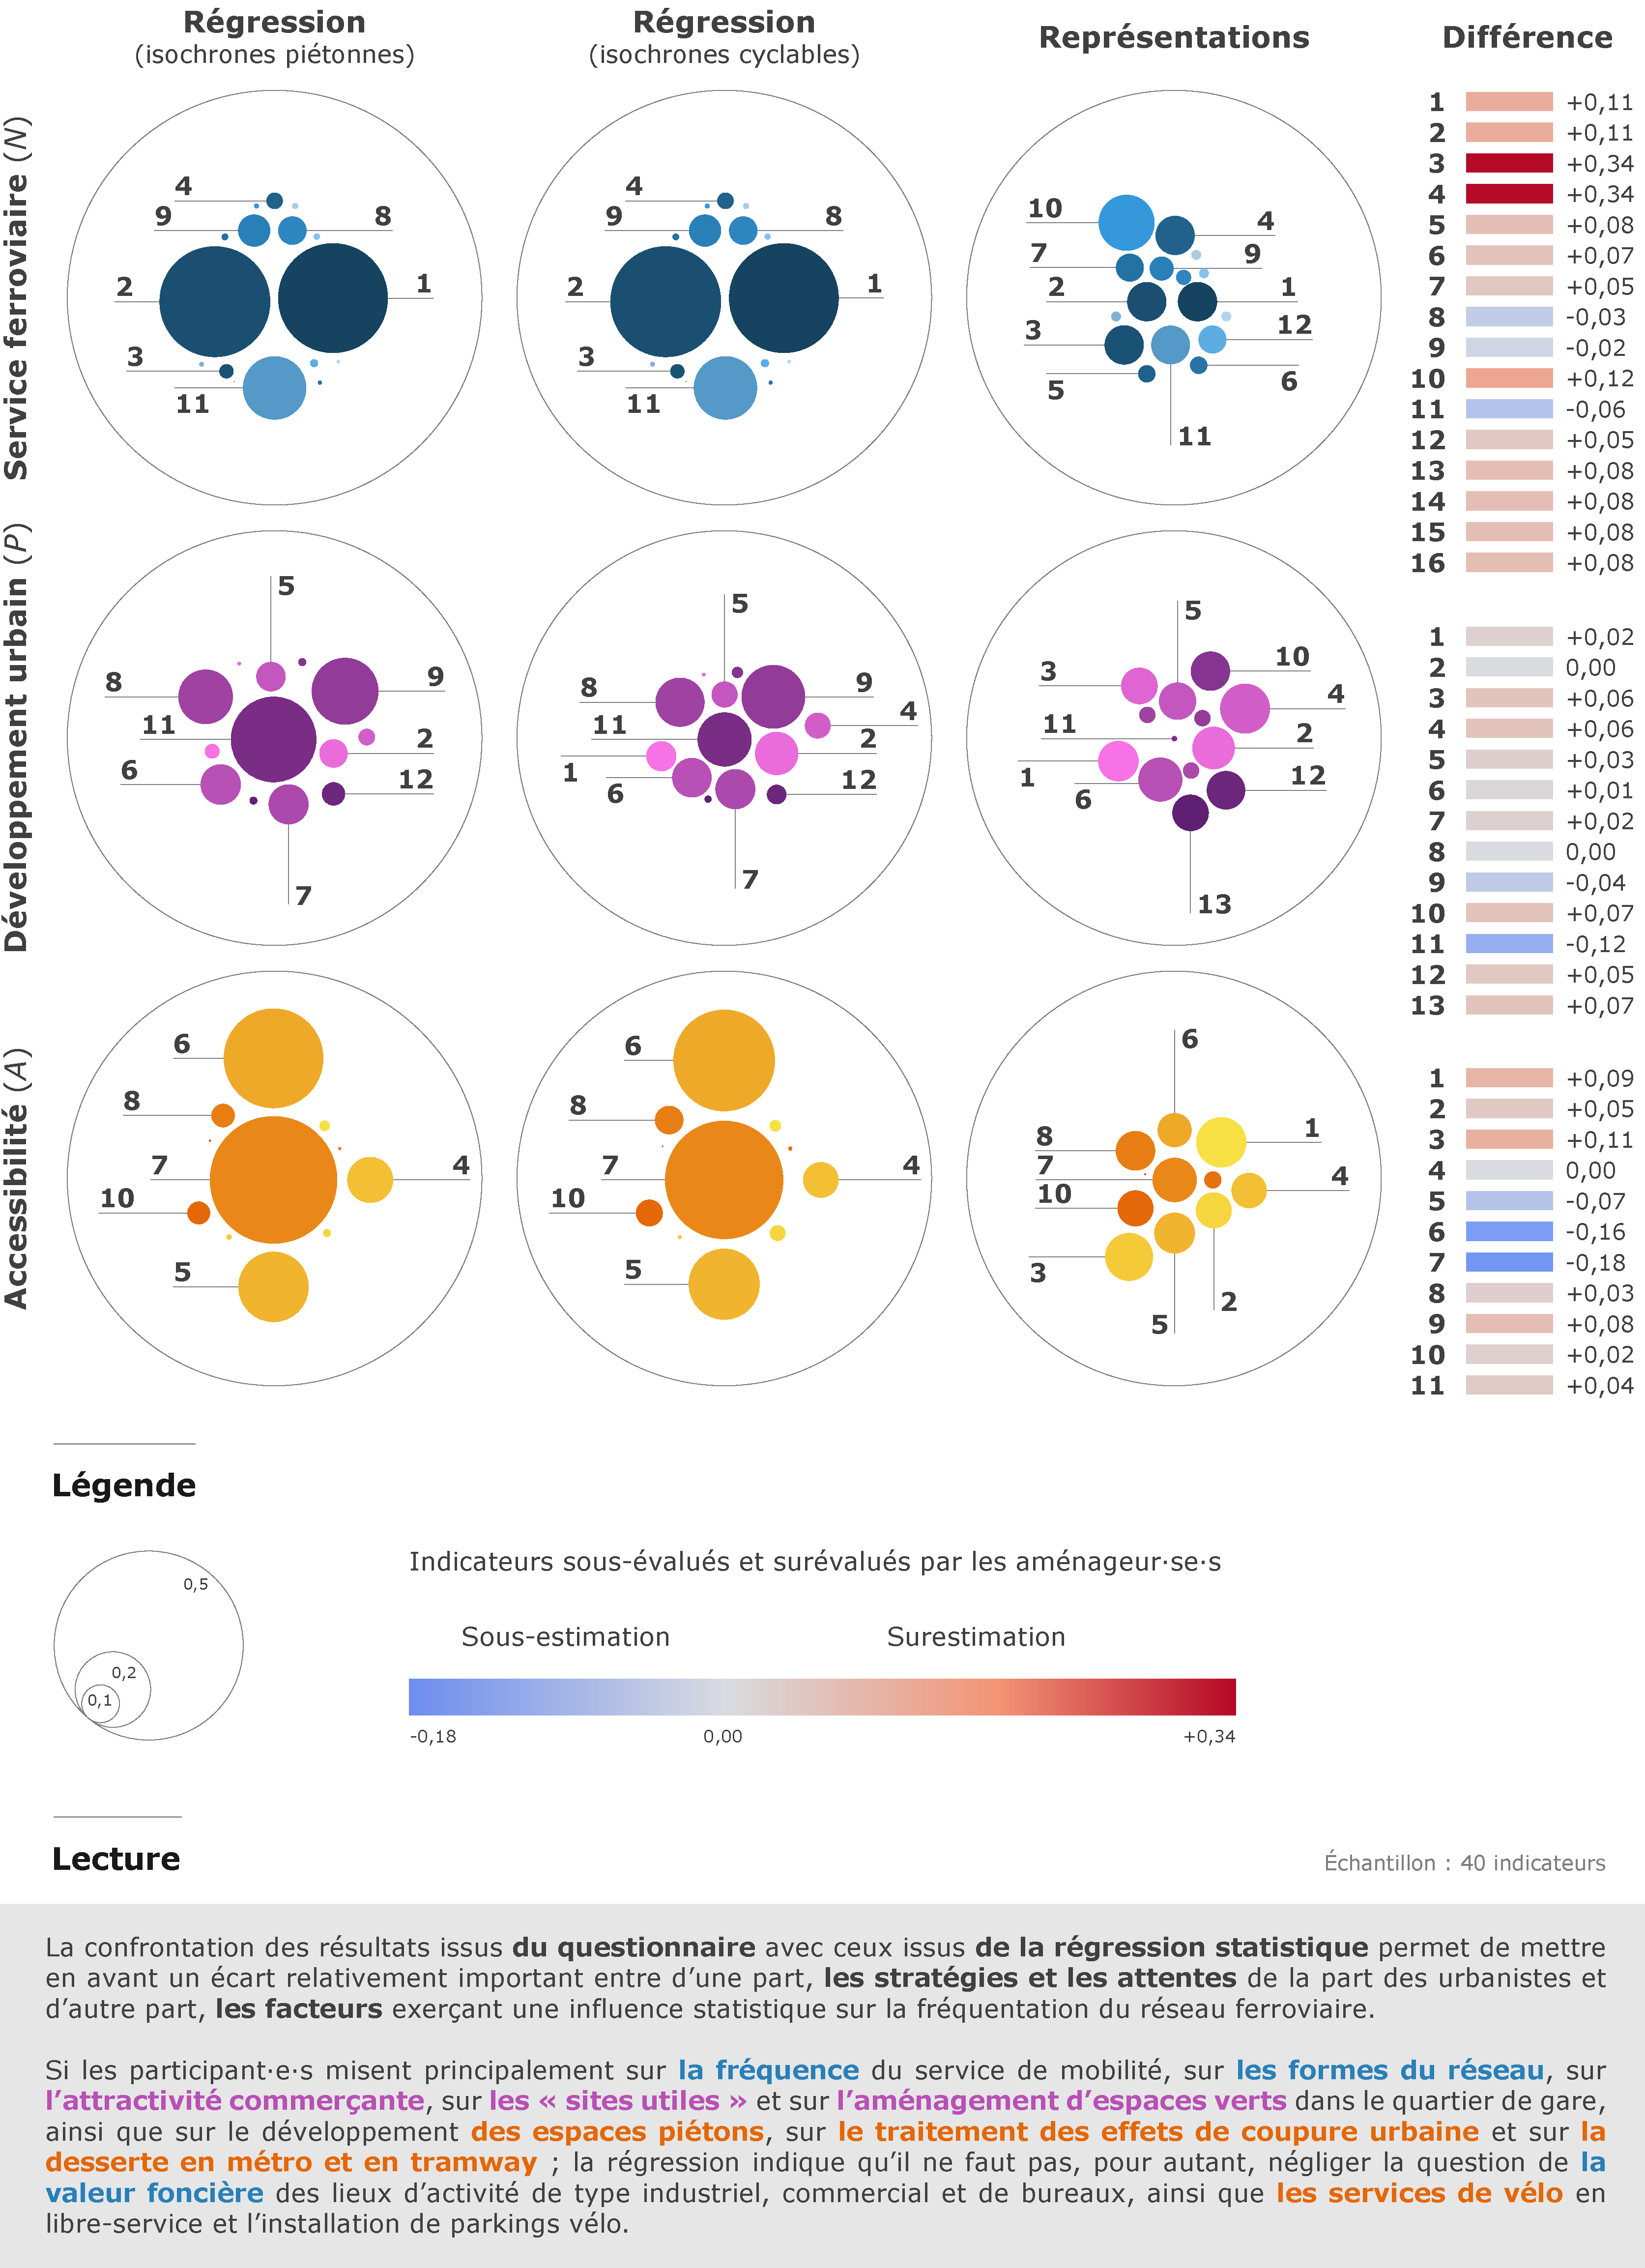
\includegraphics[width=1\columnwidth]{src/Figures/Chap-6/FR_NPART_Confrontation_Poids_Indicateurs.pdf}}
        \vspace{5pt}
        \begin{flushright}\scriptsize{
        Réalisation~: \textcolor{blue}{Dylan Moinse (2024)}
        \\
        Auteur·rice·s~: projet de recherche \acrshort{NPART}
        }\end{flushright}
    \end{figure}

    % Littérature node
Dans notre modèle, il apparaît que les acteur·rice·s de la fabrique urbaine ont tendance à surévaluer l'impact positif du service ferroviaire sur le \acrshort{TOD} et le \acrshort{M-TOD}, notamment en ce qui concerne la fréquence (\(N_{1}\), \(N_{2}\), \(N_{3}\) et \(N_{4}\)), l'amplitude horaire (\(N_{5}\) et \(N_{6}\)), la position nodale d'interconnexion (\(N_{10}\)) ainsi que l'accès direct aux métropoles (\(N_{13}\), \(N_{14}\), \(N_{15}\) et \(N_{16}\)). Ce constat est en accord avec les conclusions de \textcolor{blue}{\textcite[41]{lukman_development_2014}}\index{Lukman, Azhari|pagebf}\index{Singh, Yamini Jain|pagebf}, qui font remarquer que les urbanistes valorisent davantage les critères liés au système ferroviaire, lors d'un atelier de travail portant sur Arnhem et Nimègue, aux Pays-Bas. En particulier, \textcolor{blue}{\textcite[2~430]{kumar_developing_2020}}\index{Kumar,~P. Phani|pagebf}\index{Parida, Manoranjan|pagebf}\index{Sekhar, Ch. Ravi|pagebf} et \textcolor{blue}{\textcite[42]{lukman_development_2014}}\index{Lukman, Azhari|pagebf}\index{Singh, Yamini Jain|pagebf} identifient la fréquence des services comme le volet le plus apprécié par les planificateur·rice·s indien·ne·s et néerlandais·e·s, tandis que la position centrale des gares dans le réseau ressort comme un élément clé en Belgique \textcolor{blue}{\autocite[95]{caset_planning_2019}}\index{Caset, Freke|pagebf}, observations qui rejoignent les résultats de notre propre étude.

    % Littérature - environnement urbain
Concernant l'environnement bâti, souvent privilégié par les expert·e·s locaux·les dans la littérature \textcolor{blue}{\autocite[41]{lukman_development_2014}}\index{Lukman, Azhari|pagebf}\index{Singh, Yamini Jain|pagebf}, les participant·e·s ayant contribué à la calibration du \acrshort{NPART} semblent accorder moins d’importance à des aspects tels que la densité ou la diversité, ce qui peut paraître contre-intuitif. En revanche, iels surévaluent le rôle stratégique de la longueur du réseau piétonnier (\(A_{1}\)), le traitement des obstacles (\(A_{3}\)) et la limitation de la vitesse motorisée (\(A_{9}\)). Des points également relevés dans les travaux de \textcolor{blue}{\textcite[2~430]{kumar_developing_2020}}\index{Kumar,~P. Phani|pagebf}\index{Parida, Manoranjan|pagebf}\index{Sekhar, Ch. Ravi|pagebf} et dans le rapport de recherche publié par le \textcolor{blue}{\textcite[19]{transportation_research_board_transit-oriented_2005}}\index{Transportation Research Board@\textsl{Transportation Research Board}|pagebf}\index{National Academies of Sciences, Engineering, and Medicine@\textsl{National Academies of Sciences, Engineering, and Medicine}|pagebf}, où l'aménagement orienté vers la marche est jugé très utile par les aménageur·se·s interrogé·e·s. Néanmoins, les résultats de notre questionnaire croisés à notre modèle de régression statistique montrent que ces dernier·ère·s accordent moins de poids à l'offre de stationnement automobile ou à la connexion routière, de même qu'à la valeur foncière ou à la présence de bureaux et commerces, ce qui marque une divergence par rapport à la littérature scientifique \textcolor{blue}{\autocites[19]{transportation_research_board_transit-oriented_2005}[42]{lukman_development_2014}[95]{caset_planning_2019}}\index{Caset, Freke|pagebf}\index{Lukman, Azhari|pagebf}\index{Singh, Yamini Jain|pagebf}\index{Transportation Research Board@\textsl{Transportation Research Board}|pagebf}\index{National Academies of Sciences, Engineering, and Medicine@\textsl{National Academies of Sciences, Engineering, and Medicine}|pagebf}.%%Rédigé%%

    % Transition
L'étude de l'influence individuelle de chaque indicateur sur le \acrshort{TOD} à l'échelle piétonne et cyclable nous a permis de quantifier leurs effets sur l'attractivité des gares et de mettre en évidence les écarts existants entre les impacts réels et les représentations des concepteur·rice·s. Afin d'obtenir une vision plus précise du potentiel de développement par les systèmes de transport en commun de notre étude de cas régionale,  nous allons nous concentrer sur l'évaluation de l'accessibilité des gares et de leur environnement immédiat, en sondant les interactions entre les quatre dimensions du \acrshort{NPART}.%%Rédigé%%

    % 6.4.2.
    \needspace{1\baselineskip} % Réserve de l'espace
\subsection{Évaluation de l'accessibilité des nœuds et des quartiers de gare de la région
    \label{chap6:results-caracterisation-gares}
    }

    % Introduction
L'étape suivante consiste en la caractérisation des gares et de leurs quartiers environnants pour évaluer la situation d'\Guillemets{équilibre} des fonctions de chaque gare. Cette sous-section s’intéresse spécifiquement aux gares qualifiées de \Guillemets{dépendantes}, une catégorie qui prédomine dans le réseau étudié. En effet, ces gares se distinguent par des valeurs modérées ou faibles pour au moins deux des dimensions étudiées, traduisant une insuffisance dans la coordination entre la qualité du réseau ferroviaire, les dynamiques territoriales et les connexions locales. Cette situation est révélatrice de territoires où la demande de mobilité et l’attractivité des gares restent limitées. En nous appuyant sur des représentations graphiques tridimensionnelles et des indicateurs descriptifs pondérés, nous chercherons ainsi à approfondir la compréhension des facteurs qui limitent leur développement, tout en les situant par rapport à la catégorie complémentaire des gares \Guillemets{accessibles}. Par ailleurs, cette sous-section met en évidence des liens d’interdépendance significatifs entre les différentes dimensions du \acrshort{NPART}, renforçant ainsi l’hypothèse d’une nécessité de coordination étroite entre les réseaux de transport, le développement urbain et l’accessibilité locale.%%Rédigé%%

    % 6.4.2.1.
    \needspace{1\baselineskip} % Réserve de l'espace
\subsubsection*{Une région maillée de gares qualifiées de \Guillemets{dépendantes}
    \label{chap6:results-caracterisation-gares-dependance}
    }

    % Introduction
Cette première sous-section présente un exercice préliminaire d’étiquetage des gares et de leurs environs en fonction des valeurs obtenues pour chaque indicateur, tout en prenant en compte l'équilibre entre les dimensions analysées, à savoir la connectivité régionale, l'usage des sols et l'accessibilité locale. À cet effet, nous nous appuyons sur la notion de zone \Guillemets{accessible}, définie comme un état où les fonctions d'intensité de l'offre ferroviaire, d'intensité des activités et d'intensité des connexions se coordonnent de manière adéquate.%%Rédigé%%

    % Figure Diagrammes 3D - IEW
    \begin{figure}[h!]\vspace*{4pt}
        \caption{Diagrammes multidimensionnels positionnant les gares examinées, à l'échelle des isochrones piétonnes et cyclistes et au regard des dimensions du NPART.}
        \label{fig-chap6:diagramme-cubes}
        \centerline{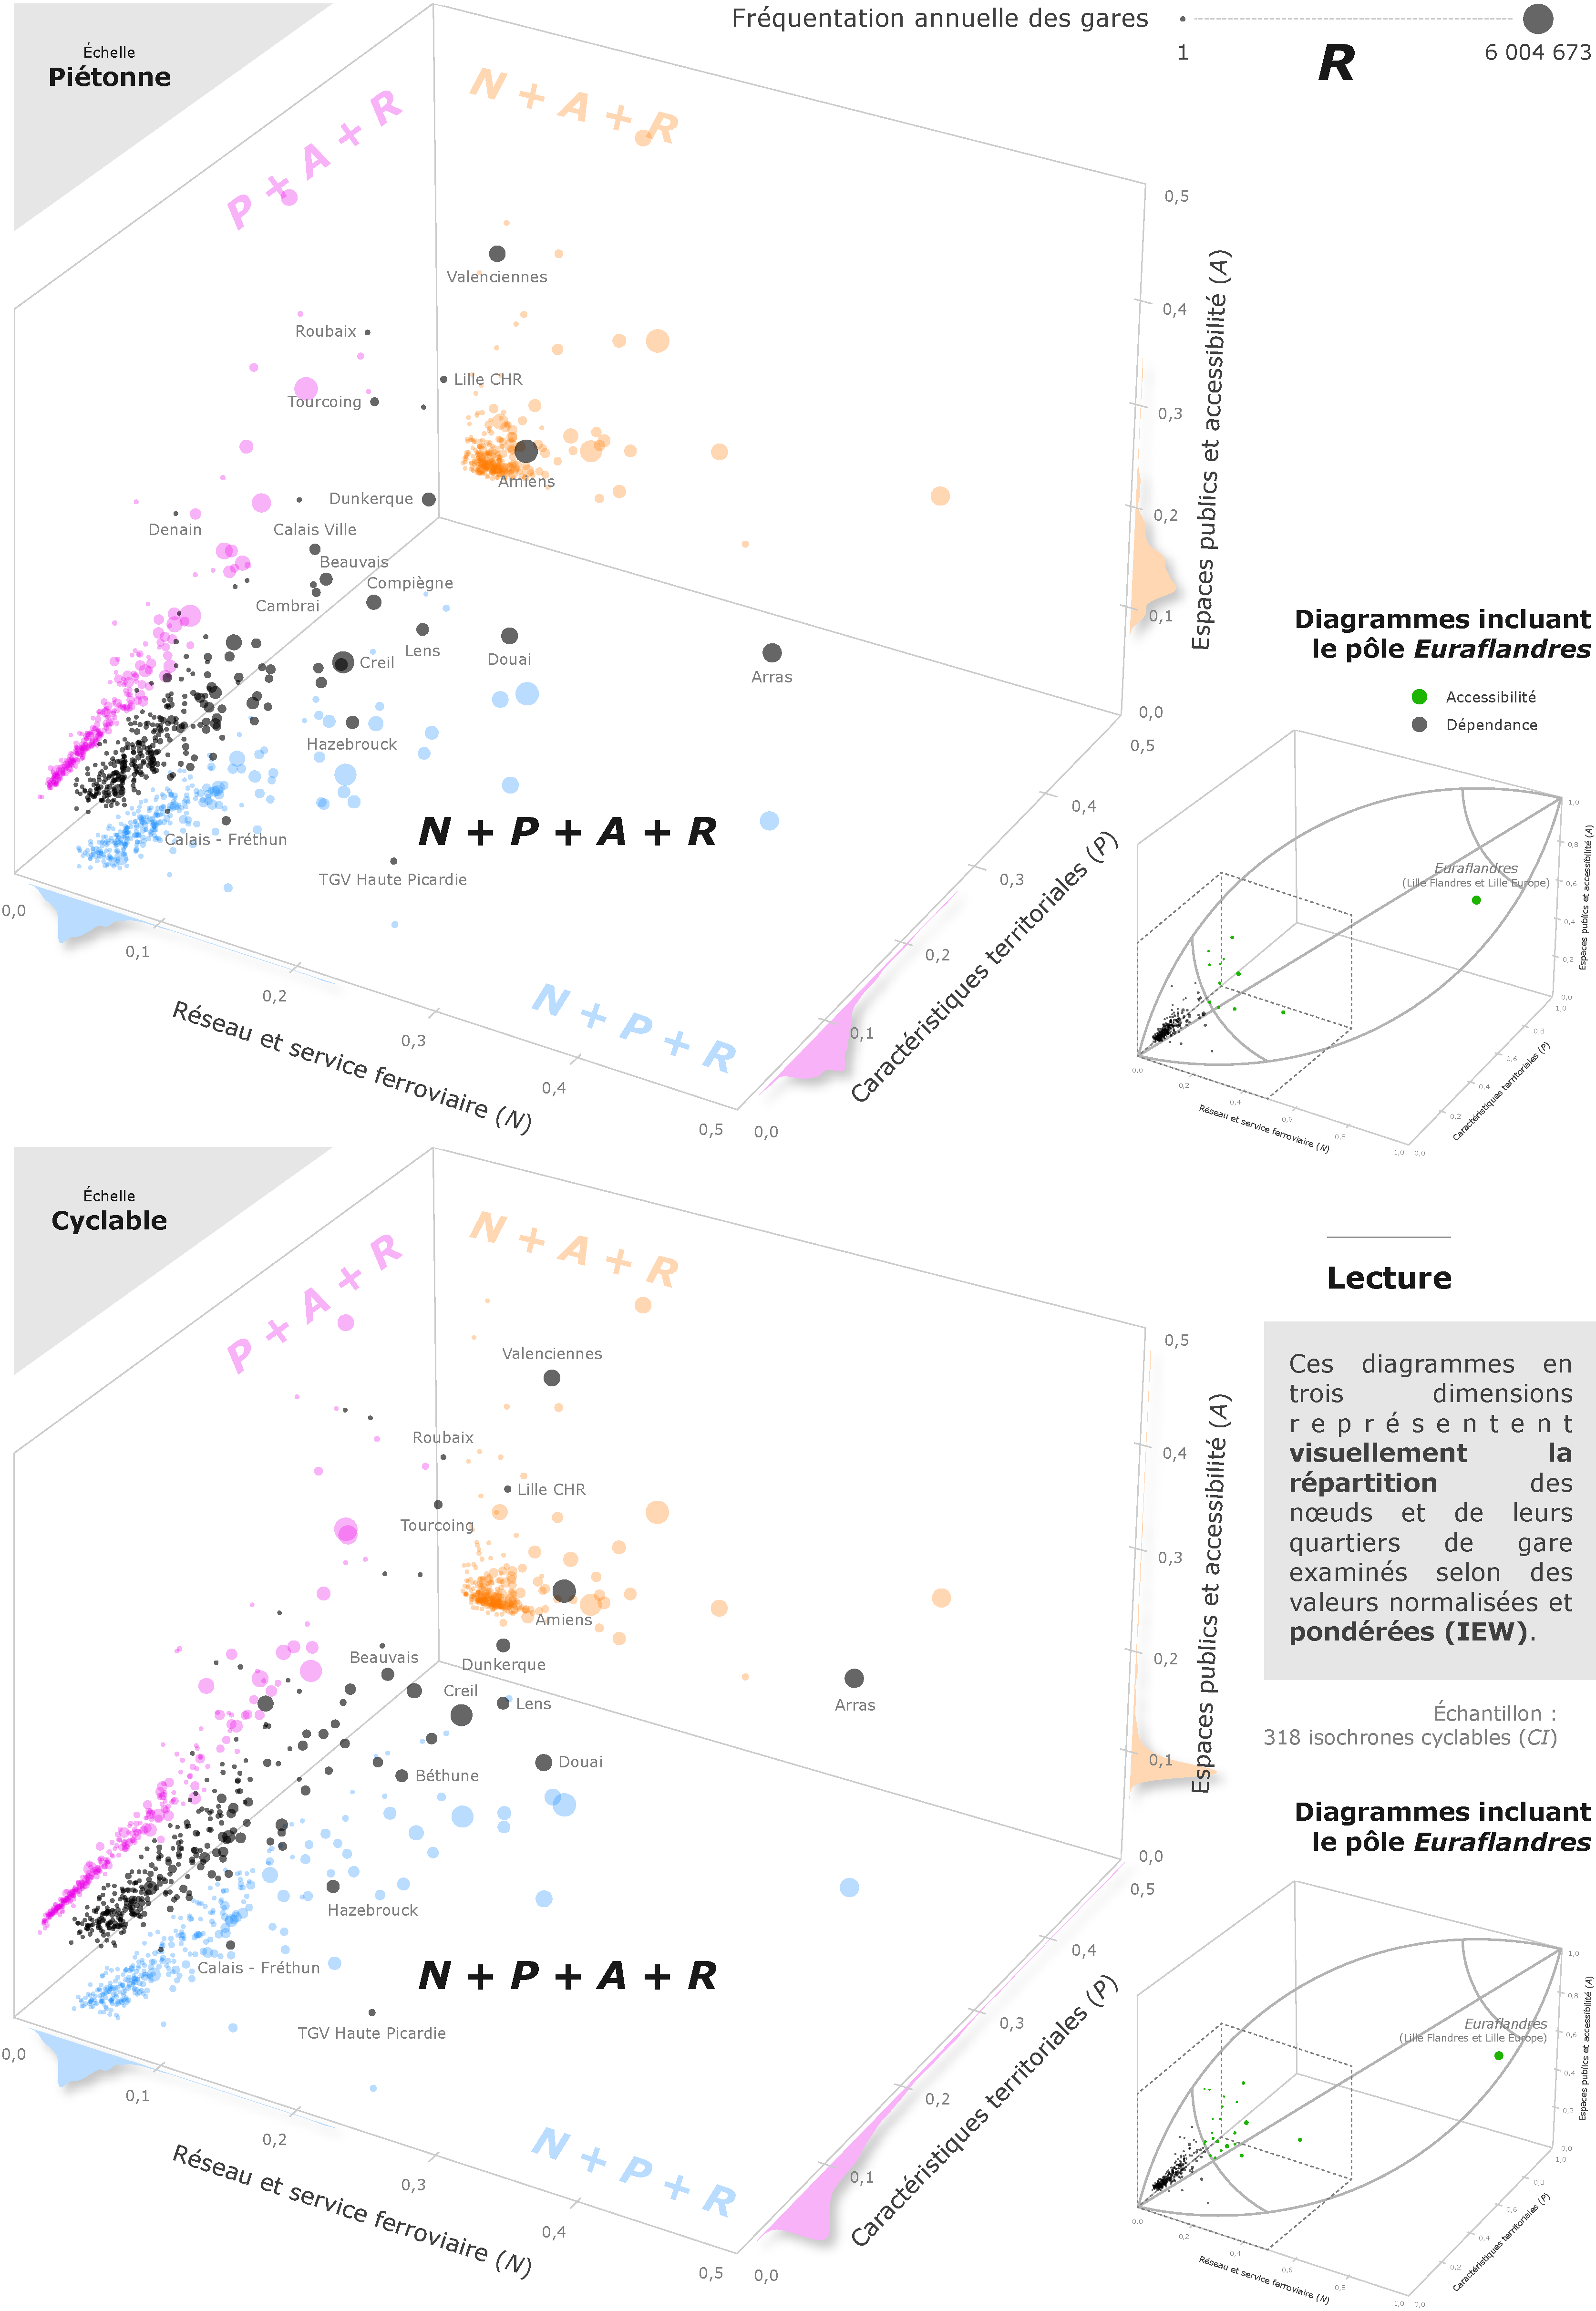
\includegraphics[width=1\columnwidth]{src/Figures/Chap-6/FR_NPART_Cubes.pdf}}
        \vspace{5pt}
        \begin{flushright}\scriptsize{
        Réalisation~: \textcolor{blue}{Dylan Moinse (2024)}
        \\
        Auteur·rice·s~: projet de recherche \acrshort{NPART}
        }\end{flushright}
    \end{figure}

    % Position des gares - dépendance
Pour l'ensemble des périmètres géographiques analysés, la majorité des gares étudiées se trouve dans la catégorie de \Guillemets{dépendance} (voir le \hyperref[fig-chap6:diagramme-cubes]{diagramme~\ref{fig-chap6:diagramme-cubes}}, page \pageref{fig-chap6:diagramme-cubes}). Cela est particulièrement vrai pour les deux types d'isochrones, où la proportion de gares considérées comme \Guillemets{dépendantes} atteint respectivement 96,23~\% pour l'échelle piétonne (\(PI\), 306 gares) et 92,77~\% pour l'échelle cyclable (\(CI\), 295 gares). Notons qu'aucun quartier de gare n'est en situation de profond \Guillemets{déséquilibre} en faveur de l'une des trois dimensions, ni en situation de \Guillemets{saturation}, nonobstant, le quartier de gare \textsl{Euraflandres} tend à s'en rapprocher.%%Rédigé%%

    % Position des gares - accessibilité (PI)
À l'échelle piétonne comme à l'échelle cyclable, seule une poignée de nœuds et de quartiers de gare peuvent être qualifiés d'\Guillemets{accessibles} ou d'\Guillemets{équilibrées}, pour reprendre la terminologie de \textcolor{blue}{Luca} \textcolor{blue}{\textcite[202]{bertolini_spatial_1999}}\index{Bertolini, Luca|pagebf}. Plus en détail, seules 12 gares entrent dans cette catégorie pour \(PI\), tandis que 23 le sont pour \(CI\). Il apparaît que les 12 gares \Guillemets{accessibles} pour \(PI\) le sont également pour \(CI\). Il s'agit des gares d'Amiens, d'Arras, de Compiègne, de Douai, de Dunkerque, d'\textsl{Euraflandres}, de Lens, de Lille CHR, de Pont de Bois, de Roubaix, de Tourcoing et de Valenciennes (voir le \hyperref[fig-chap6:diagramme-cubes]{diagramme~\ref{fig-chap6:diagramme-cubes}}, page~\pageref{fig-chap6:diagramme-cubes}). Comme nous pouvons le constater, les gares \Guillemets{accessibles} à l'échelle piétonne sont soit situées dans des communes centrales de la \acrfull{MEL}, soit dans le centre urbain de certaines sous-préfectures de la région.%%Rédigé%%

    % Position des gares - accessibilité (CI)
Il est donc pertinent de noter qu'en élargissant les quartiers de gare pour adapter leur taille à la portée de la mobilité individuelle légère, la région voit son nombre de lieux de connexion dits \Guillemets{accessibles} doubler. Les 11 gares qui rejoignent cette catégorie grâce à l'élargissement de l'aire d'influence des gares sont les suivantes~: Beauvais, Béthune, Boulogne-sur-Mer, Boulogne~–~Tintelleries, Calais Ville, Creil, Croix~–~Wasquehal, La Madeleine, Lille Porte de Douai, Saint-Quentin et Saint-Roch (voir le \hyperref[fig-chap6:diagramme-cubes]{diagramme~\ref{fig-chap6:diagramme-cubes}}, page~\pageref{fig-chap6:diagramme-cubes}). À ce titre, les gares qui deviennent \Guillemets{accessibles} à la suite de l'extension des isochrones se situent soit dans d'autres sous-préfectures de la région, soit à proximité des gares centrales des principales agglomérations.%%Rédigé%%

    % Littérature
L'identification d'une majorité substantielle de stations classées dans la catégorie des gares \Guillemets{dépendantes} n'est guère surprenante à l'échelle régionale, étant donné la diversité des territoires couverts et la variété de l'offre ferroviaire au sein du système étudié. Ce résultat contraste avec les observations de la littérature, \textcolor{blue}{Freke} \textcolor{blue}{\textcite[46]{caset_planning_2019}}\index{Caset, Freke|pagebf} mettant en évidence une prédominance de gares \Guillemets{déséquilibrées} en faveur de la qualité du service \acrfull{RER} et au détriment du \textsl{design}, dans la région bruxelloise. Le constat d'une proportion plus importante de points d'arrêt présentant un déséquilibre en défaveur du lieu est consolidé par \textcolor{blue}{\textcite[190]{kutty_assessment_2018}}\index{Kutty, Najeeba Ali Kunju Abdulla|pagebf} et \textcolor{blue}{\textcite[19]{monajem_evaluation_2015}}\index{Monajem, Saeed|pagebf}\index{Ekram Nosratian, Farzan|pagebf} qui signalent ce profil pour 20~\% des stations de métro à Téhéran, contre seulement 5~\% pour l'autre extrémité. Concernant les réseaux de \acrfull{BHNS} à Wates et à Téhéran, \textcolor{blue}{\textcite[15]{alfyan_node-place_2022}}\index{Alfyan, Muhammad Yusuf|pagebf}\index{Widyastuti, Dyah Titisari|pagebf} et \textcolor{blue}{\textcite[13]{pezeshknejad_evaluating_2020}}\index{Pezeshknejad, Parsa|pagebf}\index{Monajem, Saeed|pagebf}\index{Mozafari, Hamid|pagebf} identifient également une majorité d'arrêts en situation d'asymétrie, la première étude aux dépens du développement urbain et la seconde aux dépens des connexions, notamment en ce qui concerne la marchabilité. À l'inverse, le groupe principal de stations de métro modélisé par \textcolor{blue}{\textcite[12]{dou_integrating_2021}}\index{Dou, Mingxuan|pagebf}\index{Wang, Yandong|pagebf}\index{Dong, Shihai|pagebf} se situe en situation d'\Guillemets{équilibre} à Shanghai, tout comme \textcolor{blue}{\textcite[197]{reusser_classifying_2008}}\index{Reusser, Dominik~E.|pagebf}\index{Loukopoulos, Peter|pagebf}\index{Stauffacher, Michael|pagebf}\index{Scholz, Roland~W.|pagebf} dans le cadre du réseau ferroviaire suisse.%%Rédigé%%

    % Transition
Nous avons pu observer que le nombre de stations caractérisées par une bonne coordination entre les trois dimensions traitées double lorsque nous étendons le périmètre des quartiers de gare, validant l'hypothèse formulée par \textcolor{blue}{\textcite[518]{caset_measuring_2018}}\index{Caset, Freke|pagebf}\index{Vale, David~S.|pagebf}\index{Viana, Cláudia~M.|pagebf}, selon laquelle il existe un contraste marqué entre les aires de desserte ferroviaire évaluées à 800 ou 1~200 mètres et celles mesurées à 3~000 mètres. Ce résultat suggère que l'élargissement de l'échelle spatiale permet de mieux capturer les dynamiques locales et régionales qui influencent l'\Guillemets{équilibre} entre les fonctions de réseau, de territoire et de connexion. Plus généralement, nous constatons un creusement des écarts entre les gares et leurs environs les moins bien classés et ceux qui se situent en tête. Cet état des lieux soulève des questions sur les facteurs spécifiques qui placent ces stations dans de telles situations d'\Guillemets{accessibilité} ou de \Guillemets{dépendance}. Nous allons explorer les composantes déterminantes, en veillant à distinguer les portées piétonnes et cyclables.%%Rédigé%%

    % 6.4.2.2.
    \needspace{1\baselineskip} % Réserve de l'espace
\subsubsection*{Profil des gares \Guillemets{accessibles} et \Guillemets{dépendantes} sur la base des indicateurs descriptifs
    \label{chap6:results-profil-gares-dependance}
    }

    % Valeurs IEW statistiques
En moyenne, les valeurs correspondantes aux indicateurs pondérés (\acrshort{IEW}) pour les gares qualifiées d'\Guillemets{accessibles} (\(Acs\)) et de \Guillemets{dépendantes} (\(Dpt\)) se présente comme suit~:
\begin{customitemize}
    \item Concernant le nœud (\(N\)), la valeur moyenne pondérée atteint 0,013 pour \(N_{Acs}\) et 0,003 pour \(N_{Dpt}\), pour les échelles piétonnes et cyclables. L’écart en faveur de la première catégorie est ainsi 5,051 fois plus important pour l'échelle piétonne (\(PI\)), tandis qu'il se réduit à 3,646 pour l'échelle cyclable (\(CI\))~;
    \item En ce qui concerne le lieu (\(P\)), la valeur moyenne pondérée est de 0,024 pour \(P_{Acs}\) contre 0,006 pour \(P_{Dpt}\) à l’échelle piétonne. Cet écart en faveur des gares accessibles est de 4,395 pour \(PI\) et de 3,641 pour \(CI\)~; 
    \item Pour les connexions (\(A\)), la valeur moyenne pondérée s'élève à 0,025 pour \(A_{Acs}\) et à 0,007 pour \(A_{Dpt}\) à l’échelle piétonne. L’écart est ainsi de 3,518 pour \(PI\) en faveur des gares accessibles, et se réduit à 2,344 pour \(CI\)~;
    \item Concernant la fréquentation (\(RT\)), la valeur moyenne normalisée est de 0,151 pour \(RT_{Acs}\) contre 0,006 pour \(RT_{Dpt}\). L’écart est ainsi de 23,532 pour \(PI\) et de 18,345 pour \(CI\), en faveur des gares accessibles. \end{customitemize}%%Rédigé%%

    % Ecarts valeurs IEW - statistiques - au profit accessibles
En détail, en termes d’écart intra-variable, les trois indicateurs qui présentent la plus forte distinction entre les catégories pour l’échelle piétonne (\(PI\)) sont \(N_{1}\), avec un écart de 82,691, suivi de \(A_{7}\) avec 74,375, et \(N_{2}\) avec 73,921. Pour l’échelle cyclable (\(CI\)), les critères les plus discriminants restent \(N_{1}\), avec un écart de 66,146, \(N_{2}\) avec 58,96, et \(A_{6}\) avec 40,591. À l’inverse, certains indicateurs montrent un écart favorable aux gares qualifiées de \Guillemets{dépendantes}. Pour l’échelle piétonne (\(PI\)), les indicateurs concernés sont \(P_{13}\), avec un écart de 0,443, \(A_{10}\) avec 0,593, et \(P_{3}\) avec 0,916. Pour l’échelle cyclable (\(CI\)), on retrouve \(P_{13}\) avec un écart de 0,557 et \(A_{10}\) avec 0,622, tandis que \(P_{3}\) affiche un écart de 1,977.%%Rédigé%%

    % Résumé
En d’autres termes, les nœuds qualifiés d’\Guillemets{accessibles} présentent des valeurs relatives nettement plus élevées en ce qui concerne la fréquence des \acrshort{TGV}, et ce, indépendamment du jour de la semaine (\(N_{1}\) et \(N_{2}\)). De plus, pour le quartier de gare piéton, ils bénéficient d’une meilleure desserte en transport en commun urbain sur rail (\(A_{7}\)), tandis que pour le quartier de gare cyclable, ils affichent une meilleure liaison avec les services de \acrshort{VLS} (\(A_{6}\)). À l’inverse, les nœuds dits \Guillemets{dépendants} se caractérisent par un revenu médian des ménages plus élevé (\(P_{13}\)), une offre de stationnement automobile moins abondante dans l’\gls{espace public} (\(A_{10}\)), ainsi qu’une plus forte spécialisation résidentielle de leurs territoires (\(P_{3}\)), quelle que soit l’échelle spatiale considérée. Plus globalement, l’écart moyen des indicateurs est de 12,101 pour l’échelle piétonne (\(PI\)) et de 8,537 pour l’échelle cyclable (\(CI\)), ce qui suggère que le périmètre cyclable tend à tempérer quelque peu les disparités entre les gares \Guillemets{accessibles} et \Guillemets{dépendantes}.%%Rédigé%%

    % Transition
Nous avons pu, en tenant compte des différentes valeurs propres à chaque critère et dimension, situer chacune des gares étudiées dans les zones conceptuelles définies par \textcolor{blue}{Luca} \textcolor{blue}{\textcite[344]{bertolini_nodes_1996}}\index{Bertolini, Luca|pagebf}. Cette analyse par positionnement nous a permis, par ailleurs, de comparer les gares dites \Guillemets{accessibles} et \Guillemets{dépendantes} en fonction des échelles piétonnes et cyclables, offrant ainsi un regard novateur sur cette problématique. La dernière sous-section, dédiée à l’évaluation des nœuds de transport en commun, se concentre non plus sur les valeurs intrinsèques de chaque dimension, mais plutôt sur les relations qu'elles entretiennent entre elles.%%Rédigé%%

    % 6.4.2.3.
    \needspace{1\baselineskip} % Réserve de l'espace
\subsubsection*{Intensité et direction des relations entre les axes constitutifs du modèle
    \label{chap6:results-correlation-dimensions}
    }

    % Corrélation node - ridership (PI et CI)
Du point de vue des quatre dimensions structurant le \acrshort{NPART}, il ressort que certaines d'entre elles sont étroitement interconnectées. Par le calcul des matrices de corrélation de Pearson pour chaque paire de dimensions, nous avons tout d’abord mis en évidence une association positive particulièrement significative entre la dimension liée à la qualité du réseau ferroviaire (\(N\)) et celle relative à la demande de mobilité pour chaque gare (\(RT\)). Dans l’ensemble des données initiales, le coefficient de détermination \(R^2\) atteint ainsi 0,93 entre les dimensions concernant le nœud ferroviaire et la fréquentation des gares, indépendamment des périmètres géographiques considérés (\(PI\) et \(CI\)). Le test \(t\) associé\footnote{
    Le test \(t\) est une méthode statistique utilisée pour déterminer si une corrélation pourrait être due au hasard ou non, dans un contexte où il n'existe pas de véritable relation ou différence sous-jacente (hypothèse nulle). Précisons que la puissance de la statistique \(t\) est directement influencée par la taille de l'échantillon. C'est pour cette raison que le nombre d'observations doit toujours être prise en compte lors de l'interprétation de la significativité d'un test \(t\).
}, d’une valeur élevée de 43,60, démontre que cette corrélation est statistiquement très significative, la probabilité qu’elle soit due au hasard étant quasiment nulle. Il apparaît toutefois que cette relation linéaire forte entre les parties \textsl{Transit} et \textsl{Ridership per Time} n’est vérifiée que pour le sous-groupe des gares dites \Guillemets{accessibles}, avec un coefficient de corrélation de 0,96. En revanche, ce coefficient chute à une valeur modérée de 0,53 lorsque l’analyse se limite aux gares dites \Guillemets{dépendantes}. Cette observation découle d'un effet de segmentation, indiquant que la relation entre \(N\) et \(RT\) dépend de l’intensité et du degré d’articulation des valeurs propres à chaque dimension, caractérisant certaines gares comme des nœuds dits \Guillemets{accessibles}. Dans cette perspective, nous avons également exploré les relations existantes entre les autres dimensions.%%Rédigé%%

    % Corrélation node - design (PI et CI)
Une deuxième relation positive significative s'établit entre le nœud (\(N\)) et le \textit{design}, se matérialisant par l’aménagement des espaces publics et la connectivité locale (\(A\)). Le coefficient de corrélation de Pearson \(R^2\) atteint 0,75 pour le périmètre de gare piéton (\(PI\)) et 0,64 pour le périmètre cyclable (\(CI\)). De manière encore plus marquée que dans la première relation étudiée, nous observons un écart considérable entre les gares qualifiées d’\Guillemets{accessibles} et celles dites \Guillemets{dépendantes}. Les premières affichent des coefficients de détermination élevés (\(R^2\) à 0,77 pour \(PI\) et à 0,71 pour \(CI\)), tandis que pour les secondes, la corrélation est quasiment inexistante (\(R^2\) 0,21 pour \(PI\) et 0,02 pour \(CI\)).%%Rédigé%%

    % Corrélation place - design (PI et CI)
Une dernière relation linéaire positive significative se manifeste entre les dimensions liées au lieu (\(P\)) et au \textsl{design} (\(A\)), visibles sur le \hyperref[fig-chap6:diagramme-cubes]{diagramme~\ref{fig-chap6:diagramme-cubes}} (page \pageref{fig-chap6:diagramme-cubes}). Cette association demeure significative tant à l'échelle piétonne que cyclable, avec des coefficients de détermination respectifs de 0,80 (test \(t\) de 23,36) et de 0,77 (test \(t\) de 21,47). Ces résultats suggèrent que l’intensification des activités humaines au sein d’un territoire donné est à l'origine ou découle de liens d’interdépendance marqués avec la qualité des espaces publics. En veillant à toujours distinguer les gares qualifiées d’\Guillemets{accessibles} de celles qualifiées de \Guillemets{dépendantes}, et contrairement aux deux relations précédemment analysées, nous observons des variations mineures en ce qui concerne l’aire d’influence piétonne des gares, avec des coefficients de corrélation \(R^2\) de 0,77 pour les premières et de 0,72 pour les secondes. Cependant, l’écart est légèrement plus prononcé dans les quartiers de gare cyclables, où les gares dites \Guillemets{accessibles} présentent un coefficient de 0,80, contre 0,65 pour celles dites \Guillemets{dépendantes}.%%Rédigé%%

    % Littérature
L’analyse de régression statistique appliquée aux différentes dimensions étudiées révèle des interdépendances intéressantes, en particulier au sein du sous-échantillon de gares qualifiées d'\Guillemets{accessibles}. Ces mesures quantitatives rappellent les travaux sur le \textit{NPM étendu} développé par \textcolor{blue}{\textcite[289]{vale_extended_2018}}\index{Vale, David~S.|pagebf}\index{Viana, Cláudia~M.|pagebf}\index{Pereira, Mauro|pagebf}, qui, à l'instar de notre étude, mettent en évidence une corrélation positive significative entre les dimensions associées au \Guillemets{lieu} et au \Guillemets{\textsl{design}}. De leur côté, \textcolor{blue}{\textcite[10]{zhang_network_2019}}\index{Zhang, Yuerong|pagebf}\index{Marshall, Stephen|pagebf}\index{Manley, Ed.~J.|pagebf} ont également démontré le même lien important, avec un \(R^2\) s'élevant à 0,81. Mais aussi une relation pertinente entre le \Guillemets{nœud} et le \Guillemets{lieu} (\(R^2\) à 0,70), en confirmant par ailleurs le constat de \textcolor{blue}{\textcite[289]{vale_extended_2018}}\index{Vale, David~S.|pagebf}\index{Viana, Cláudia~M.|pagebf}\index{Pereira, Mauro|pagebf} d’une corrélation modérée entre le \Guillemets{nœud} et le \Guillemets{\textsl{design}}, à hauteur de 0,60. Ce dernier point diffère cependant de nos observations empiriques, qui semblent indiquer une forte corrélation entre \(N\) et \(A\), particulièrement à l’échelle piétonne pour les gares \Guillemets{accessibles} \textcolor{blue}{\autocite[79]{papa_accessibility_2015}}\index{Papa, Enrica|pagebf}\index{Bertolini, Luca|pagebf}. Enfin, la relation positive majeure entre \(N\) et \(RT\), notamment aux heures de pointe pour les gares \Guillemets{accessibles}, constitue un apport nouveau à la littérature sur le \acrshort{NPM}. Cela ne signifie cependant pas qu’une simple amélioration de l’infrastructure et du service ferroviaire suffirait à accroître la demande. La relation, de nature bilatérale, suggère de la même manière que la demande induit des améliorations de l’infrastructure, qui évolue pour répondre à cette demande croissante.%%Rédigé%%

    % Transition
En adoptant une première approche basée sur les zones d'\Guillemets{accessibilité} et de \Guillemets{dépendance}, nous avons pu qualifier et attribuer des valeurs spécifiques à chaque gare étudiée. Ce travail empirique a mis en relief une large majorité de gares et de quartiers de gare se positionnent du côté des nœuds et lieux \Guillemets{dépendants}, aucun point d’arrêt du réseau n’étant fondamentalement considéré comme \Guillemets{déséquilibré}. Par ailleurs, nous avons examiné les interactions entre les quatre dimensions structurant notre modèle \acrshort{NPART} au prisme de cette typologie. Il en ressort ainsi que les gares dites \Guillemets{accessibles} bénéficient d’effets de rétroaction entre ces quatre dimensions. Cependant, comme le soulignent \textcolor{blue}{\textcite[4]{zhang_make_2023}}\index{Zhang, Mengyuan|pagebf}\index{Lee, Jinwoo Brian|pagebf}, \Guillemets{\textsl{les cinq catégories du modèle original node-place n'englobent pas toutes les typologies possibles des quartiers de gare et des formes de développement urbain orienté vers les transports en commun}}\footnote{
    \Guillemets{\textsl{In addition, the original node-place model’s five types of categories do not encompass all possible typologies of station areas and TODs}} \textcolor{blue}{\autocite[4]{zhang_make_2023}}\index{Zhang, Mengyuan|pagebf}\index{Lee, Jinwoo Brian|pagebf}.
}. Bien qu'à partir de ces diverses valeurs nous ayons pu classifier les stations et leur environnement immédiat à l’échelle piétonne et cyclable, notre analyse se poursuit en affinant la classification des gares étudiées afin d'affiner cette typologie.%%Rédigé%%

    % 6.4.3.
    \needspace{1\baselineskip} % Réserve de l'espace
\subsection{Classification des points nodaux et de leurs zones accessibles à pied, à vélo et en micro-mobilité
    \label{chap6:results-classification-gares}
    }

    % Introduction
Si les gares et leurs environnements immédiats occupent une place centrale dans l’interconnexion des espaces à l’échelle régionale, toutes ne bénéficient pas d’un positionnement équivalent en termes de connectivité, de densité des activités humaines ou de qualité des aménagements. Dans ce cadre, la finalité de cette modélisation est de proposer une classification des gares et de leurs zones d’influence en fonction de leurs performances respectives. Il s’agit de dépasser une catégorisation binaire (\Guillemets{accessibles} ou \Guillemets{dépendantes}) pour élaborer une typologie plus nuancée des points nodaux et des territoires environnants, en tenant compte de leur capacité à répondre aux principes du \acrshort{TOD} et du \acrshort{M-TOD}. L’ambition ne se limite pas à une classification statistique~; elle vise également, dans une logique de convergence entre science des données et géographie, à contextualiser et à donner du sens à ces catégories. Comme indiqué précédemment, et compte tenu de la diversité des typologies obtenues selon les paramètres définis, la section consacrée à l’exposé des résultats se concentre sur une étude de cas. Cette dernière s’appuie sur un portrait spécifique~: une analyse fondée sur des indicateurs pondérés par la méthode statistique \acrshort{IEW} durant les heures de pointe matinales (\(RT_{2}\)), sur la méthode de clustérisation des k-moyennes et appliquée à la fois à l’échelle piétonne (\(PI\)) et cyclable (\(CI\)).%%Rédigé%%

    % 6.4.3.1.
    \needspace{1\baselineskip} % Réserve de l'espace
\subsubsection*{Classification du réseau ferroviaire régional et des territoires environnants
    \label{chap6:results-classification-gares-classes}
    }

    % Classes
Comme détaillé dans la \hyperref[chap6:methodologie-statistiques-nombre-clusters]{sous-section méthodologique au sujet de la détermination du nombre optimal de classes~\ref{chap6:methodologie-statistiques-nombre-clusters}} (page~\pageref{chap6:methodologie-statistiques-nombre-clusters}), l’application de la méthode employée a permis de dégager trois classes de stations. Dans le cadre de notre étude de cas, la classification des 318 gares et quartiers de gare conduit, tant pour l’échelle piétonne (\(PI\)) que cyclable (\(CI\)), à l’identification d’une première classe (\(C1\)) regroupant les gares les plus attractives, dont le cadre urbain est élaboré et bien aménagé~; une deuxième classe (\(C2\)), comprenant les gares bénéficiant d'une infrastructure développée et situées dans des territoires dynamiques, mais faiblement orientés vers le pôle de mobilité~; et une dernière classe (\(C3\)), constituée des gares moins bien desservies et implantées dans des territoires où l’automobile prédomine.%%Rédigé%%

    % Figure changement de classe
    \begin{figure}[h!]\vspace*{4pt}
        \caption{Vers un doublement du nombre de gares comprises dans la première classe.}
        \label{fig-chap6:cubes-classification}
        \centerline{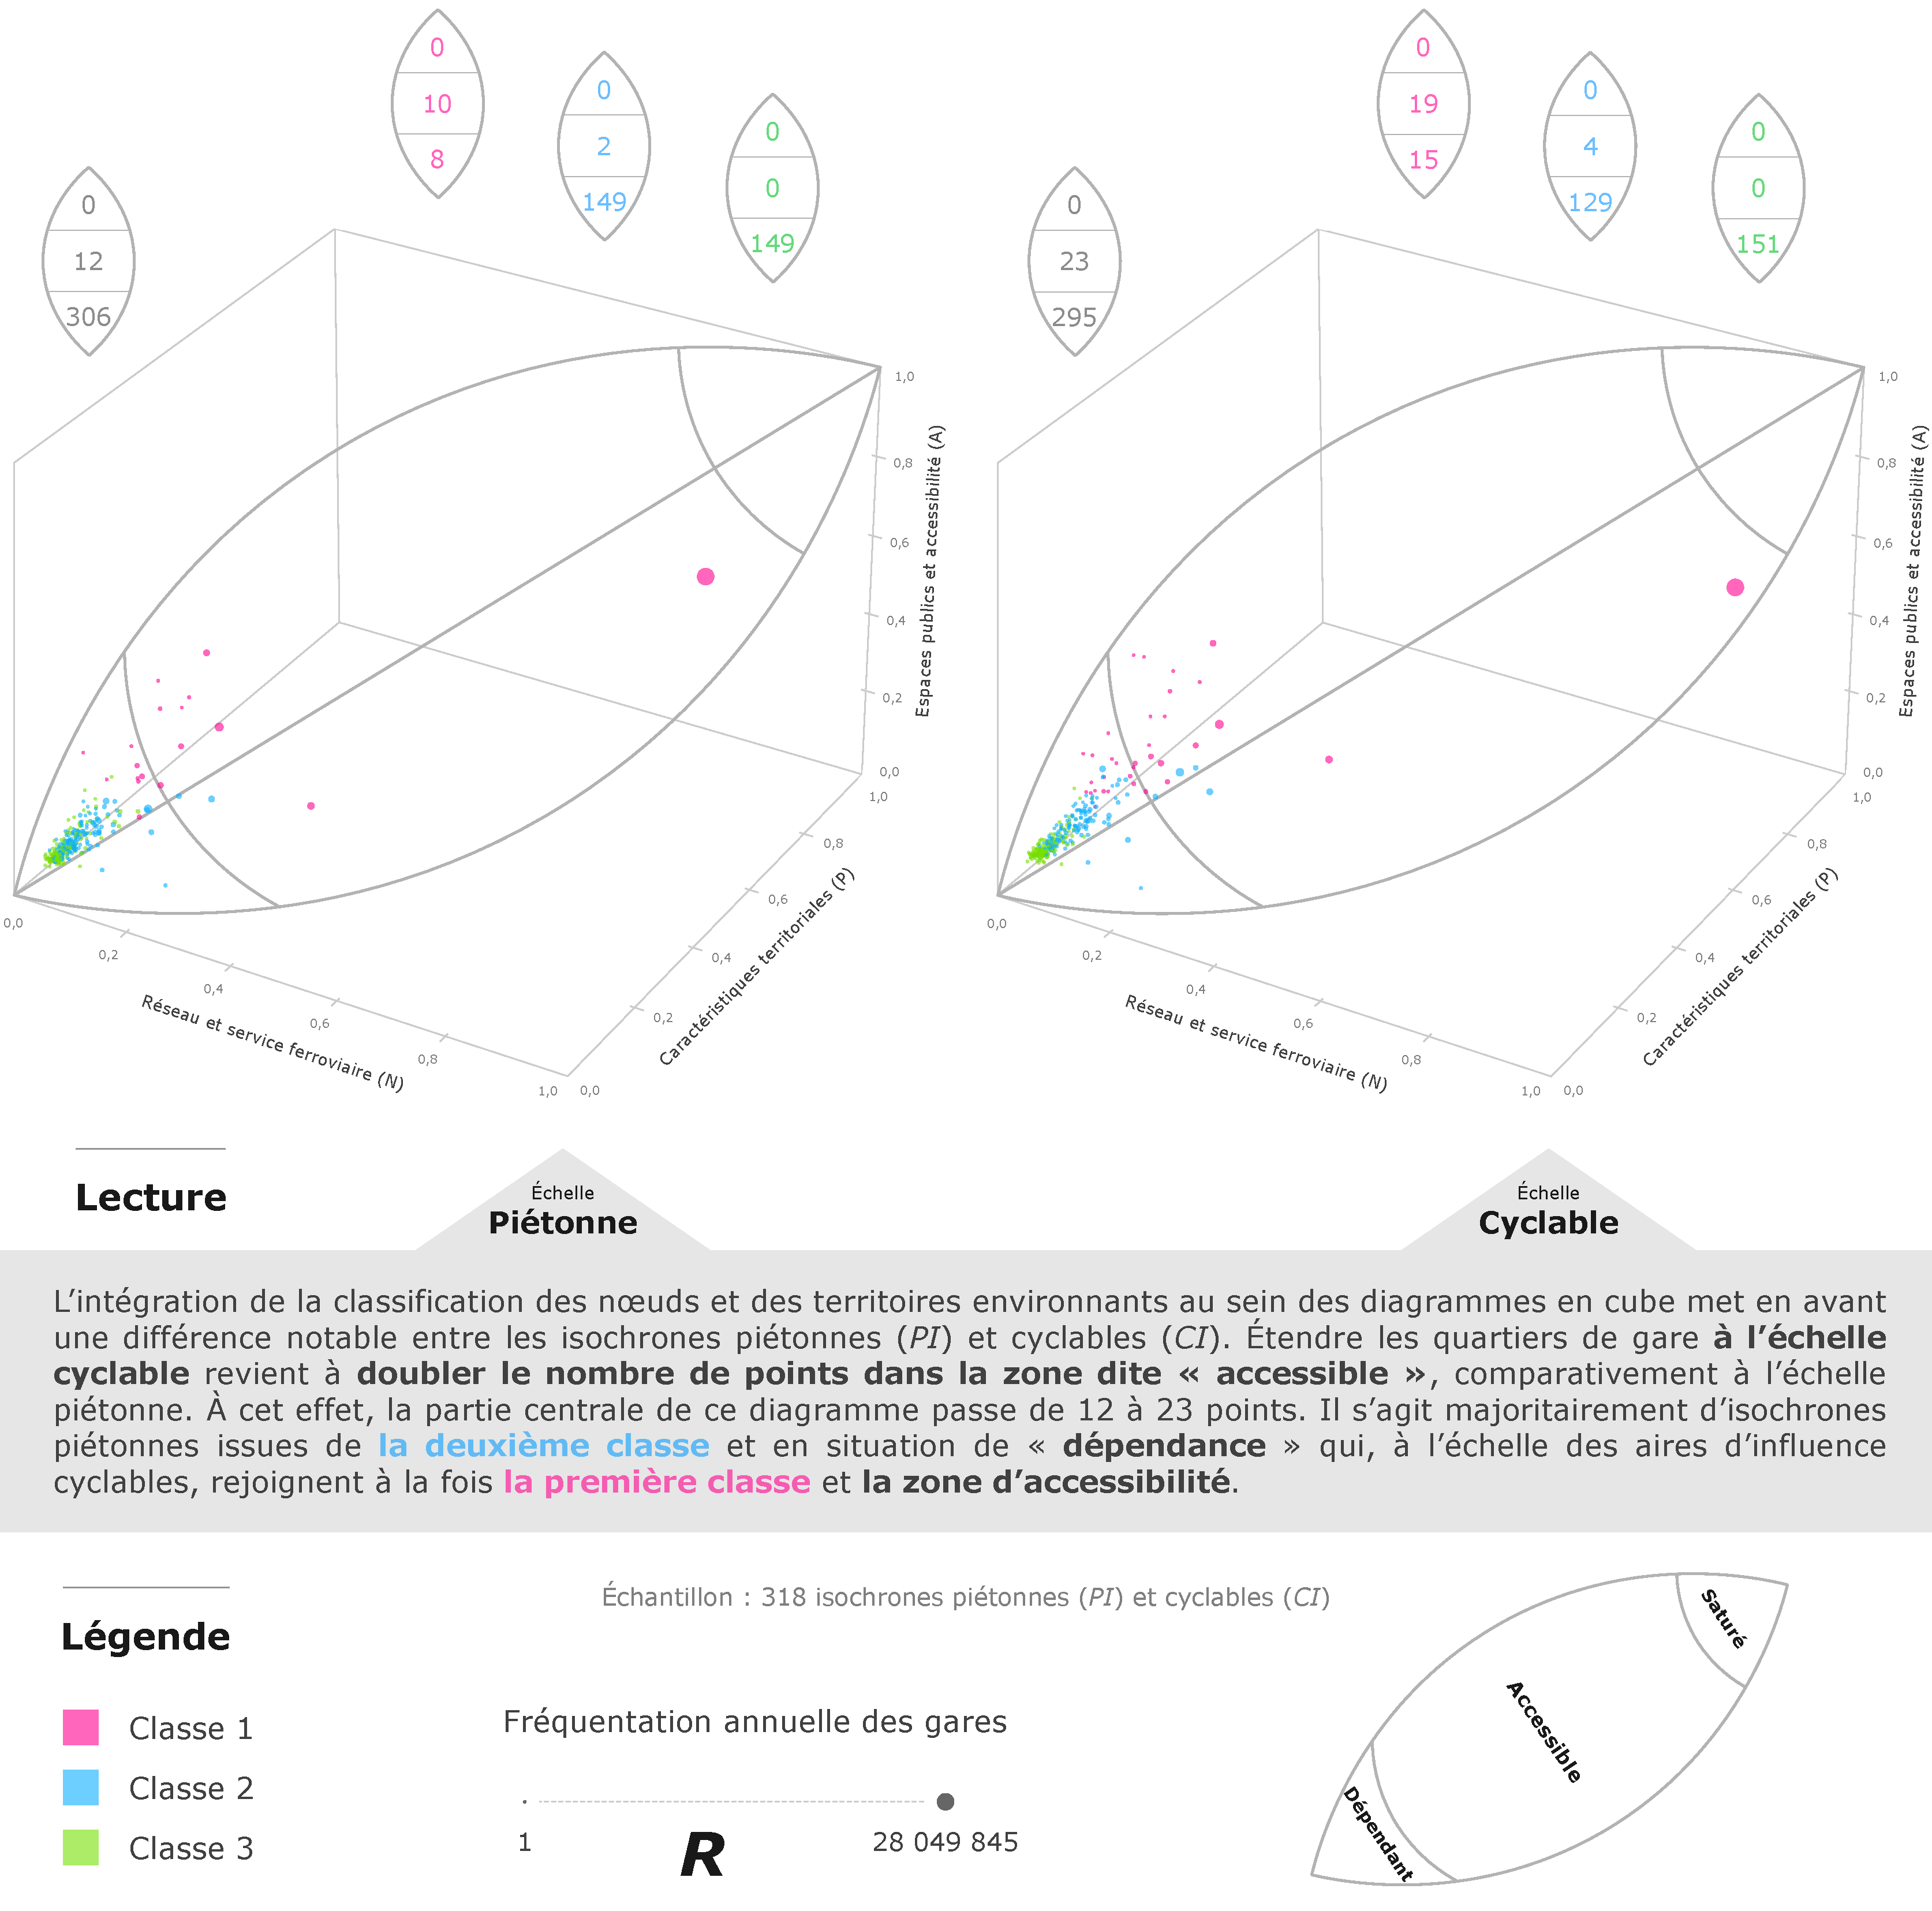
\includegraphics[width=1\columnwidth]{src/Figures/Chap-6/FR_NPART_Cubes_Classification.pdf}}
        \vspace{5pt}
        \begin{flushright}\scriptsize{
        Réalisation~: \textcolor{blue}{Dylan Moinse (2024)}
        \\
        Auteur·rice·s~: projet de recherche \acrshort{NPART}
        }\end{flushright}
    \end{figure}

    % Classes PI vs CI
À l'instar de la proportion prédominante de gares qualifiées de \Guillemets{dépendantes} dans la région, la quasi-totalité de celles-ci se retrouve également dans les deux dernières classes. Pour \(PI\), seules 5,66~\% des gares sont assignées à la classe \(C1\) (18 gares), tandis que 47,48~\% se situent dans \(C2\) (151 gares) et 46,86~\% dans \(C3\) (149 gares). Néanmoins, du côté de \(CI\), l’effectif de \(C1\) double (10,69~\%, 34 gares), principalement aux dépens de \(C2\) (41,82~\%, 133 gares), tandis que \(C3\) garde une part semblable (47,48~\%, soit 151 gares). Ainsi, l’extension des quartiers de gare au moyen de la mobilité individuelle légère permet à divers points d'arrêt de progresser de la classe \(C2\) à \(C1\). Il est intéressant de souligner que l’élargissement des quartiers de gare permet certes de doubler le nombre de gares dans \(C1\). Cependant, parmi les 16 nouvelles gares ainsi intégrées à cette catégorie, 7 d'entre elles restent qualifiées de \Guillemets{dépendantes} (voir l’\hyperref[fig-chap6:cubes-classification]{illustration~\ref{fig-chap6:cubes-classification}}, page~\pageref{fig-chap6:cubes-classification}).%%Rédigé%%

    % Carte Classification gares PI
    \begin{carte}[h!]\vspace*{4pt}
        \caption{Répartition des gares du réseau ferroviaire régional parmi les trois classes de quartiers de gare accessibles à pied (\(PI\)).}
        \label{fig-chap6:classification-gares-pieton}
        \centerline{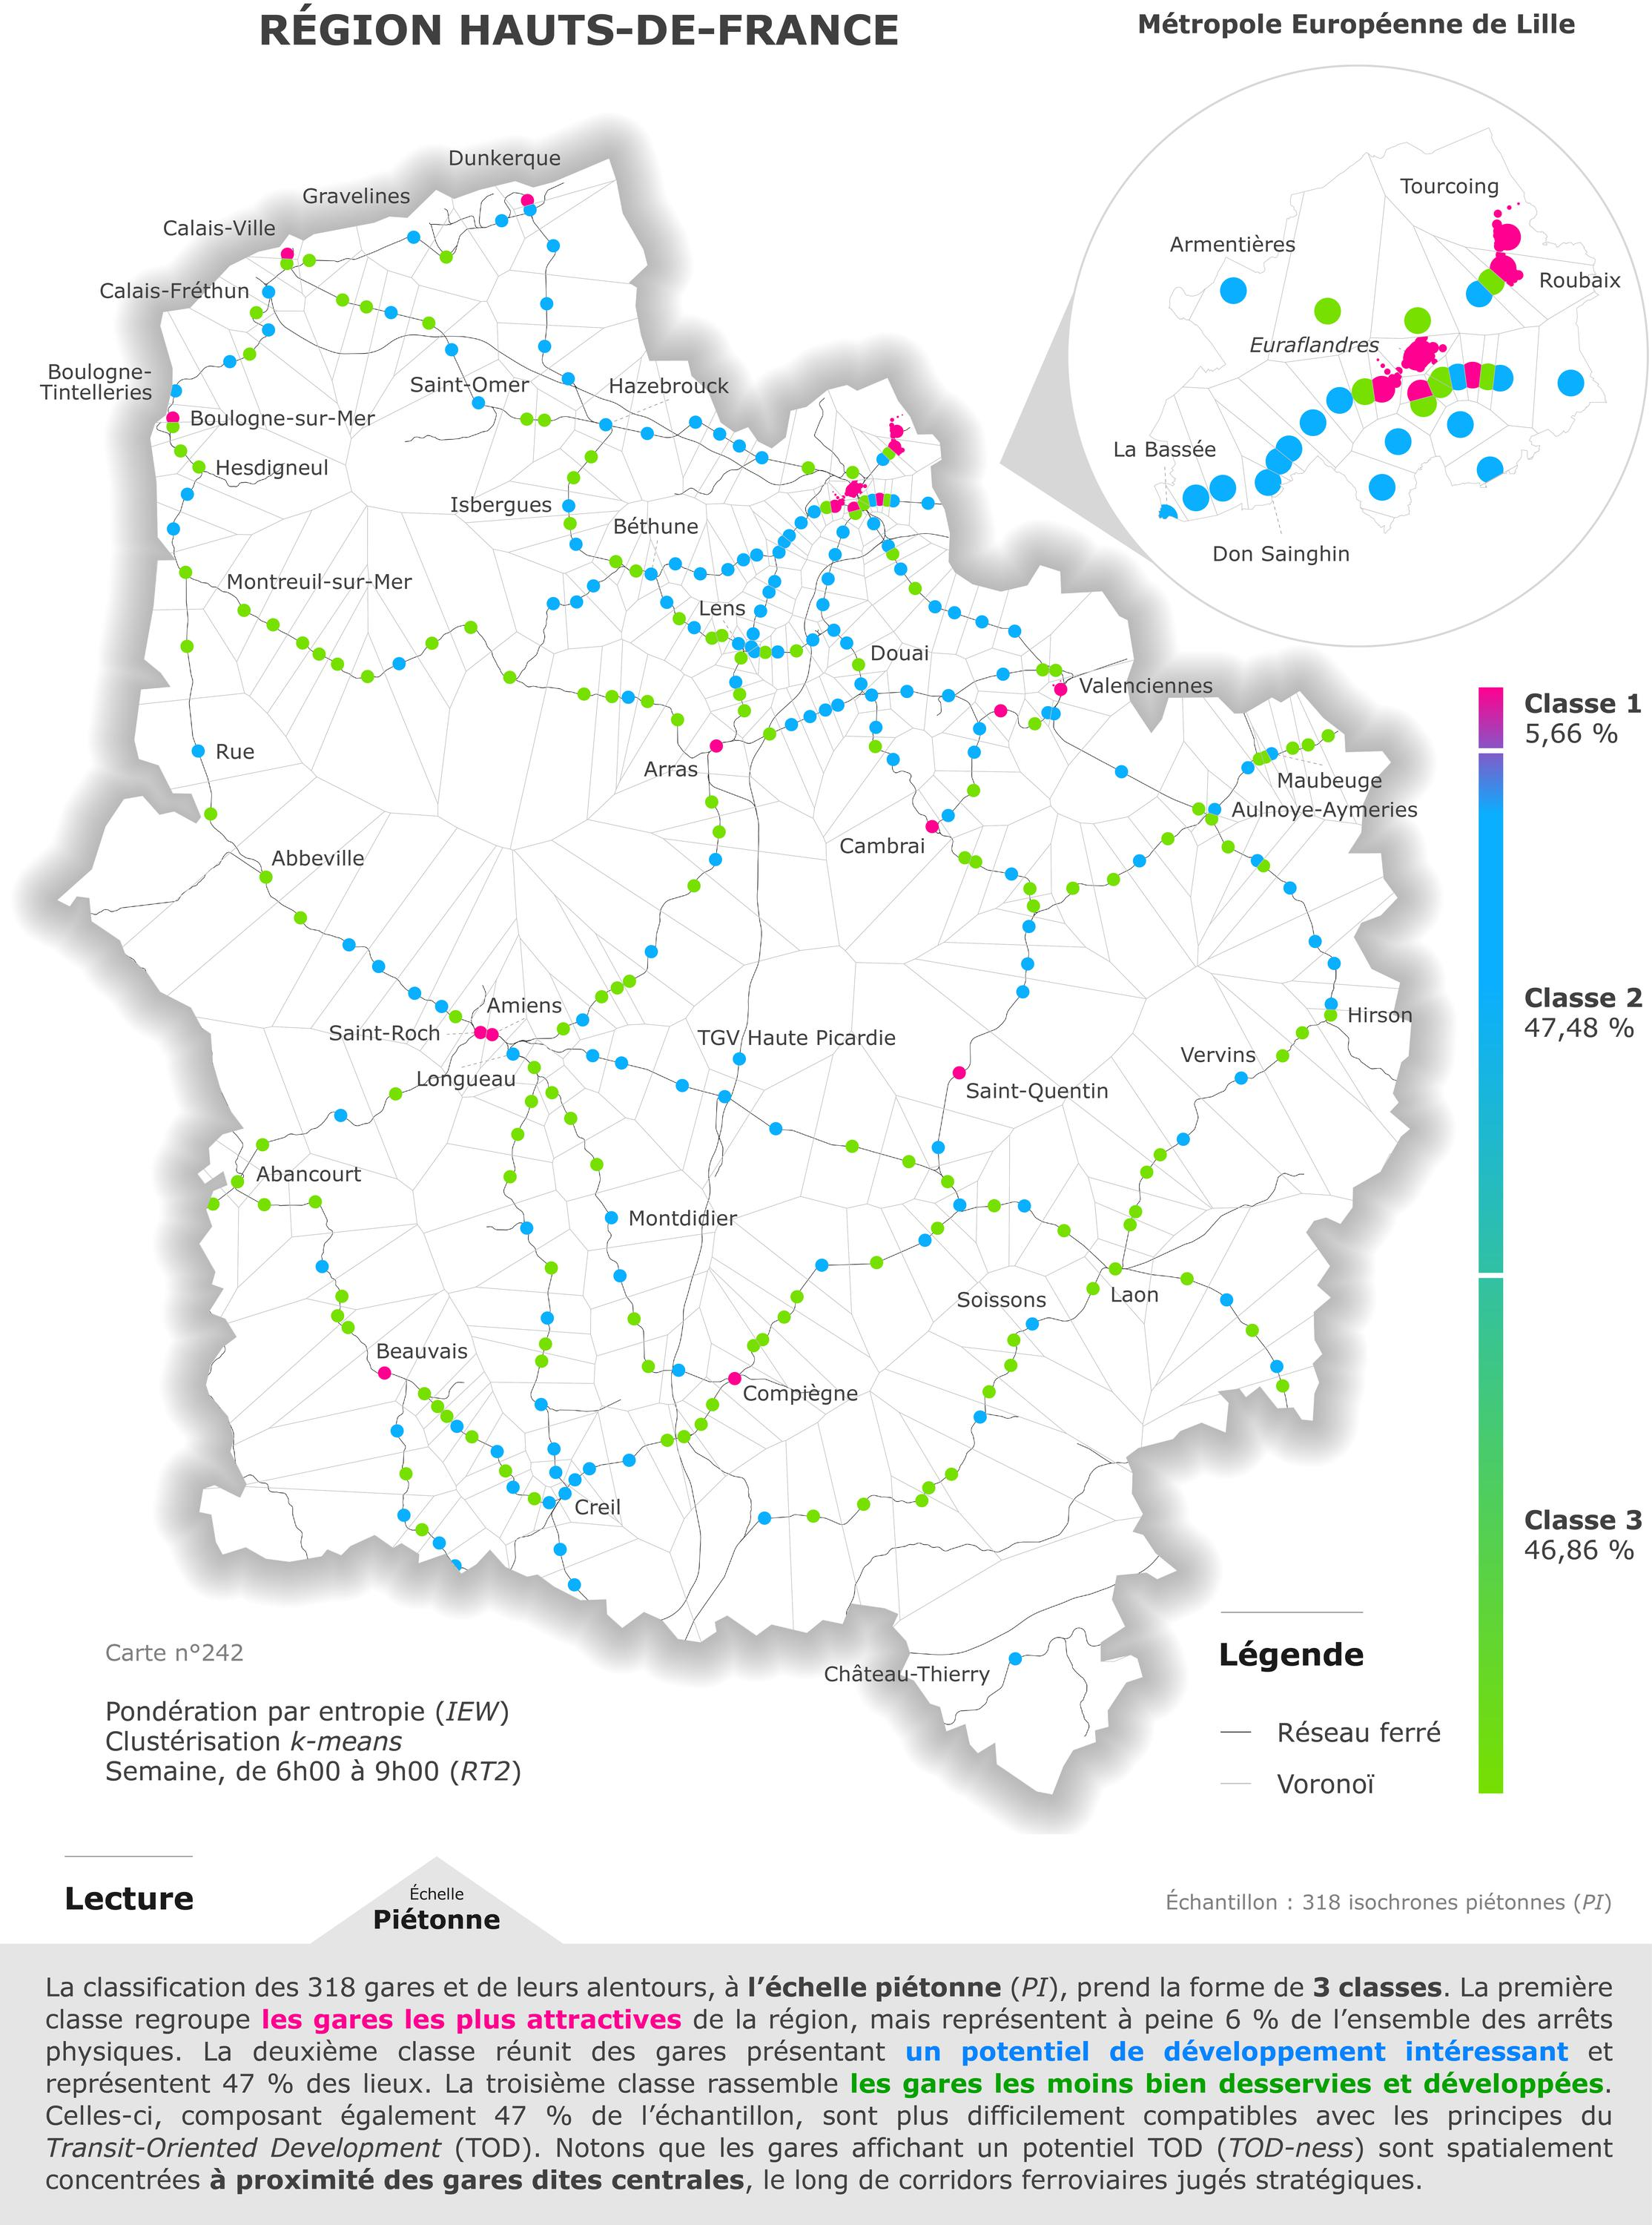
\includegraphics[width=1\columnwidth]{src/Figures/Chap-6/FR_NPART_Carte_Classification_PI.jpg}}
        \vspace{5pt}
        \begin{flushright}\scriptsize{
        Réalisation~: \textcolor{blue}{Dylan Moinse (2024)}
        \\
        Auteur·rice·s~: projet de recherche \acrshort{NPART}
        }\end{flushright}
    \end{carte}

    % Carte Classification gares CI
    \begin{carte}[h!]\vspace*{4pt}
        \caption{Répartition des gares du réseau ferroviaire régional parmi les trois classes de quartiers de gare accessibles en mobilité individuelle légère (\(CI\)).}
        \label{fig-chap6:classification-gares-cyclable}
        \centerline{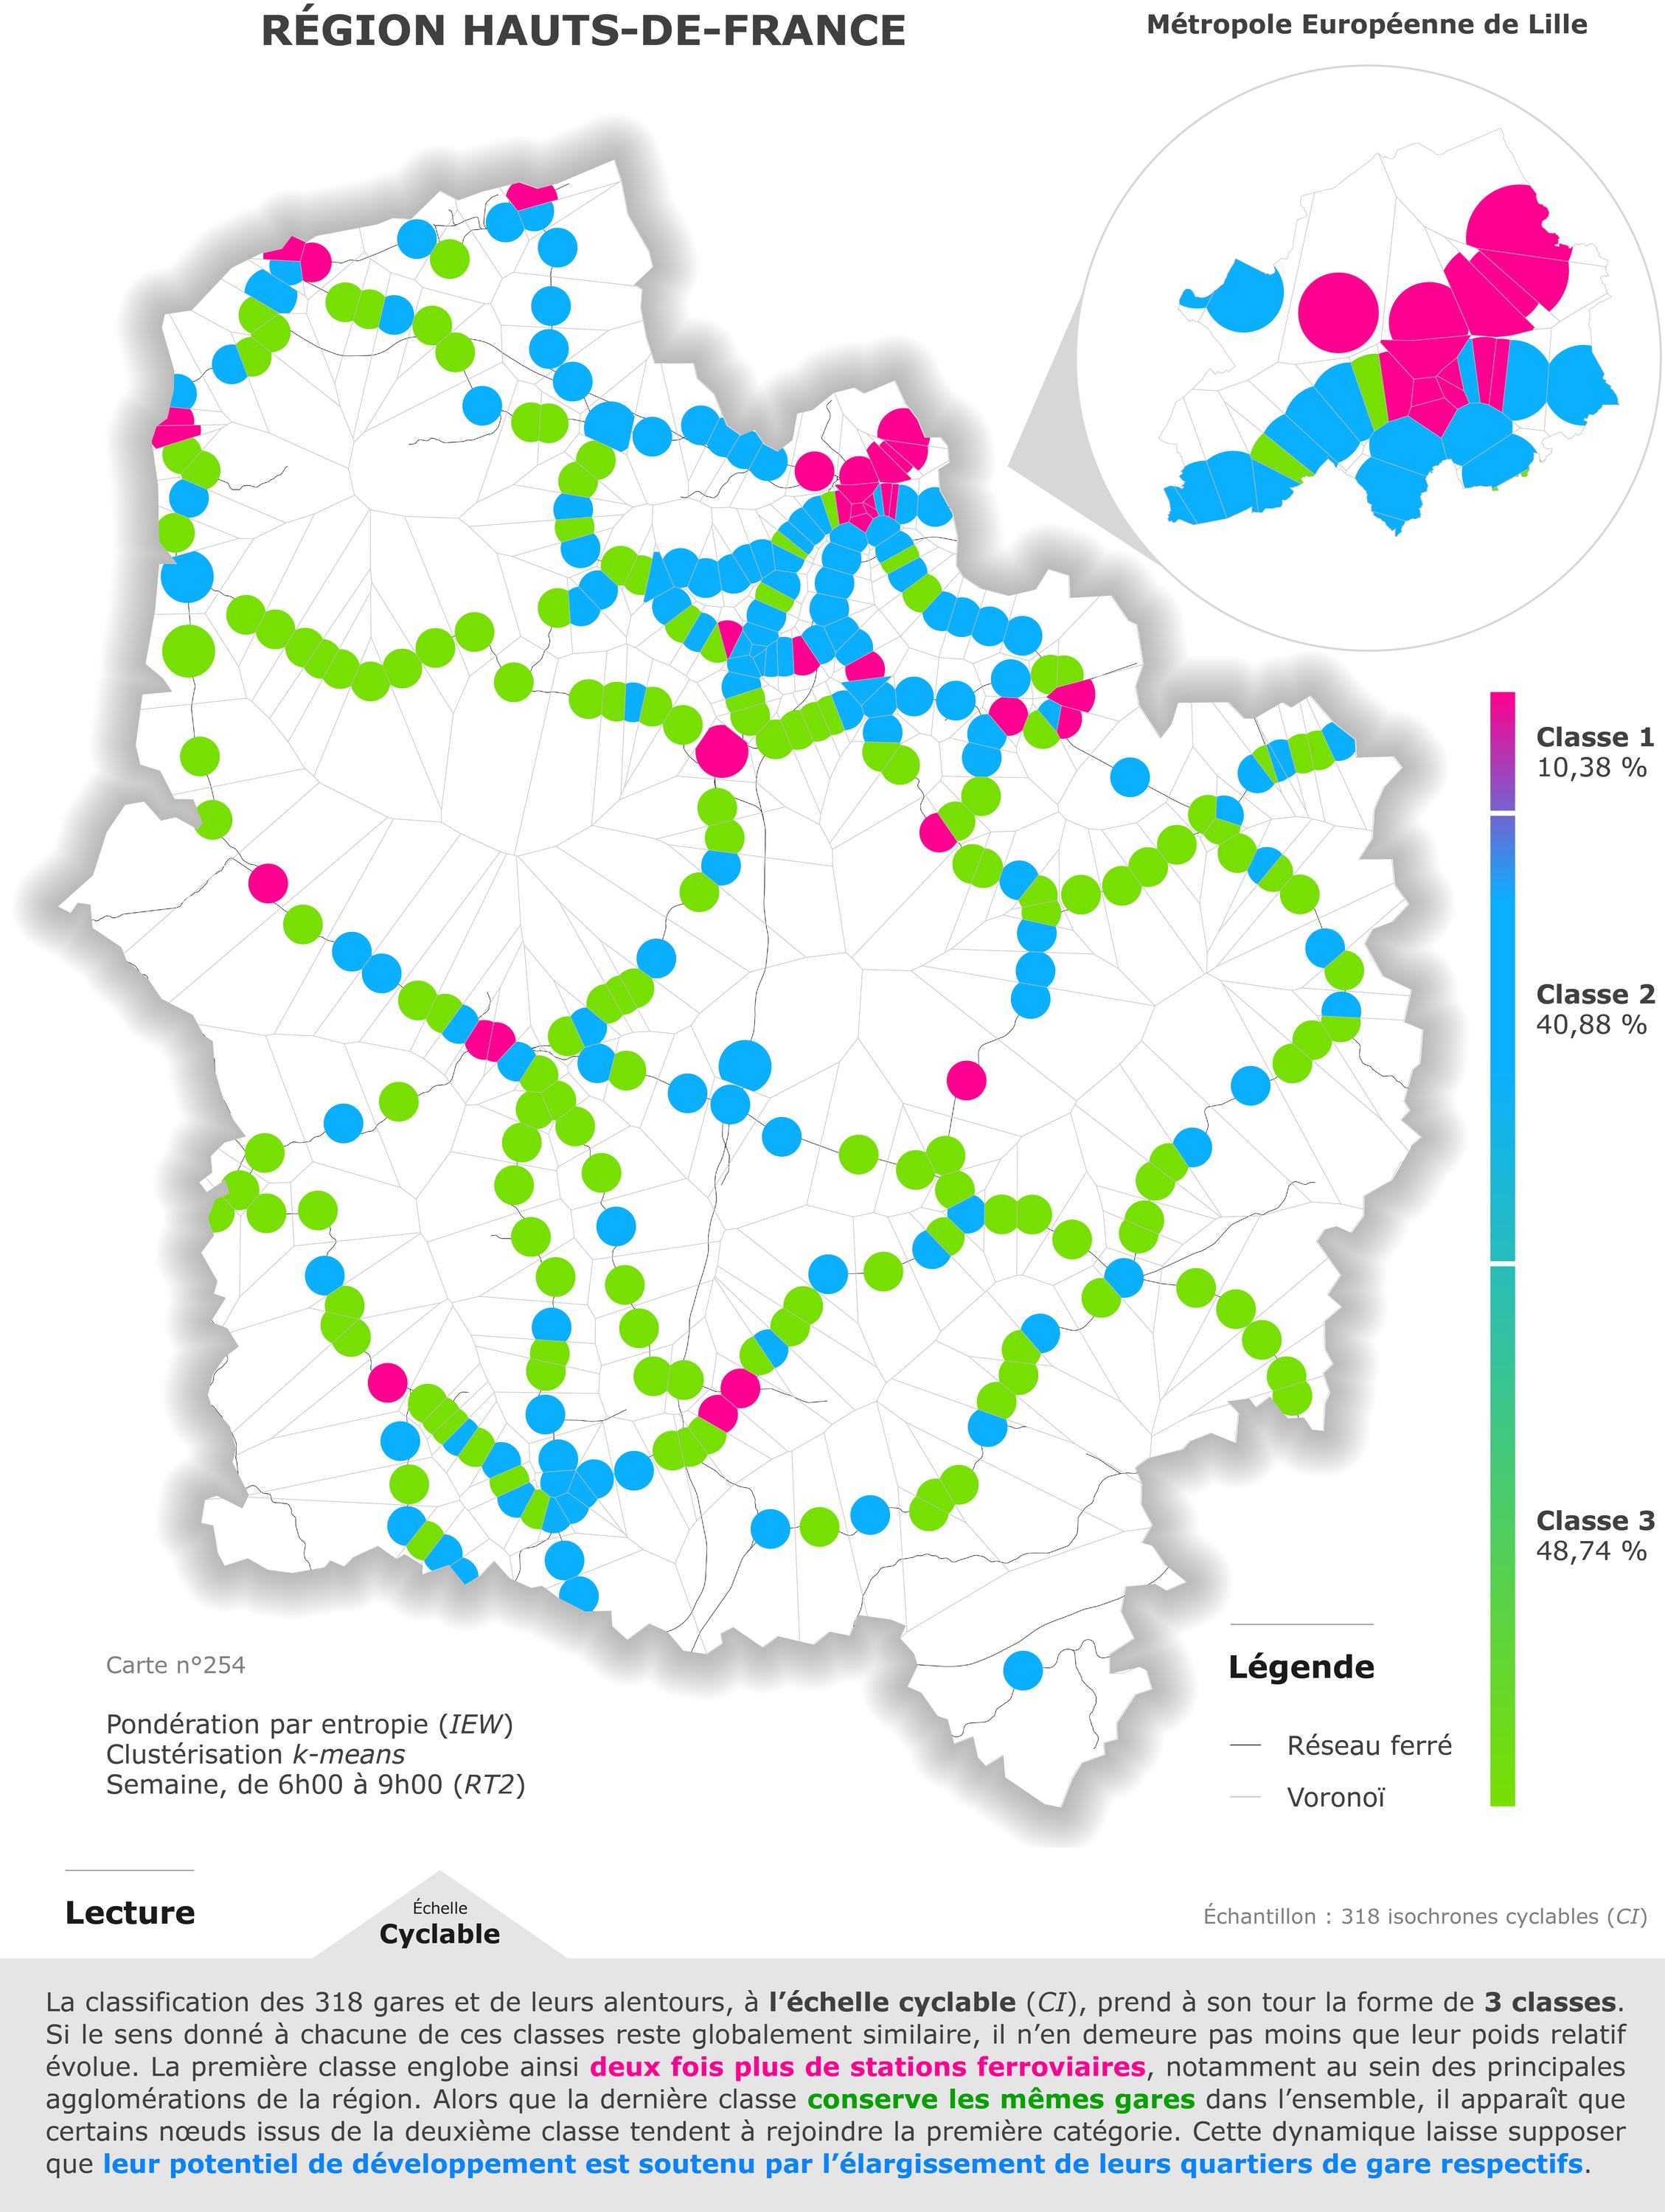
\includegraphics[width=1\columnwidth]{src/Figures/Chap-6/FR_NPART_Carte_Classification_CI.jpg}}
        \vspace{5pt}
        \begin{flushright}\scriptsize{
        Réalisation~: \textcolor{blue}{Dylan Moinse (2024)}
        \\
        Auteur·rice·s~: projet de recherche \acrshort{NPART}
        }\end{flushright}
    \end{carte}

    % Typologie accessibilité dépendante VS classification
Ainsi, l’approche par classification nous permet d’approfondir la caractérisation des stations et de leurs territoires environnants, en dépassant la simple dichotomie entre gares \Guillemets{accessibles} et \Guillemets{non-accessibles}, en particulier grâce à la distinction qui émerge entre les classes \(C2\) et \(C3\). Il est par ailleurs intéressant de noter que la moitié des gares classées dans \(C1\), autant pour \(PI\) que pour \(CI\), sont pourtant positionnées comme \Guillemets{dépendantes}. En effet, sur les 18 et 34 gares classées dans \(C1\) pour \(PI\) et \(CI\) respectivement, 8 et 15 d'entre elles correspondent à des gares en situation de \Guillemets{dépendance}. Ce constat donne à penser que la typologie fondée sur le modèle \acrshort{NPM} originel, non seulement s’avère moins précise, mais s’écarte de la classification statistique réalisée. Ce bilan rejoint les critiques contemporaines formulées dans la littérature scientifique, lesquelles encouragent à s’éloigner d’une interprétation simpliste prenant appui sur une vision strictement diagrammatique.%%Rédigé%%

    % Exemples gares
Du point de vue des distances piétonnières (\(PI\)), les 18 gares classées dans \(C1\)\footnote{
    Parmi celles-ci, 8 sont situées dans la zone de \Guillemets{dépendance}, à savoir Beauvais, Boulogne~–~Tintelleries, Calais Ville, Cambrai, Denain, Lille Porte de Douai, Saint-Quentin et Saint-Roch.
} comprennent Amiens, Arras, Beauvais, Boulogne~–~Tintelleries, Calais Ville, Cambrai, Compiègne, Denain, Dunkerque, le pôle \textsl{Euraflandres}, Lille CHR, Lille Porte de Douai, Pont de Bois, Roubaix, Saint-Quentin, Saint-Roch, Tourcoing et Valenciennes. En comparant la \hyperref[fig-chap6:classification-gares-pieton]{carte~\ref{fig-chap6:classification-gares-pieton}} (page~\pageref{fig-chap6:classification-gares-pieton}) et la \hyperref[fig-chap6:classification-gares-cyclable]{carte~\ref{fig-chap6:classification-gares-cyclable}} (page~\pageref{fig-chap6:classification-gares-cyclable}), 16 gares supplémentaires s'ajoutent à cette liste, exclusivement au regard du périmètre cyclable (\(CI\))\footnote{
    Ces 16 gares sont également considérées comme \Guillemets{dépendantes} à la fois pour \(PI\) et \(CI\), à l'exception de Boulogne-sur-Mer, Croix~–~Wasquehal et La Madeleine qui se positionnent dans la zone d'\Guillemets{accessibilité} à l'échelle cyclable.
}. Ces gares sont~: Abbeville, Annappes, Beau Marais, Boulogne-sur-Mer, Croix~–~Wasquehal, Croix l'Allumette, Hénin-Beaumont, Jaux, La Madeleine, Le Poirier Université, Lezennes, Loos-lez-Lille, Mont de Terre, Pérenchies, Pont de la Deûle et Ronchin. De plus, 10 gares passent de \(C3\) à \(C2\) lorsque nous élargissons les quartiers de gare, à savoir Avion, Coron de Méricourt, Dreuil-lès-Amiens, Étaples~–~Le Touquet, Jeumont, Laon, Les Fontinettes, Louvroil, Thourotte et Villers-Cotterêts.%%Rédigé%%

    % Tableau Classes par Ridership
% Tableau Classes par Ridership
%%Rédigé%%
    \begin{table}[h!]
    \centering
    \renewcommand{\arraystretch}{1.5}
    \resizebox{\columnwidth}{!}{
    \begin{tabular}{p{0.22\columnwidth}p{0.13\columnwidth}p{0.13\columnwidth}p{0.13\columnwidth}p{0.13\columnwidth}p{0.13\columnwidth}p{0.13\columnwidth}}
        %\hline
    \rule{0pt}{15pt} \small{\textbf{\textcolor{blue}{Classes}}} & \small{\textbf{\textcolor{blue}{\(RT_{1}\)}}} & \small{\textbf{\textcolor{blue}{\(RT_{2}\)}}} & \small{\textbf{\textcolor{blue}{\(RT_{3}\)}}} & \small{\textbf{\textcolor{blue}{\(RT_{4}\)}}} & \small{\textbf{\textcolor{blue}{\(RT_{5}\)}}} & \small{\textbf{\textcolor{blue}{\(RT_{6}\)}}}\\
        \hline
    \multicolumn{7}{l}{\textbf{Isochrones piétonnes} (\(PI\))}\\
\multirow{2}{*}{\small{Classe 1 (\(C1\))}} & \small{6,92~\%} & \textbf{\small{5,66~\%}} & \small{5,97~\%} & \textbf{\small{5,97~\%}} & \small{6,29~\%} & \small{5,97~\%}\\
& \small{22} & \textbf{\small{18}} & \small{19} & \textbf{\small{19}} & \small{20} & \small{19}\\
        \hdashline
\multirow{2}{*}{\small{Classe 2 (\(C2\))}} & \small{30,19~\%} & \textbf{\small{46,86~\%}} & \small{45,91~\%} & \textbf{\small{42,14~\%}} & \small{37,11~\%} & \small{33,65~\%}\\
& \small{96} & \textbf{\small{149}} & \small{146} & \textbf{\small{134}} & \small{118} & \small{107}\\
        \hdashline
\multirow{2}{*}{\small{Classe 3 (\(C3\))}} & \small{62,89~\%} & \textbf{\small{47,48~\%}} & \small{48,11~\%} & \textbf{\small{51,89~\%}} & \small{56,60~\%} & \small{60,38~\%}\\
& \small{200} & \textbf{\small{151}} & \small{153} & \textbf{\small{165}} & \small{180} & \small{192}\\
        \hline
    \multicolumn{7}{l}{\textbf{Isochrones cyclables} (\(CI\))}\\
\multirow{2}{*}{\small{Classe 1 (\(C1\))}} & \small{11,32~\%} & \textbf{\small{10,69~\%}} & \small{11,01~\%} & \textbf{\small{12,89~\%}} & \small{5,97~\%} & \small{6,29~\%}\\
& \small{36} & \textbf{\small{34}} & \small{35} & \textbf{\small{41}} & \small{19} & \small{20}\\
        \hdashline
\multirow{2}{*}{\small{Classe 2 (\(C2\))}} & \small{26,42~\%} & \textbf{\small{41,82~\%}} & \small{34,91~\%} & \textbf{\small{36,16~\%}} & \small{32,08~\%} & \small{42,14~\%}\\
& \small{84} & \textbf{\small{133}} & \small{111} & \textbf{\small{115}} & \small{102} & \small{134}\\
        \hdashline
\multirow{2}{*}{\small{Classe 3 (\(C3\))}} & \small{62,26~\%} & \textbf{\small{47,48~\%}} & \small{54,09~\%} & \textbf{\small{50,94~\%}} & \small{61,95~\%} & \small{51,57~\%}\\
& \small{198} & \textbf{\small{151}} & \small{172} & \textbf{\small{162}} & \small{197} & \small{164}\\
        \hline
        \end{tabular}}
    \caption{Composition des trois classes de gares (\(C1\) à \(C3\)) en fonction de la temporalité et de la taille des quartiers de gare.}
    \label{table-chap6:classification-periodes}
        \vspace{5pt}
        \begin{flushleft}\scriptsize{
        \textcolor{blue}{Lecture~:} en jour de semaine de 6h00 à 10h00 (\(RT_{2}\)), la première classe \(C1\) regroupe 18 quartiers de gare accessibles à pied (\(PI\)), soit 5,66~\% du réseau ferroviaire régional. Cette proportion atteint 34 quartiers de gare accessibles en cycle (\(CI\)), soit 10,69~\% de l'échantillon total.
        }\end{flushleft}
        \begin{flushright}\scriptsize{
        Réalisation~: \textcolor{blue}{Dylan Moinse (2024)}
        \\
        Auteur·rice·s~: projet de recherche \acrshort{NPART}
        }\end{flushright}
        \end{table}%%Rédigé%%

    % Gares changeant de classes en fonction de RT
À travers une analyse plus dynamique fondée sur la temporalité des flux, nous constatons une légère évolution de la classification. Nous avons ainsi examiné la répartition des gares au sein des classes définies selon le référentiel \(RT_{2}\) (voir le \hyperref[table-chap6:classification-periodes]{tableau~\ref{table-chap6:classification-periodes}}, page~\pageref{table-chap6:classification-periodes}). Il est alors intéressant de noter que, bien que la proportion de \(C1\) demeure relativement stable autour de 6~\% pour l’échelle piétonne (\(PI\)), celle-ci fluctue entre 6~\% et 13~\% à l’échelle cyclable (\(CI\)). Toutefois, la classe présentant la plus forte variation est sans aucun doute \(C2\), particulièrement aux moments de \(RT_{2}\) et \(RT_{4}\), correspondant respectivement aux heures de pointe matinales et aux heures de retour. En effet, les parts de \(C2\) sont plus élevées durant les périodes d’affluence et pour \(CI\), ce qui indique une attractivité accrue des gares dans ces contextes spatio-temporels. Ainsi, l’analyse temporelle de la classification révèle des fluctuations dans la composition des classes selon les périodes, avec une proportion plus importante de gares se rapprochant des classes orientées vers le \acrshort{TOD} lorsque les quartiers de gare sont étendus et en période de pointe.%%Rédigé%%

    % Méthodologie Séquences ADN
Dans une perspective visant à obtenir une vision plus systémique des changements d’appartenance des gares aux différentes classes, nous avons adopté la démarche développée par \textcolor{blue}{\textcite[518]{caset_measuring_2018}}\index{Caset, Freke|pagebf}\index{Vale, David~S.|pagebf}\index{Viana, Cláudia~M.|pagebf}, qu’iels ont nommée \Guillemets{séquence ADN des gares} (\textsl{DNA sequence}). Cette approche permet de représenter l’appartenance des gares à leurs clusters en fonction de la variation de la taille de leur quartier. La \Guillemets{séquence ADN des gares}, que nous notons \(ADN\), repose sur une succession ordonnée de classes auxquelles chaque gare est associée, en fonction des échelles temporelles (\(RT_{1}\) à \(RT_{6}\)) et géographiques (\(PI\) et \(CI\)) considérées (voir la \hyperref[equation:sequence-adn]{formule~\ref{equation:sequence-adn}}, page~\pageref{equation:sequence-adn}). À titre d’exemple, le pôle \textsl{Euraflandres} présente une séquence stable, notée \Guillemets{\(C1C1C1C1C1C1-C1C1C1C1C1C1\)}, témoignant d'une constance dans son appartenance à \(C1\) à travers les différents axes spatio-temporels.%%Rédigé%%

    % Équation séquences ADN gares
\begin{equation}
\label{equation:sequence-adn}
\begin{aligned}
ADN_k = \sum_{k=1}^{6} \left( C^{RT_k}_{PI} + C^{RT_k}_{CI} \right)
\end{aligned}
\end{equation}
\begin{align*}
    &\text{où~:} \\
    &ADN_i \text{ est la séquence ADN de la gare}~i\text{.}\\
\end{align*}%%Rédigé%%

    % Résultats Séquences ADN
Finalement, pratiquement autant de combinaisons que de gares sont observées, soit pas moins de 263 séquences uniques à travers le réseau ferroviaire pour les 12 composantes analysées. Ce résultat montre que seulement 1,89~\% des gares conservent toujours la même classe d'appartenance, une proportion qui diverge avec l'analyse statistique de \textcolor{blue}{\textcite[518]{caset_measuring_2018}}\index{Caset, Freke|pagebf}\index{Vale, David~S.|pagebf}\index{Viana, Cláudia~M.|pagebf}, selon laquelle 49~\% des gares belges sont assignées à une typologie constante, que le rayon soit de 0,7~; 0,8~; 1,2 ou 3,0 kilomètres. Toutefois, plusieurs chaînes récurrentes peuvent être citées~: 
\begin{customitemize}
    \item \Guillemets{\(C2C2C2C2C2C2-C2C2C2C2C2C2\)}, représentant des gares entièrement dans~\(C2\)~;
    \item \Guillemets{\(C2C2C2C2C2C2-C1C1C1C1C1C1\)}, correspondant aux gares qui passent de \(C2\) dans le contexte de \(PI\) à \(C1\) pour \(CI\) sur l'ensemble des périodes~;
    \item \Guillemets{\( C3C3C3C3C3C3-C2C2C2C2C2 \textcolor{blue}{C3} \)}, désignant les gares qui passent de \(C3\) à \(C2\) sur tous les intervalles temporels à l'exception du week-end.
\end{customitemize}%%Rédigé%%

    % Transition
Poursuivant l'exploration de la typologie ainsi obtenue, et après avoir clarifié la répartition des gares au sein de chaque catégorie, nous entreprenons à présent une analyse détaillée de ces classes. La dernière sous-section qui suit fournit une définition des catégories identifiées dans une perspective aménagiste, en s’appuyant sur une analyse statistique des facteurs déterminants. Ce cadre interprétatif permet non seulement de saisir les spécificités propres à chaque classe, mais aussi d'offrir une lecture conceptuelle des distinctions observées, éclairant les logiques spatiales et fonctionnelles qui sous-tendent cette classification régionale.%%Rédigé%%

    % 6.4.3.2.
    \needspace{1\baselineskip} % Réserve de l'espace
\subsubsection*{De la définition à l'interprétation des catégories établies
    \label{chap6:results-classification-gares-indicateurs}
    }

    % Méthodologie Radars PI et CI et séquence ADN
Afin de définir les catégories de manière aussi fidèle que possible aux données statistiques, tout en offrant un cadre d’opérationnalisation et de communication simplifié, nous avons choisi de nous inspirer du \Guillemets{modèle papillon} (\textsl{butterfly model}) comme cadre visuel d’analyse de référence. Cette représentation conceptuelle a été reprise pour illustrer le \acrshort{NPM} dans la thèse de doctorat de \textcolor{blue}{Freke} \textcolor{blue}{\textcite[52]{caset_planning_2019}}\index{Caset, Freke|pagebf}, qui l’a appliquée aux stations belges de Waterloo, Watermael et Buggenhout, en s’appuyant sur les modèles initiaux développés par la Province de \textcolor{blue}{\textcite{hollande-septentrionale_maak_nodate}}\index{Province de Hollande-Septentrionale@\textsl{Province de Hollande-Septentrionale}|pagebf}\index{Association Deltametropolis@\textsl{Association Deltametropolis}|pagebf}.%%Rédigé%%

    % Résultats Radars PI et CI - général
À partir des \hyperref[fig-chap6:radar-pi]{diagrammes en radar~\ref{fig-chap6:radar-pi}} et\hyperref[fig-chap6:radar-ci]~\ref{fig-chap6:radar-ci} (pages~\pageref{fig-chap6:radar-pi} et~\pageref{fig-chap6:radar-ci}) divisés en quatre axes constituant le modèle \acrshort{NPART}, nous avons la possibilité de comparer non seulement les valeurs normalisées et pondérées de chaque dimension et variable, mais également les deux types de quartiers de gare. Il ressort ainsi que les dimensions relatives à la fréquentation des gares durant les heures de pointe matinales (\(RT_{2}\)) et à la concentration et à la diversification des fonctions urbaines (\(P\)) présentent globalement les valeurs les plus faibles. Cette observation statistique suggère qu'une partie des gares compense une intensité urbaine faible par une accessibilité plus forte. Dans ce cas précis, la contribution de l'intensité urbaine à la fréquentation est faible dans ce nombreux cas, ce qui montre un potentiel de développement par intensification urbaine. Toutefois, les indicateurs les plus faibles se situent presque tous dans la dimension liée à la connectivité locale (\(A\)), notamment en ce qui concerne la desserte en métro et en tramway (\(A_{7}\)), en \acrshort{VLS} (\(A_{6}\)), l'offre de stationnement vélo (\(A_{5}\)) et la longueur du réseau cyclable (\(A_{4}\)), pour les périmètres piétonniers (\(PI\)) comme cyclables (\(CI\)), laissant supposer que les connexions douces restent largement marginalisées.%%Rédigé%%

    % Figure Radar PI
    \begin{figure}[h!]\vspace*{4pt}
        \caption{Graphique en radar des indicateurs du modèle par classe de quartier de gare piéton (\(PI\)).}
        \label{fig-chap6:radar-pi}
        \centerline{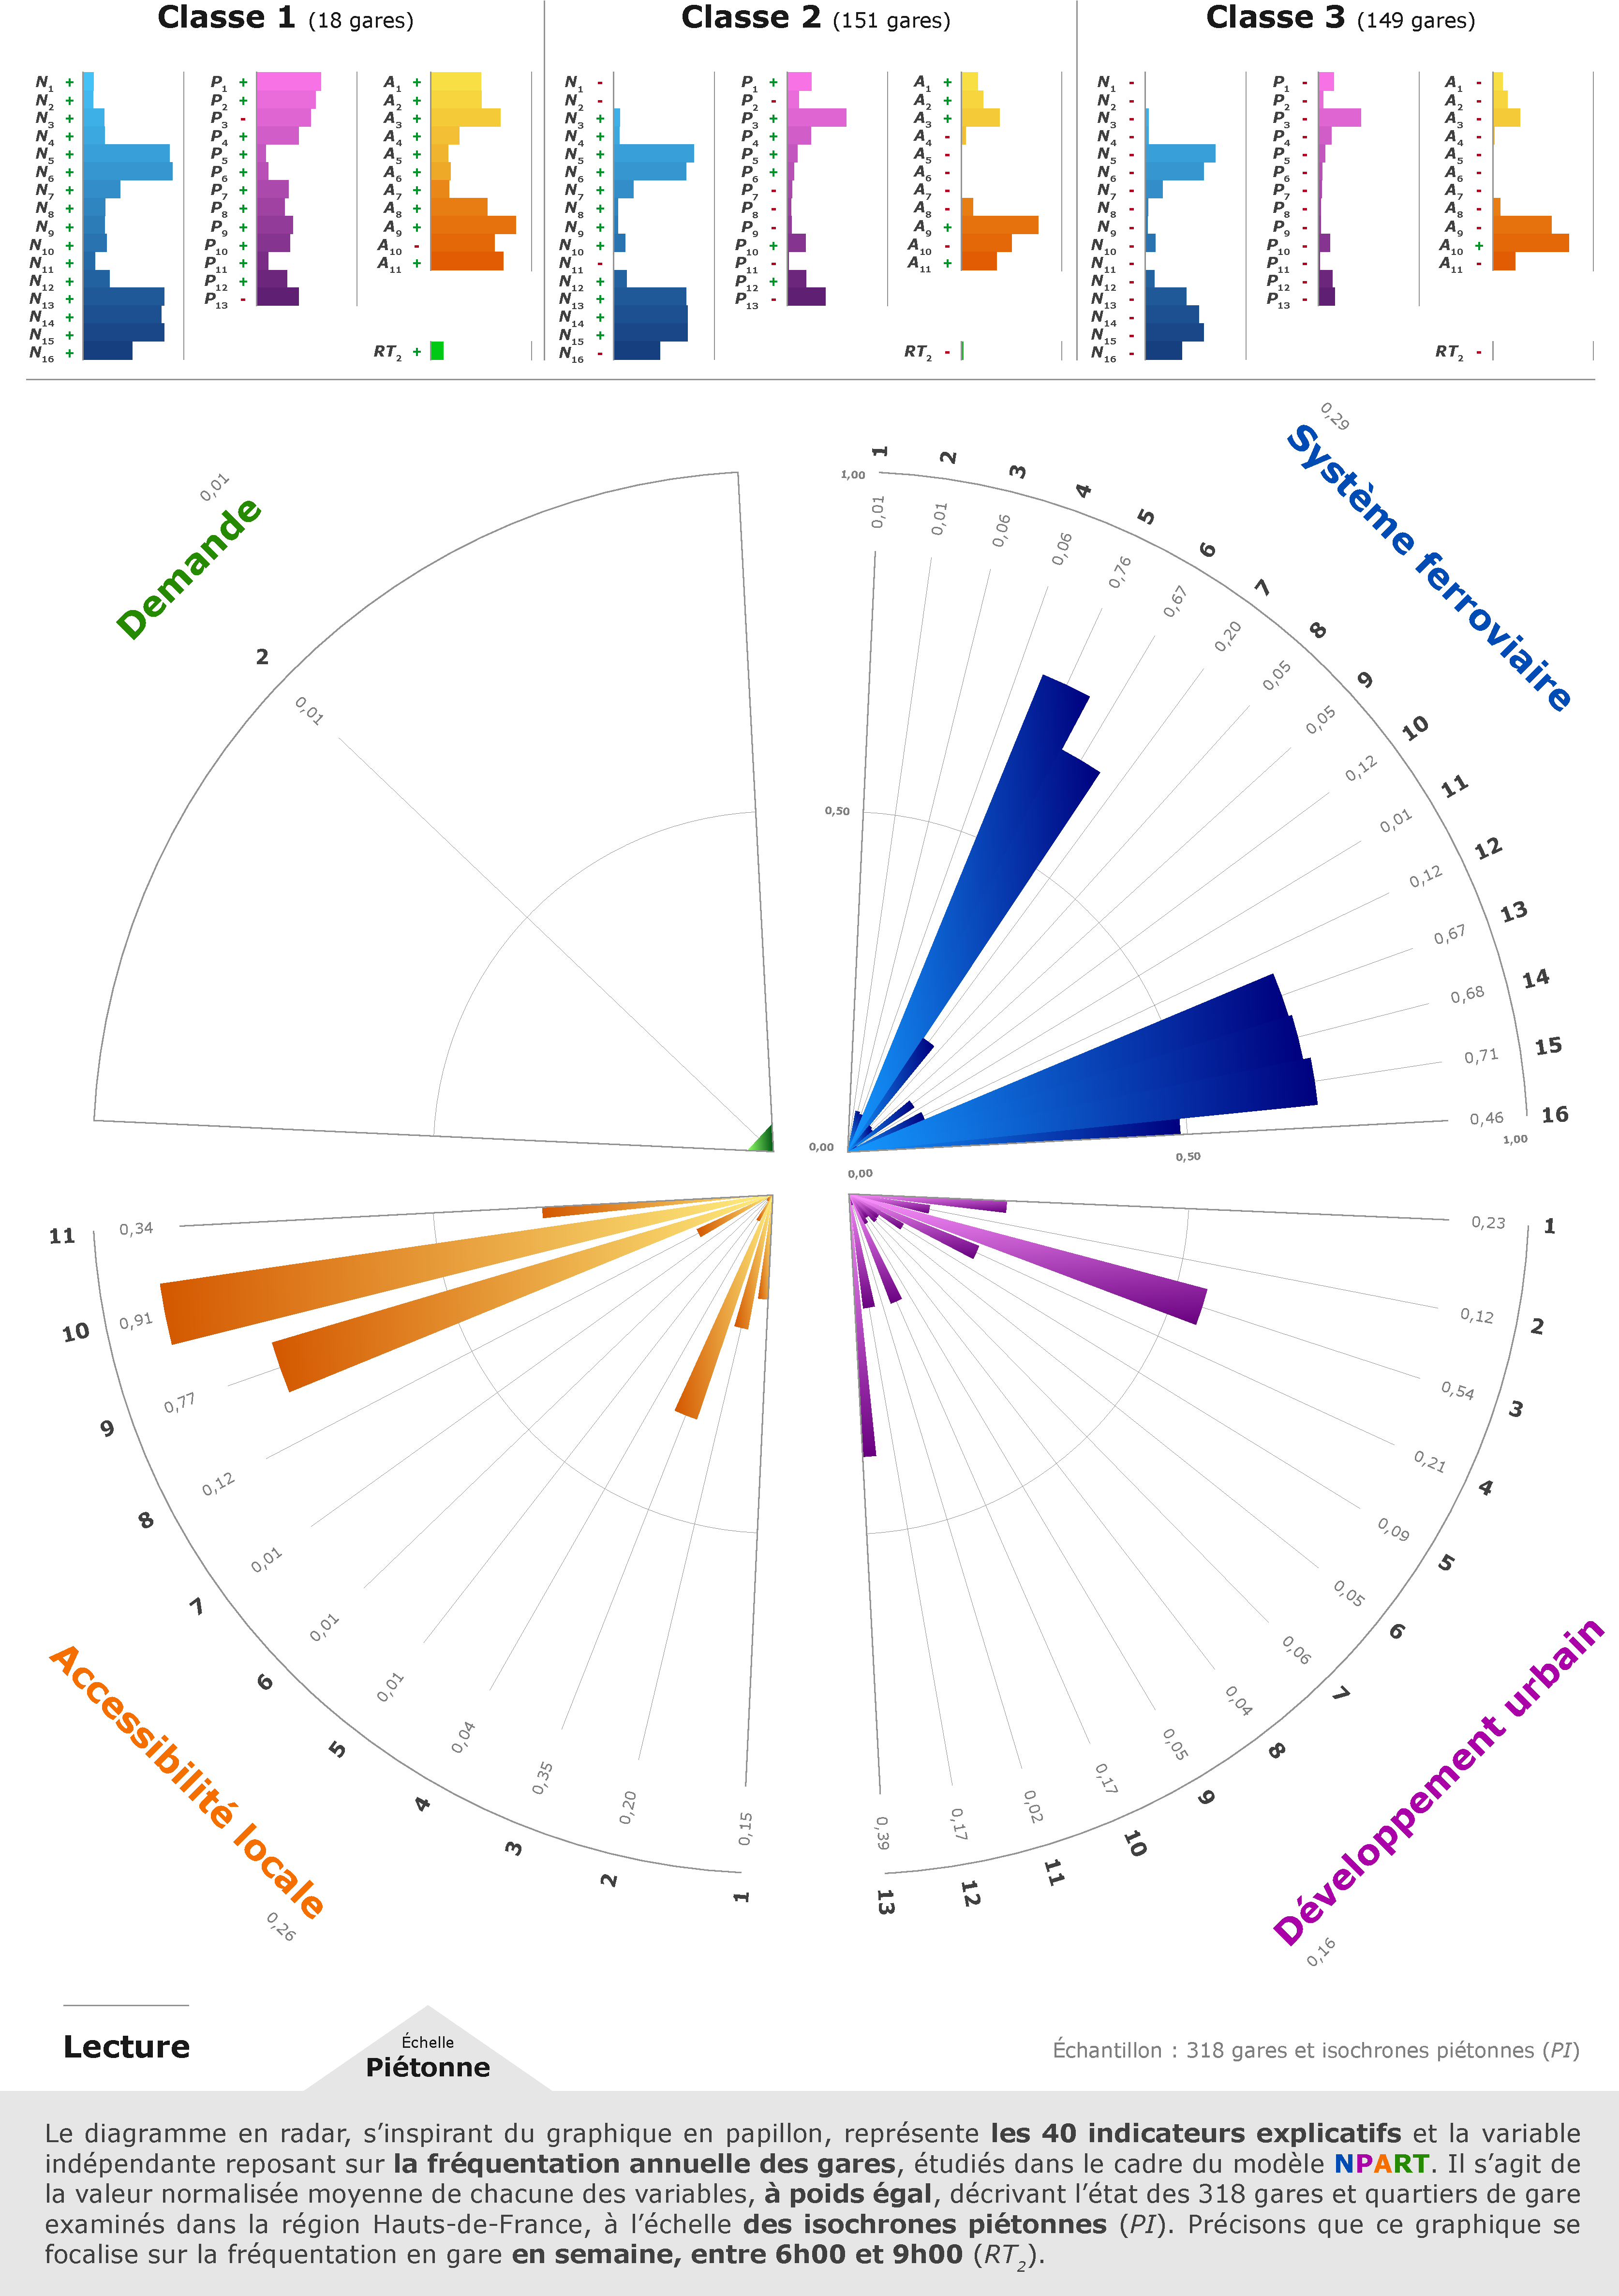
\includegraphics[width=1\columnwidth]{src/Figures/Chap-6/FR_NPART_Radar_PI.pdf}}
        \vspace{5pt}
        \begin{flushright}\scriptsize{
        Réalisation~: \textcolor{blue}{Dylan Moinse (2024)}
        \\
        Auteur·rice·s~: projet de recherche \acrshort{NPART}
        }\end{flushright}
    \end{figure}

    % Figure Radar CI
    \begin{figure}[h!]\vspace*{4pt}
        \caption{Graphique en radar des indicateurs du modèle par classe de quartier de gare cyclable (\(CI\)).}
        \label{fig-chap6:radar-ci}
        \centerline{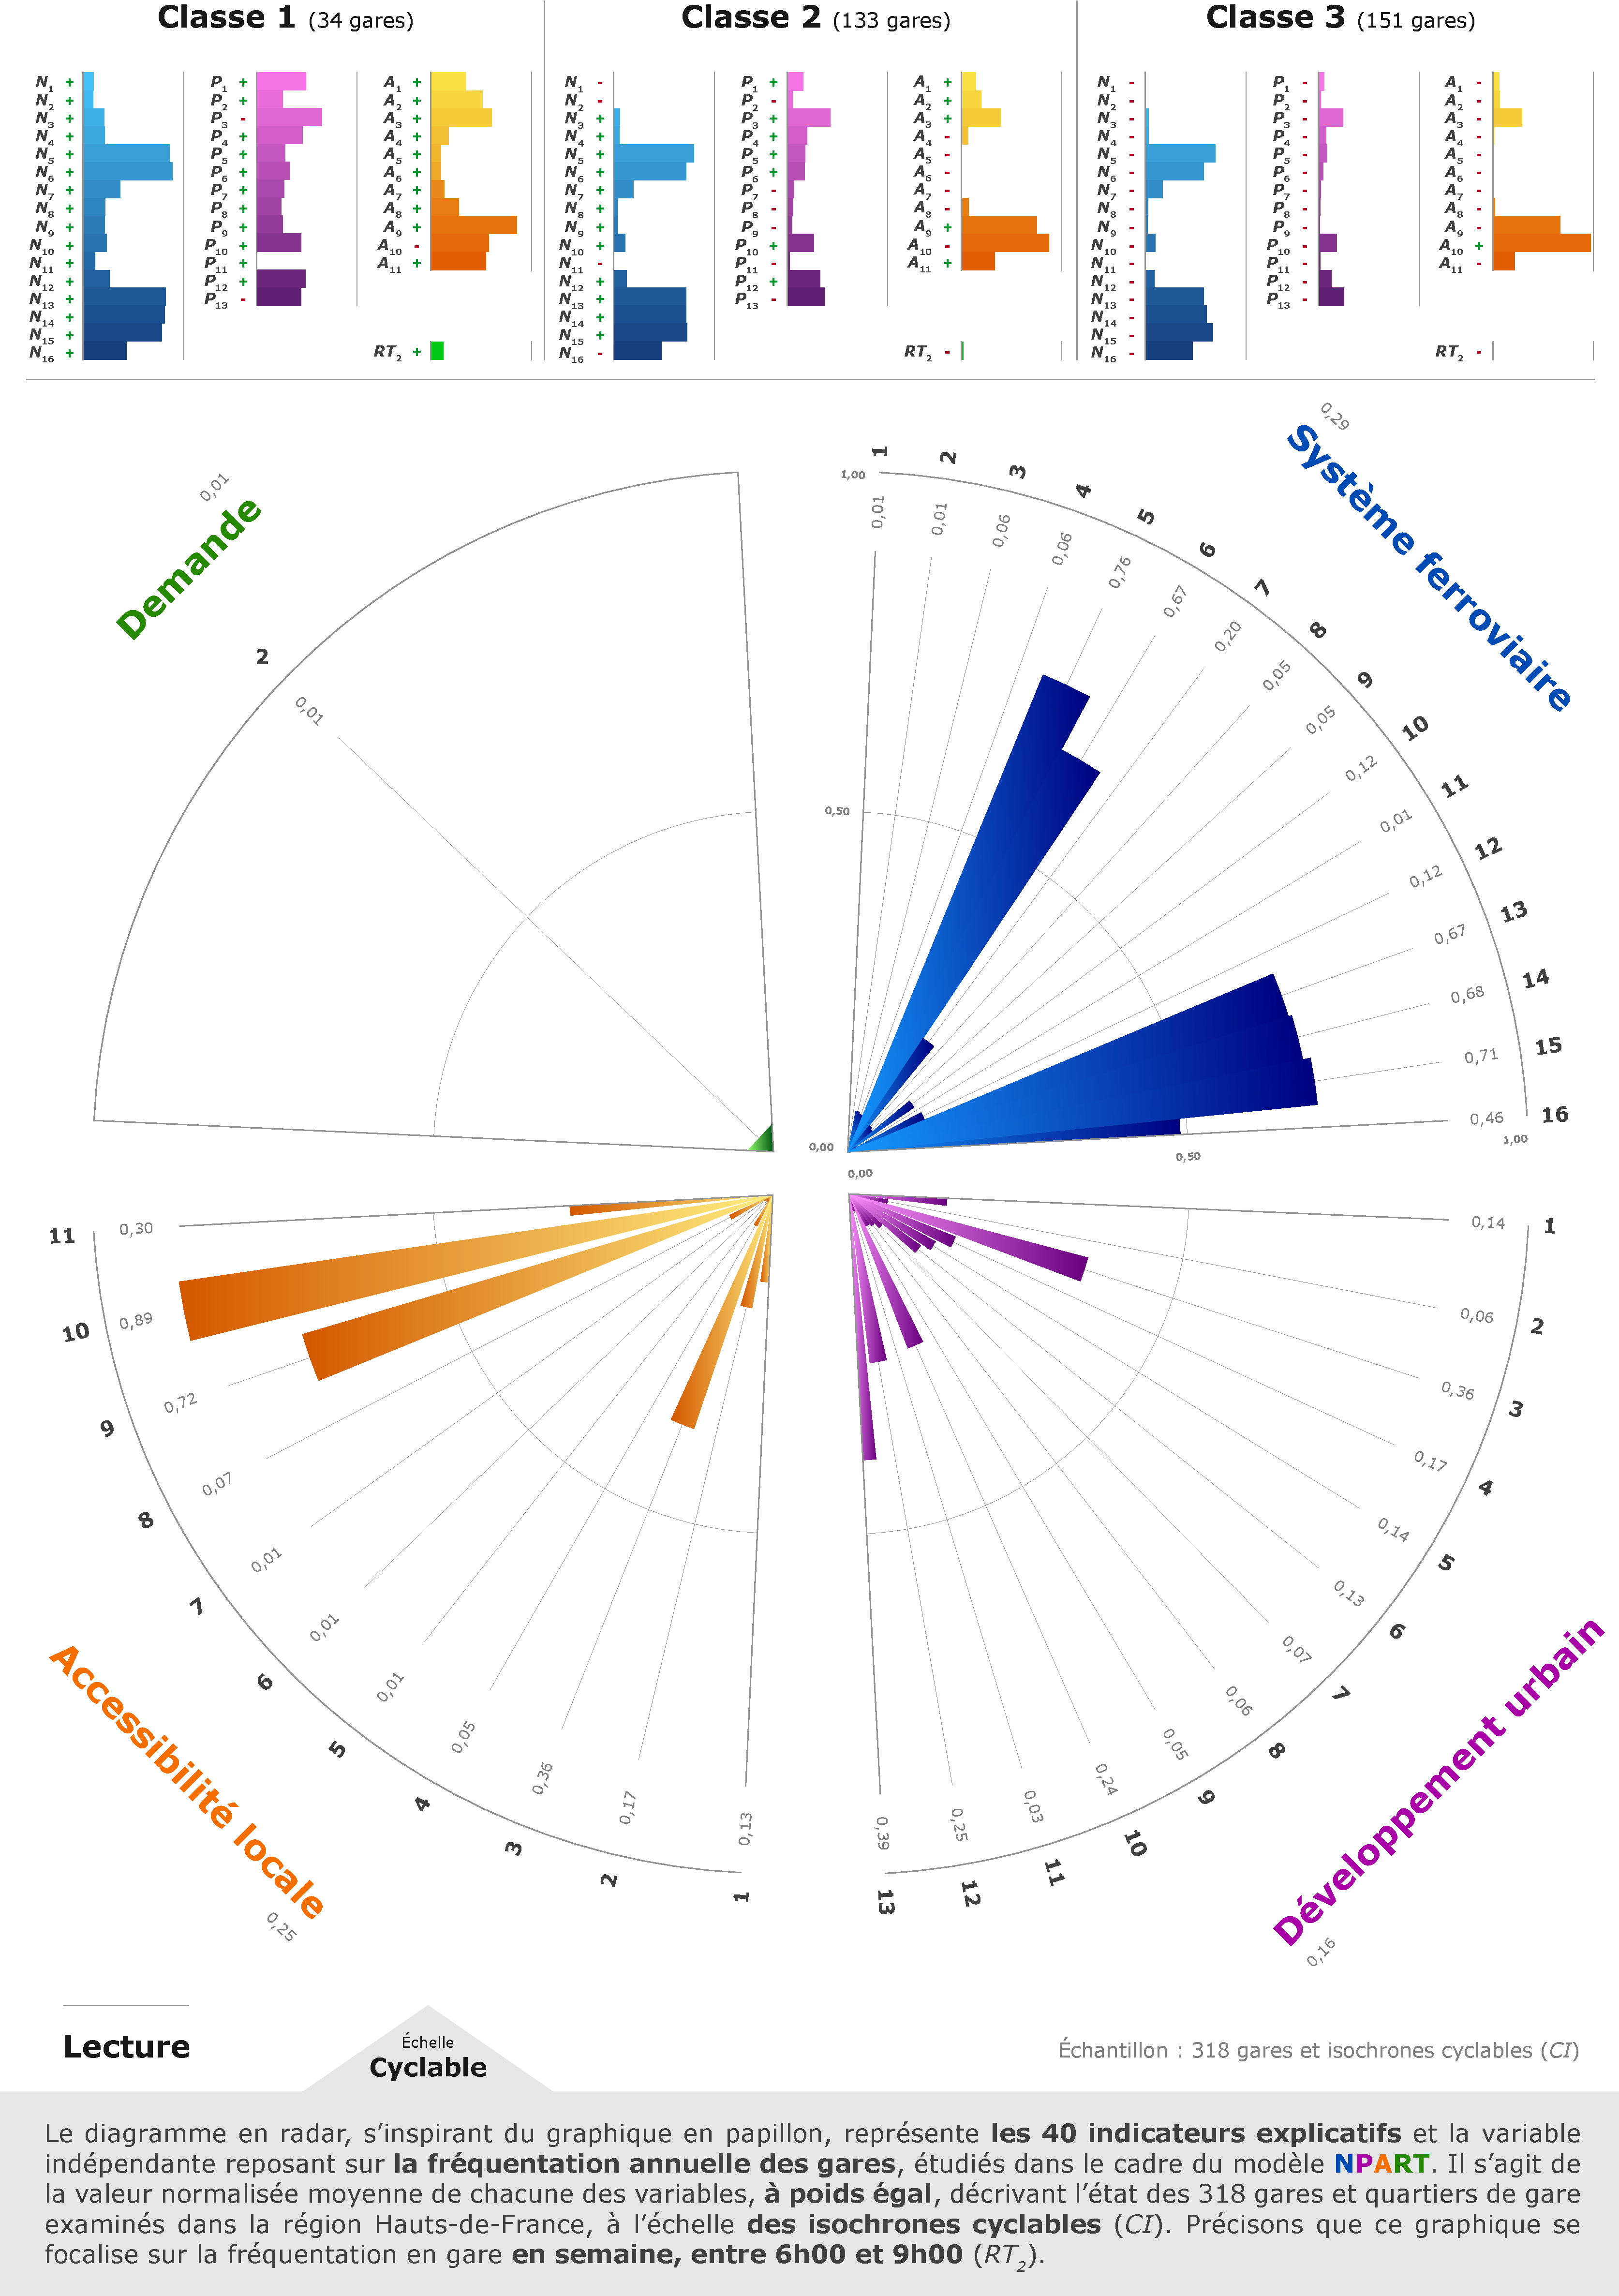
\includegraphics[width=1\columnwidth]{src/Figures/Chap-6/FR_NPART_Radar_CI.pdf}}
        \vspace{5pt}
        \begin{flushright}\scriptsize{
        Réalisation~: \textcolor{blue}{Dylan Moinse (2024)}
        \\
        Auteur·rice·s~: projet de recherche \acrshort{NPART}
        }\end{flushright}
    \end{figure}

    % Résultats Radards PI et CI - différence
En moyenne, les critères du \acrshort{NPART} enregistrent un gain de 7~\% entre \(PI\) et \(CI\), toutes dimensions confondues. En excluant les dimensions \(N\) et \(RT\), pour lesquelles l'échelle géographique n'a pas d'influence, la croissance moyenne atteint 12~\%, ce qui suggère que l’extension des quartiers de gare tend à lisser les disparités entre les différents territoires couverts par le réseau ferroviaire. En élargissant les périmètres des quartiers de gare, il apparaît que 14 indicateurs voient leur valeur relative augmenter, en particulier dans la dimension \(P\)~: la présence d'espaces verts (\(P_{6}\), +144~\%), la valeur foncière des activités industrielles (\(P_{11}\), +61~\%), la spécialisation industrielle et commerciale (\(P_{5}\), +59~\%), la proportion de logements sociaux (\(P_{12}\), +48~\%), la valeur foncière résidentielle (\(P_{10}\), +41~\%), le nombre de \acrshort{POIs} \Guillemets{intermédiaires} (\(P_{8}\), +35~\%), de \Guillemets{proximité} (\(P_{11}\), +20~\%) et \Guillemets{supérieurs} (\(P_{9}\), +7~\%), ainsi que le revenu des foyers (\(P_{13}\), +1~\%). À l’inverse, 10 indicateurs perdent en valeur relative, principalement dans la dimension \(A\)~: la desserte en bus (\(A_{8}\), -43~\%), la longueur du réseau piéton (\(A_{1}\), -18~\%), le coefficient d'accessibilité par rapport au taux de couverture théorique (\(A_{2}\), -16~\%), le taux de ménages non motorisés (\(A_{11}\), -11~\%), les limites de vitesse motorisée (\(A_{9}\), -6~\%) et la restriction du stationnement automobile (\(A_{10}\), -3~\%).%%Rédigé%%

    % Résultats Radars PI et CI - classes
En filtrant ces valeurs selon la classe d’appartenance des gares, nous sommes en mesure de définir avec une plus grande précision chacune des catégories présentées (voir les \hyperref[fig-chap6:radar-pi]{diagrammes en radar~\ref{fig-chap6:radar-pi}} et\hyperref[fig-chap6:radar-ci]~\ref{fig-chap6:radar-ci}, pages~\pageref{fig-chap6:radar-pi} et~\pageref{fig-chap6:radar-ci})~:
\begin{customitemize}
    \item \(C1\) a les valeurs moyennes pondérées les plus élevées pour toutes les dimensions, suggérant que cette classe a les meilleures performances et un certain \Guillemets{équilibre} selon les paramètres mesurés. Au niveau de \(PI\), \(N\) atteint 0,42, \(P\) 0,35, \(A\) 0,47 et \(RT_{2}\) 0,10. Pour \(CI\), \(N\) s'établit à 0,36, \(P\) à 0,35, \(A\) à 0,38 et \(RT_{2}\) à 0,06~;
    \item \(C2\) montre des valeurs se situant entre \(C1\) et \(C3\). Au niveau de \(PI\), \(N\) est égale à 0,31, \(P\) à 0,17, \(A\) à 0,23 et \(RT_{2}\) à 0,01. Pour \(CI\), \(N\) atteint 0,31, \(P\) 0,18, \(A\) 0,26 et \(RT_{2}\) 0,01~;
    \item \(C3\) a les valeurs les plus basses. Au niveau de \(PI\), \(N\) est de 0,22, \(P\) de 0,12, \(A\) de 0,20 et \(RT_{2}\) de 0,00. Pour \(CI\), \(N\) est de 0,25, \(P\) de 0,10, \(A\) de 0,21 et \(RT_{2}\) de 0,00.
\end{customitemize}%%Rédigé%%

    % Interprétation classes
À la lumière de ces données, nous avons la capacité de donner un sens plus précis à cette classification dans le cadre régional de notre terrain empirique. À ce stade, il convient de considérer que la classe \(C1\) regroupe les gares et leurs environnements urbains accessibles à pied ou à vélo qui adhèrent ou s’approchent des principes d’aménagement du \acrshort{TOD} et du \acrshort{M-TOD}. La classe \(C2\) recèle quant à elle un potentiel d’aménagement \acrshort{TOD}, sous certaines conditions que nous expliciterons. Enfin, la classe \(C3\) rassemble les stations qui sont à la fois mal desservies, relativement peu développées et insuffisamment aménagées pour favoriser les systèmes de mobilité alternative.%%Rédigé%%

    % Classe C1
La première classe, \(C1\), affiche des scores remarquablement élevés dans les quatre dimensions qui composent le \acrshort{NPART}, positionnant ainsi ces gares comme les candidats les plus proches du modèle \acrshort{TOD} et de sa déclinaison, comparativement à ce qui est présent dans le réseau étudié. Cette classe se distingue avant tout par de meilleures connexions cyclables au sein des espaces publics, une position stratégique au sein du réseau technique et une forte attractivité industrielle et commerciale. Les critères les plus saillants, caractérisant cette classe par leur écart de valeurs avec les autres regroupements, sont les suivants~:
\begin{customitemize}
    \item \textsl{Infrastructure cyclable}\footnote{
        Les quartiers de gare \(C1\) sont connectés à une flotte moyenne de 120 (\(PI\)) et 243 vélos partagés (\(CI\)). Le réseau cyclable est long de 670 (\(PI\)) et 1~378 kilomètres (\(CI\)).
    }. Les services de \acrshort{VLS} (\(A_{6}\)) y sont respectivement 42 et 191 fois plus nombreux par rapport à \(C2\) et \(C3\) pour \(PI\) et 58 et 1~014 fois pour \(CI\). De plus, la longueur du réseau cyclable (\(A_{5}\)) est 22 et 60 fois (\(PI\)) et 14 et 126 fois supérieure (\(CI\))~;
    \item \textsl{Transports en commun urbains sur rail}\footnote{
        Environ 2 (\(PI\)) et 4 arrêts de métro et de tramway (\(CI\)) desservent les quartiers de gare \(C1\).
    }. La desserte en métro et en tramway (\(A_{7}\)) est 89 fois (\(PI\)) et 115 fois (\(CI\)) plus élevée par rapport \(C2\), alors que \(C3\) n'en bénéficie pas~;
    \item \textsl{Système à grande vitesse}\footnote{
        En semaine, 9 (\(PI\)) et 5 \acrshort{TGV} (\(CI\)) desservent les gares \(C1\), contre 8 et 4 \acrshort{TGV} le week-end.
    }. La fréquence des \acrshort{TGV} est 19 et 91 fois (\(PI\)) et 10 et 257 fois au-dessus (\(CI\)) en semaine (\(N_{1}\)) et 19 et 113 fois (\(PI\)) et 10 et 206 fois au-dessus (\(CI\)) le week-end (\(N_{2}\)) face aux autres classes~;
    \item \textsl{Morphologie du réseau ferré}\footnote{
        La centralité d'intermédiarité des gares \(C1\) est égale à 0,012 (\(PI\)) et 0,007 (\(CI\)).
    }. La centralité d'intermédiarité (\(N_{11}\)) est 8 et 28 fois (\(PI\)) et 4 et 20 fois (\(CI\)) plus importante~;
    \item \textsl{Estimation des terrains à usage industriel, commercial et de bureau}\footnote{
        Les terrains à usage industriel, commercial et de bureau valent 17~704 (\(PI\)) et 7~033~\euro~par mètre carré (\(CI\)) au sein des quartiers de gare \(C1\).
    }. La valeur foncière des secteurs secondaire et tertiaire (\(P_{11}\)) est 9 à 12 fois (\(PI\)) et 4 à 6 fois plus élevée (\(CI\))~;
    \item \textsl{Flux}\footnote{
        Au cours des heures de pointe du matin, les gares \(C1\) sont fréquentées chaque année par plus de 854~511 (\(PI\)) et 475~508 voyageur·se·s (\(CI\)).
    }. Enfin, la fréquentation des gares en période d'affluence matinale (\(RT_{2}\)) est 8 et 57 fois (\(PI\)) et 4 et 57 fois plus élevée (\(CI\)) que pour \(C2\) et \(C3\).
\end{customitemize}%%Rédigé%%

    % Classe C2 - partie 1
Si \(C1\) affiche des valeurs moyennes pondérées nettement supérieures à celles de \(C2\) avec des écarts de 103~\% pour \(P\) (\(PI\)) et de 92~\% (\(CI\)), de 103~\% pour \(A\) (\(PI\)) et de 50~\% (\(CI\)), ainsi que de 815~\% pour \(RT_{2}\) (\(PI\)) et de 343~\% (\(CI\)), l’écart se réduit pour \(N\), atteignant seulement 36~\% (\(PI\)) et 16~\% (\(CI\)). Ces écarts soulèvent donc un questionnement pertinent quant à l’identité de \(C2\). Les principales dissemblances se manifestent dans le traitement des espaces publics~:
\begin{customitemize}
    \item \textsl{Réseau ferroviaire plutôt performant}\footnote{
        Les gares \(C2\) sont desservies par 38 (\(PI\)) et 41 \acrshort{TER} (\(CI\)) par jour de semaine, contre 15 et 17 \acrshort{TER} un jour de week-end. En moyenne, 16 heures et 14 heures (\(PI\) et \(CI\)) s'écoulent entre le départ du premier et du dernier train, respectivement la semaine et le week-end. En termes d'accessibilité inter-nodale, pour un budget temps d'une heure, 2 autres gares (\(PI\) et \(CI\)) sont accessibles depuis une gare \(C2\). Pour rejoindre Euralille, il faut généralement traverser 4 gares (\(PI\) et \(CI\)) en 62 minutes (\(PI\) et \(CI\)), contre 6 gares (\(PI\) et \(CI\)) en 110 (\(PI\)) et 112 minutes (\(CI\)) pour Châtelet.
    }. Concernant \(N\), la fréquence des lignes \acrshort{TER} (\(N_{3}\) et \(N_{4}\)) demeure élevée avec un écart peu prononcé par rapport à la première classe. L’amplitude horaire (\(N_{5}\) et \(N_{6}\)) est presque similaire, tout comme le nombre de gares accessibles en une heure (\(N_{12}\)) et l’accessibilité vers les pôles urbains majeurs (\(N_{13}\), \(N_{14}\), \(N_{15}\) et \(N_{16}\))~;
    \item \textsl{Attractivité résidentielle et faible densité d'activités}\footnote{
        Les quartiers de gare \(C2\) sont investis par 3~085 (\(PI\)) et 1~473 habitant·e·s par kilomètre carré (\(CI\)), contre 398 (\(PI\)) et 175 emplois par kilomètre carré (\(CI\)). 8~\% (\(PI\)) et 6~\% (\(CI\)) des aires d'influence \(C2\) sont occupées par des activités commerciales. Nous comptabilisons 44 (\(PI\)) et 116 \acrshort{POIs} de \Guillemets{proximité} (\(CI\)), 22 et 56 de gamme \Guillemets{intermédiaire}, ainsi 7 et 20 de type \Guillemets{supérieur}.
    }. Du côté de \(P\), la densité de population (\(P_{1}\)) varie peu, contrairement à la densité d’emplois (\(P_{2}\)) et à l'usage commercial des sols (\(P_{4}\)), et un écart notable est observé pour les \acrshort{POIs} (\(P_{7}\), \(P_{8}\) et \(P_{9}\))~;
    \item \textsl{Fragmentation des connexions entre réseaux et territoires}\footnote{
        Les quartiers de gare \(C2\) sont connectés à une flotte moyenne de 0 (\(PI\)) et 4 vélos partagés (\(CI\)). Le réseau cyclable est long de 29 (\(PI\)) et 64 kilomètres (\(CI\)), contre 47 et 113 kilomètres pour le réseau piéton. La superficie des places de parking automobile est égale à 43~209 (\(PI\)) et 185~040 mètres carré (\(CI\)).
    }. Les différences les plus marquées proviennent de la dimension \(A\), où les infrastructures et services cyclables sont nettement insuffisants (\(A_{4}\) et \(A_{5}\)), alors que le réseau piétonnier est relativement bien pourvu (\(A_{1}\)). De surcroît, l’offre de stationnement automobile (\(A_{10}\)) est bien plus abondante, notamment à l’échelle cyclable.
\end{customitemize}%%Rédigé%%

    % Classe 2 - partie 2
La classe \(C2\) se distingue par des niveaux de développement urbain global et de connectivité locale environ deux fois inférieurs à ceux de la première catégorie, tout en conservant un niveau de service relativement élevé. Cela permet de déduire que \(C2\) regroupe des stations ayant un potentiel de développement urbain orienté vers le rail, dans la mesure où l’infrastructure et le service ferroviaire y sont de bonne qualité, bien que des lacunes subsistent en matière de concentration des activités humaines et d’hospitalité des territoires. Ce sont en outre des quartiers de gare \acrshort{TOD}\textcolor{blue}{s} à dominante résidentielle.%%Rédigé%%

% Enfin, l’analyse des rapports entre ville et gare ne doit pas se limiter à une approche de la seule gare centrale qui tend à occulter le système ferroviaire dans son ensemble ; or, celui-ci recèle des potentialités, notamment au niveau de gares secondaires ou de proche banlieue. Elles peuvent être mises à profit pour assurer un meilleur fonctionnement de la desserte globale d’une ville “ qui prend en masse sur des espaces infiniment plus vastes ” 1, pouvant aller jusqu’à l’échelle de véritables régions urbaines
% \textcolor{blue}{\autocite[273]{menerault_gares_2001}}\index{Menerault, Philippe|pagebf}\index{Barré, Alain|pagebf}

% Jean-Pierre Farandou : Le fer avec les territoires. Réflexions personnelles sur le rôle du train au service des territoires et de la qualité de vie

    % Classe 3
Enfin, la classe \(C3\) enregistre des scores très bas pour l’ensemble des indicateurs du \acrshort{NPART}. La qualité du service ferroviaire (\(N\)) n’est globalement pas assurée\footnote{
    La fréquence des \acrshort{TER} est de 16 (\(PI\)) et 14 circulations quotidiennes (\(CI\)) en semaine, et de 7 et 6 passages journaliers le week-end. Pour une vitesse commerciale moyenne de 64 (\(PI\)) et 63 kilomètres par heure (\(CI\)). Seules 2 directions (\(PI\) et \(CI\)) sont proposées depuis les gares \(C3\), ne permettant d'accéder qu'à une seule gare en moins d'une heure (\(PI\) et \(CI\)).
}, avec une faible fréquence des \acrshort{TER}, une vitesse commerciale réduite et une position peu stratégique dans le réseau, offrant ainsi peu de choix de direction et un accès limité aux autres gares en une distance-temps donnée. Les territoires environnants sont peu développés ou mal aménagés (\(P\))\footnote{
    La densité d'emploi dans les quartiers de gare \(C3\) atteint 244 (\(PI\)) et 55 emplois par kilomètre carré (\(CI\)). Seuls 1~\% (\(PI\)) et 0~\% des lieux sont dédiés à des espaces verts. Concernant les \acrshort{POIs} dans chaque périmètre, la gamme de \Guillemets{proximité} en rassemble 25 (\(PI\)) et 33 (\(CI\)), celle qualifiée d'\Guillemets{intermédiaire} 11 (\(PI\)) et 12 (\(CI\)) et celle d'intérêt \Guillemets{supérieur} 3 (\(PI\) et \(CI\)). La valeur foncière des terrains industriels et commerciaux s'élève à 1~403~\euro~(\(PI\)) et 1~220~\euro~par mètre carré (\(PI\)). Inversement, le revenu médian des foyers ayant élu domicile dans ces aires de chalandise sont de 4~227~\euro~(\(PI\)) et 4~383~\euro~par mois (\(CI\)).
}, présentant une densité d’emploi très faible, relativement peu d’espaces verts, un nombre très limité de \acrshort{POIs} et une attractivité foncière faible pour les secteurs industriels et commerciaux. Ces territoires accueillent par ailleurs des populations généralement plus favorisées. En plus du besoin d’intensification urbaine, ces quartiers de gare encouragent peu l’usage du triptyque marche, mobilité individuelle légère et transports en commun (\(A\))\footnote{
    La longueur totale des aménagements cyclables pour chaque quartier de gare \(C3\) est de 0 (\(PI\)) et de 1 kilomètre (\(CI\)), pour 11 (\(PI\)) et 7 places de stationnement vélo (\(CI\)) ainsi que 3 (\(PI\)) et 0 \acrshort{VLS} (\(CI\)). Nous dénombrons 6 (\(PI\)) et 9 arrêts de bus (\(CI\)). En parallèle, la vitesse moyenne automobile maximale légale est de 48 (\(PI\)) et de 60 kilomètres par heure (\(CI\)) et est accompagnée de 19~740 (\(PI\)) et de 36~894 mètres carré (\(CI\)) de superficie dédiée au stationnement automobile. 86~\% (\(PI\)) et 87~\% des foyers (\(CI\)) résidant dans ces aires d'influence sont motorisés. Enfin, les gares \(C3\) sont parcourues, chaque année, par 14~858 (\(PI\)) et 8~308 passager·ère·s (\(CI\)) en période d'affluence matinale.
}. Les infrastructures cyclables sont quasiment inexistantes pour \(PI\) comme pour \(CI\) et la desserte en bus reste très limitée. Par ailleurs, la place accordée à l’automobile est généreuse, avec des restrictions modérées pour la circulation motorisée et un taux élevé de motorisation des résident·e·s. Enfin, ce manque d’accessibilité et de développement se traduit par une affluence très faible des gares (\(RT_{2}\)). D'une certaine manière, la classe \(C3\) ne désigne pas des \Guillemets{gares à fermer}, mais au contraire des gares à potentiel, où il conviendrait d'explorer des pistes de développement combinant \(N\), \(P\) et \(A\) dans des combinaisons pertinentes et réalistes, afin de renforcer leur fréquentation et d'enclencher la spirale \acrshort{TOD}. Cela nous amène à rappeler que le concept d'aménagement est avant tout un \Guillemets{collier de perle} métropolitain et régional et que chaque élément du système, du plus grand au plus petit, a un rôle à jouer. Ainsi, les plus petites gares ne devraient sans doute pas être négligées.%%Rédigé%%

    % Dénomination classes et littérature
L’analyse détaillée de chacune des gares nous conduit à les résumer, de manière synthétique, conformément aux exigences de la classification, de la façon suivante~: \(C1\) regroupe les nœuds et territoires véritablement orientés vers le rail ou qui tendent vers ce modèle d'aménagement, \(C2\) concerne les nœuds et territoires présentant un potentiel \acrshort{TOD}~–~certains pouvant également relever du \acrshort{TAD} \textcolor{blue}{\autocite[3]{renne_transit-adjacent_2009}}\index{Renne, John Luciano|pagebf}~–~et \(C3\) correspond aux nœuds et territoires auto-centrés, qui tendent à tourner le dos à l’infrastructure de transport. Cette distinction entre \acrshort{TOD}, \acrshort{TAD} et systèmes auto-centrés s’inscrit dans la lignée de la clustérisation produite, dans le cadre du \acrshort{NPM}, par \textcolor{blue}{\textcite[271]{li_transit_2019}}\index{Li, Zekun|pagebf}\index{Han, Zixuan|pagebf}\index{Xin, Jing|pagebf}\index{Luo, Xin|pagebf}\index{Su, Shiliang|pagebf}\index{Weng, Min|pagebf}, qui ont identifié une catégorie relevant du \acrshort{TAD}. Ce type de configuration territoriale suppose une cohérence spatiale entre les dimensions relatives aux transports et à l’occupation des sols, mais sans une interconnexion morphologique et fonctionnelle pleinement aboutie \textcolor{blue}{\autocite[47]{el_hadeuf_ville_2017}}\index{El Hadeuf, Mounya|pagebf}\index{Laterrasse, Jean|pagebf}.%%Rédigé%%

    % Sens classes
En prolongeant l'analyse statistique des classes afin d'en extraire des tendances et en interrogeant plus spécifiquement la présence effective du \acrshort{TAD} dans ces regroupements, il est apparu nécessaire de dépasser la seule typologie opposant \acrshort{TOD}, \acrshort{TAD} et non-\acrshort{TOD}. À partir d’une définition communément admise du \acrshort{TAD}, caractérisé par un niveau de service élevé du réseau de transport en commun, une densité de population forte, et, en contrepartie, une fréquentation des gares ainsi qu’une densité d’espaces piétons et cyclables relativement faibles, nous avons identifié 86 quartiers de gare piétons (\(PI\)) et 33 quartiers de gare cyclables (\(CI\)), répartis au sein de l'ensemble des classes. Pour établir cette classification, nous avons sélectionné les gares et leurs périmètres d’accessibilité locale associés en considérant que la qualité du réseau de transport en commun (\(N\)) et la densité de population (\(P_1\)) devraient être au moins trois plus élevées que la fréquentation des gares (\(RT\)) et que la connectivité locale (\(A\)). En ressort alors une répartition différenciée des \acrshort{TAD}\textcolor{blue}{s}. Parmi les périmètres \(PI\), 63~\% appartiennent à la classe \(C3\) (54 gares), alors que 34~\% se situent dans \(C2\) (29 gares). Au niveau des périmètres \(CI\), la répartition s'équilibre, avec 21~\% dans \(C3\), contre 55~\% dans \(C2\). Les résultats obtenus suggèrent que la notion de \acrshort{TAD} s'affranchit des classes typologiques établies, appelant ainsi à reconsidérer leur sens. À cet effet, nous nous sommes inspiré·e·s des quatre clusters identifiés à Ningbo, en Chine, par \textcolor{blue}{\textcite[249]{yang_tod_2021}}\index{Yang, Liu|pagebf}\index{Song, Xiaoyu|pagebf} qui distinguent les stations de métro \Guillemets{effectivement \acrshort{TOD}\textcolor{blue}{s}} (\textsl{already TOD}, \(ATOD\))~; \Guillemets{\acrshort{TOD}\textcolor{blue}{s} en puissance} réunissant les conditions de base (\textsl{potential TOD}, \(PTOD\))~; \Guillemets{\acrshort{TOD}\textcolor{blue}{s} perfectibles} caractérisées par un développement urbain et une fréquentation moindre (\textsl{improvable TOD}, \(ITOD\))~; et \Guillemets{non-\acrshort{TOD}\textcolor{blue}{s}} (\textsl{no TOD}, \(NTOD\)). En transposant ce cadre d’analyse à nos propres résultats, nous proposons une grille de lecture pour requalifier nos trois classes. La classe \(C1\) pourrait être assimilée à un \(ATOD\), c'est-à-dire un territoire pleinement structuré selon les principes du \acrshort{TOD} et du \acrshort{M-TOD}. La classe \(C2\) correspondrait à un \(PTOD\), soit une zone réunissant les conditions fondamentales pour évoluer vers un modèle \acrshort{TOD} et \acrshort{M-TOD} mature. Enfin, la classe \(C3\) s'apparenterait davantage à un \(ITOD\), marquée par une organisation spatiale encore inaboutie et nécessitant des ajustements pour maximiser son potentiel d'urbanisme ferroviaire. Toutefois, cette transposition doit être maniée avec précaution, dans la mesure où toutes les gares intégrées dans la classe \(C1\) ne sont pas systématiquement des gares \Guillemets{effectivement \acrshort{TOD}\textcolor{blue}{s}} par exemple.%%Rédigé%%

    % Littérature node-place models
Notre typologie des gares et des quartiers de gare, qui confronte les classes résumées par les dimensions \(T\), \(O\) et \(D\) (\(C1\))~; \(T\), \(A\) et \(D\) (\(C2\))~; et l'absence des trois aspects du \acrshort{TOD} (\(C3\)), rappelle les grands contours des divers clusters définis dans les publications scientifiques traitant du \acrshort{NPM}. À Beijing, \textcolor{blue}{\textcite[45]{lyu_developing_2016}}\index{Lyu, Guowei|pagebf}\index{Bertolini, Luca|pagebf}\index{Pfeffer, Karin|pagebf} identifient un cluster dans lequel la dimension \Guillemets{interaction} est peu respectée malgré des stations de métro ayant des bons scores, souvent situées en centre urbain. À l'instar de ces études, à Téhéran et à Beijing, \textcolor{blue}{\textcite[5]{pezeshknejad_evaluating_2020}}\index{Pezeshknejad, Parsa|pagebf}\index{Monajem, Saeed|pagebf}\index{Mozafari, Hamid|pagebf} et \textcolor{blue}{\textcite[9]{liao_evaluating_2022}}\index{Liao, Cong|pagebf}\index{Scheuer, Bronte|pagebf} délimitent explicitement un cluster de type \acrshort{TAD}, dans lequel la majorité des arrêts de \acrshort{BHNS} et de métro de Téhéran et de Beijing, caractérisés par une situation de \Guillemets{déséquilibre}, se retrouvent en raison notamment du manque de marchabilité. Par ailleurs, à Manchester, \textcolor{blue}{\textcite[6]{zheng_classifying_2023}}\index{Zheng, Lingwei|pagebf}\index{Austwick, Martin Zaltz|pagebf} discernent une première catégorie de gares avec de faibles valeurs pour le \textsl{design}, mais un degré de développement urbain élevé, et une autre présentant les valeurs inversées, ces types de gare étant tous deux localisés en centre urbain ou dans la première couronne de la ville. Enfin, du point de vue de l'accessibilité cyclable, à Séoul, \textcolor{blue}{\textcite[10]{rodriguez_typology_2020}}\index{Rodríguez, Daniel~A.|pagebf}\index{Kang, Chang-Deok|pagebf} caractérisent un groupe de stations de métro certes centrales, \Guillemets{mais avec une orientation cyclable limitée}.%%Rédigé%%

    % Carte Classification HdF études de cas
    \begin{carte}[h!]\vspace*{4pt}
        \caption{Cartographie schématique de la classification régionale des quartiers de gare piétons et cyclables.}
        \label{fig-chap6:schema-reseau-train-hdf-classes}
        \centerline{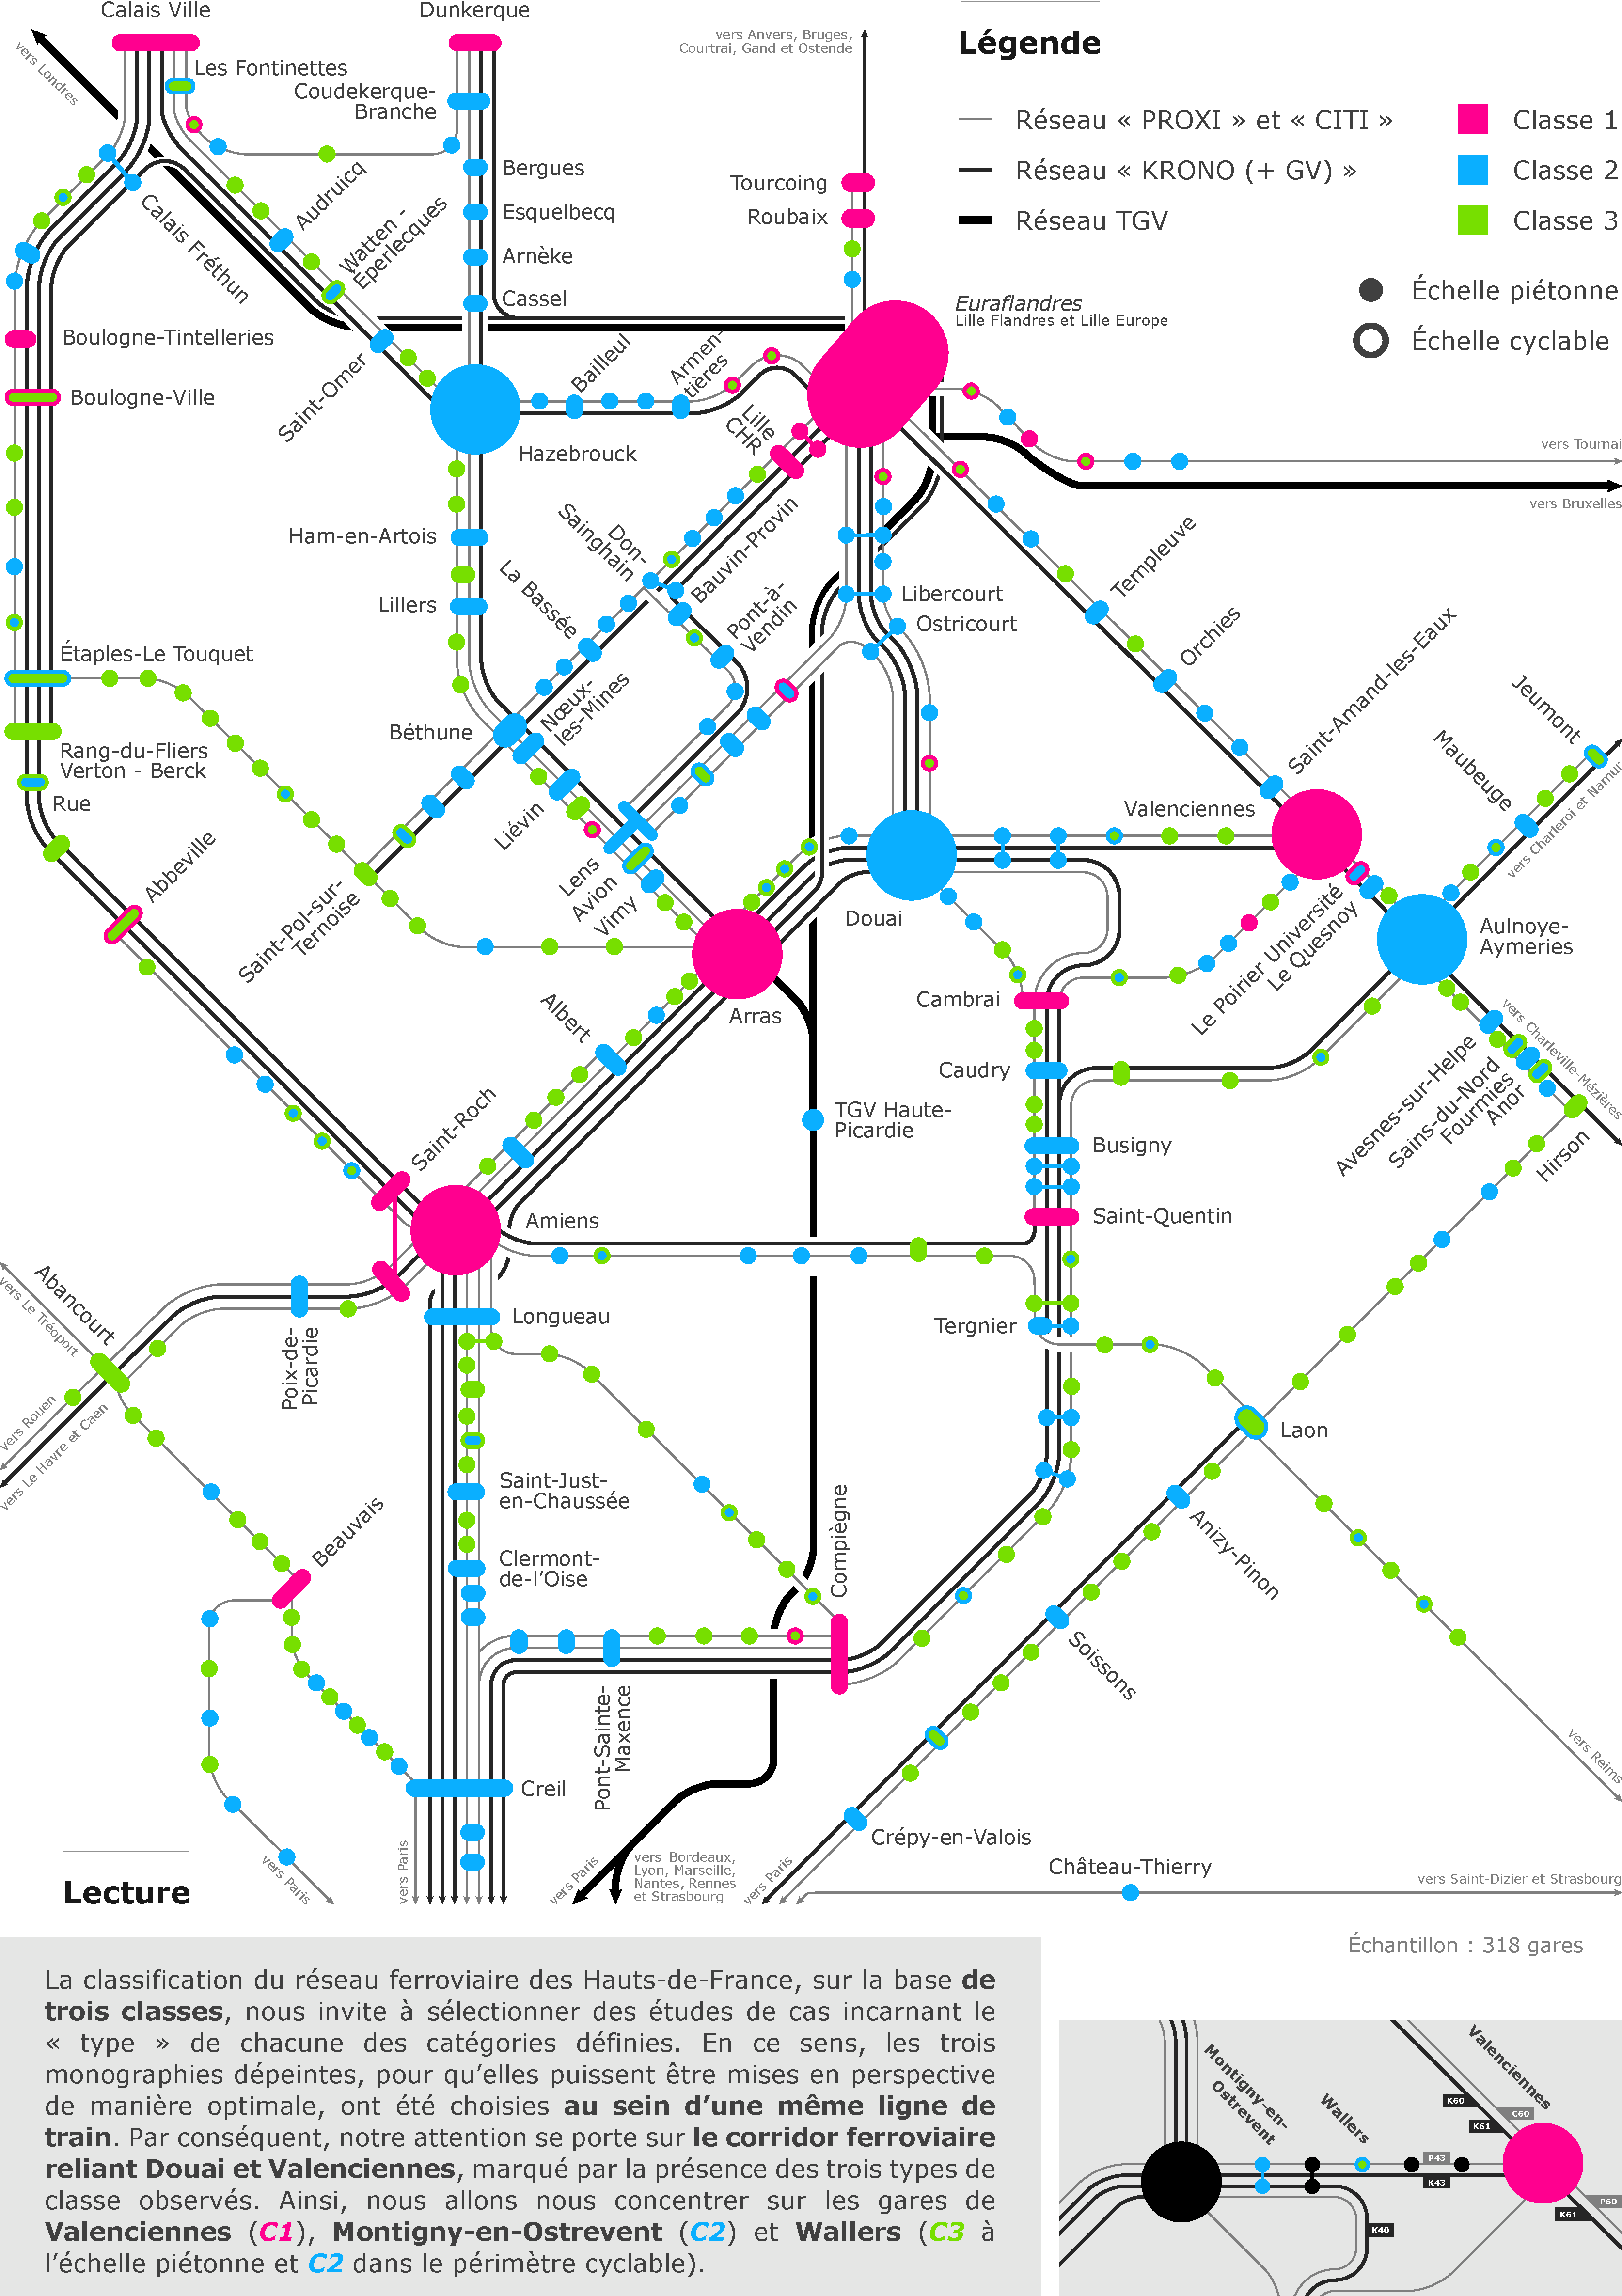
\includegraphics[width=1\columnwidth]{src/Figures/Chap-7/FR_Carte_Reseau_classification.pdf}}
        \vspace{5pt}
        \begin{flushright}\scriptsize{
        Réalisation~: \textcolor{blue}{Dylan Moinse (2024)}
        \\
        Auteur·rice·s~: projet de recherche \acrshort{NPART}
        }\end{flushright}
    \end{carte}

    % Littérature technique
Au-delà des recherches académiques sur la segmentation des gares et de leurs environs, il convient également de se référer aux rapports d’étude produits dans le cadre de notre étude de cas régionale. À l’échelle nationale, citons les travaux de \textcolor{blue}{Jean-François} \textcolor{blue}{\textcite[98-104]{troin_essai_2024}}\index{Troin, Jean-François|pagebf}, qui propose une typologie des gares françaises en cinq catégories~: les \Guillemets{gares métropolitaines}, les \Guillemets{gares spécifiques \acrshort{TGV} hors la ville}, les \Guillemets{gares de banlieue}, les \Guillemets{gares de villes moyennes} et les \Guillemets{gares rurales}. Cette catégorisation nationale, volontairement orientée sous l’angle de l’usager·ère, apporte un éclairage sur le panorama national, tout en dialoguant avec une seconde segmentation des gares exclusivement picardes. Aussi, proposons-nous de citer les rapports d’étude élaborés par \textcolor{blue}{\textcite[50-57]{hasiak_pour_2011}}\index{Hasiak, Sophie|pagebf}\index{Bodard, Géraldine|pagebf}\index{Hasiak, Fabrice|pagebf} et le \textcolor{blue}{\textcite[6]{cete_nord_picardie_profils_2011}}\index{CETE Nord Picardie@\textsl{CETE Nord Picardie}|pagebf}\index{DREAL Picardie@\textsl{DREAL Picardie}|pagebf} qui présentent différents profils de gares picardes, fondés sur un référentiel d’indicateurs comprenant les volets \Guillemets{transport/déplacements} et \Guillemets{attractivité et organisation spatiale}. Ces volets intègrent des thèmes \Guillemets{niveau de service}, \Guillemets{fréquentation}, \Guillemets{rayonnement de la gare} et \Guillemets{environnement de la gare}. La typologie des gares picardes permet de formuler à son tour cinq classes~: les \Guillemets{gares de pôles régionaux}~; les \Guillemets{gares à rayonnement francilien}~; les \Guillemets{gares de rabattement vers les pôles régionaux et Paris}~; les \Guillemets{gares de rabattement scolaire en milieu rural}~; et les \Guillemets{points d’arrêt \acrshort{TER} de petites communes}. Bien que cette répartition des gares soit utile pour dresser un portrait général, elles sont davantage descriptives que stratégiques. Sous cet angle, la classification issue du \acrshort{NPART} enrichit les connaissances existantes d’un cadre d'action plus opérationnel, en permettant de cibler les interventions publiques sur des dimensions spécifiques selon les classes.%%Rédigé%%

    % 6.4.3.3.
    \needspace{1\baselineskip} % Réserve de l'espace
\subsubsection*{Étude de cas d'un corridor ferroviaire
    \label{chap6:results-etudes-de-cas}
    }

    % Introduction
Dans une perspective résolument opérationnelle, nous avons souhaité enrichir la modélisation spatiale en intégrant une analyse qualitative fondée sur une sélection d'études de cas. À cette fin, nous avons opté pour une approche exploratoire de diagnostic territorial, largement mobilisée en aménagement du territoire pour identifier les configurations spatiales et les enjeux spécifiques à chaque site à travers une lecture sensible du terrain. Cette démarche, complémentaire à l'étude quantitative, reprend les préconisations formulées dans le rapport d'étude sur le \acrshort{NPM} en Île-de-France, publié par l'\textcolor{blue}{\textcite[5]{iau_articulation_2017}}\index{IAU@\textsl{IAU}|pagebf}. Ce document souligne la nécessité d'un diagnostic territorial afin d'éclairer et d'adapter les recommandations aux besoins contextuels des acteurs de l'aménagement.%%Rédigé%%

    % C-TOD
Dans le souci d'adopter une perspective systémique, nous avons privilégié l'étude d'un corridor ferroviaire, une approche qui offre une lecture cohérente à l'échelle d'un réseau structurant \textcolor{blue}{\autocite{bairras_slow_2025}}\index{Bairras, Philippe|pagebf}\index{Aguas Ardaiz, Iñigo|pagebf}. Cette démarche s'inscrit dans la conceptualisation du \acrfull{C-TOD}, élaborée par \textcolor{blue}{\textcite[17]{liu_conceptual_2020}}\index{Liu, Liwen|pagebf}\index{Zhang, Ming|pagebf}\index{Xu, Tao|pagebf}. Dans le cadre de notre modèle \acrshort{NPART}, nous entendons par corridor ferroviaire une liaison assurée par une ligne de \acrshort{TGV} ou de \acrshort{TER} directe, desservant chaque gare sans rupture de charge. Afin de proposer un aperçu exploratoire de ces diagnostics territoriaux, nous avons circonscrit notre analyse aux quartiers de gare effectivement accessibles en mobilité individuelle légère (\(CI\)), afin de mieux étayer notre argumentation et de démontrer la valeur ajoutée du \acrshort{NPART}. Nous avons alors délibérément restreint nos observations et nos préconisations aux outils traditionnels de l'aménagement, en envisageant une mise en œuvre à court ou à moyen terme et en excluant toute restructuration radicale du tissu bâti, considérée ici comme une donnée immuable \textcolor{blue}{\autocite[45]{stransky_periurbain_2019}}\index{Stransky, Vaclav|pagebf}.%%Rédigé%%

    % Etudes de cas
À ce titre, nous avons choisi d'étudier deux gares situées le long du corridor ferroviaire reliant Douai et Valenciennes~: Montigny-en-Ostrevent et Wallers\footnote{
    Initialement, il était prévu d'inclure également la gare de Valenciennes dans cette analyse comparative. Toutefois, pour des raisons d'économie de ressources et de faisabilité temporelle, nous avons décidé de ne pas la retenir. Cette exclusion repose sur plusieurs considérations. Premièrement, Valenciennes appartient à une catégorie de gare qui tend ou atteint déjà le modèle d'urbanisme attendu (\(C1\)), ce qui la rend moins pertinente pour notre démonstration. Deuxièmement, la classe d'appartenance de cette gare étant relativement restreinte en effectif et bien étudiée dans la littérature, son inclusion aurait apporté une plus-value limitée. Enfin, nos résultats ont démontré que le potentiel du \acrshort{M-TOD} est particulièrement significatif dans les territoires périurbains, ce qui justifie un recentrage sur Montigny-en-Ostrevent et Wallers, intégrés dans un système urbain intermédiaire.
} (voir la \hyperref[fig-chap6:schema-reseau-train-hdf-classes]{carte~\ref{fig-chap6:schema-reseau-train-hdf-classes}}, page~\pageref{fig-chap6:schema-reseau-train-hdf-classes}). Ce choix s'explique par plusieurs considérations stratégiques~:
\begin{customitemize}
    \item Tout d'abord, cette sélection repose sur une analyse des corridors ferroviaires reliant la métropole lilloise aux villes situées au sud de la capitale régionale, en s'appuyant sur les conclusions tirées de la thèse de doctorat de \textcolor{blue}{Fausto} \textcolor{blue}{\textcite[246]{lo_feudo_scenario_2014}}\index{Lo Feudo, Fausto|pagebf}\index{Menerault, Philippe|pagebf}\index{L'Hostis, Alain|pagebf}\index{Festa, Demetrio Carmine|pagebf}. Sa recherche identifie en effet des scénarios positifs de densification et d'amélioration de l'offre de transport en commun pour plusieurs villes du Bassin Minier, notamment Béthune, Lens, Douai, Somain, Bouchain et Denain. L'auteur montre \Guillemets{\textsl{clairement la possibilité d'un jeu de vases communicants dans lequel une partie de la croissance urbaine attendue dans de vastes espaces périurbains, pourrait se localiser sur les quelques espaces stratégiques identifiés dans le scénario de TOD régional.}} \textcolor{blue}{\autocite[246]{lo_feudo_scenario_2014}}\index{Lo Feudo, Fausto|pagebf}\index{Menerault, Philippe|pagebf}\index{L'Hostis, Alain|pagebf}\index{Festa, Demetrio Carmine|pagebf}~;
    \item Ensuite, nous avons opté pour une approche monographique, permettant d'illustrer chacune des classes définies dans notre typologie, hormis \(C1\), par un cas spécifique. Afin d'assurer une représentativité équilibrée, il était essentiel de sélectionner un corridor ferroviaire intégrant au moins une gare de chaque classe identifiée. Après un processus de sélection par élimination, seuls quelques corridors dans l'arc sud lillois répondaient à ces critères~;
    \item Par ailleurs, cette sélection s'inscrit dans une démarche prospective, en intégrant un corridor ferroviaire concerné par des projets structurants en matière de transport. Nous avons ainsi retenu un axe bénéficiant des transformations majeures induites par la mise en place des \acrfull{SERM} lillois, favorisant une connexion avec des études en cours, notamment celles en cours de réalisation par \textcolor{blue}{\textcite[3]{sncf_gares__connexions_connecter_2024}}\index{SNCF Gares \& Connexions@\textsl{SNCF Gares \& Connexions}|pagebf}, qui développe une méthodologie d'analyse des corridors ferroviaires à partir d'un outil de diagnostic baptisé \Guillemets{Radar}, conçu par l'agence \acrfull{AREP}. Dans leur livrable, plusieurs corridors de la région Hauts-de-France sont pris en exemple dans leurs futures études, dont celui incluant nos deux études de cas, en mettant l'accent sur quatre dimensions clés~: la capacité et la sécurité~; l'offre de services, l'accessibilité et l'intermodalité~;
    \item Une autre motivation pour ce choix repose sur la volonté de s'affranchir d'une trop forte influence de la métropole lilloise. En effet, afin d'éviter que l'analyse ne soit biaisée par la centralité du pôle d'échange \textsl{Euraflandres}, nous avons privilégié un corridor n'atteignant pas directement la \acrshort{MEL}. Cette orientation permet de mieux cerner les dynamiques propres aux territoires périurbains et aux villes moyennes, qui constituent des terrains d'expérimentation plus originaux et révélateurs des enjeux liés à l'intégration de la mobilité individuelle légère~;
    \item Enfin, une fois le corridor sélectionné, nous avons cherché à retenir des gares présentant des indicateurs proches de la médiane de leur classe d'appartenance, afin de garantir la représentativité de la classification exposée. Ce choix méthodologique vise à assurer une extrapolation pertinente des résultats et à identifier des cas illustrés dotés d'un fort potentiel d'évolution en matière d'aménagement et de mobilité soutenables.
\end{customitemize}

    % Carte Montigny-en-Ostrevent
    \begin{carte}[h!]\vspace*{4pt}
        \caption{Diagnostic territorial du quartier de gare étendu de Montigny-en-Ostrevent.}
        \label{fig-chap6:monographie-montigny}
        \centerline{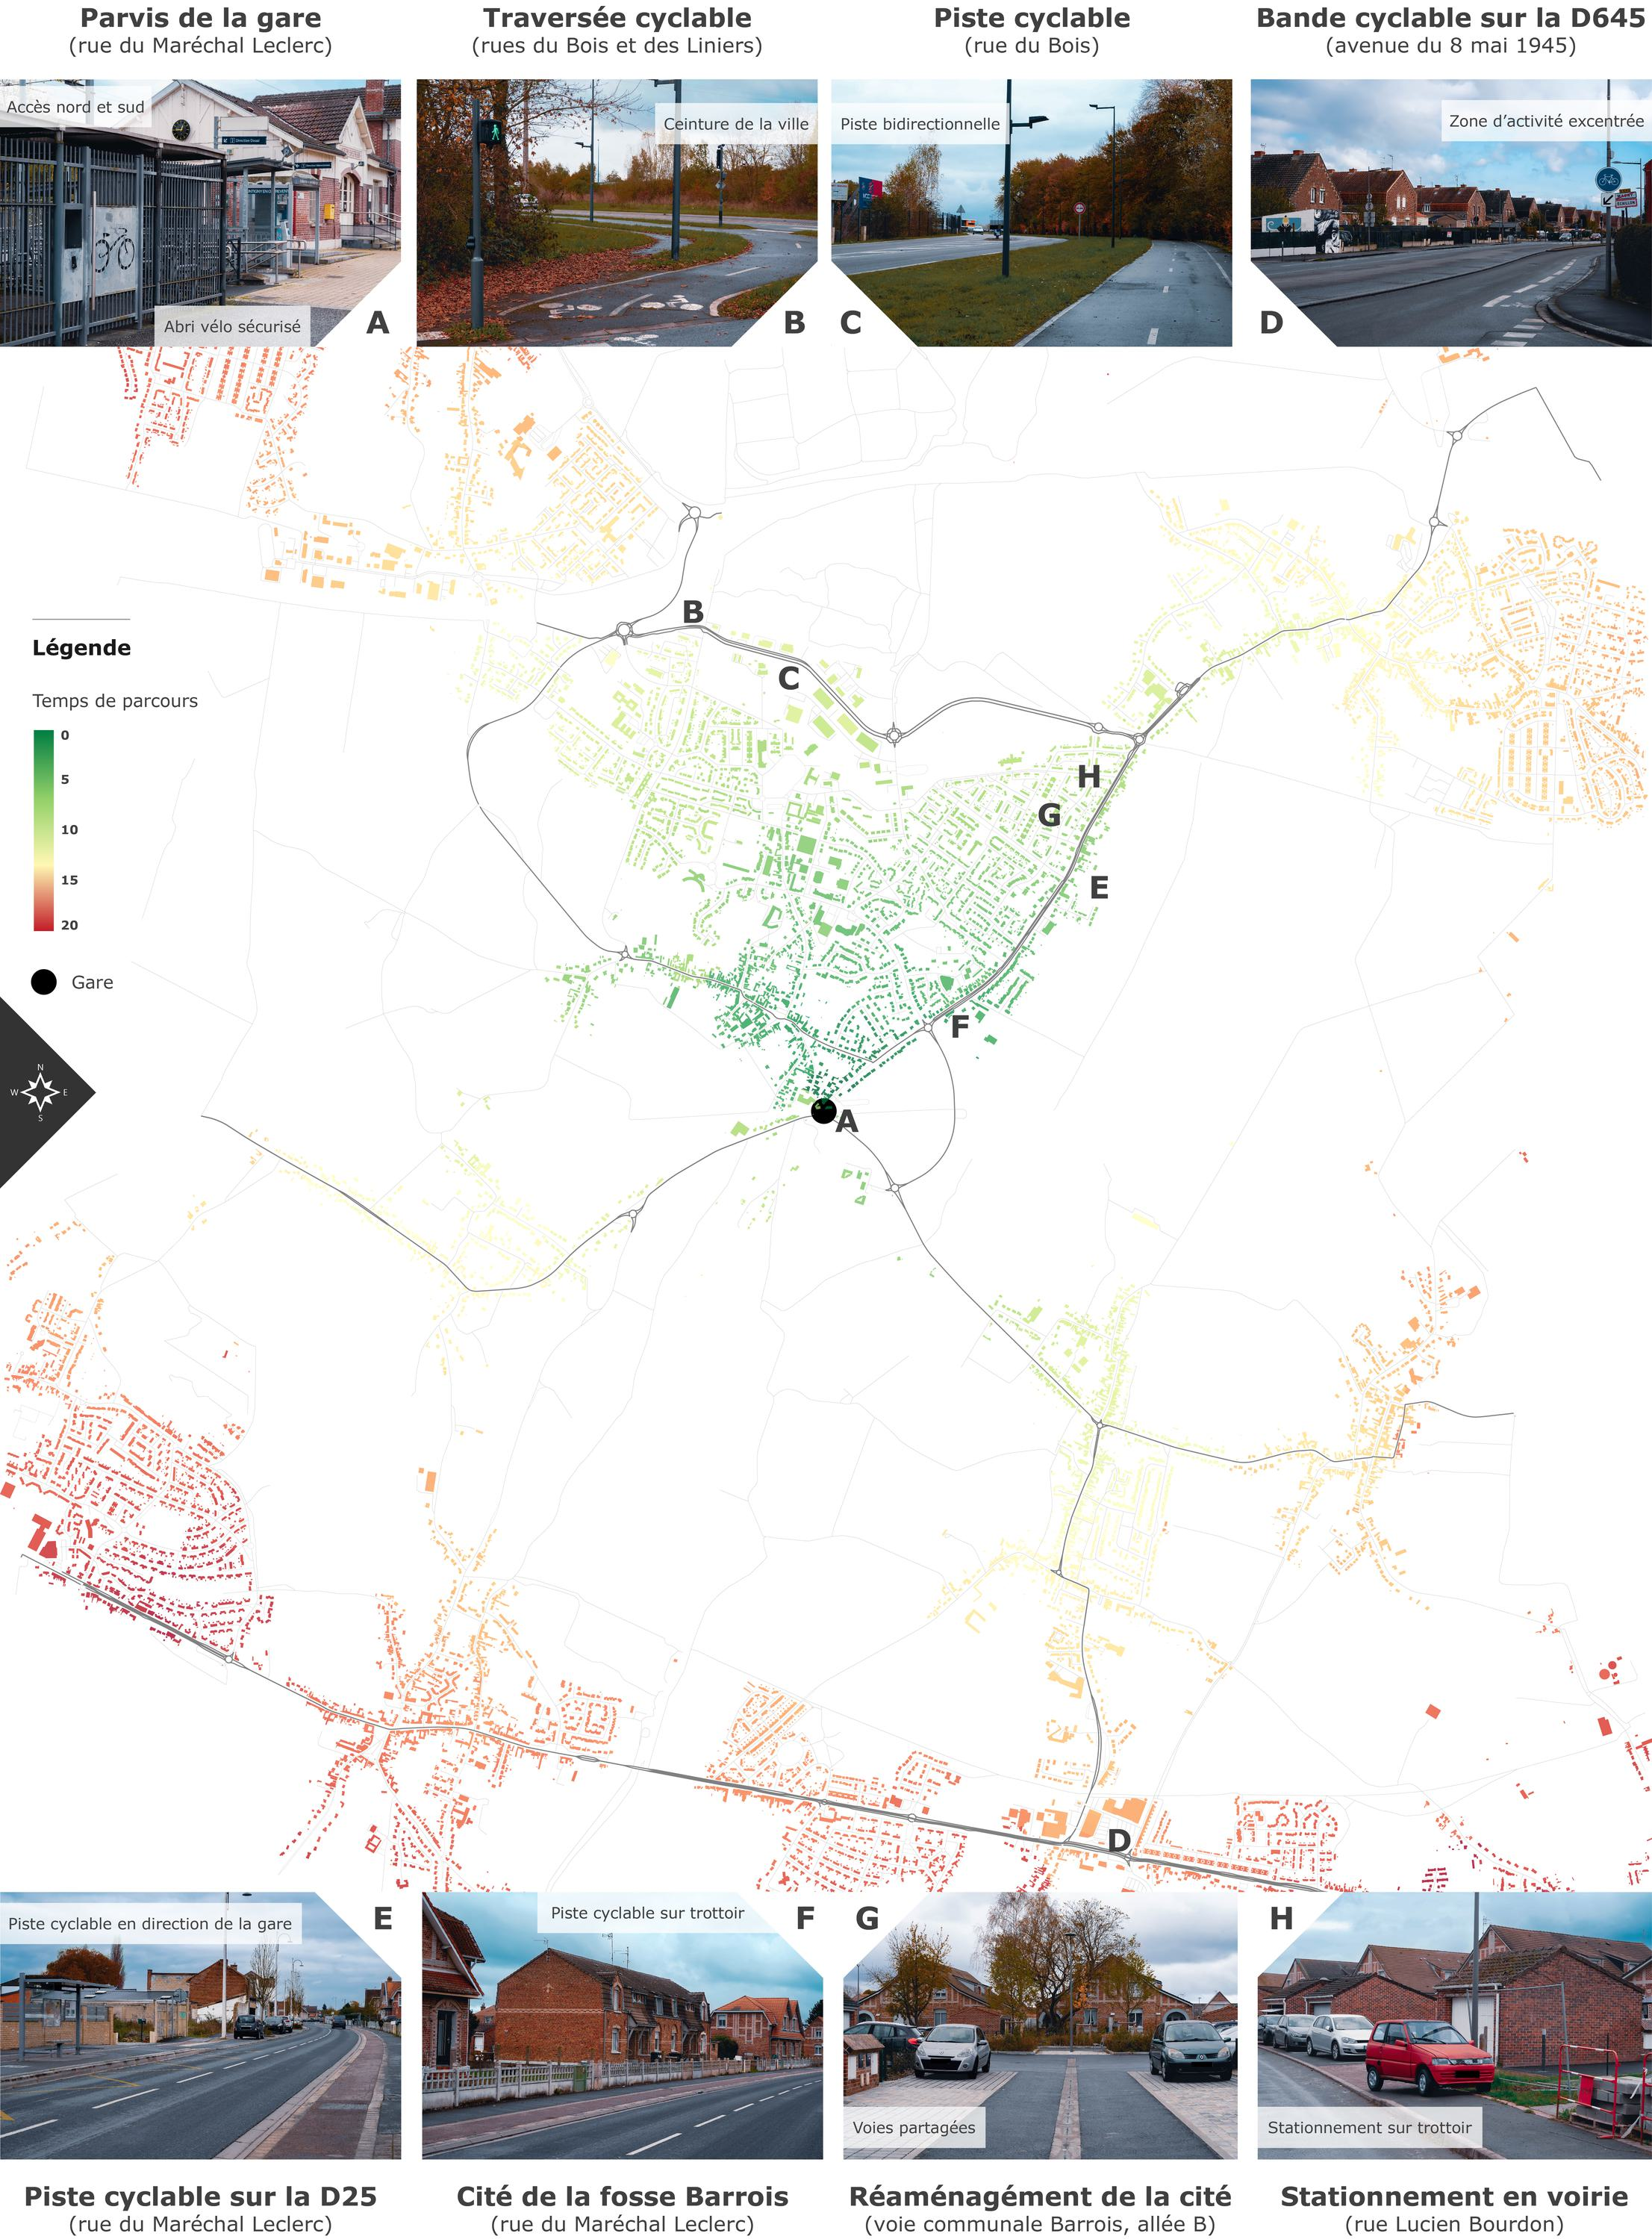
\includegraphics[width=1\columnwidth]{src/Figures/Chap-6/FR_NPART_Montigny.jpg}}
        \vspace{5pt}
        \begin{flushright}\scriptsize{
        Réalisation~: \textcolor{blue}{Dylan Moinse (2025)}
        \\
        Photographies (A), (B), (C), (D), (E), (F), (G) et (H)~: \textcolor{blue}{Dylan Moinse (2024)}
        \\
        Auteur·rice·s~: projet de recherche \acrshort{NPART}
        }\end{flushright}
    \end{carte}

    % Présentation Montigny-en-Ostrevent
La gare de Montigny-en-Ostrevent constitue un cas d'étude particulièrement intéressant, inscrite dans l'agglomération de Douai et à proximité de la ville de Somain. La commune compte environ 5~000 habitant·e·s, avec une démographie en léger déclin depuis les années 1960. La gare est desservie par la ligne ferroviaire reliant Douai à Valenciennes (P43) ainsi que par une liaison directe entre Lille Flandres et Saint-Quentin (K40), lui conférant une connexion régionale relativement performante. En revanche, le \acrshort{TERGV} de la ligne K43, reliant Arras à Valenciennes en passant par Douai, ne s'y arrête pas. Dotée d'un bâtiment voyageurs avec guichet et automate, elle dispose également d'un espace de stationnement automobile et d'un abri vélo sécurisé à proximité directe, et est desservie par les lignes 3~; 12 et 108 du réseau de bus douaisien \textsl{Évéole}. Au regard des critères d'analyse retenus et de l'interprétation des classes dans le \acrshort{NPART}, cette gare et ses environs présentent les caractéristiques apparentes d'un \acrshort{TAD} et se classent dans \(C2\), aussi bien à l'échelle piétonne qu'à l'échelle cyclable (voir la \hyperref[fig-chap6:monographie-montigny]{carte~\ref{fig-chap6:monographie-montigny}}, page~\pageref{fig-chap6:monographie-montigny}).%%Rédigé%%

    % Diagnostic territorial Montigny-en-Ostrevent - Node
La gare enregistre une fréquentation annuelle d'environ 130~000 voyageur·se·s, soit 60~\% de moins que la moyenne régionale (\(RT\)). En ce qui concerne l'offre ferroviaire, la gare de Montigny-en-Ostrevent bénéficie d'une fréquence relativement élevée, supérieure de 38~\% à la moyenne (\(N_{3}\), 44 \acrshort{TER})~; et d'une amplitude horaire élargie, supérieure de 7~\% en semaine et de 16~\% le week-end (\(N_{5}\) et \(N_{6}\), respectivement 16 et 15 heures). Son réseau dispose également d'un niveau de degré de proximité accru de 35~\% (\(N_{10}\)), ce qui appuie sa position stratégique au sein d'une conurbation urbaine mise en réseau. De surcroît, la gare profite d'un accès facilité au centre de Lille, avec un temps de trajet en train inférieur de 29~\% et nécessitant 28~\% d'arrêts en moins pour atteindre la métropole régionale (\(N_{14}\)et \(N_{15}\), en 30 minutes et en 1 arrêt).%%Rédigé%%

    % Diagnostic territorial Montigny-en-Ostrevent - Place
Toutefois, ces atouts en matière de desserte ferroviaire sont contrebalancées par un développement urbain et une connectivité locale moins favorables. Bien que la densité de population dans l'aire d'influence cyclable de la gare Montigny-en-Ostrevent soit comparable à la moyenne régionale, la densité d'emploi y est inférieure de 44~\% (\(P_{2}\), 107 emplois par kilomètre carré), certainement en partie en raison d'un taux d'occupation du sol consacré aux activités de bureau et industrielles inférieur de 70~\% à la moyenne (\(P_{5}\), 1,2~\%). En conséquence, la gare pâtit d'une offre de service limitée, les équipements étant 23~\% moins nombreux pour les \acrshort{POIs} dits de \Guillemets{proximité}, 39~\% pour ceux de gamme \Guillemets{intermédiaire}, et 66~\% pour ceux de catégorie \Guillemets{supérieure} (\(P_{7}\), \(P_{8}\) et \(P_{9}\)). Néanmoins, le quartier de gare cyclable se distingue par une proportion importante de logements sociaux, plus de deux fois supérieure à la moyenne régionale (\(P_{12}\), 16~\%).%%Rédigé%%

    % Diagnostic territorial Montigny-en-Ostrevent - Accessibility
En ce qui concerne le traitement des espaces publics, les infrastructures piétonnes sont relativement bien développées, avec une densité d'infrastructure piétonne supérieure de 18~\% à la moyenne des gares (\(A_{1}\), 86 kilomètres). Plus notable encore, la densité du réseau cyclable y est particulièrement élevée, supérieure de 188~\% à la moyenne (\(A_{4}\), 9 kilomètres), offrant ainsi un potentiel favorable à l'essor de la mobilité individuelle légère. De plus, les habitant·e·s de Montigny-en-Ostrevent présentent un taux de motorisation inférieur de 62~\% (\(A_{11}\), 76~\%). En revanche, plusieurs limitations sont à relever. L'offre de stationnement vélo demeure insuffisante, malgré la présence d'un abri vélo en gare, avec un nombre de places inférieure de 57~\% à la moyenne régionale (\(A_{5}\), 53 places). De plus, l'efficacité spatiale de l'isochrone cyclable~–~c'est-à-dire la surface réellement accessible par rapport à son rayonnement supposé~–~est inférieure de 46~\% (\(A_{3}\), 18~\%). Nos observations de terrain confirment qu'en dépit d'un réseau cyclable relativement dense, celui-ci est fragmenté et limité à certains tronçons de départementales, souvent aménagés sous forme de bandes cyclables ou de pistes étroites et peu confortables. Un dernier point critique réside dans la place encore prépondérante accordée à l'automobile, aussi bien dans l'organisation du tissu urbain que dans la répartition des infrastructures de transport. Cela peut donner lieu à des réflexions sur la nécessité d'accompagner les interventions d'urbanisme ferroviaire et cyclable par des actions de modération de la circulation et de réduction de la capacité routière. Il convient à cet effet d'éviter un phénomène de \Guillemets{vases communicants}, où l'amélioration des infrastructures piétonnes et cyclables pourrait être en partie neutralisée par le maintien d'un réseau routier favorisant encore trop largement la voiture \textcolor{blue}{\autocite[259]{lo_feudo_scenario_2014}}\index{Lo Feudo, Fausto|pagebf}\index{Menerault, Philippe|pagebf}\index{L'Hostis, Alain|pagebf}\index{Festa, Demetrio Carmine|pagebf}.%%Rédigé%%

    % Carte Wallers
    \begin{carte}[h!]\vspace*{4pt}
        \caption{Diagnostic territorial du quartier de gare étendu de Wallers.}
        \label{fig-chap6:monographie-wallers}
        \centerline{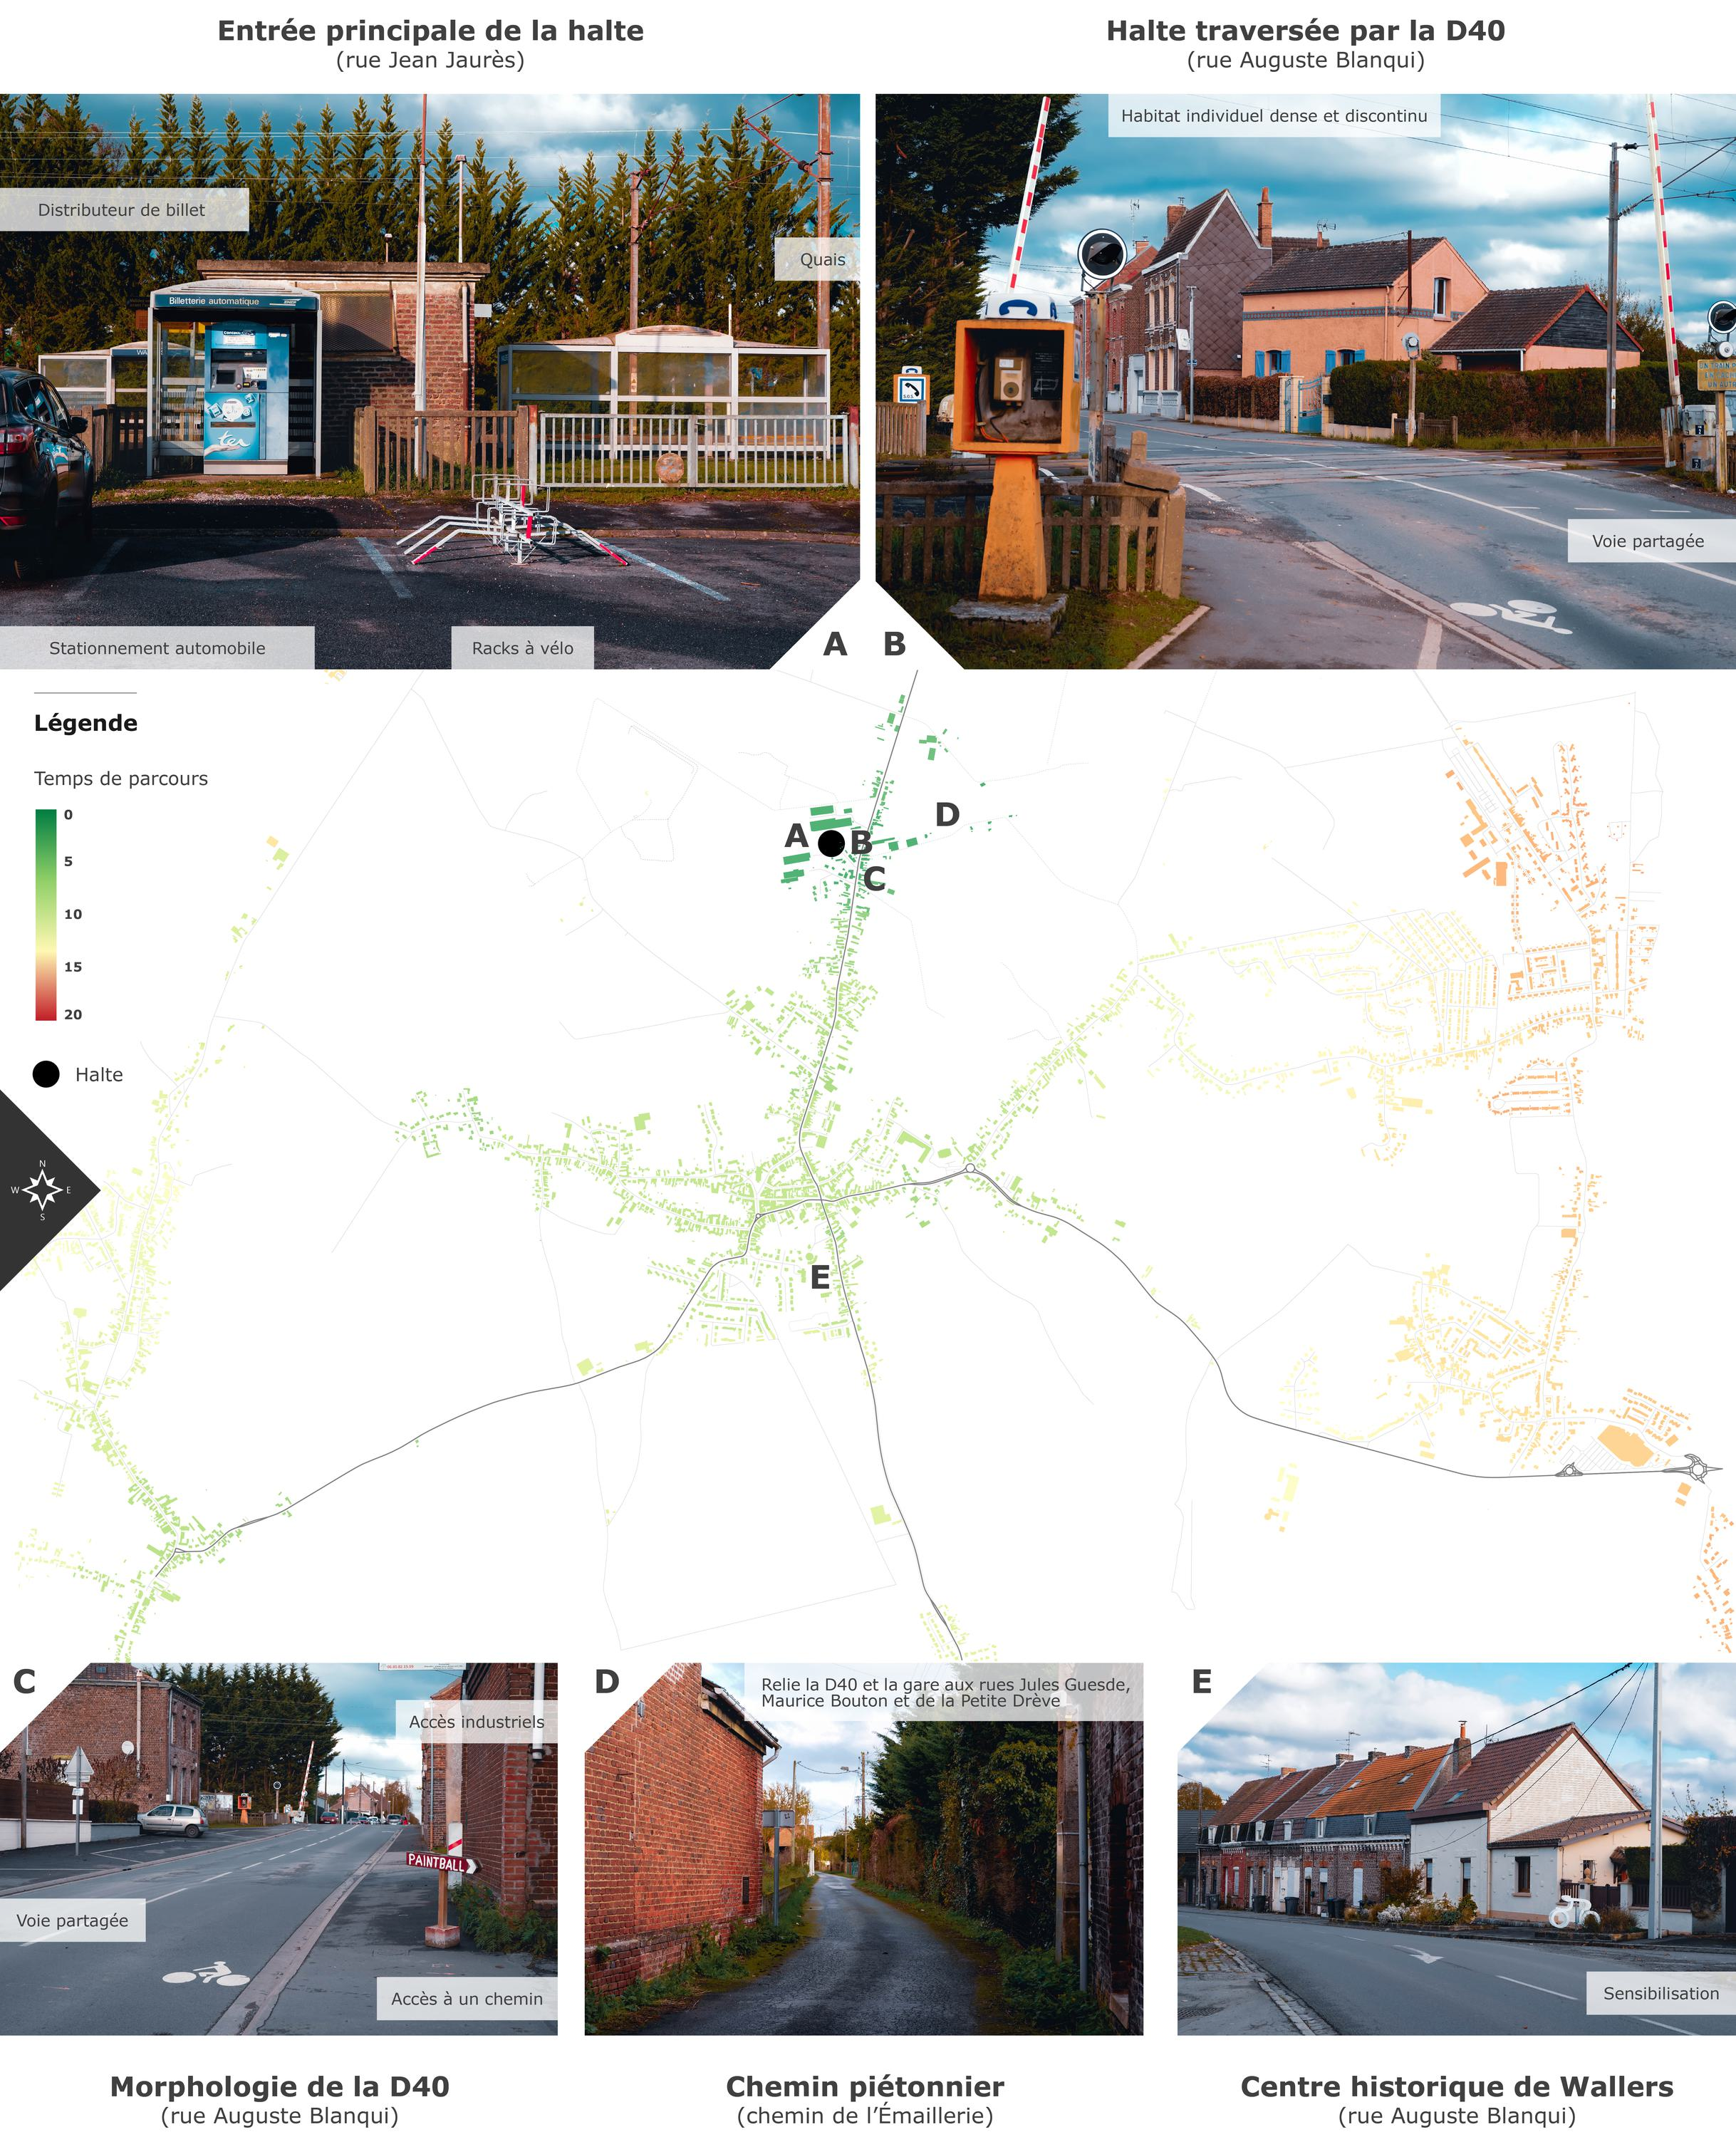
\includegraphics[width=1\columnwidth]{src/Figures/Chap-6/FR_NPART_Wallers.jpg}}
        \vspace{5pt}
        \begin{flushright}\scriptsize{
        Réalisation~: \textcolor{blue}{Dylan Moinse (2025)}
        \\
        Photographies (A), (B), (C), (D), et (E)~: \textcolor{blue}{Dylan Moinse (2024)}
        \\
        Auteur·rice·s~: projet de recherche \acrshort{NPART}
        }\end{flushright}
    \end{carte}

    % Présentation Wallers
La halte de Wallers constitue notre seconde étude de cas qui nous a semblé intéressante, en raison de son insertion urbaine complexe due à sa position excentrée par rapport au tissu urbain historique de la commune (voir la \hyperref[fig-chap6:monographie-wallers]{carte~\ref{fig-chap6:monographie-wallers}}, page~\pageref{fig-chap6:monographie-wallers}). Dans le cadre du \acrshort{NPART}, cette halte apparaît en situation de \Guillemets{dépendance}, tant à l'échelle piétonne que cyclable, en raison de son faible degré d'intégration avec le tissu urbain. Cette halte ferroviaire est exclusivement desservie par une départementale qui coupe la voie ferrée, ce qui en fait un espace peu intégré aux dynamiques urbaines locales. Comme le souligne le précédent \acrfull{PDU} 2013-2023 du \textcolor{blue}{\textcite[78]{siturv_plan_2014}}\index{SITURV@\textsl{SITURV}|pagebf}, bien que la halte soit située sur la dorsale minière et bénéficie d'une offre ferroviaire relativement soutenue, son isolement par rapport aux centralités urbaines nuit à son attractivité. Cette situation explique son classement dans la dernière catégorie (\(C3\)) à l'échelle piétonne (\(PI\)). À l'inverse, à l'échelle cyclable (\(CI\)), la halte est davantage connectée, pouvant être rejointe depuis le centre urbain de Wallers ainsi que depuis certaines communes limitrophes. Dès lors, au niveau cyclable, le quartier de halte de Wallers rejoint la deuxième classe (\(C2\)). Cette extension du quartier de halte de Wallers permettant de la connecter à l'urbain suit non seulement la départementale, mais aussi un réseau viaire secondaire, constitué de chemins, exclusivement accessibles aux mobilités actives ou aux riverain·e·s. Située en périphérie de l'agglomération valenciennoise, Wallers est une commune d'environ 6~000 habitant·e·s, dont la démographie a connu un déclin continu depuis les années 1950 avant de se stabiliser dans les années 2000. Seule la ligne P43 reliant Douai à Valenciennes marque l'arrêt à Wallers. La halte est par ailleurs desservie par les lignes 107 et 110 du réseau de bus valenciennois \textsl{Transville}.%%Rédigé%%

    % Diagnostic territorial Wallers - Node
La fréquentation annuelle de la gare de Wallers est très limitée, avec 11~000 voyageur·se·s, soit seulement 3~\% de la fréquentation moyenne des gares régionales (\(RT\)). Cette situation peut être attribuée à plusieurs facteurs explicatifs, notamment un niveau de service perfectible en premier lieu. La fréquence quotidienne des trains est inférieure de 29~\% à la moyenne (\(N_{3}\), 22 \acrshort{TER}), et le degré de proximité de la gare est légèrement réduite, avec un niveau inférieur de 10~\% (\(N_{10}\)). Toutefois, certains indicateurs présentent des résultats plus nuancés. La gare dispose d'une amplitude horaire supérieure à la moyenne, avec une plage horaire élargie de 7~\% en semaine et de 12~\% le week-end (\(N_{5}\) et \(N_{6}\), respectivement 16 et 14 heures). De plus, malgré le besoin d'effectuer une correspondance à Valenciennes ou à Douai, le temps de trajet jusqu'à Lille demeure relativement viable, avec une durée moindre de 22~\% (\(N_{14}\), 50 minutes) et un nombre d'arrêts intermédiaires réduit de 17~\% (\(N_{13}\), 3 arrêts). En termes d'aménagement, la gare se présente sous la forme d'une halte ferroviaire rudimentaire, marquée par l'absence de véritable pôle intermodal. Elle comprend un ancien bâtiment voyageur aujourd'hui inoccupé et un automate. Du point de vue des infrastructures de stationnement, elle dispose uniquement d'un espace réservé aux véhicules motorisés et de racks à vélo non surveillés.%%Rédigé%%

    % Diagnostic territorial Wallers - Place
Toutefois, ce qui freine le plus l'attractivité de la halte de Wallers réside dans les faibles degrés de développement urbain et de \textsl{design}. En dépit du potentiel d'extension de son aire d'influence grâce à la mobilité individuelle légère, la gare ne permet de rejoindre qu'une concentration urbaine peu dense, où la densité de population est inférieure de 38~\% à la moyenne des gares de la région (\(P_{1}\), 834 habitant·e·s par kilomètre carré). Plus encore, sa densité d'emploi est 56~\% inférieure (\(P_{2}\), 86 emplois par kilomètre carré), traduisant une forme de spécialisation résidentielle marquée de son quartier de gare cyclable. Cet usage des sols à dominante résidentielle peut être vu au travers du taux d'occupation des activités industrielles, inférieur de 61~\%, et des espaces verts, inférieur de 78~\% par rapport aux autres gares (\(P_{5}\) et \(P_{6}\), respectivement 1,6~\% 0,3~\% de l'usage des sols). Nous pouvons également y constater une rareté des \acrshort{POIs}, dont la présence est inférieure de 51~\% à 90~\% selon les gammes considérées  (\(P_{7}\), \(P_{8}\) et \(P_{9}\)), ainsi qu'une valeur foncière des activités inférieure de 95~\% à la moyenne régionale (\(P_{11}\), 100~\euro~par mètre carré).%%Rédigé%%

    % Diagnostic territorial Wallers - Design
Au regard de la qualité de ses espaces publics, la halte de Wallers souffre d'un manque de connectivité. Le réseau piéton est peu développé, avec une longueur d'espaces piétonniers inférieure de 33~\% à la moyenne (\(A_{1}\), 48 kilomètres). Un autre défi de taille est l'offre d'infrastructures cyclables qui y est déficitaire, avec une longueur moindre de 75~\% (\(A_{4}\), 1 kilomètre). Plus généralement, le réseau de voirie est peu maillé, avec 61~\% d'intersections en moins par rapport aux autres quartiers de gare (\(A_{2}\), 51 par kilomètre carré). L'insuffisance des infrastructures dédiées au vélo constitue alors un frein majeur~: notons que seules 16 places de stationnement vélo y sont disponibles, soit 87~\% de moins que la moyenne de notre échantillon de gares (\(A_{5}\)). Cette carence nuit directement à l'attractivité du train comme alternative à l'automobile. Néanmoins, certains éléments encourageants ressortent de ce diagnostic exploratoire~: les ménages résidant dans les territoires rendus accessibles sont relativement moins motorisés, avec un taux d'équipement inférieur de 20~\% (\(A_{11}\), 68~\%). Cette caractéristique souligne un potentiel sous-exploité, qui pourrait être mobilisé afin d'encourager une reconfiguration du quartier de gare autour de la marche et de la mobilité individuelle légère, adaptée à une population peu motorisée.%%Rédigé%%

    % ___________________________________________
    % 6.*.
    \newpage
    \needspace{1\baselineskip} % Réserve de l'espace
    \addcontentsline{toc}{section}{Conclusion du chapitre~6}
    \sectionheader{Conclusion du chapitre}
\section*{Conclusion du chapitre~6
    \label{chap6:conclusion}
    }
    %\markright{Conclusion du chapitre~6}{}

    % Intérêt du NPART
Développer des quartiers de gare requiert fréquemment de privilégier un aspect ou un critère au détriment d’autres, soulevant ainsi des débats internationaux sur le \acrshort{TOD} quant à la possibilité d’optimiser simultanément un nombre important de paramètres \textcolor{blue}{\autocite[181]{veloso_e_zarate_quartiers_2024}}\index{Veloso e Zarate, Halina|pagebf}\index{Triggianese, Manuela|pagebf}\index{Baron, Nacima|pagebf}\index{Le Bot, Nils|pagebf}\index{Detavernier, Pauline|pagebf}. Dans cette perspective, il est essentiel de cerner les leviers d’action et leurs effets pour encourager un développement orienté vers le rail et soutenu par la mobilité individuelle légère, dans un contexte où émergent des formes spécialisées de \acrshort{TOD} \textcolor{blue}{\autocite[111]{cervero_transit-oriented_2017}}\index{Cervero, Robert|pagebf}\index{Guerra, Erick|pagebf}\index{Al, Stefan|pagebf}. C’est dans ce cadre que nous avons élaboré le modèle \acrshort{NPART}, conçu pour identifier et mieux comprendre les mécanismes favorisant le développement du \acrshort{M-TOD}.%%Rédigé%%

    % Figure Screen GitHub 1
    \begin{figure}[h!]\vspace*{4pt}
        \caption{Capture d’écran de la page d’accueil du dépôt \Marque{GitHub}.}
        \label{fig-chap6:screen-github-1}
        \centerline{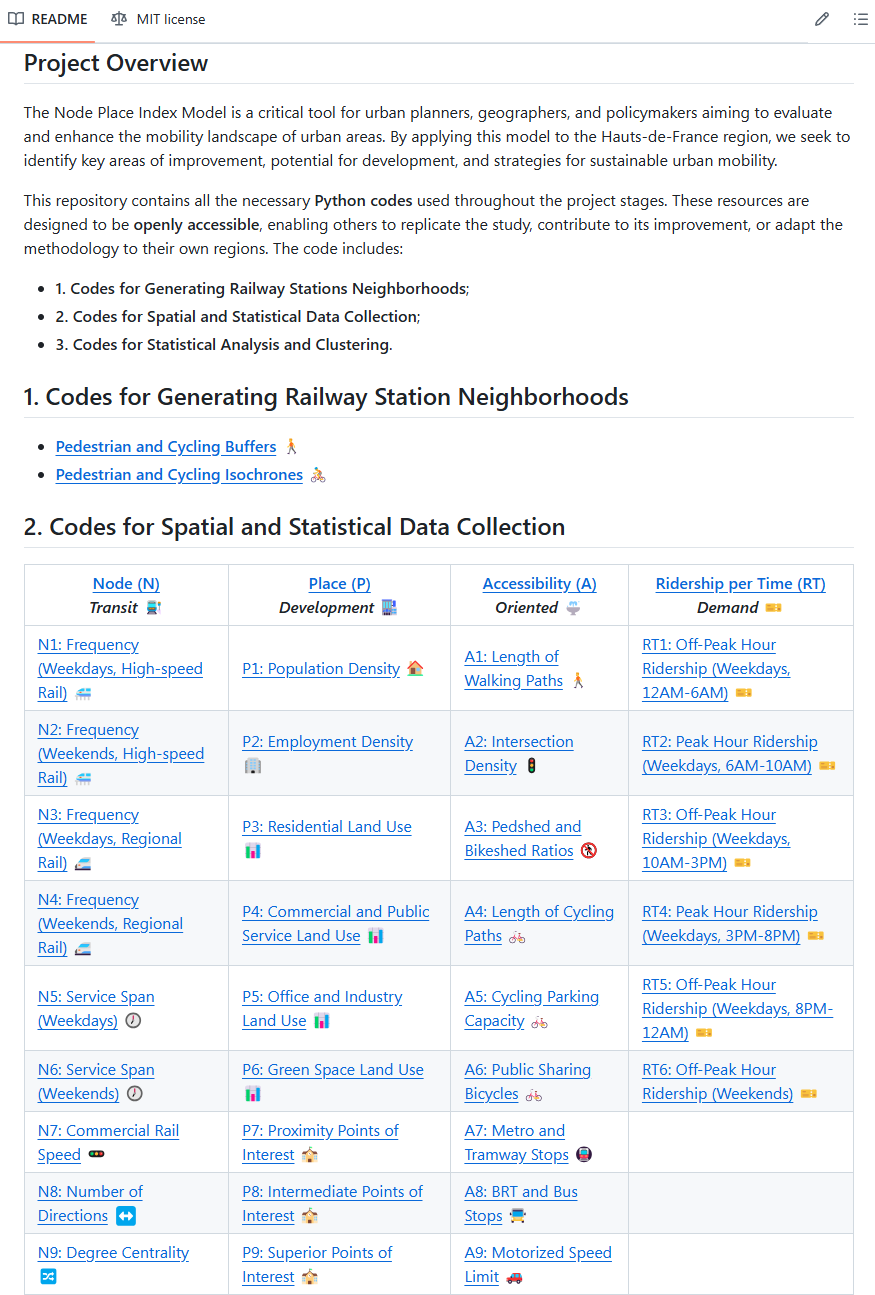
\includegraphics[width=1\columnwidth]{src/Figures/Chap-6/FR_EN_NPART_Screen_Github_1.png}}
        \vspace{5pt}
        \begin{flushright}\scriptsize{
        Réalisation~: \textcolor{blue}{Dylan Moinse (2024)}
        \\
        Auteur·rice·s~: projet de recherche \acrshort{NPART}
        }\end{flushright}
    \end{figure}

    % Figure Screen GitHub 2
    \begin{figure}[h!]\vspace*{4pt}
        \caption{Extrait d'un tutoriel en langage \textsl{Python}, formaté en \textsl{Markdown} et mis à disposition sur \Marque{GitHub}.}
        \label{fig-chap6:screen-github-2}
        \centerline{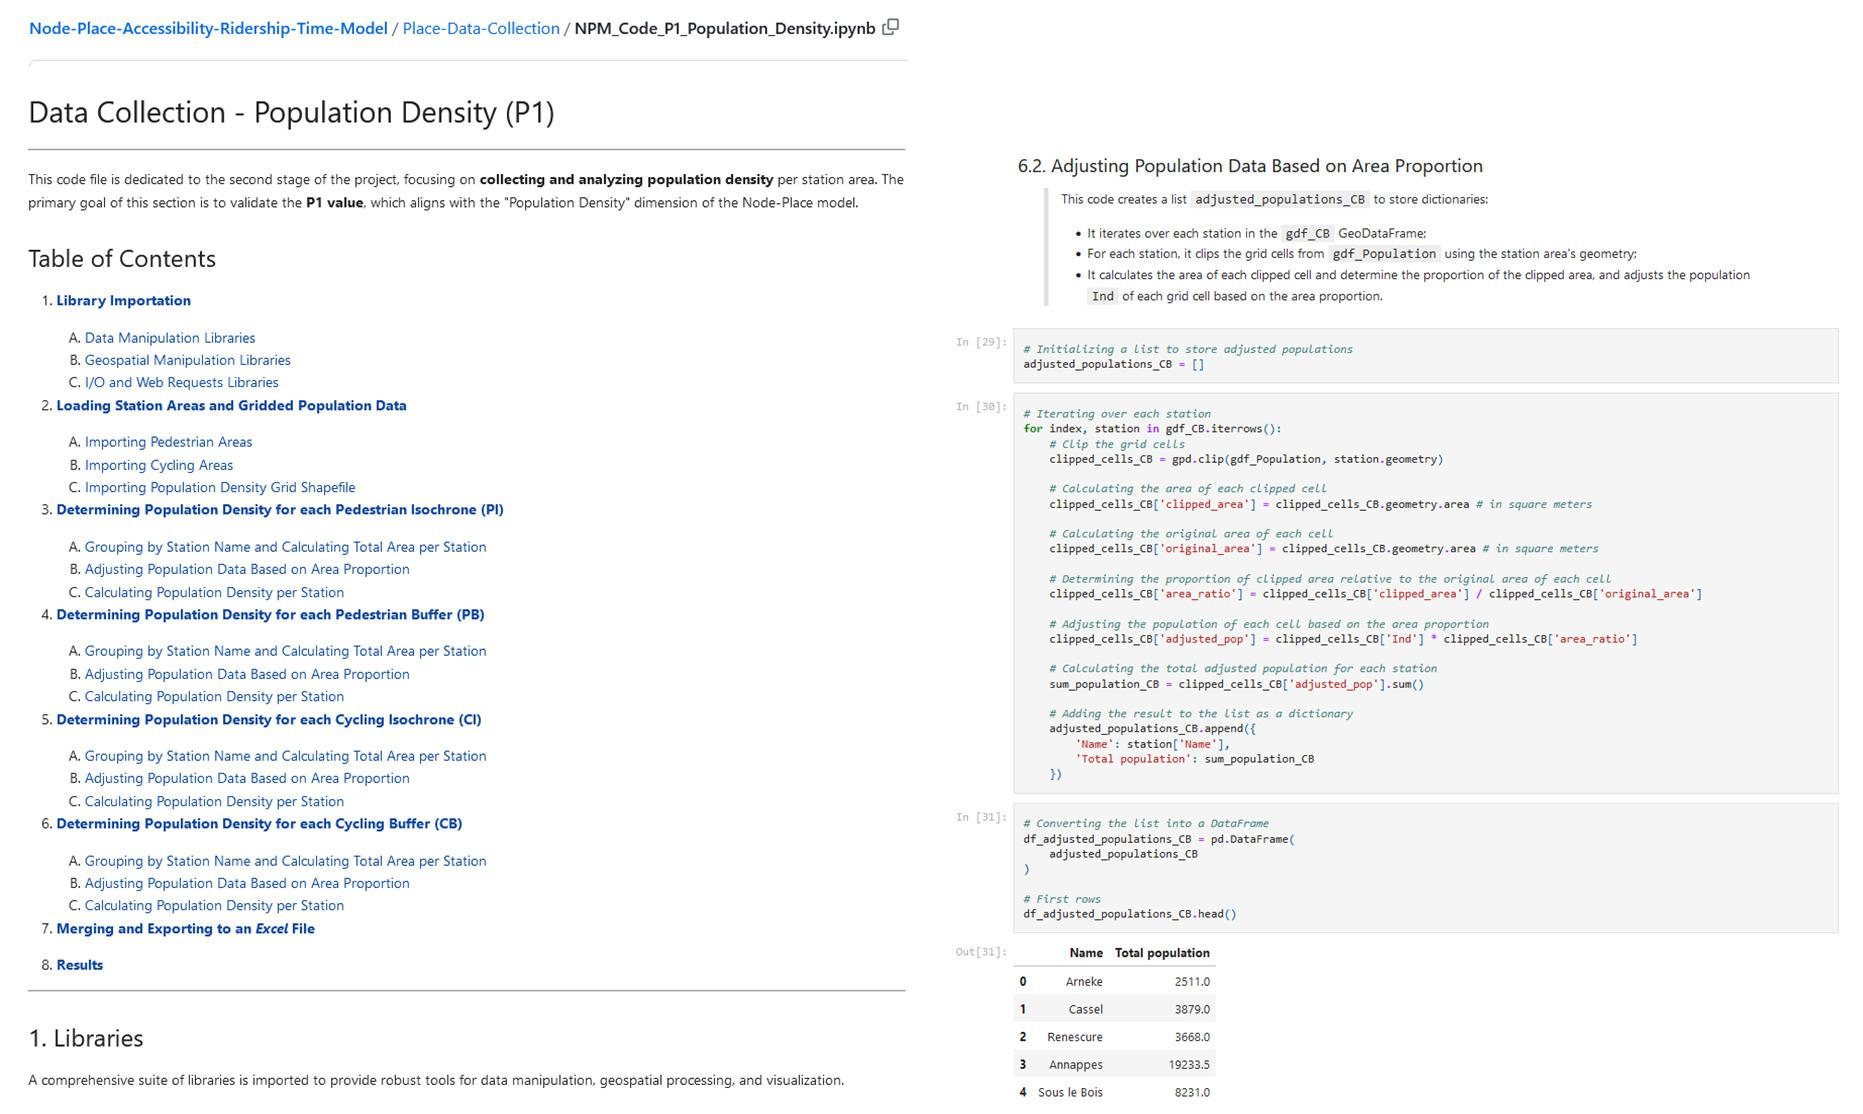
\includegraphics[width=1\columnwidth]{src/Figures/Chap-6/FR_EN_NPART_Screen_Github_2.jpeg}}
        \vspace{5pt}
        \begin{flushright}\scriptsize{
        Réalisation~: \textcolor{blue}{Dylan Moinse (2024)}
        \\
        Auteur·rice·s~: projet de recherche \acrshort{NPART}
        }\end{flushright}
    \end{figure}

    % 6.*.*
    \needspace{1\baselineskip} % Réserve de l'espace
\subsection*{Principaux enseignements
    \label{chap6:principaux-enseignements}
    }

    % Classification
La classification des gares et de leurs aires d'influence a permis de dégager trois classes distinctes, précisant ainsi le portrait général du réseau ferroviaire, caractérisé par une majorité de gares dites \Guillemets{dépendantes}, aussi bien à l’échelle piétonne que cyclable. Seules 6~\% des gares s’inscrivent dans la classe correspondant au \acrshort{TOD}, tandis que près de la moitié du réseau appartient à la catégorie des gares au potentiel \acrshort{TOD}. Notons que la proportion de gares relevant de la première classe, considérée comme l’aboutissement vers le modèle d’aménagement urbain, double lorsque les quartiers de gare sont élargis. Cela souligne l’importance de promouvoir des solutions adaptées aux \Guillemets{premiers et derniers kilomètres}, telles que la mobilité individuelle légère. Par ailleurs, l’amélioration du \textsl{design}, à laquelle le vélo contribue de manière significative, se révèle positivement corrélée aux autres dimensions du modèle. Ces liens d'interdépendance mettent en avant le rôle stratégique des connexions entre la qualité de service ferroviaire et le degré de développement urbain, confirmant ainsi l’intérêt d’une approche intégrée pour renforcer l’attractivité et la fonctionnalité des territoires desservis.%%Rédigé%%

    % Critères M-TOD
Au travers de cette modélisation, nous avons eu l'occasion de mieux définir et situer l’impact des principaux critères contribuant à la définition d’un \acrshort{TOD} basée sur une portée étendue de la marche combinée et d’un \acrshort{M-TOD}. Du côté de l’infrastructure et du service de transport en commun, tant à l’échelle piétonne qu’à l’échelle cyclable, des facteurs tels que la fréquence du service ferroviaire, la centralité de proximité, le degré de centralité, le nombre de directions et le nombre de stations accessibles en une heure se révèlent déterminants pour accroître la fréquentation en gare. En ce qui concerne l’intensité des activités, des critères tels que la valeur foncière des activités industrielles, commerciales et de bureau, les \acrshort{POIs} \Guillemets{supérieurs} et \Guillemets{intermédiaires}, ainsi que la présence d’espaces verts, figurent parmi les composantes principales. Cependant, à l’échelle cyclable, la densité d’emploi s’affirme comme un facteur encore plus prépondérant, se positionnant en tête des indicateurs clés. Enfin, pour ce qui est de la connectivité locale, la desserte en métro et en tramway, ainsi que les éléments favorisant l’hospitalité territoriale à l’égard du développement du vélo~–~tels que la présence de \acrshort{VLS}, de stationnement et d'aménagements cyclables~–~s’imposent comme les facteurs les plus influents pour les deux échelles géographiques. Ce panorama des principaux indicateurs définissant cette stratégie urbaine revisitée met également en lumière un certain décalage par rapport aux objectifs fixés par les aménageur·se·s français·es. Ces dernier·ère·s privilégient en effet davantage l’accès aux centralités urbaines, telles qu’Euralille et Châtelet, la spécialisation commerciale des territoires, le développement du réseau piéton, ainsi que la limitation de la vitesse motorisée et de la possession automobile.%%Rédigé%%

    % 6.*.*
    \needspace{1\baselineskip} % Réserve de l'espace
\subsection*{Valorisation du \acrshort{NPART}
    \label{chap6:conclusion-valorisation}
    }

    % GitHub
Dans une démarche visant à assurer la reproductibilité du modèle, nous avons veillé à rendre le processus de collecte et d’analyse des données entièrement transparent en le diffusant via une page \Marque{GitHub}\footnote{
    \Marque{GitHub}~(\url{https://github.com/}) est une plateforme en ligne de gestion de développement de logiciels et un service d'hébergement des projets en libre accès.
} (voir la \hyperref[fig-chap6:screen-github-1]{capture d'écran~\ref{fig-chap6:screen-github-1}}, page~\pageref{fig-chap6:screen-github-1}). Ce choix s’inscrit également dans une logique d’automatisation et d’applicabilité améliorée du modèle, rendues possibles par l’utilisation exclusive du langage \textsl{Python}. Ce dernier facilite non seulement l’exécution automatique du modèle, mais également son adaptation à d’autres contextes géographiques et temporels.  Ainsi, la publication en ligne dans un environnement accessible à une vaste communauté de développeur·se·s offre de nouvelles perspectives pour le modèle en tant qu’outil évolutif, permettant à la communauté scientifique et aux praticien·ne·s d’explorer des voies d’amélioration. À cette fin, le code a été systématiquement rédigé sous forme de tutoriel (voir l'\hyperref[fig-chap6:screen-github-2]{extrait de code sur la détermination de la densité de population (\(P_{1}\))~\ref{fig-chap6:screen-github-2}}, page~\pageref{fig-chap6:screen-github-2}), afin de garantir une réutilisation et une modification aisées par un large éventail d’utilisateur·rice·s. Cette approche vise à favoriser une appropriation rapide et efficace des outils analytiques mis à disposition. Au-delà de la maîtrise du code, cette démarche a dès lors nécessité un effort constant d’explication et de pédagogie.%%Rédigé%%

    \bigskip
    \begin{tcolorbox}[colback=white!5!white,
                      colframe=blue!75!blue,
                      title=
                      \bigskip
                      \center{Dépôt \Marque{GitHub} du modèle \textsl{Node Place Accessibility Ridership per Time}}
                      \bigskip]
\center{\normalsize{\url{https://github.com/dylan-moinse/Node-Place-Accessibility-Ridership-Time-Model}}}
    \end{tcolorbox}
    \bigskip

    % Carte interactive
À des fins de mise en valeur du modèle en tant que support visuel pratique et interactif, nous avons développé une ébauche de carte dynamique toujours à l’aide du langage de programmation \textsl{Python}. Cette carte pourrait être ultérieurement enrichie par l’intégration de \textsl{JavaScript}\footnote{
    \textsl{JavaScript} garantit des cartes hautement interactives en proposant notamment une expérience fluide. Ce sont des cartes dont l'accessibilité ne requiert pas d'exécution de serveur ou de configuration pour l'utilisateur.
} pour une interactivité accrue. Concrètement, il s’agit d’un support cartographique permettant de naviguer parmi les différentes gares de la région et d’explorer les divers critères du modèle, à la fois à l'aide de données chiffrées et de radars pour \(PI\), \(PB\), \(CI\) et \(CB\). À titre d’illustration, la \hyperref[fig-chap6:carte-interactive]{capture d'écran de la carte~\ref{fig-chap6:carte-interactive}}, page~\pageref{fig-chap6:carte-interactive} met en évidence les données relatives au stationnement vélo (\(A_{6}\)) dans les périmètres piétonnier (\(PI\)) et cyclable (\(CI\)) de la halte Lille CHR. Elle présente, d’une part, l’offre disponible et spatialisée pour chaque emplacement de stationnement vélo et d’autre part, ces données agrégées à l’échelle des quartiers de gare. Le radar associé met ces informations en perspective avec celles des autres gares, renforçant la lisibilité des résultats et facilitant leur interprétation dans un cadre décisionnel ou opérationnel.%%Rédigé%%

    % Carte interactive
    \begin{carte}[h!]\vspace*{4pt}
        \caption{Capture d'écran d'une carte interactive présentant l'offre de stationnement vélo autour des gares.}
        \label{fig-chap6:carte-interactive}
        \centerline{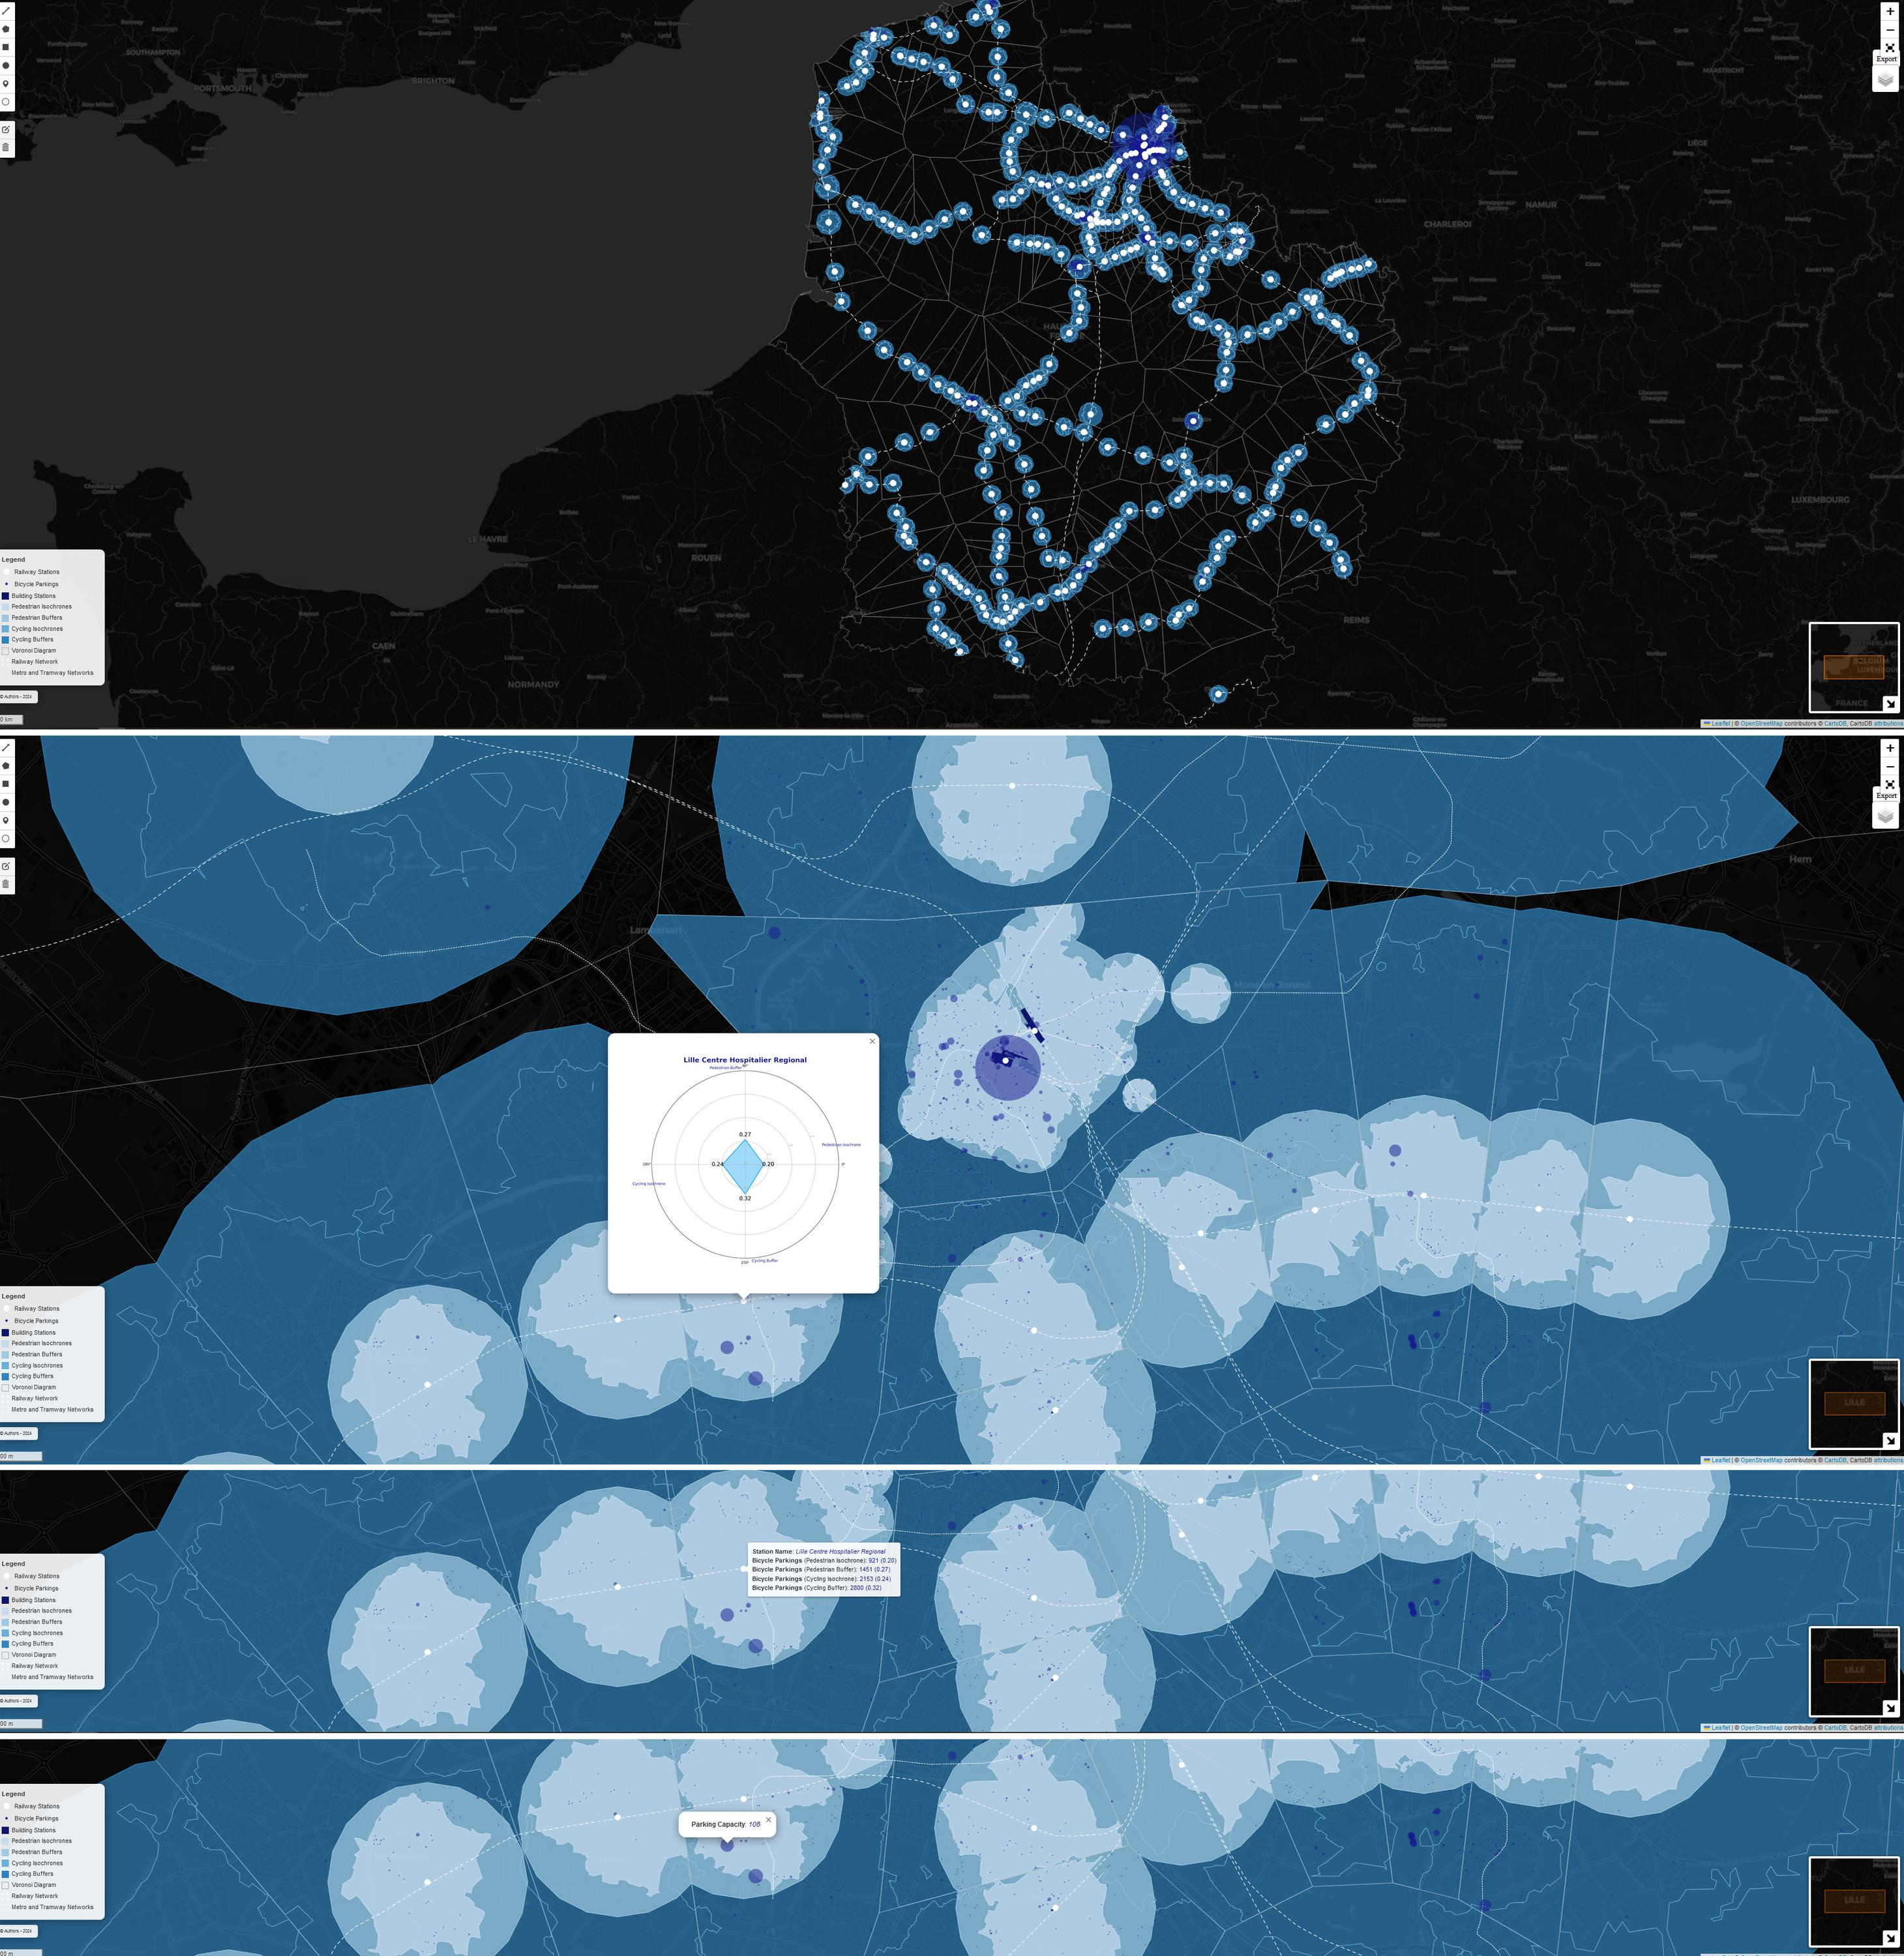
\includegraphics[width=1\columnwidth]{src/Figures/Chap-6/FR_EN_NPART_Carte_interactive.jpeg}}
        \vspace{5pt}
        \begin{flushright}\scriptsize{
        Réalisation~: \textcolor{blue}{Dylan Moinse (2024)}
        \\
        Auteur·rice·s~: projet de recherche \acrshort{NPART}
        }\end{flushright}
    \end{carte}

    % Carte fréquence des réseaux de TC
    %\begin{carte}[h!]\vspace*{4pt}
        %\caption{???.}
        %\label{fig-chap6:carte-frequence-reseaux-TC}
        %\centerline{\includegraphics[width=1\columnwidth]{src/Figures/Chap-6/FR_Carte_N1_N2_N3_N4.png}}
        %\vspace{5pt}
        %\begin{flushright}\scriptsize{
        % Réalisation~: \textcolor{blue}{Dylan Moinse (2024)}
        % \\
        % Auteur·rice·s~: projet de recherche \acrshort{NPART}
        %}\end{flushright}
    %\end{carte}

    % Limites
Si la valorisation de notre modèle constitue une étape clé pour garantir un projet scientifique abouti, nous sommes néanmoins conscients de certaines limitations. La principale contrainte en matière d’opérationnalisation réside, à nos yeux, dans l’absence d’une intégration complète des aménageur·se·s interrogé·e·s au sein du processus de modélisation. En effet, leur rôle s’est limité à la contribution de leurs opinions dans le cadre de la sélection et de la pondération statistique des critères \acrshort{TOD} et \acrshort{M-TOD}. Bien que nous ayons pris soin de leur transmettre les résultats de cette recherche, respectant ainsi l’engagement réciproque tenu avec les participant·e·s, il aurait été pertinent de les associer davantage en leur permettant de tester la carte dynamique, d’évaluer la modélisation proposée et, plus largement, de déterminer si celle-ci s’aligne sur les stratégies publiques définies.%%Rédigé%%

    % Transition vers chapitre~7
À cet égard, le travail de \textcolor{blue}{\textcite[784]{duffhues_breaking_2014}}\index{Duffhues, Jan|pagebf}\index{Mayer, Igor~S.|pagebf}\index{Nefs, Merten|pagebf}\index{Vliet, Mirte van der|pagebf} constitue une référence intéressante. Après avoir réalisé un \acrshort{NPM}, ces auteur·rice·s ont invité les parties prenantes à expérimenter leurs résultats sous la forme d’un jeu\footnote{
    La \Guillemets{gamification}, ou ludification de la recherche, consiste à intégrer des éléments ludiques et interactifs afin de stimuler l'engagement, l'appropriation et la motivation des participant·e·s et de valoriser les projets menés par les chercheur·se·s. En incorporant des mécanismes de jeu, les chercheur·se·s peuvent rendre leurs études notamment plus attractives et accessibles pour un public (non) spécialisé. La gamification favorise alors une appropriation accrue des contenus scientifiques par une audience élargie \textcolor{blue}{\autocite[6]{genvo_approche_2014}}\index{Genvo, Sébastien|pagebf}\index{Bonenfant, Maude|pagebf}, tandis que la ludification des processus de formation et de diffusion des connaissances peut renforcer la motivation des professionnel·le·s \textcolor{blue}{\autocite[36, 62]{lu_gamification_2023}}\index{Lu, Huihui|pagebf}. Dans le cadre du \acrshort{NPM} élaboré par \textcolor{blue}{\textcite[784]{duffhues_breaking_2014}}\index{Duffhues, Jan|pagebf}\index{Mayer, Igor~S.|pagebf}\index{Nefs, Merten|pagebf}\index{Vliet, Mirte van der|pagebf}, un jeu sérieux (\textsl{serious game}) intitulé \textsl{SPRINTCITY} a été mis en œuvre pour simuler l'aménagement d'un corridor ferroviaire sur une période de vingt ans. En dépit de la formulation de certaines critiques, il a été rapporté que ce jeu a permis de sensibiliser les acteur·rice·s aux bénéfices potentiels offerts par le \acrshort{TOD}, à l'importance stratégique de l'échelle géographique du corridor au-delà de la simple station, ainsi qu'aux conflits d'intérêt susceptibles d'émerger au cours du processus de planification urbaine.
}. Leurs observations ont mis en évidence que, pour ces praticien·ne·s, le modèle apparaissait trop axé sur une approche quantitative et pouvait être difficilement compréhensible, révélant ainsi des marges d’amélioration. Sur la base de cet enseignement, le prochain chapitre aborde cette limitation en cherchant à rendre le modèle plus tangible et accessible pour les aménageur·se·s. Nous nous appuyons pour cela sur la distinction établie par \textcolor{blue}{\textcite[499]{higgins_forty_2016}}\index{Higgins, Christopher~D.|pagebf}\index{Kanaroglou, Pavlos~S.|pagebf} qui démêlent l’approche \Guillemets{positive}~–~quantitative, systématique et empirique~–~de l’approche \Guillemets{normative}, visant à mieux décrire les types de \acrshort{TOD} à travers des étiquettes qualitatives. Dans cette optique, nous allons illustrer la classification déterminée à partir d’études de cas. Cette démarche consiste à donner un sens, dans une perspective aménagiste, plus sensible et contextuel aux classes formulées, en s’appuyant sur la réalisation de diagnostics territoriaux et la formulation de pistes d’aménagement à une échelle géographique plus fine et adaptée à chaque cas particulier.%%Rédigé%%

% ___________________________________________
     \newpage
     
% Valorisation scientifique
    \begin{tcolorbox}[colback=white!5!white,
                      colframe=blue!75!blue,
                      title=Valorisation scientifique
                      \\
                      Chapitre~6]
\Large{\textcolor{blue}{\textbf{Congrès internationaux~:}}}
    \\\\
\small{\textcolor{blue}{\textcite{moinse_enhancing_2024}}. Enhancing Transit-Oriented Development with Micro-mobility: A Renewed Node-Place Index Approach in the Hauts-de-France Region. \textsl{International Geographical Congress} (IGC), \textsl{\Guillemets{\foreignlanguage{english}{Transport and Geography: Sustainable transit-oriented development (STOD): new perspectives and advances}}}, Dublin.
\\
\footnotesize{\url{https://enpc.hal.science/hal-04682048}} (\textbf{C-ACTI})}
    \\\\
\Large{\textcolor{blue}{\textbf{Manifestations scientifiques~:}}}
    \\\\
\small{\textcolor{blue}{\textcite{moinse_revisiter_2024}}. Revisiter le modèle de « nœud-lieu » pour évaluer et classifier les quartiers de gare de la région Hauts-de-France. \textit{Séminaire mensuel du LVMT}, \Guillemets{Les variations de l'insertion urbaine des gares françaises et leur classification}, Paris.
\\
\footnotesize{\url{https://enpc.hal.science/hal-04620714}} (\textbf{C-COM})}
    \end{tcolorbox}

    % ___________________________________________
    % Sous-bibliographie
    \newpage
    \sectionheader{Sous-bibliographie du chapitre~6}
    \begingroup
    \renewcommand{\bibfont}{\scriptsize}
\printbibliography[segment=\therefsegment, heading=subbibintoc, title={Sous-bibliographie du chapitre~6}, label=chap6:bibliographie]
    \endgroup
    \end{refsegment}